\documentclass[10pt, letterpaper]{article}

% Inhaltsverzeichnis für Pakettypen (nur für Übersicht im Header, wird nicht im Dokument angezeigt)
% 1. Seitenlayout und Ränder
% 2. Sprache und Zeichensatz
% 3. Mathematik und Theorem-Umgebungen
% 4. Eigene Makros
% 5. Diagramme und Grafiken
% 6. Tabellen und Aufzählungen
% 7. Inhaltsverzeichnis
% 8. Abschnittsüberschriften
% 9. Abstrakt-Umgebung
% 10. Todos/Notizen
% 11. Rahmen/Box-Umgebungen
% 12. Python-Integration
% 13. Literaturverwaltung
% 14. Hyperlinks
% 15. Absatzeinstellungen
% 16. Umgebungen
% 17  Graphik
% 18  Extra
% 00. Titel und Autor

% --- 1. Seitenlayout und Ränder ---
\usepackage[margin=3cm]{geometry}

% --- 2. Sprache und Zeichensatz ---
\usepackage[english]{babel}
\usepackage[T1]{fontenc}
\usepackage[utf8]{inputenc}

% --- 3. Mathematik und Theorem-Umgebungen ---
\usepackage{amsmath, amssymb, amsthm}
\usepackage{mathrsfs}
\DeclareMathOperator{\WF}{WF}

% --- 4. Eigene Makros ---
\usepackage{xcolor}
\newcommand{\SKP}{\langle\cdot,\cdot\rangle}
\newcommand{\R}{\mathbb{R}}
\newcommand{\N}{\mathbb{N}}
\newcommand{\Q}{\mathbb{Q}}
\newcommand{\Z}{\mathbb{Z}}
\newcommand{\C}{\mathbb{C}}
\newcommand{\entwurf}[1]{\textcolor{red}{#1}}

% --- 5. Diagramme und Grafiken ---
\usepackage{graphicx}
\graphicspath{{../../Library/Images/}}
\usepackage[export]{adjustbox}
\usepackage{tikz}
\usetikzlibrary{decorations.pathreplacing, arrows.meta, positioning}
\usepackage{tikz-cd}

% --- 6. Tabellen und Aufzählungen ---
\usepackage{enumitem}
\setlist[itemize]{left=0.5cm}

\newenvironment{romanenum}[1][]
  {%
    \ifx&#1&
    \else
      \textbf{#1}\quad
    \fi
    \begin{enumerate}[label=\roman*)]
  }
  {%
    \end{enumerate}%
  }

% --- 7. Inhaltsverzeichnis ---
\usepackage{tocloft}
\renewcommand{\cftsecfont}{\footnotesize}
\renewcommand{\cftsubsecfont}{\footnotesize}
\renewcommand{\cftsubsubsecfont}{\footnotesize}
\renewcommand{\cftsecpagefont}{\footnotesize}
\renewcommand{\cftsubsecpagefont}{\footnotesize}
\renewcommand{\cftsubsubsecpagefont}{\footnotesize}
\usepackage{etoc}

% --- 8. Abschnittsüberschriften ---
\usepackage{titlesec}
\titleformat{\section}{\normalfont\large\bfseries}{\thesection}{1em}{}
\titleformat{\subsection}{\normalfont\normalsize\bfseries}{\thesubsection}{0.5em}{}
\titleformat{\subsubsection}{\normalfont\normalsize\bfseries}{\thesubsubsection}{0.5em}{}
\setcounter{secnumdepth}{4}

% --- 9. Abstrakt-Umgebung ---
\usepackage{changepage}
\renewenvironment{abstract}
  {
    \begin{adjustwidth}{1.5cm}{1.5cm}
    \small
    \textsc{Abstract. –}%
  }
  {
    \end{adjustwidth}
  }

% --- 10. Todos/Notizen ---
\usepackage{todonotes}

% --- 11. Rahmen/Box-Umgebungen ---
\usepackage{mdframed}
\usepackage{tcolorbox}
\colorlet{shadecolor}{gray!25}

\newenvironment{customTheorem}
  {\vspace{10pt}%
   \begin{mdframed}[
     backgroundcolor=gray!20,
     linewidth=0pt,
     innertopmargin=10pt,
     innerbottommargin=10pt,
     skipabove=\dimexpr\topsep+\ht\strutbox\relax,
     skipbelow=\topsep,
   ]}
  {\end{mdframed}
   \vspace{10pt}%
  }

% --- 12. Python-Integration ---
% (Deaktiviert in dieser Version, aktiviere bei Bedarf)
% \usepackage{pythontex}
% \usepackage[makestderr]{pythontex}

% --- 13. Literaturverwaltung ---
\usepackage{csquotes}
\usepackage[backend=biber, style=alphabetic, citestyle=alphabetic]{biblatex}
\addbibresource{bibliography.bib}

% --- 14. Hyperlinks ---
\usepackage{hyperref}
\hypersetup{
  colorlinks   = true,
  urlcolor     = blue,
  linkcolor    = blue,
  citecolor    = blue,
  frenchlinks  = true
}

% --- 15. Absatzeinstellungen ---
\usepackage[parfill]{parskip}
\sloppy

% --- 16. Umgebungen ---
\usepackage{thmtools}

\newcommand{\CustomHeading}[3]{%
  \par\medskip\noindent%
  \textbf{#1 #2} \textnormal{(#3)}.\enskip%
}

\newenvironment{DEF}[2]{\begin{unitbox}\CustomHeading{Definition}{#1}{#2}}{\end{unitbox}}
\newenvironment{PROP}[2]{\begin{unitbox}\CustomHeading{Proposition}{#1}{#2}}{\end{unitbox}}
\newenvironment{THEO}[2]{\begin{unitbox}\CustomHeading{Theorem}{#1}{#2}}{\end{unitbox}}
\newenvironment{LEM}[2]{\begin{unitbox}\CustomHeading{Lemma}{#1}{#2}}{\end{unitbox}}
\newenvironment{KORO}[2]{\begin{unitbox}\CustomHeading{Corollar}{#1}{#2}}{\end{unitbox}}
\newenvironment{REM}[2]{\begin{unitbox}\CustomHeading{Remark}{#1}{#2}}{\end{unitbox}}
\newenvironment{EXA}[2]{\begin{unitbox}\CustomHeading{Example}{#1}{#2}}{\end{unitbox}}
\newenvironment{STUD}[2]{\begin{unitbox}\CustomHeading{Study}{#1}{#2}}{\end{unitbox}}
\newenvironment{CONC}[2]{\begin{unitbox}\CustomHeading{Concept}{#1}{#2}}{\end{unitbox}}
\newenvironment{OTH}[2]{\begin{unitbox}\CustomHeading{Other}{#1}{#2}}{\end{unitbox}}
\newenvironment{EXE}[2]{\begin{unitbox}\CustomHeading{Exercise}{#1}{#2}}{\end{unitbox}}
\newenvironment{MOT}[2]{\begin{unitbox}\CustomHeading{Motivation}{#1}{#2}}{\end{unitbox}}
\newenvironment{PROOF}[2]{\begin{unitbox}\CustomHeading{Proof}{#1}{#2}}{\end{unitbox}}

% --- Unit Umgebung für Source-Inhalte ---
\usepackage{mdframed}
\newmdenv[
  linewidth=1pt,
  topline=false,
  bottomline=false,
  rightline=false,
  leftmargin=0cm,
  rightmargin=0cm,
  skipabove=10pt,
  skipbelow=10pt,
  innertopmargin=0.5\baselineskip,
  innerbottommargin=0.5\baselineskip,
  backgroundcolor=gray!10,
  linecolor=gray
]{unitbox}

\newenvironment{unit}[1]
  {\begin{unitbox}\textbf{Unit #1}\par\smallskip}
  {\end{unitbox}}

% --- 17. Graphik ---
% \usepackage{graphicx}
% \graphicspath{ {./images/} }


% --- 18. Extras ---
\usepackage{stmaryrd}
\usepackage{bbold}  % falls du \mathbb{1} nutzen willst

\usepackage{mathrsfs}

%New command to display footnote whose markers will always be hidden
\let\svthefootnote\thefootnote
\newcommand\blfootnotetext[1]{%
  \let\thefootnote\relax\footnote{#1}%
  \addtocounter{footnote}{-1}%
  \let\thefootnote\svthefootnote%
}

%Overriding the \footnotetext command to hide the marker if its value is `0`
\let\svfootnotetext\footnotetext
\renewcommand\footnotetext[2][?]{%
  \if\relax#1\relax%
    \ifnum\value{footnote}=0\blfootnotetext{#2}\else\svfootnotetext{#2}\fi%
  \else%
    \if?#1\ifnum\value{footnote}=0\blfootnotetext{#2}\else\svfootnotetext{#2}\fi%
    \else\svfootnotetext[#1]{#2}\fi%
  \fi
}

% --- 00. Titel und Autor ---
\title{Mein Titel}
\author{Tim Jaschik}
\date{\today}




\begin{document}

\maketitle
\rule{\textwidth}{0.5pt}
\begin{abstract}
Kurze Beschreibung …
\end{abstract}
\rule{\textwidth}{0.5pt}
\vspace{0.5cm}




\tableofcontents

\pagebreak


\section*{Teil 1. Gruppen}
\section*{Gruppen und Homomorphismen}
1.1. Definition und erste Beispiele. Wir beginnnen mit der grundlegenden Definition.

Definition 1.1. Eine Gruppe ist ein Paar ( $G, \circ$ ) bestehend aus einer Menge $G$ und einer Verknüpfung

$$
\circ: G \times G \rightarrow G,
$$

geschrieben als $(g, h) \mapsto g \circ h$, mit den folgenden Eigenschaften.\\
(i) Die Verknüpfung ist assoziativ: für alle $g, h, k \in G$ gilt:

$$
g \circ(h \circ k)=(g \circ h) \circ k
$$

Die Klammerung legt die Reihenfolge fest, in der die Verknüpfungen auszuführen sind.\\
(ii) Es gibt ein Element $e \in G$, neutrales Element genannt, so daß für alle $g \in G$

$$
g \circ e=g=e \circ g
$$

(iii) Zu jedem $g \in G$ gibt es ein $h \in G$, inverses Element oder das Inverse genannt, so daß

$$
g \circ h=e=h \circ g .
$$

Notation 1.2. Wir vereinfachen sofort die Notation und unsere Vorstellung, was eine Gruppe ist.\\
(1) Bei einer Gruppe ( $G, \circ$ ) denkt man zuerst an die zugrundeliegende Menge $G$ und sodann an die auf $G$ definierte Verknüpfung. Um die Notation zu verkürzen und damit knapp und übersichtlicher zu halten, sagen wir "Sei G eine Gruppe ...", wenn wir in Wahrheit die Menge zusammen mit der Verknüpfung meinen. In der Regel ist die gemeinte Verknüpfung die offensichtliche Verknüpfung und es entstehen keine Mißverständnisse.\\
(2) Um die Verknüpfung zweier Gruppenelemente $g$ und $h$ zu bezeichnen, sind verschiedenste Notationen gebräuchlich, etwa

$$
g h, g+h, g * h, g \circ h, \ldots
$$

Bemerkung 1.3. (1) Die Assoziativität sorgt dafür, daß für $g_{1}, \ldots, g_{r} \in G$ das Element

$$
g_{1} g_{2} \ldots g_{r} \in G
$$

als Ergebnis von $r-1$ Verknüpfungen benachbarter Elemente unabhängig von der vorhandenen Wahl ist. Das ist unmittelbar klar, muß aber, wie alle Dinge die offensichtlich sind, bewiesen werden. Das gelingt durch vollständige Induktion nach der Länge $r$, aber damit wollen wir uns nicht aufhalten und überlassen das als Übungsaufgabe.\\
(2) Man kann die Axiome einer Gruppe abschwächen und zu einem äquivalenten Begriff kommen, wenn man nur die Existenz eines linksneutralen Elements und eines Linksinversen verlangt. Die Liste der Eigenschaften in Definition 1.1 ist aber diejenige, die man mit einer Gruppe verbinden sollte, und daher sprechen wir die Definition derart aus.

Beispiel 1.4. Beispiele für Gruppen sind bereits bekannt. Die wichtigsten in der linearen Algebra aufgetretenen Gruppen sind die folgenden.\\
(1) Die ganzen Zahlen $\mathbb{Z}$ mit Addition bilden eine Gruppe.\\
(2) Sei $n \geq 1$ eine natürliche Zahl. Die symmetrische Gruppe

$$
S_{n}
$$

ist die Menge aller Permutationen (bijektiven Selbstabbildungen) der Menge $\{1, \ldots, n\}$ mit der Komposition von Permutationen als Verknüpfung. Die symmetrische Gruppe ist nichts weiter als die volle Gruppe der Symmetrien der unstrukturierten Menge von $n$ Elementen.\\
(3) Sei $K$ ein Körper und $V$ ein $K$-Vektorraum. Dann ist die Menge

$$
\mathrm{GL}(V)
$$

der bijektiven linearen Abbildungen $f: V \rightarrow V$ die allgemeine ${ }^{3}$ lineare Gruppe von $V$. Die Gruppenverknüpfung hier ist wieder die Komposition und GL( $V$ ) ist die volle Gruppe der Symmetrien der Menge $V$, welche die $K$-lineare Vektorraumstruktur erhalten.

Speziell für $V=K^{n}$ setzen wir

$$
\operatorname{GL}_{n}(K)=\operatorname{GL}\left(K^{n}\right)=\left\{A \in \mathrm{M}_{n}(K) ; \operatorname{det}(A) \neq 0\right\}
$$

beschrieben durch invertierbare $n \times n$-Matrizen mit Einträgen aus $K$.\\
(4) Sei $K$ ein Körper. Die multiplikative Gruppe von $K$ ist die Teilmenge

$$
K^{\times}=K \backslash\{0\}
$$

mit der Multiplikation als Verknüpfung. Es ist geradezu die Definition eines Körpers: ein Ring $K$, für den $(K \backslash\{0\}, \cdot)$ eine Gruppe bildet.\\
(5) Die kleinste Gruppe ist $G=\{e\}$ mit der einzig möglichen Verknüpfung $e e=e$. Diese Gruppe nennt man die triviale Gruppe.

Bemerkung 1.5. Man sollte der Versuchung widerstehen, eine (endliche) Gruppe durch ihre Verknüpfungstafel, also eine Tabelle, welche die Werte $g h$ mit $g, h \in G$ angibt, verstehen zu wollen. Zum Beispiel für eine Gruppe mit zwei Elementen $G=\{e, g\}$ :

\begin{center}
\begin{tabular}{c|cc}
 & $e$ & $g$ \\
\hline
$e$ & $e$ & $g$ \\
$g$ & $g$ & $e$ \\
\end{tabular}
\end{center}

Die dargestellte Information ist vollständig, aber auch vollständig nutzlos zum Verständnis. Wenigstens kann man sich mit diesem Beispiel leicht davon überzeugen, daß es im Wesentlichen (bis auf Bezeichnungen) nur eine Gruppe mit zwei Elementen gibt. Eine nützliche Beschreibung dieser Gruppe bekommt man als Gruppe

$$
\{1,-1\}
$$

etwa als Teilmenge von $\mathbb{R}$ mit der Multiplikation als Verknüpfung. Dabei ist $e=1$ und $g=-1$.\\
Definition 1.6. Zwei Elemente $g, h$ einer Gruppe $G$ kommutieren (miteinander), wenn

$$
g h=h g
$$

Kommutieren in einer Gruppe alle Elemente miteinander, dann spricht man von einer kommutativen oder abelschen ${ }^{4}$ Gruppe.

Beispiel 1.7. Auch Beispiele abelscher Gruppen sind bereits bekannt.\\
(1) Die ganzen Zahlen $(\mathbb{Z},+)$ sind eine abelsche Gruppe.\\
(2) Sei $n \in \mathbb{Z}$. Wir erinnern daran, daß wir für $a, b \in \mathbb{Z}$ sagen „a ist kongruent zu $b$ modulo $n$ " mit Notation $a \equiv b(\bmod n)$, wenn es ein $k \in \mathbb{Z}$ gibt mit $a-b=k n$. Die Relation kongruent modulo $n$ ist eine Äquivalenzrelation auf $\mathbb{Z}$. Die Restklassen modulo $n$ bilden mit der auf Vertretern der Restklassen definierten Addition eine abelsche Gruppe

$$
\mathbb{Z} / n \mathbb{Z}
$$

Darin bezeichnen wir mit $[a]$ die Restklasse $a+n \mathbb{Z}$ zum Vertreter $a \in \mathbb{Z}$.\\
Das spezielle Beispiel $n=12$ zusammen mit der modularen Arithmetik modulo 12 lernt jedes Kind zusammen mit der Uhr in der Regel spätestens in der Grundschule.\\
(3) Sei $K$ ein Körper und sei $V$ ein $K$-Vektorraum. Dann ist $V$ mit der Addition aus der Vektorraumstruktur eine abelsche Gruppe ( $V,+$ ).

\footnotetext{${ }^{3}$ Englisch: general linear group, daher GL.\\
${ }^{4}$ Niels Henrik Abel, 1802-1829, norwegischer Mathematiker.
}Bemerkung 1.8. (1) Die Kommutativität sorgt dafür, daß in einer kommutativen Gruppe $G$ für $g_{1}, \ldots, g_{n} \in G$ das Element

$$
g_{1} g_{2} \ldots g_{n} \in G
$$

unabhängig von der Reihenfolge ist: Für jede Permutation $\sigma \in S_{n}$ gilt

$$
g_{1} g_{2} \ldots g_{r}=g_{\sigma(1)} g_{\sigma(2)} \ldots g_{\sigma(n)}
$$

(2) Es gibt einen Struktursatz für endlich erzeugte abelsche Gruppen. Dieser benutzt weniger Methoden der Gruppentheorie, sondern solche der kommutativen Algebra, wie sie im Kapitel über Ringe und Moduln behandelt werden, und wird daher erst später behandelt.

Definition 1.9. (1) Das direkte Produkt zweier Gruppen $G_{1}$ und $G_{2}$ ist die Gruppe

$$
G_{1} \times G_{2}=\left\{\left(g_{1}, g_{2}\right) ; g_{1} \in G_{1}, g_{2} \in G_{2}\right\}
$$

mit komponentenweiser Komposition als Verknüpfung.\\
(2) Das direkte Produkt einer Menge $G_{i}$ von Gruppen für $i \in I$ ist die Gruppe

$$
\prod_{i \in I} G_{i}=\left\{\left(g_{i}\right)_{i \in I} ; g_{i} \in G_{i} \text { für alle } i \in I\right\}
$$

mit komponentenweiser Komposition als Verknüpfung.\\
Bemerkung 1.10. Das direkte Produkt zweier Gruppen ist ein Spezialfall der allgemeinen Konstruktion für $I=\{1,2\}$. Das neutrale Element in $\prod_{i \in I} G_{i}$ ist

$$
\left(e_{i}\right)_{i \in I}
$$

wobei $e_{i} \in G_{i}$ das neutrale Element ist. Die Komposition zweier Elemente ist

$$
\left(g_{i}\right)_{i \in I}\left(h_{i}\right)_{i \in I}=\left(g_{i} h_{i}\right)_{i \in I}
$$

Das Inverse von $\left(g_{i}\right)_{i \in I}$ ist

$$
\left(g_{i}\right)_{i \in I}^{-1}=\left(g_{i}^{-1}\right)_{i \in I}
$$

1.2. Elementare Folgerungen. Die Definition einer Gruppe hat einige unmittelbare Konsequenzen für neutrale und inverse Elemente.

Proposition 1.11. In jeder Gruppe ist das neutrale Element eindeutig.\\
Beweis. Seien $e$ und $e^{\prime}$ neutrale Elemente einer Gruppe $G$. Dann gilt

$$
e=e e^{\prime}=e^{\prime}
$$

Notation 1.12. Das nach Proposition 1.11 eindeutige neutrale Element $e \in G$ wird oft mit 1 oder 0 bezeichnet je nachdem, ob man bei der Verknüpfung an eine Multiplikation oder eine Addition denkt. Beispielsweise ist $1 \in \mathrm{GL}_{n}(K)$ eine Kurznotation für die Einheitsmatrix. Dies ist nur eine Sprechweise und bedeutet sonst nichts.

Proposition 1.13. In jeder Gruppe ist das Inverse eines Elements eindeutig.\\
Genauer: sei $g \in G$ ein Element einer Gruppe $G$ und $h \in G$ mit

$$
h g=e
$$

dann ist h das Inverse von $g$. Hier bezeichnet e das neutrale Element von $G$.\\
Beweis. Sei $k$ ein Inverses zu $g$. Dies existiert nach den Gruppenaxiomen. Dann gilt

$$
h=h e=h(g k)=(h g) k=e k=k
$$

Also ist $h=k$ ein Inverses.\\
Dasselbe Argument zeigt auch die Eindeutigkeit: sind $h$ und $k$ Inverse zu $g$, dann gilt $h g=e$, man kann $k$ wie im obigen Argument wählen und schließt auf $h=k$.

Notation 1.14. Das nach Proposition 1.13 eindeutige Inverse zu einem Element $g \in G$ wird mit

$$
g^{-1}
$$

bezeichnet, sofern die Verknüpfung multiplikativ geschrieben wird. Wird die Verknüpfung additiv geschrieben, wie das bei abelschen Gruppen üblich ist, so verwenden wir für das Inverse zu $g$ die Notation $-g$.\\
Proposition 1.15. Für Elemente $g$, $h$ einer Gruppe gilt\\
(1) $(g h)^{-1}=h^{-1} g^{-1}$,\\
(2) $\left(g^{-1}\right)^{-1}=g$.

Beweis. (1) Wir berechnen

$$
\left(h^{-1} g^{-1}\right)(g h)=h^{-1}\left(g^{-1} g\right) h=h^{-1} h=e .
$$

und schließen nach Proposition 1.13, daß $h^{-1} g^{-1}$ das Inverse zu $g h$ ist.\\
(2) Es gilt $g\left(g^{-1}\right)=e$, somit ist $g$ Inverses zu $g^{-1}$. Die Eindeutigkeit des Inversen nach Proposition 1.13 zeigt $g=\left(g^{-1}\right)^{-1}$.\\
1.3. Gruppenhomomorphismen. Um Gruppen besser zu verstehen, braucht man einen Begriffsapparat für den Vergleich von Gruppen: strukturerhaltende Abbildungen.

Definition 1.16. Ein Gruppenhomomorphismus (oder Homomorphismus von Gruppen) ist eine Abbildung

$$
f: G \rightarrow H
$$

von einer Gruppe $G$ nach einer Gruppe $H$ mit der Eigenschaft, daß für alle $a, b \in G$ gilt:

$$
f(a b)=f(a) f(b)
$$

Beispiel 1.17. Auch für Gruppenhomomorphismen kennen wir bereits einige Beispiele.\\
(1) Die Determinante ist ein Gruppenhomomorphismus

$$
\operatorname{det}: \mathrm{GL}_{n}(K) \rightarrow K^{\times} .
$$

(2) Das aus der linearen Algebra bekannte Signum einer Permutation ist ein Gruppenhomomorphismus

$$
\operatorname{sign}: S_{n} \rightarrow\{ \pm 1\}
$$

Das Signum einer Transposition $\tau \in S_{n}$ ist $\operatorname{sign}(\tau)=-1$. Weil jede Permutation $\sigma \in S_{n}$ als Komposition von Transpositionen $\tau_{i}$ geschrieben werden kann, etwa

$$
\sigma=\tau_{1} \cdots \tau_{s}
$$

legt die Homomorphie das Signum dadurch eindeutig fest:

$$
\operatorname{sign}(\sigma)=\operatorname{sign}\left(\tau_{1}\right) \cdots \operatorname{sign}\left(\tau_{s}\right)=(-1)^{s}
$$

Es gibt somit höchstens einen Homomorphismus sign : $S_{n} \rightarrow\{ \pm 1\}$ mit dem Wert -1 auf den Transpositionen.

Die Existenz des Signum ist eine nichttriviale Sache: Die Anzahl an Transpositionen, die man für eine Permutation braucht, ist modulo 2 unabhängig von der Wahl der Transpositionen.

Am einfachsten ${ }^{5}$ sieht man die Existenz des Signum über die Determinante der Permutationsmatrizen ein. Sei $\sigma \in S_{n}$. Dann ist $P_{\sigma} \in \mathrm{GL}_{n}(\mathbb{Q})$ die Matrix, deren $j$-te Spalte $e_{\sigma(j)}$ ist. Es gilt also

$$
P_{\sigma}\left(e_{j}\right)=e_{\sigma(j)}
$$

\footnotetext{${ }^{5}$ Hier droht ein Zirkelschluß, denn oft wird die Existenz der Determinante durch eine Formel bewiesen, die das Signum der Permutationen benötigt.
}
die Permutationsmatrix permutiert die Standardbasis wie dies $\sigma$ vorschreibt. Daher gilt für $\sigma, \pi \in S_{n}$ :
$$
P_{\sigma \pi}=P_{\sigma} P_{\pi}
$$
denn für alle $j=1, \ldots, n$ gilt
$$
P_{\sigma \pi}\left(e_{j}\right)=e_{\sigma \pi(j)}=e_{\sigma(\pi(j))}=P_{\sigma}\left(e_{\pi(j)}\right)=P_{\sigma}\left(P_{\pi}\left(e_{j}\right)\right)=\left(P_{\sigma} \circ P_{\pi}\right)\left(e_{j}\right)
$$

Die Zuordnung $\rho(\sigma)=P_{\sigma}$ ist ein Gruppenhomomorphismus

$$
\rho: S_{n} \rightarrow \mathrm{GL}_{n}(\mathbb{Q}),
$$

den wir die Permutationsdarstellung von $S_{n}$ nennen.\\
Das Signum bekommen wir nun als Komposition

$$
\operatorname{sign}(\sigma)=\operatorname{det}(\rho(\sigma))
$$

In der Tat ist dies ein Gruppenhomomorphismus und nimmt auf Transpositionen nach Eigenschaft der Determinante den Wert -1 an.\\
(3) Sei $n \in \mathbb{Z}$. Die Addition auf $\mathbb{Z} / n \mathbb{Z}$ ist gerade so gemacht, daß die Restklassenabbildung

$$
\mathbb{Z} \rightarrow \mathbb{Z} / n \mathbb{Z}, \quad a \mapsto a+n \mathbb{Z}
$$

ein Gruppenhomomorphismus ist.\\
(4) Sei $f: V \rightarrow W$ eine lineare Abbildung von $K$-Vektorräumen. Dann ist $f$ ein Gruppenhomomorphismus der zugrundeliegenden abelschen Gruppen ( $V,+$ ) und ( $W,+$ ).\\
(5) Sei $I$ eine Menge und sei $G_{i}$ eine Gruppe für $i \in I$. Sei $n \in I$ ein Element. Die Projektion auf die $n$-te Koordinate des Produkts

$$
p_{n}: \prod_{i \in I} G_{i} \rightarrow G_{n}
$$

ist der Gruppenhomomorphismus mit $p_{n}\left(\left(g_{i}\right)_{i \in I}\right)=g_{n}$. Die Homomorphieeigenschaft folgt sofort aus der Definition des Produkts, weil die Gruppenverknüpfung im Produkt komponentenweise erklärt ist.

Lemma 1.18. Sei $G$ eine Gruppe. Das neutrale Element von $G$ ist das einzige Element $g \in G$ mit $g g=g$.

Beweis. Sei $e \in G$ das neutrale Element. Dann gilt $e e=e$. Für die umgekehrte Richtung betrachten wir ein $g \in G$ mit $g g=g$. Dann ist

$$
e=g^{-1} g=g^{-1}(g g)=\left(g^{-1} g\right) g=e g=g .
$$

Lemma 1.19. Sei $f: G \rightarrow H$ ein Gruppenhomomorphismus.\\
(1) Es gilt

$$
f\left(e_{G}\right)=e_{H}
$$

wobei $e_{G}$ das neutrale Element in $G$ und $e_{H}$ das in $H$ bezeichne.\\
(2) Für alle $g \in G$ gilt

$$
f\left(g^{-1}\right)=f(g)^{-1}
$$

Beweis. (1) Aus $f\left(e_{G}\right)=f\left(e_{G} e_{G}\right)=f\left(e_{G}\right) f\left(e_{G}\right)$ folgt $f\left(e_{G}\right)=e_{H}$ nach Lemma 1.18.\\
(2) Sei nun wieder $e \in G$ das neutrale Element. Wegen (1) gilt für $g \in G$

$$
f(g) f\left(g^{-1}\right)=f\left(g g^{-1}\right)=f(e)=e
$$

Daraus folgt mit Proposition 1.13 die Behauptung.\\
Definition 1.20. Ein Isomorphismus (von Gruppen) ist ein bijektiver Gruppenhomomorphismus, und ein Automorphismus (von Gruppen) ist ein Isomorphismus $G \rightarrow G$.

Zwei Gruppen $G$ und $H$ heißen isomorph, wenn es einen Isomorphismus $G \rightarrow H$ zwischen ihnen gibt. Als Notation verwenden wir $G \simeq H$.

Beispiel 1.21. Die positiven reellen Zahlen $\mathbb{R}_{>0} \subseteq \mathbb{R}^{\times}$bilden mit Multiplikation eine Gruppe. Die Exponentialfunktion nimmt nur Werte in $\mathbb{R}_{>0}$ an und liefert einen Gruppenhomomorphismus

$$
\exp : \mathbb{R} \rightarrow \mathbb{R}_{>0}
$$

denn für alle $x, y \in \mathbb{R}$ gilt

$$
\exp (x+y)=\exp (x) \exp (y)
$$

Dies ist sogar ein Isomorphismus. Die Umkehrabbildung ist der natürliche Logarithmus.\\
Proposition 1.22. Es gilt:\\
(1) Die Komposition von Gruppenhomomorphismen ist wieder ein Gruppenhomomorphismus.\\
(2) Die Identität ist ein Gruppenhomomorphismus.\\
(3) Ein bijektiver Gruppenhomomorphismus hat eine links- und rechtsinverse Abbildung bezüglich der Komposition, welche selbst Gruppenhomomorphismus ist.

Beweis. (1) Seien $g: G \rightarrow H$ und $f: H \rightarrow K$ Gruppenhomomorphismen. Dann gilt für alle $a, b \in G$ für $h=f \circ g$, daß

$$
h(a b)=f(g(a b))=f(g(a) g(b))=f(g(a)) f(g(b))=h(a) h(b),
$$

und damit ist $h$ auch ein Gruppenhomomorphismus.\\
Aussage (2) ist trivial.\\
(3) Sei $f: G \rightarrow H$ bijektiver Gruppenhomomorphismus. Dann gibt es $f^{-1}: H \rightarrow G$ als Mengenabbildung mit der Eigenschaft $f \circ f^{-1}=\operatorname{id}_{H}$ und $f^{-1} \circ f=\operatorname{id}_{G}$. Es bleibt zu zeigen, daß $f^{-1}$ ein Gruppenhomomorphismus ist. Dazu benutzen wir die Bijektivität von $f$ und beschreiben zwei beliebige Elemente $x, y \in H$ durch $a, b \in G$ als $x=f(a), y=f(b)$. Wir rechnen nun

$$
f^{-1}(x y)=f^{-1}(f(a) f(b))=f^{-1}(f(a b))=a b=f^{-1}(x) f^{-1}(y)
$$

und dies weist $f^{-1}$ als Gruppenhomomorphismus aus.\\
Korollar 1.23. Die Menge $\operatorname{Aut}(G)$ aller Automorphismen einer Gruppe $G$ ist bezüglich der Komposition eine Gruppe.

Beispiel 1.24. Sei $p$ eine Primzahl und $\mathbb{F}_{p}=\mathbb{Z} / p \mathbb{Z}$ der Körper mit $p$ Elementen. Sei $n$ eine natürliche Zahl. Die Skalarmultiplikation auf dem $\mathbb{F}_{p}$-Vektorraum $\mathbb{F}_{p}^{n}$ wird schon durch die Addition der zugrundeliegenden abelschen Gruppe erklärt. Genauer, sei $v \in \mathbb{F}_{p}^{n}$ ein Vektor, und sei der Skalar $\alpha \in \mathbb{F}_{p}$ repräsentiert durch $a \in \mathbb{N}$, dann ist $\alpha v$ durch

$$
\alpha v=\underbrace{v+\ldots+v}_{a \text {-mal }}
$$

erklärt. Dies hat zur Folge, daß $\mathbb{F}_{p}$-lineare Abbildungen von $\mathbb{F}_{p}$-Vektorräumen dasselbe sind wie Gruppenhomomorphismen der zugrundeliegenden abelschen Gruppen. Die Verträglichkeit mit der Skalarmultiplikation ist automatisch. Daraus folgt

$$
\operatorname{Aut}\left(\mathbb{F}_{p}^{n}\right)=\operatorname{GL}_{n}\left(\mathbb{F}_{p}\right)
$$

\section*{Übungsaufgaben ZU §1}
Übungsaufgabe 1.1. Zeigen Sie, daß in einer Gruppe $G$ für Elemente $g_{1}, \ldots, g_{r} \in G$ die Verknüpfung

$$
g_{1} \ldots g_{r}
$$

von der konkret gewählten Klammerung unabhängig ist.\\
Übungsaufgabe 1.2. Seien $g_{1}, \ldots, g_{n}$ Elemente einer kommutativen Gruppe $G$. Zeigen Sie, daß für jede Permutation $\sigma \in S_{n}$ gilt:

$$
g_{1} g_{2} \ldots g_{r}=g_{\sigma(1)} g_{\sigma(2)} \ldots g_{\sigma(n)}
$$

Übungsaufgabe 1.3. Sei $G=\{e, g\}$ eine Gruppe mit genau zwei Elementen: mit neutralem Element $e$ und $g \neq e$.\\
(a) Zeigen Sie, daß dann $g g=e$ gelten muß.\\
(b) Finden Sie einen Isomorphismus $G \simeq \mathbb{Z} / 2 \mathbb{Z}$.

Bemerkung: Sie zeigen hier, daß es bis auf Isomorphismus genau eine Gruppe mit zwei Elementen gibt. Darüberhinaus ist selbst der Isomorphismus zwischen zwei Gruppen der Ordnung 2 eindeutig.\\
Übungsaufgabe 1.4. In der Regel gilt für Elemente $g, h \in G$ und $n \in \mathbb{Z}$ nicht

$$
(g h)^{n}=g^{n} h^{n}
$$

Finden Sie ein Beispiel. Zeigen Sie, wenn dies für $n=-1$ und $g, h$ gilt, dann kommutieren $g, h$, und dann gilt die Gleichung bereits für alle $n \in \mathbb{Z}$.

Übungsaufgabe 1.5. Sei $G$ eine Gruppe und $\mu: G \times G \rightarrow G$ die Komposition. Zeigen Sie, daß $\mu$ denau dann ein Gruppenhomomorphismus ist, wenn $G$ abelsch ist.

Übungsaufgabe 1.6. Sei $G$ eine endliche Gruppe. Zeigen Sie, daß dann auch Aut $(G)$ eine endliche Gruppe ist.

\section*{Untergruppen}
In diesem Kapitel betrachten wir Teilmengen einer Gruppe, die selbst mit der gegebenen Gruppenverknüpfung Gruppen sind.\\
2.1. Das Untergruppenkriterium. Ein erstes Verständnis einer Gruppe erlangt man durch das Studium ihrer inneren Struktur, etwa ihrer Untergruppen.

Definition 2.1. Eine Untergruppe einer Gruppe $G$ ist eine Teilmenge $U \subseteq G$, so daß für alle $g, h \in U$ auch $g h \in U$ und $U$ mit der Einschränkung

$$
\begin{aligned}
U \times U & \rightarrow U \\
(g, h) & \mapsto g h
\end{aligned}
$$

der Verknüpfung von $G$ selbst eine Gruppe ist.\\
Bemerkung 2.2. Der zweite Teil der Definition ist nur aufgrund des ersten Teils wohldefiniert: die Einschränkung der Verknüpfung auf $U \times U \subseteq G \times G$ ist nur dann eine Verknüpfung auf $U$, also mit Werten in $U$, wenn man dies zuerst gefordert hat.

Notation 2.3. Wir werden eine Untergruppe $U$ einer Gruppe $G$ oft durch $U<G$ oder $U \leq G$ bezeichnen. Diese Notation ist aber nicht allgemeingültiger Standard.

Beispiel 2.4. (1) Die positiven reellen Zahlen mit Multiplikation bilden eine Untergruppe

$$
\mathbb{R}_{>0} \subseteq \mathbb{R}^{\times}
$$

(2) Sei $n \in \mathbb{Z}$. Die Menge $n \mathbb{Z}$ der durch $n$ teilbaren ganzen Zahlen ist eine Untergruppe

$$
n \mathbb{Z}=\{a \in \mathbb{Z} ; a=n x \text { für ein } x \in \mathbb{Z}\} \subseteq \mathbb{Z} .
$$

(3) In jeder Gruppe $G$ sind die triviale Gruppe $\{e\}$ und die ganze Gruppe $G$ Untergruppen.\\
(4) Die Teilmenge

$$
\{ \pm 1\} \subset \mathbb{Q}^{\times}
$$

ist eine Untergruppe (das ist gerade $\mathbb{Z}^{\times}$, vgl Kapitel §6).\\
(5) Die rationalen Matrizen $\mathrm{GL}_{n}(\mathbb{Q}) \subseteq \mathrm{GL}_{n}(\mathbb{R})$ sind eine Untergruppe. Allgemeiner haben wir für eine beliebige Körpererweiterung $K \subseteq L$ die Untergruppe

$$
\mathrm{GL}_{n}(K) \subseteq \mathrm{GL}_{n}(L) .
$$

(6) Die orthogonale Gruppe

$$
\mathrm{O}_{n}(K)=\left\{A \in \mathrm{M}_{n}(K) ; A^{t} A=\mathbf{1}_{n}\right\}
$$

ist eine Untergruppe von $\mathrm{GL}_{n}(K)$.\\
(7) Die Menge Aff ${ }^{1}(K)=K^{\times} \times K$ kann man als invertierbare affin-lineare Transformationen des 1-dimensionalen Vektorraums $K$ begreifen. Ein $(a, b) \in \operatorname{Aff}^{1}(K)$ beschreibt

$$
x \mapsto a x+b .
$$

Die Komposition von Abbildungen definiert eine Verknüpfung auf $\operatorname{Aff}^{1}(K)$ :

$$
(a x+b) \circ(c x+d)=(a(c x+d)+b)=a c x+a d+b
$$

also

$$
(a, b)(c, d):=(a c, a d+b)
$$

Dies ist die affin-lineare Gruppe in Dimension 1 (Übung!). Die Teilmengen

$$
U=\left\{(a, 0) ; a \in K^{\times}\right\}
$$

ist eine Untergruppe isomorph zu $K^{\times}$und

$$
V=\{(0, b) ; b \in K\}
$$

ist eine Untergruppe isomorph zu ( $K,+$ ).\\
(8) Die Menge Aff ${ }^{n}(K)=\mathrm{GL}_{n}(K) \times K^{n}$ kann man als invertierbare affin-lineare Transformationen Vektorraums $K^{n}$ begreifen. Ein $(A, b) \in \operatorname{Aff}^{n}(K)$ beschreibt

$$
x \mapsto A x+b .
$$

Die Komposition von Abbildungen definiert eine Verknüpfung auf $\operatorname{Aff}^{n}(K)$ :

$$
(A x+b) \circ(C x+d)=(A(C x+d)+b)=A C x+A d+b
$$

also

$$
(A, b)(C, d):=(A C, A d+b)
$$

Dies ist die affin-lineare Gruppe in Dimension $n$ (Übung!). Die Teilmengen

$$
U=\left\{(A, 0) ; A \in \mathrm{GL}_{n}(K)\right\}
$$

ist eine Untergruppe isomorph zu $\operatorname{GL}_{n}(K)$ und

$$
V=\left\{(0, b) ; b \in K^{n}\right\}
$$

ist eine Untergruppe isomorph zu ( $K^{n},+$ ).\\
(9) Sei $K$ ein Körper, sei $V$ ein $K$-Vektorraum und sei $U \subseteq V$ ein Untervektorraum. Dann ist $(U,+)$ eine Untergruppe von $(V,+)$.

Lemma 2.5. Sei $U \leq G$ eine Untergruppe.\\
(1) Das neutrale Element von $G$ ist auch das neutrale Element von $U$.\\
(2) Sei $u \in U$ und $u^{-1}$ das zu $u$ in $G$ inverse Element. Dann ist $u^{-1} \in U$ und in $U$ das zu $u$ inverse Element.

Beweis. (1) Sei $\varepsilon \in U$ neutrales Element für die Gruppe $U$. Aus $\varepsilon \varepsilon=\varepsilon$ in $U$ folgt mit Lemma 1.18, daß $\varepsilon$ auch neutrales Element von $G$ ist.\\
(2) Sei $u \in U$ beliebig, $u^{-1}$ das inverse Element in $G$ und $v \in U$ das inverse Element in $U$. Dann gilt (mit (1))

$$
u^{-1}=u^{-1} e=u^{-1}(u v)=\left(u^{-1} u\right) v=e v=v \in U
$$

Notation 2.6. Für Teilmengen $A, B \subseteq G$ einer Gruppe $G$ und ein Element $g \in G$ vereinbaren wir die Notationen

$$
\begin{aligned}
A B & :=\{a b ; a \in A, b \in B\}, \\
g A & :=\{g a ; a \in A\}, \\
A g & :=\{a g ; a \in A\}, \\
A^{-1} & :=\left\{a^{-1} ; a \in A\right\} .
\end{aligned}
$$

Analog zum Unterraumkriterium für Untervektorräume gibt es wie folgt ein Kriterium zum Nachweis, ob eine Teilmenge eine Untergruppe ist.

Proposition 2.7 (Untergruppenkriterium). Sei $U$ eine Teilmenge einer Gruppe G. Es bezeichne $e \in G$ das neutrale Element. Dann sind äquivalent:\\
(a) $U$ ist Untergruppe.\\
(b) Es gilt $e \in U$, sowie $U U \subseteq U$ und $U^{-1} \subseteq U$.\\
(c) $U$ ist nicht leer und für alle $u, v \in U$ folgt $u v^{-1} \in U$.

Beweis. Wir zeigen im Ringschluß (a) $\Longrightarrow$ (b) $\Longrightarrow$ (c) $\Longrightarrow$ (a).\\
$(a) \Longrightarrow(b)$ : Es gelte Aussage (a). Dann enthält $U$ das neutrales Element nach Lemma 2.5. Und per Defintion gilt $U U \subseteq U$. Nach Lemma 2.5 sind das Inverse in $G$ und das Inverse in $U$ für $u \in U$ dasselbe. Also folgt, daß auch $U^{-1} \subseteq U$.\\
$(b) \Longrightarrow(c)$ : Es gelte Aussage (b). Wegen $e \in U$ ist $U$ nicht leer. Weiter schließen wir für beliebige $u, v \in U$ auf

$$
u v^{-1} \in u U^{-1} \subseteq u U \subseteq U U \subseteq U
$$

also gilt Aussage (c).\\
$(c) \Longrightarrow(a)$ : Es gelte Aussage (c). Da $U$ nicht leer ist, gibt es ein $u \in U$. Damit auch

$$
e=u u^{-1} \in U
$$

Für ein beliebiges $v \in U$ gilt dann

$$
v^{-1}=e v^{-1} \in U
$$

somit $U^{-1} \subseteq U$. Damit folgt für beliebige $u, v \in U$, daß

$$
u v=u\left(v^{-1}\right)^{-1} \in U
$$

Die nun wohldefinierte Einschränkung $U \times U \rightarrow U$ der Verknüpfung $G \times G \rightarrow G$ ist weiterhin assoziativ, besitzt ein neutrales Element, da wir schon $e \in U$ gelernt haben, und jedes $u \in U$ hat Inverse in $U$, da wir $U^{-1} \subseteq U$ verifiziert haben. Damit ist $U$ eine Untergruppe.

Für die Gruppe ( $\mathbb{Z},+$ ) haben wir einen vollständigen Überblick über alle Untergruppen.\\
Satz 2.8 (Die Untergruppen von $\mathbb{Z}$ ). Jede Untergruppe von $\mathbb{Z}$ ist von der Form

$$
n \mathbb{Z}=\{n a ; a \in \mathbb{Z}\}
$$

für ein eindeutiges $n \in \mathbb{N}_{0}$.\\
Beweis. Die Teilmengen $n \mathbb{Z}$ erfüllen das Kriterium aus Proposition 2.7, denn mit $n a, n b \in n \mathbb{Z}$ ist auch

$$
n a+(-n b)=n(a-b) \in n \mathbb{Z}
$$

Daher ist $n \mathbb{Z}$ Untergruppe.\\
Sei also umgekehrt $U \subseteq \mathbb{Z}$ eine Untergruppe. Wir betrachten die positiven Elemente in $U$ :

$$
P=\{g \in U ; g>0\}
$$

Dann gilt $U=P \cup\{0\} \cup-P$, wobei $-P$ die additiven Inversen zu den Elementen aus $P$ enthält. Entweder gilt $P=\emptyset$, und dann ist $U=\{0\}=0 \mathbb{Z}$. Oder es gilt $P \neq \emptyset$, und dann gibt ${ }^{6}$ es ein minimales Element in $P$

$$
n=\min P
$$

Mit $n \in U$ ist auch $n+n=2 n, n+n+n=3 n, \ldots \in U$, insgesamt gilt sicher

$$
n \mathbb{Z} \subseteq U
$$

Wir zeigen nun die umgekehrte Inklusion. Sei dazu $g \in U$ beliebig. Division mit Rest von $g$ durch $n$ liefert $q, r \in \mathbb{Z}$ mit $0 \leq r<n$ und

$$
g=q n+r
$$

Mit $g$ ist auch $r=g-n q \in U$. Wenn $r>0$ gelten würde, dann wäre $r \in P$, was der Konstruktion von $n$ als Minimum von $P$ widerspricht. Daher muß $r=0$ und damit $g=n q \in n \mathbb{Z}$ gelten. Dies zeigt $U \subseteq n \mathbb{Z}$ und damit $U=n \mathbb{Z}$.

Lemma-Definition 2.9. Das Zentrum einer Gruppe $G$ ist die Untergruppe

$$
Z(G)=\{g \in G ; \text { für alle } h \in G \text { gilt } g h=h g\}
$$

derjenigen Elemente, die mit allen Gruppenelementen kommutieren.\\
Beweis. Wir müssen zeigen, daß $Z(G)$ eine Untergruppe ist. Dies folgt sofort aus dem Untergruppenkriterium Proposition 2.7.

Wegen $1 \in Z(G)$ ist das Zentrum nicht leer. Wenn $a, b \in Z(G)$, dann gilt für alle $x \in G$ :

$$
(a b) x=a(b x)=a(x b)=(a x) b=(x a) b=x(a b)
$$

also auch $a b \in Z(G)$. Weiter gilt auch $a^{-1} \in Z(G)$, denn

$$
a^{-1} x=a^{-1} x\left(a a^{-1}\right)=a^{-1}(x a) a^{-1}=a^{-1}(a x) a^{-1}=\left(a^{-1} a\right) x a^{-1}=x a^{-1}
$$

Beispiel 2.10. (1) Das Zentrum einer abelschen Gruppe $A$ ist $Z(A)=A$.\\
(2) Sei $n \geq 3$. Dann ist das Zentrum der symmetrischen Gruppe $Z\left(S_{n}\right)=1$ die triviale Gruppe. Das ist hier eine Übungsaufgabe und wird später als Korollar bewiesen.\\
(3) Sei $K$ ein Körper und $n \geq 1$. Das Zentrum von $\operatorname{GL}_{n}(K)$ besteht genau aus den Diagonalmatrizen mit konstanter Diagonale aus $K^{\times}$. Als Gruppe ist das Zentrum isomorph zu $K^{\times}$ via $K^{\times} \rightarrow Z\left(\mathrm{GL}_{n}(K)\right)$ definiert durch $\lambda \mapsto \lambda \cdot \mathbf{1}_{n}$.

\subsection*{Homomorphismen und Untergruppen.}
Proposition 2.11. Sei $f: G \rightarrow H$ ein Gruppenhomomorphismus und $U \subseteq G$ und $V \subseteq H$ Untergruppen. Dann sind $f^{-1}(V) \subseteq G$ und $f(U) \subseteq H$ Untergruppen.\\
Beweis. Dies folgt sofort aus dem Untergruppenkriterium Proposition 2.7. Wir behandeln zuerst $f^{-1}(V)$. Aus $f(1)=1 \in V$ folgt $1 \in f^{-1}(V)$ ist nicht leer. Aus $a, b \in f^{-1}(V)$ folgen

$$
\begin{aligned}
f(a b) & =f(a) f(b) \in V \\
f\left(a^{-1}\right) & =f(a)^{-1} \in V
\end{aligned}
$$

also $a b, a^{-1} \in f^{-1}(V)$. Damit ist $f^{-1}(V)$ eine Untergruppe von $G$.\\
Nun behandeln wir $f(U)$. Wegen $1 \in U$ folgt $1=f(1) \in f(U)$. Zu $a, b \in f(U)$ gibt es $x, y \in U$ mit $a=f(x), b=f(y)$. Dann gelten

$$
\begin{aligned}
a b & =f(x) f(y)=f(x y) \in f(U) \\
a^{-1} & =f(x)^{-1}=f\left(x^{-1}\right) \in f(U)
\end{aligned}
$$

so daß $f(U)$ nach dem Untergruppenkriterium Proposition 2.7 eine Untergruppe in $H$ ist.

\footnotetext{${ }^{6}$ Das ist nicht so trivial, wie es scheint. Die Existenz eines minimalen Elements in einer nichtleeren Teilmenge von $\mathbb{N}$ nennt man Eigenschaft der Wohlordnung. Dies ist eine Eigenschaft der natürlichen Zahlen, die aus den Axiomen folgt und äquivalent zum Axiom der vollständigen Induktion ist.
}Definition 2.12. Sei $f: G \rightarrow H$ ein Gruppenhomomorphismus.\\
(1) Der Kern von $f$ ist die Untergruppe von $G$

$$
\operatorname{ker}(f)=\{g \in G \quad ; f(g)=1\}=f^{-1}(1)
$$

(2) Das Bild von $f$ ist die Untergruppe von $H$

$$
\operatorname{im}(f)=\{h \in H ; \quad \text { es gibt ein } g \in G \text { mit } f(g)=h\}=f(G)
$$

Kern und Bild sind Untergruppen nach Proposition 2.11.\\
Beispiel 2.13. (1) Der Einheitskreis $\mathrm{S}^{1}=\left\{z \in \mathbb{C}^{\times} ;|z|=1\right\} \subseteq \mathbb{C}^{\times}$ist der Kern des Betragshomomorphismus

$$
\left|\left|: \mathbb{C}^{\times} \rightarrow \mathbb{R}^{\times}, \quad z \mapsto\right| z\right|
$$

und damit eine Untergruppe. Das Bild ist die Gruppe $\mathbb{R}_{>0}$ der positiven reellen Zahlen mit Multiplikation.\\
(2) Sei $n \geq 1$ eine natürliche Zahl. Die alternierende Gruppe

$$
A_{n}=\left\{\sigma \in S_{n} ; \operatorname{sign}(\sigma)=1\right\}
$$

ist der Kern des Signum-Homomorphismus und damit eine Untergruppe von $S_{n}$.\\
(3) Sei $n \in \mathbb{N}$ und sei $K$ ein Körper. Die spezielle lineare Gruppe der Dimension $n$

$$
\mathrm{SL}_{n}(K)=\left\{A \in \mathrm{GL}_{n}(K) ; \operatorname{det}(A)=1\right\}
$$

ist der Kern des Homomorphismus Determinante det : $\mathrm{GL}_{n}(K) \rightarrow K^{\times}$. Aus

$$
\operatorname{det}\left(\begin{array}{cccc}
\lambda & 0 & \ldots & 0 \\
0 & 1 & \ddots & 0 \\
\vdots & \ddots & \ddots & 0 \\
0 & \ldots & 0 & 1
\end{array}\right)=\lambda
$$

folgt $\operatorname{im}(\operatorname{det})=K^{\times}$.\\
Die folgende Proposition ist analog zu einer Aussage über lineare Abbildungen.\\
Proposition 2.14. Der Gruppenhomomorphismus $f: G \rightarrow H$ ist injektiv genau dann, wenn

$$
\operatorname{ker}(f)=\{1\}
$$

Beweis. Wenn $f$ injektiv ist, dann folgt aus $g \in \operatorname{ker}(f)$, also $f(g)=1=f(1)$ bereits $g=1$. Somit gilt $\operatorname{ker}(f)=\{1\}$.

Sei umgekehrt $\operatorname{ker}(f)=\{1\}$. Seien $a, b \in G$ mit $f(a)=f(b)$. Dann ist $a b^{-1} \in \operatorname{ker}(f)$, weil $f\left(a b^{-1}\right)=f(a) f(b)^{-1}=1$. Damit folgt $a b^{-1}=1$, also $a=b$ und $f$ ist injektiv.

Proposition 2.15. Sei $f: G \rightarrow H$ ein Gruppenhomomorphismus. Die Abbildungen $U \mapsto f(U)$ und $V \mapsto f^{-1}(V)$ sind zueinander inverse Bijektionen der Mengen von Untergruppen

$$
\{U \subseteq G ; \operatorname{ker}(f) \subseteq U\} \stackrel{\sim}{\hookrightarrow}\{V \subseteq H ; V \subseteq f(G)\} .
$$

Beweis. Nach Proposition 2.11 sind $U \mapsto f(U)$ und $V \mapsto f^{-1}(V)$ wohldefiniert, d.h., die Bildbzw. Urbildmenge ist eine Untergruppe der geforderten Form.

Sei $V \subseteq f(G)$ eine Untergruppe von $H$. Dann ist

$$
f\left(f^{-1}(V)\right)=V,
$$

weil dies bereits für eine Teilmenge von $f(G)$ gilt. Die Bedingung $V \subseteq f(G)$ sorgt dafür, daß jedes Element von $V$ auch im Bild von $f^{-1}(V)$ enthalten ist.

Sei $U \subseteq G$ eine Untergruppe mit $\operatorname{ker}(f) \subseteq U$. Dann ist per Definition

$$
U \subseteq f^{-1}(f(U))
$$

Es bleibt zu zeigen, daß jedes $x \in f^{-1}(f(U))$ aus $U$ kommt. Wegen $f(x) \in f(U)$ gibt es $a \in U$ mit $f(x)=f(a)$. Dann ist $x a^{-1} \in \operatorname{ker}(f)$ und somit wegen $\operatorname{ker}(f) \subseteq U$ auch

$$
x=\left(x a^{-1}\right) a \in U .
$$

Bemerkung 2.16. Der Gruppenhomomorphismus $f: G \rightarrow H$ bildet $G$ nach $H$ wie im Diagramm\\
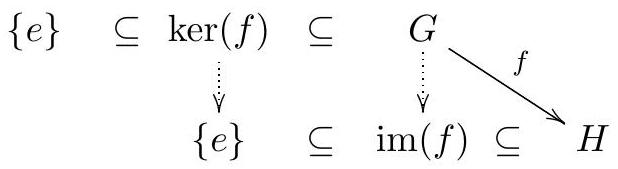
\includegraphics[max width=\textwidth, center]{2025_06_13_6ba93caed1e95a95104eg-017}\\
ab. Dabei zeigt Proposition 2.14, daß bezüglich Untergruppen zwischen $\operatorname{ker}(f)$ und $G$ das „gleiche" passiert, wie zwischen $\{e\}$ und $\operatorname{im}(f)$.\\
2.3. Schnitt, Vereinigung und Erzeuger. Untergruppen vertragen sich mit Schnitten.

Lemma 2.17. Sei $G$ eine Gruppe, I eine Menge und für jedes $i \in I$ eine Untergruppe $U_{i} \leq G$ gegeben. Dann ist der Schnitt eine Untergruppe von $G$ :

$$
U=\bigcap_{i \in I} U_{i}=\left\{g \in G ; g \in U_{i} \text { für alle } i \in I\right\} .
$$

Beweis. Wir weisen Proposition 2.7(c) nach. Zuerst enthält jede Untergruppe $U_{i}$ das neutrale Element $e \in G$. Daher ist $e \in U$ und $U$ nicht leer.

Für $u, v \in U$ gilt $u, v \in U_{i}$ für alle $i$. Damit nach Proposition 2.7(c) auch $u v^{-1} \in U_{i}$, und somit $u v^{-1} \in U$. (Hier ist wesentlich, daß das Inverse $v^{-1}$ in allen Untergruppen $U_{i}$ dasselbe Element ist, denn es stimmt mit dem Inversen aus $G$ überein.)

Bemerkung 2.18. Lemma 2.17 funktioniert auch im Fall einer leeren Indexmenge $I=\emptyset$. Die Bedingung $g \in U_{i}$ für alle $i \in I$ ist dann eine leere Bedingung, denn es gibt keine Untergruppe, die das Element $g$ einschränken könnte. Daher ist in diesem Fall der Schnitt gleich $G$ selbst.

Bei der Vereinigung ist die Situation spezieller.\\
Lemma 2.19. Sei $G$ eine Gruppe, und für jedes $i \in \mathbb{N}$ eine Untergruppe $U_{i} \leq G$ gegeben, so daß diese eine aufsteigende Kette

$$
U_{1} \subseteq U_{2} \subseteq U_{3} \subseteq \ldots \subseteq U_{i} \subseteq U_{i+1} \subseteq \ldots
$$

bilden. Dann ist die Vereinigung eine Untergruppe von $G$ :

$$
U=\bigcup_{i \in \mathbb{N}} U_{i}
$$

Beweis. Wir weisen Proposition 2.7(c) nach. Zuerst ist $U$ nicht leer, denn das neutrale Element von $G$ ist in $U_{i}$ (sogar für jedes $i$ ).

Für $u, v \in U$ gibt es $i, j \in \mathbb{N}$ mit $u \in U_{i}$ und $v \in U_{j}$. Wenn $k \geq \max \{i, j\}$, dann ist $u, v \in U_{k}$, also $u v \in U_{k} \subseteq U$ und $u^{-1} \in U_{k} \subseteq U$.

Definition 2.20. Sei $G$ eine Gruppe und $S \subseteq G$ eine Teilmenge. Die von $S$ erzeugte Untergruppe $\langle S\rangle \subseteq G$ ist definiert über die folgenden zwei Eigenschaften:\\
(i) $\langle S\rangle \subseteq G$ ist eine Untergruppe von $G$, die $S$ enthält,\\
(ii) jede Untergruppe $U \subseteq G$ mit $S \subseteq U$, enthält auch $\langle S\rangle$.

Die Elemente von $S$ heißen Erzeuger von $\langle S\rangle$.\\
Sei $T \subseteq G$ eine Teilmenge. Wir definieren $T^{0}=\{1\}$ und für alle $n \geq 1$ rekursiv

$$
T^{n}:=T \cdot T^{n-1}=\left\{t_{1} \cdot \ldots \cdot t_{n} ; t_{i} \in T \text { für alle } i=1, \ldots, n\right\}=\underbrace{T \cdot \ldots \cdot T}_{n \text {-mal }} \text {. }
$$

Proposition 2.21. Sei $G$ eine Gruppe und $S \subseteq G$ eine Teilmenge. Dann ist $\langle S\rangle$ wohldefiniert und hat die folgenden zwei Beschreibungen (mit $T=S \cup S^{-1}$ ):

$$
\langle S\rangle=\bigcap_{S \subseteq U, U \subseteq G \text { Untergrp. }} U=\bigcup_{n \geq 0} T^{n}
$$

Beweis. Wir müssen zeigen, daß es eine Untergruppe $\langle S\rangle$ mit den in der Definition geforderten Eigenschaften gibt. Sei

$$
H=\bigcap_{S \subseteq U, U \subseteq G \text { Untergrp. }} U
$$

Der Schnitt $H$ ist als Schnitt von Untergruppen nach Lemma 2.17 selbst eine Untergruppe. Offensichtlich gilt $S \subseteq H$. Es ist über jede Untergruppe $U$, die $S$ enthält, zu schneiden, also gilt $H \subseteq U$. Damit erfüllt $H$ die Forderungen für $\langle S\rangle$.

Angenommen, $H$ und $H^{\prime}$ erfüllen die Forderungen aus Definition 2.20. Dann ist $S \subseteq H$ wegen (i), und somit folgt aus (ii) auch $H^{\prime} \subseteq H$. Gleiches gilt mit vertauschten Rollen, also $H=H^{\prime}$. Die Gruppe $\langle S\rangle$ ist somit eindeutig durch (i) und (ii) beschrieben.

Wir zeigen nun die zweite Beschreibung. Die Menge

$$
H=\bigcup_{n \geq 0} T^{n}
$$

ist nicht leer (wegen der Konvention für $T^{0}$ ) und abgeschlossen unter der Gruppenverknüpfung

$$
T^{n} \cdot T^{m}=T^{n+m}
$$

Da $T=S \cup S^{-1}=\left(S^{-1} \cup S\right)^{-1}=T^{-1}$ und

$$
\left(g_{1} \cdot \ldots \cdot g_{n}\right)^{-1}=g_{n}^{-1} \cdot \ldots \cdot g_{1}^{-1}
$$

ist $\left(T^{n}\right)^{-1} \subseteq T^{n}$ und $H$ auch abgeschlossen unter Inversenbildung. Damit ist $H$ nach Proposition 2.7 eine Untergruppe. Die Forderungen (i) und (ii) aus Definition 2.20 sind von $H$ offensichtlich erfüllt. Aufgrund der Eindeutigkeit gilt dann auch $H=\langle S\rangle$.

Definition 2.22. Ein Erzeugendensystem für eine Gruppe $G$ ist eine Teilmenge $S \subseteq G$ mit

$$
\langle S\rangle=G
$$

Kann man für $G$ eine endliche Menge $S$ finden mit $G=\langle S\rangle$, dann nennt man $G$ endlich erzeugt.

Beispiel 2.23. (1) Sei $n \in \mathbb{Z}$. Dann ist $\langle n\rangle=n \mathbb{Z}$.\\
(2) Wir betrachten nun die Menge $S=\{15,21\}$ in der Gruppe $\mathbb{Z}$. Die Gruppe $\langle 15,21\rangle$ enthält auch

$$
6=21-15
$$

und daher

$$
3=15-6-6
$$

Wegen $3 \in\langle 15,21\rangle$ folgt

$$
3 \mathbb{Z}=\langle 3\rangle \subseteq\langle 15,21\rangle \subseteq 3 \mathbb{Z}
$$

also Gleichheit $\langle 15,21\rangle=3 \mathbb{Z}$. Die vorgeführte Rechnung ist nichts anderes als der euklidische Algorithmus, siehe Kapitel 10.2.\\
(3) Allgemeiner gibt es zu $a_{1}, \ldots, a_{n} \in \mathbb{Z}$ nach Satz 2.8 ein eindeutiges $d \geq 0$ mit

$$
\left\langle a_{1}, \ldots, a_{n}\right\rangle=d \mathbb{Z}
$$

Dieses $d$ ist der größte gemeinsame Teiler der $a_{1}, \ldots, a_{n}$, siehe Kapitel 10.1.\\
(4) In der Theorie der Determinante nutzt man aus, daß die Antisymmetrie bezüglich Vertauschung von Spalten zur allgemeinen Symmetrie mit Vorzeichen durch sign( $\sigma$ ) für beliebige Elemente $\sigma \in S_{n}$ der symmetrischen Gruppe führt. Das begründet man damit, daß man jede Permutation als Komposition von Zweiervertauschungen (Transpositionen) schreiben kann (man denke an den Sortieralgorithmus Bubblesort). Die Menge der Transpositionen in $S_{n}$ ist ein Erzeugendensystem von $S_{n}$.

Beispiel 2.24. Der klassische Rubik's Cube mit der Kantenlänge aus 3 Elementarwürfeln hat auf seinen 6 Flächen insgesamt $6 \cdot 3^{2}=54$ Farbkacheln. Als Spielzug kann man eine Vierteldrehung einer jeder der 6 Seitenflächen des Würfels ausführen (eine Drehung einer Mittelebene entspricht der Drehung beider dazu parallelen Seitenfächen in die entgegengesetzte Richtung). Ein solcher Spielzug permutiert die 54 Farbkacheln auf eine charakteristische Weise: jeder Spielzug entspricht einer Permutation in $S_{54}$. Wir definieren, jeweils als Vierteldrehung im Uhrzeigersinn (bei Beobachtungsrichtung von Außen auf die entsprechende Seite), der Seitenflächen L(inks), R(echts), V(orne), H(inten), O(ben) und U(unten) Elemente

$$
L, R, V, H, O, U \in S_{54}
$$

Die Inversen Permutationen

$$
L^{-1}, R^{-1}, V^{-1}, H^{-1}, O^{-1}, U^{-1} \in S_{54}
$$

entsprechen den Vierteldrehungen um die jeweilige Seitenfläche in Richtung entgegen dem Uhrzeigersinn. Die Gruppe des $3 \times 3 \times 3$ Rubik's Cube ist

$$
\mathscr{R}_{3}:=\langle L, R, V, H, O, U\rangle \subseteq S_{54}
$$

Jede Abfolge von Spielzügen hat einen Effekt auf die 54 Farbkacheln, der durch ein Gruppenelement aus $\mathscr{R}_{3}$ beschrieben wird. Ein den Regeln entsprechend verdrehter Würfel entspricht einem Element $g \in \mathscr{R}_{3}$, welcher die Züge in aufmultiplizierter Form enthält, die bei der Verdrehung aus dem gelösten Originalzustand benutzt wurden. Eine Lösung entsteht durch eine Abfolge von Drehungen

$$
X_{1}, \ldots, X_{n}
$$

mit für alle $i=1, \ldots, n$

$$
X_{i} \in\left\{L, R, V, H, O, U, L^{-1}, R^{-1}, V^{-1}, H^{-1}, O^{-1}, U^{-1}\right\}
$$

so daß

$$
X_{n} X_{n-1} \cdots X_{1} g=\mathrm{id} \in S_{54}
$$

das neutrale Element wird.\\
Die Anzahl der Stellungen, in die man einen klassische Rubik's Cube verdrehen kann ist nichts anderes als die Ordnung

$$
\left|\mathscr{R}_{3}\right| .
$$

Die Beschreibung von $\mathscr{R}_{3}$ als Untergruppe von $S_{54}$ ist noch relativ grob. So berücksichtigen wir nicht die Geometrie des Problems: es gibt Mitten-, Kanten-, und Eckwürfel, die von den Spielzügen in ebensolche transformiert werden, und die Farbkacheln in Blöcken zu 1, 2 und 3 beieinander halten. Eine präzisere Beschreibung erlaubt die Bestimmung der Ordnung von $\mathscr{R}_{3}$.

Bemerkung 2.25. Ist zu einer Gruppe $G$ ein Erzeugendensystem $S \subseteq G$ gegeben, dann stellt sich als nächstes die Frage nach einer vollständigen Liste von Relationen, das ist eine ausreichende Liste von Wörtern aus $T=S \cup S^{-1}$, die in $G$ alle zum neutralen Element verknüpfen und erklären können, wenn zwei Wörter in $G$ zum gleichen Element komponieren.

Hier treffen wir auf das Wortproblem, das da fragt, ob ein Wort im Alphabet $T=S \cup S^{-1}$ mittels einer Liste von Relationen $R$ als zum trivialen Element in $G$ komponierend erkannt\\
werden kann. Im Jahr 1952 wurde von Nowikow ${ }^{7}$ (und unabhängig davon von Boone) bewiesen, daß das Wortproblem keine algorithmische Lösung erlaubt.

Das Verständnis von Gruppen muß also auf einem anderen Wege angestrebt werden.\\
Proposition 2.26. Sei $f: G \rightarrow H$ ein Gruppenhomorphismus und $S \subseteq G$ eine Teilmenge.\\
Dann ist

$$
f(\langle S\rangle)=\langle f(S)\rangle .
$$

Beweis. Das ist trivial in der Beschreibung $\langle S\rangle=\bigcup_{n \geq 0} T^{n}$ mit $T=S \cup S^{-1}$ :

$$
f(T)=f(S) \cup f(S)^{-1}, \quad f\left(T^{n}\right)=(f(T))^{n}
$$

\section*{Übungsaufgaben zu §2}
Übungsaufgabe 2.1 (Quaternionen). Sei $\mathbb{H} \subseteq \mathrm{M}_{2}(\mathbb{C})$ die Menge der Matrizen

$$
\left(\begin{array}{cc}
z & -\bar{w} \\
w & \bar{z}
\end{array}\right)
$$

mit $z, w \in \mathbb{C}$ beliebig. Zeigen Sie, daß $\mathbb{H}^{\times}=\mathbb{H} \backslash\{0\}$ eine Untergruppe von $\mathrm{GL}_{2}(\mathbb{C})$ ist.\\
Übungsaufgabe 2.2 (Quaternionengruppe). Wir betrachten die Teilmenge $\mathbb{Q}_{8} \subseteq \mathbb{H}^{\times}$derjenigen Quaternionen

$$
\left(\begin{array}{cc}
z & -\bar{w} \\
w & \bar{z}
\end{array}\right)
$$

mit $z=0$ und $w \in\{ \pm 1, \pm i\}$ oder $w=0$ und $z \in\{ \pm 1, \pm i\}$. Zeigen Sie, daß $Q_{8}$ eine Untergruppe aus 8 Elementen ist, die von Elementen

$$
i:=\left(\begin{array}{cc}
i & \\
& -i
\end{array}\right), \quad j:=\left(\begin{array}{ll} 
& 1 \\
-1 &
\end{array}\right), \quad k:=\left(\begin{array}{ll} 
& i \\
i &
\end{array}\right) .
$$

erzeugt wird, wobei

$$
i^{2}=j^{2}=k^{2}=\left(\begin{array}{ll}
-1 & \\
& -1
\end{array}\right)
$$

und

$$
i j=k
$$

Bestimmen Sie die Ordnung der Elemente von $Q_{8}$.\\
Übungsaufgabe 2.3. Sei $G=G_{1} \times G_{2}$ das Produkt zweier Gruppen $G_{1}$ und $G_{2}$. Zeigen Sie, daß

$$
Z(G)=Z\left(G_{1}\right) \times Z\left(G_{2}\right) .
$$

Übungsaufgabe 2.4. Sei $n \geq 1$ eine natürliche Zahl und $K$ ein Körper. Bestimmen Sie das Zentrum von $\mathrm{GL}_{n}(K)$.

Übungsaufgabe 2.5. Sei $n \geq 1$. Wir definieren die Abbildung $(-)^{\dagger}: \mathrm{GL}_{n}(K) \rightarrow \mathrm{GL}_{n}(K)$ durch

$$
A^{\dagger}:=\left(A^{-1}\right)^{t}
$$

Zeigen Sie, daß es sich um einen Automorphismus von $\mathrm{GL}_{n}(K)$ handelt und bestimmen Sie seine Ordnung als Element von $\operatorname{Aut}\left(\operatorname{GL}_{n}(K)\right)$.

\footnotetext{${ }^{7}$ Pjotr Sergejewitsch Nowikow, 1901-1975, russischer Mathematiker.
}Übungsaufgabe 2.6. Unter $\mathrm{SL}_{2}(\mathbb{Z})$ verstehen wir die Teilmenge von $\mathrm{SL}_{2}(\mathbb{R})$ bestehend aus Matrizen mit Einträgen aus $\mathbb{Z}$ :

$$
\mathrm{SL}_{2}(\mathbb{Z})=\left\{A=\left(\begin{array}{ll}
a & b \\
c & d
\end{array}\right) ; \operatorname{det}(A)=1, a, b, c, d \in \mathbb{Z}\right\}
$$

Zeigen Sie, daß $\mathrm{SL}_{2}(\mathbb{Z})$ eine Untergruppe ist und von den beiden Matrizen

$$
\left(\begin{array}{ll}
1 & 1 \\
0 & 1
\end{array}\right) \quad\left(\begin{array}{ll}
1 & 0 \\
1 & 1
\end{array}\right)
$$

erzeugt wird.\\
Übungsaufgabe 2.7. Seien $f_{1}: G_{1} \rightarrow H$ und $f_{2}: G_{2} \rightarrow H$ Gruppenhomomorphismen. Das Faserprodukt von $G_{1}$ und $G_{2}$ über $H$ (entlang der Gruppenhomomorphismen $f_{1}$ und $f_{2}$ ) ist die Untergruppe von $G_{1} \times G_{2}$ gegeben durch

$$
G_{1} \times_{H} G_{2}:=\left\{\left(g_{1}, g_{2}\right) \in G_{1} \times G_{2} ; f_{1}\left(g_{1}\right)=f_{2}\left(g_{2}\right)\right\}
$$

(a) Zeigen Sie, daß $G_{1} \times H G_{2}$ wie behauptet eine Untergruppe von $G_{1} \times G_{2}$ ist.\\
(b) Zeigen Sie, daß die Projektionen pr ${ }_{i}: G_{1} \times{ }_{H} G_{2} \rightarrow G_{i}$ definiert durch $\operatorname{pr}_{i}\left(g_{1}, g_{2}\right)=g_{i}$ Gruppenhomomorphismen sind.\\
(c) Sei $T$ eine Gruppe und seien $\varphi_{i}: T \rightarrow G_{i}$ für $i=1,2$ Gruppenhomomorphismen mit $f_{1} \circ \varphi_{1}=f_{2} \circ \varphi_{2}$ als Gruppenhomomorphismen $T \rightarrow H$. Zeigen Sie, daß es genau einen Gruppenhomomorphismus $\varphi: T \rightarrow G_{1} \times H G_{2}$ gibt mit $\varphi_{i}=\operatorname{pr}_{i} \circ \varphi$ für $i=1,2$.

Übungsaufgabe 2.8. Sei $n \geq 1$ und sei $K$ ein Körper. Zeigen Sie, daß die Menge aller Elementarmatrizen $E_{i j}(\alpha)$ (auf der Diagonale 1 und genau ein von Null verschiedener Eintrag $\alpha$ abseits der Diagonale an Position $(i, j))$ mit $i \neq j$ die Gruppe $\operatorname{SL}_{n}(K)$ erzeugt.

Tipp: Denken Sie an das Gaußsche Eliminationsverfahren. Des weiteren ist die folgenden Rechnungen hilfreich

$$
\begin{aligned}
& \left(\begin{array}{ll}
1 & a \\
0 & 1
\end{array}\right)\left(\begin{array}{cc}
1 & 0 \\
-a^{-1} & 1
\end{array}\right)\left(\begin{array}{ll}
1 & a \\
0 & 1
\end{array}\right)=\left(\begin{array}{cc}
0 & a \\
-a^{-1} & 0
\end{array}\right) \\
& \left(\begin{array}{cc}
0 & a \\
-a^{-1} & 0
\end{array}\right)\left(\begin{array}{cc}
0 & b \\
-b^{-1} & 0
\end{array}\right)=\left(\begin{array}{cc}
-a / b & \\
& -b / a
\end{array}\right)
\end{aligned}
$$

\section*{Ordnung und zyklische Gruppen}
In diesem Kapitel betrachten wir Potenzen eines Gruppenelements. Dies führt zum Begriff der Ordnung des Elements und der vom Element erzeugten Untergruppe.\\
3.1. Die Potenzen eines Elements. In multiplikativer Schreibweise kann man Gruppenelemente potenzieren.

Definition 3.1. Sei $g \in G$ ein Element einer Gruppe $G$ mit neutralem Element 1. Wir setzen $g^{0}=1$ und dann für $n \geq 1$ rekursiv

$$
\begin{aligned}
g^{n} & =g^{n-1} \cdot g \\
g^{-n} & =g^{-(n-1)} \cdot g^{-1}
\end{aligned}
$$

Die Notation $g^{-1}$ ist doppelt, aber konsistent definiert. Für $n \geq 1$ ergibt sich

$$
g^{n}=\underbrace{g \cdot \ldots \cdot g}_{n \text {-mal }} \quad \text { und } \quad g^{-n}=\underbrace{g^{-1} \cdot \ldots \cdot g^{-1}}_{n \text {-mal }}
$$

Lemma 3.2. Sei $g \in G$ ein Gruppenelement. Für alle $n \in \mathbb{Z}$ gilt

$$
g^{n+1}=g^{n} \cdot g
$$

Beweis. Für $n \geq 0$ gilt dies per Definition. Für $n<0$ setzen wir $n=-m$ mit $m>0$ und rechnen

$$
g^{n+1}=g^{-(m-1)}=g^{-(m-1)} \cdot\left(g^{-1} \cdot g\right)=\left(g^{-(m-1)} \cdot g^{-1}\right) \cdot g=g^{-m} \cdot g=g^{n} \cdot g
$$

Die üblichen Potenzregeln mit fester Basis gelten, denn diese spiegeln nur die Abzählkombinatorik von Faktoren wider.

Proposition 3.3 (Potenzgesetze). Sei $g \in G$ ein Gruppenelement und $n, m \in \mathbb{Z}$. Dann gelten\\
(1) $g^{0}=1$ und $g^{1}=g$,\\
(2) $g^{n} \cdot g^{m}=g^{n+m}$,\\
(3) $g^{-n}=\left(g^{n}\right)^{-1}$,\\
(4) $\left(g^{n}\right)^{m}=g^{n m}$.

Beweis. Das ist trivial. Formal gelingt der Beweis am besten durch Fallunterscheidung nach den Vorzeichen von $n$ und $m$ sowie durch vollständige Induktion. Die Aussage (1) folgt direkt aus der Definition.

Wir beweisen (2) per Induktion nach $|m|$. Der Induktionsanfang hat $m=0$ und gilt trivialerweise: $g^{n} \cdot g^{0}=g^{n} \cdot 1=g^{n}=g^{n+0}$. Wir nehmen nun an, daß (2) in allen Fällen mit kleinerem $|m|$ gilt. Es gibt nun zwei Fälle je nach Vorzeichen von $m$ :

\begin{itemize}
  \item $m \geq 1$. Wir verwenden die Induktionsannahme für $n$ und $m-1$ :
\end{itemize}

$$
g^{n} \cdot g^{m-1}=g^{n+m-1}
$$

Dann rechnen wir mit Lemma 3.2

$$
g^{n} \cdot g^{m}=g^{n} \cdot\left(g^{m-1} \cdot g\right)=\left(g^{n} \cdot g^{m-1}\right) \cdot g=g^{n+m-1} \cdot g=g^{n+m}
$$

\begin{itemize}
  \item $m \leq-1$. Wir verwenden die Induktionsannahme für $n$ und $m+1$ :
\end{itemize}

$$
g^{n} \cdot g^{m+1}=g^{n+m+1}
$$

Dann rechnen wir mit Lemma 3.2

$$
\left(g^{n} \cdot g^{m}\right) \cdot g=g^{n} \cdot\left(g^{m} \cdot g\right)=g^{n} \cdot g^{m+1}=g^{n+m+1}=g^{n+m} \cdot g
$$

Durch Multiplikation mit $g^{-1}$ von rechts ergibt sich die Behauptung.\\
Jetzt beweisen wir (3). Nach Proposition 1.13 reicht die Rechnung (mittels (2))

$$
g^{-n} \cdot g^{n}=g^{-n+n}=g^{0}=1
$$

Aussage (4) beweisen wir zunächst per Induktion nach $m$ für $m \geq 0$. Der Fall $m=0$ ist trivial und die Rechnung

$$
\left(g^{n}\right)^{m+1}=\left(g^{n}\right)^{m} \cdot g^{n}=g^{n m} \cdot g^{n}=g^{n m+n}=g^{n(m+1)}
$$

zeigt den Induktionsschritt.\\
Der Fall $m<0$ wird durch zweimaliges Anwenden von (3) auf den Fall $m>0$ zurückgeführt:

$$
\left(g^{n}\right)^{m}=\left(\left(g^{n}\right)^{-m}\right)^{-1}=\left(g^{-n m}\right)^{-1}=g^{n m}
$$

Korollar 3.4. Sei $G$ eine Gruppe und $g \in G$ ein Element. Die Abbildung

$$
\varphi: \mathbb{Z} \rightarrow G, \quad \varphi(a)=g^{a}
$$

ist ein Gruppenhomomorphismus.\\
Beweis. Das ist genau das Potenzgesetz $\varphi(n+m)=g^{n+m}=g^{n} \cdot g^{m}=\varphi(n) \varphi(m)$ von Proposition 3.3 (2).

Bemerkung 3.5. Man beachte hingegen, daß in der Regel für $g, h \in G$ und $n \in \mathbb{Z}$

$$
(g h)^{n} \neq g^{n} h^{n}
$$

Per Induktion nach $n$ zeigt man: aus $g h=h g$ folgt $(g h)^{n}=g^{n} h^{n}$ für alle $n \in \mathbb{Z}$.

Bemerkung 3.6. In einer abelschen Gruppe $A$ verwenden wir für $a \in A$ und $n \in \mathbb{Z}$ anstelle der Potenzschreibweise $a^{n}$ die additive Notation

$$
n a:=a^{n} .
$$

Damit ist für $n \geq 1$

$$
n a=\underbrace{a+\ldots+a}_{n \text {-mal }} \quad \text { und } \quad(-n) a=\underbrace{(-a)+\ldots+(-a)}_{n \text {-mal }}
$$

In der Notation halten wir uns an Punkt- vor Strichrechnung und sparen so Klammern.\\
Proposition 3.3 übersetzt sich in die erwarteten Assoziativ- und Distributivgesetze: für alle $a, b \in A$ und $n, m \in \mathbb{Z}$ gilt

$$
\begin{aligned}
(n \cdot m) a & =n(m a) \\
(-n) a & =-(n a) \\
(n+m) a & =n a+m a
\end{aligned}
$$

Da $A$ kommutativ ist, gilt zudem auch noch das andere Distributivgesetz

$$
n(a+b)=n a+n b
$$

3.2. Die Ordnung. Die Ordnung eines Elements $g$ gibt Auskunft über die Periode der Wiederholungen in der Folge $\left(g^{n}\right)_{n \geq 0}$ der Potenzen.\\
Definition 3.7. Die Ordnung eines Elements $g$ einer Gruppe $G$ ist

$$
\operatorname{ord}(g):= \begin{cases}\min \left\{n \in \mathbb{N}, n>0 ; g^{n}=1\right\} & \text { falls es ein } n>0 \text { gibt mit } g^{n}=1 \\ \infty & \text { sonst. }\end{cases}
$$

Wenn ord $(g)=\infty$ gilt, so hat $g$ unendliche Ordnung, andernfalls hat $g$ endliche Ordnung.\\
Beispiel 3.8. (1) Betrachten wir das Element $1 \in \mathbb{Z}$. Dann ist für $n \in \mathbb{Z}$

$$
n \cdot 1=n
$$

also hat 1 unendliche Ordnung: ord $(1)=\infty$.\\
(2) Betrachten wir das Element $[1] \in \mathbb{Z} / n \mathbb{Z}$. Dann ist für alle $m \in \mathbb{Z}$

$$
m \cdot[1]=[m]
$$

also ord $([1])=n$.\\
(3) Betrachten wir das Element $\sigma \in S_{n}$, das die Elemente $1,2, \ldots, n$ zyklisch permutiert:

$$
\sigma(i) \equiv i+1 \quad(\bmod n)
$$

oder als Permutation in Form einer Wertetabelle:

$$
\sigma=\left(\begin{array}{ccccc}
1 & 2 & \cdots & n-1 & n \\
2 & 3 & \cdots & n & 1
\end{array}\right)
$$

Dann gilt für alle $i \in\{1, \ldots, n\}$

$$
\sigma^{r}(i) \equiv i+r \quad(\bmod n)
$$

und somit ord $(\sigma)=n$.\\
(4) Für $\varphi \in \mathbb{R}$ betrachte die Matrix

$$
D_{\varphi}=\left(\begin{array}{rr}
\cos (\varphi) & -\sin (\varphi) \\
\sin (\varphi) & \cos (\varphi)
\end{array}\right)
$$

in $\mathrm{GL}_{2}(\mathbb{R})$, welche eine Drehung um den Winkel $\varphi$ beschreibt. Die Additionstheoreme für Sinus und Cosinus sind gerade äquivalent zur Matrixgleichung

$$
D_{\varphi} D_{\psi}=D_{\varphi+\psi}
$$

Die Zuordnung $\varphi \mapsto D_{\varphi}$ beschreibt daher einen Gruppenhomomorphismus

$$
(\mathbb{R},+) \rightarrow \mathrm{GL}_{2}(\mathbb{R})
$$

Sei $n \in \mathbb{N}$ und speziell $\varphi=\frac{2 \pi}{n}$. Dann ist in $\mathrm{GL}_{2}(\mathbb{R})$

$$
\left(D_{2 \pi / n}\right)^{n}=D_{2 \pi}=\left(\begin{array}{ll}
1 & 0 \\
0 & 1
\end{array}\right)
$$

aber $\left(D_{2 \pi / n}\right)^{m}=D_{2 \pi m / n} \neq\left(\begin{array}{ll}1 & 0 \\ 0 & 1\end{array}\right)$ für alle $0<m<n$. Das Element $D_{2 \pi / n}$ hat also die Ordnung $n$.\\
(5) Sei $K$ ein Körper und $A \in \mathrm{GL}_{n}(K)$ die Matrix (der Rest wird mit 0 aufgefüllt)

$$
A=\left(\begin{array}{llll} 
& & & 1 \\
1 & & & \\
& \ddots & & \\
& & 1 &
\end{array}\right)
$$

Dies beschreibt die lineare Abbildung, welche auf der Standardbasis ( $e_{1}, \ldots, e_{n}$ ) durch

$$
A e_{i}=e_{i+1}
$$

(mit dem Index modulo $n$ ) wirkt. Es gilt

$$
\operatorname{ord}(A)=n
$$

wie man aus $A^{r} e_{i}=e_{i+r}$ (mit dem Index modulo $n$ ) sofort sieht.\\
Der Beweis von Satz 2.8 über die Klassifikation der Untergruppen von $\mathbb{Z}$ übersetzt sich in die folgende Charakterisierung der Ordnung eines Elements.

Proposition 3.9. Sei $G$ eine Gruppe und $g \in G$ ein Element. Sei $\varphi: \mathbb{Z} \rightarrow G$ die Abbildung $\varphi(a)=g^{a}$ aus Korollar 3.4. Dann gilt

$$
\operatorname{ker}(\varphi)= \begin{cases}\operatorname{ord}(g) \mathbb{Z} & \text { falls g endliche Ordnung hat, } \\ \{0\} & \text { falls g unendliche Ordnung hat. }\end{cases}
$$

Beweis. Der $\operatorname{Kern} \operatorname{ker}(\varphi)$ ist eine Untergruppe von $\mathbb{Z}$. Als solche hat $\operatorname{ker}(\varphi)$ die Form $n \mathbb{Z}$ für ein eindeutiges $n \geq 0$. Dieser Erzeuger wird im Beweis von Satz 2.8 genau so bestimmt, wie in Definition 3.7 die Ordnung von $g$ im endlichen Fall:

$$
n \in \operatorname{ker}(\varphi) \Longleftrightarrow \varphi(n)=1 \Longleftrightarrow g^{n}=1
$$

Korollar 3.10. Sei $g \in G$ und $m \in \mathbb{Z}$ mit $g^{m}=1$. Dann ist $m=0$, wenn ord $(g)=\infty$, oder ein Vielfaches der Ordnung ord $(g)$, wenn $g$ endliche Ordnung hat.

Beweis. Das folgt sofort aus der Beschreibung von $\operatorname{ker}(\varphi)$ im Beweis von Proposition 3.9.\\
Korollar 3.11. Sei $g \in G$ ein Element endlicher Ordnung ord $(g)=n$. Dann gilt

$$
g^{a}=g^{b} \Longleftrightarrow a \equiv b \quad(\bmod n)
$$

Beweis. Wegen $g^{a-b}=g^{a} \cdot\left(g^{b}\right)^{-1}=1$ folgt $a-b \in \operatorname{ker}(\varphi)$ mit $\varphi$ wie in Proposition 3.9. Aus $\operatorname{ker}(\varphi)=n \mathbb{Z}$ folgt die Behauptung.

Bemerkung 3.12. Sei $G$ eine Gruppe und $g \in G$ ein Element. Das Bild der Abbildung $\varphi(a)=g^{a}$ aus Korollar 3.4 besteht aus den Potenzen von $g$. Nach Proposition 2.21 ist dies auch genau die von $g$ in $G$ erzeugte Untergruppe. Damit gilt

$$
\langle g\rangle=\operatorname{im}(\varphi)=\left\{g^{a} ; a \in \mathbb{Z}\right\}
$$

Definition 3.13. Die Ordnung einer Gruppe $G$ ist die Mächtigkeit (die Anzahl der Elemente)\\
der zugrundeliegenden Menge $G$.\\
Beispiel 3.14. (1) Die Gruppe $\mathbb{Z} / n \mathbb{Z}$ hat die Ordnung

$$
|\mathbb{Z} / n \mathbb{Z}|=n
$$

denn durch $\{0, \ldots, n-1\}$ wird ein vollständiges Vertretersystem für die Äquivalenzklassen modulo $n$ beschrieben.\\
(2) Sind $G$ und $H$ endliche Gruppen, so ist $G \times H$ endlich und $|G \times H|=|G| \cdot|H|$.

Proposition 3.15 (Zwei Bedeutungen von Ordnung). Sei $G$ eine Gruppe und $g \in G$ ein Element. Dann hat die Untergruppe $\langle g\rangle$ die Ordnung $|\langle g\rangle|=\operatorname{ord}(g)$, genauer gilt:\\
(1) Sei $\operatorname{ord}(g)=n$ endlich. Dann gilt $|\langle g\rangle|=n=\operatorname{ord}(g)$ und

$$
\langle g\rangle=\left\{g^{0}=1, g, g^{2}, \ldots, g^{n-1}\right\}
$$

(2) Sei $\operatorname{ord}(g)=\infty$ unendlich. Dann gilt für alle $a, b \in \mathbb{Z}$, daß aus $g^{a}=g^{b}$ bereits $a=b$ folgt, und $|\langle g\rangle|=\operatorname{ord}(g)$ ist unendlich.

Beweis. (1) Sei ord $(g)=n$ endlich. Mittels Division mit Rest kann man jede ganze Zahl $a$ als $a=q n+r$ mit $0 \leq r<n$ schreiben. Dann ist

$$
g^{a}=g^{q n+r}=\left(g^{n}\right)^{q} \cdot g^{r}=g^{r}
$$

Damit hat $\langle g\rangle$ die angegebenen Elemente. Es bleibt zu zeigen, daß keine zwei $g^{a}$ und $g^{b}$ mit $0 \leq a<b \leq n-1$ gleich sind. Aber aus $g^{a}=g^{b}$ folgt $b-a \in n \mathbb{Z}$ sofort aus Korollar 3.11 und das widerspricht $0<b-a<n$.\\
(2) Angenommen $g^{a}=g^{b}$ mit ganzen Zahlen $a \neq b$. Dann ist oBdA $b>a$ und damit $g^{b-a}=1$ im Widerspruch zur Definition von ord $(g)=\infty$.\\
3.3. Zyklische Gruppen. Die arithmetisch einfachsten Gruppen sind die zyklischen Gruppen.

Definition 3.16. Eine zyklische Gruppe ist eine Gruppe $G$, für die es ein Element $g \in G$ gibt mit

$$
G=\langle g\rangle
$$

Man sagt, $g$ ist ein Erzeuger und $G$ wird von $g$ erzeugt.\\
Beispiel 3.17. Die wichtigsten Beispiele von Erzeugern in Gruppen sind die folgenden.\\
(1) Die Gruppe $\mathbb{Z}$ wird von $1 \in \mathbb{Z}$ erzeugt und ist somit zyklisch. Auch $-1 \in \mathbb{Z}$ ist ein Erzeuger, und es gibt keinen weiteren Erzeuger für $\mathbb{Z}$.\\
(2) Sei $n$ eine natürliche Zahl. Dann ist die Restklasse von 1 in $\mathbb{Z} / n \mathbb{Z}$ ein Erzeuger. Zum Beispiel überlege man sich, daß 1 ein Erzeuger von $\mathbb{Z}$ ist, und wegen des surjektiven Gruppenhomomorphismus $\mathbb{Z} \rightarrow \mathbb{Z} / n \mathbb{Z}$ auch das Bild ein Erzeuger von $\mathbb{Z} / n \mathbb{Z}$. Damit ist

$$
\mathbb{Z} / n \mathbb{Z}
$$

eine zyklische Gruppe, und zwar der Ordnung $n$.\\
(3) Verschiedene Elemente einer Gruppe können diese erzeugen. Zum Beispiel wird $\mathbb{Z} / 3 \mathbb{Z}$ sowohl von der Restklasse [1] als auch von [2] erzeugt.\\
(4) In der Gruppe $G=\mathbb{R}_{>0}$ der positiven reellen Zahlen mit der Multiplikation als Verknüpfung ist für jedes feste $a \neq 1$ jedes $x \in G$ von der Form $x=a^{t}$ für ein geeignetes $t$. Trotzdem ist $\mathbb{R}_{>0}$ nicht zyklisch, denn wir benötigen $t=\log (x) / \log (a)$ und das ist in der Regel nur in $\mathbb{R}$ und nicht in $\mathbb{Z}$. Die Untergruppe $\langle a\rangle$ enthält nur die ganzzahligen Potenzen $a^{n}$ mit $n \in \mathbb{Z}$. Also ist $\langle a\rangle \neq \mathbb{R}_{>0}$.

Satz 3.18 (Struktursatz für zyklische Gruppen). Sei G eine zyklische Gruppe. Dann gilt

$$
G \simeq \begin{cases}\mathbb{Z} / n \mathbb{Z} & \text { wenn }|G|=n \text { endlich ist } \\ \mathbb{Z} & \text { wenn }|G|=\infty\end{cases}
$$

Beweis. Da $G$ zyklisch ist, gibt es $g \in G$ mit $G=\langle g\rangle$. Sei $\varphi: \mathbb{Z} \rightarrow G$ der durch $\varphi(a)=g^{a}$ definierte Gruppenhomomorphismus.

Wenn $\operatorname{ord}(g)=|G|$ unendlich ist, dann ist $\operatorname{ker}(\varphi)=\{0\}$ nach Proposition 3.9, also $\varphi$ injektiv nach Proposition 2.14. Da $\varphi$ sowieso surjektiv ist, handelt es sich bei $\varphi$ um einen Isomorphismus.

Sei nun ord $(g)=n$ endlich. Dann definiert nach Korollar 3.11

$$
\bar{\varphi}: \mathbb{Z} / n \mathbb{Z} \rightarrow\langle g\rangle, \quad \bar{\varphi}([a])=g^{a}
$$

eine wohldefinierte Abbildung. Diese ist offensichtlich surjektiv und ebenso nach Korollar 3.11 injektiv. Somit ist $\bar{\varphi}$ der gesuchte Isomorphismus $G \simeq \mathbb{Z} / n \mathbb{Z}$.

Bemerkung 3.19. Satz 3.18 kann man später leichter als Anwendung des Homomorphiesatz, Satz 5.15 bekommen.

Wenn man sich in einer Gruppe nur für die Potenzen eines Elements $g$ interessiert, dann besagt Satz 3.18 angewandt auf $\langle g\rangle$, daß man so tun kann, als ob man in einem der beiden Fälle ist: $\mathbb{Z}$ mit $g=1$ oder $\mathbb{Z} / n \mathbb{Z}$ für ein $n>0$ und $g=[1]$.

Bemerkung 3.20. Sei $p$ eine Primzahl. Die multiplikative Gruppe $\mathbb{F}_{p}^{\times}$des Körpers mit $p$ Elementen ist eine zyklische Gruppe. Dieses erstaunliche und nichttriviale Resultat (uniform in $p$ ) ist ein grundlegendes Ergebnis der elementaren Zahlentheorie. Ein $w \in \mathbb{Z}$, dessen Restklasse $[w] \in \mathbb{F}_{p}^{\times}$ ein Erzeuger ist, wird Primitivwurzel genannt. Zu so einer Primitivwurzel gehört ein Isomorphismus (die Notation ist rein suggestiv und hat nichts mit dem Logarithmus reeller Zahlen zu tun!)

$$
\log _{w}: \mathbb{F}_{p}^{\times} \xrightarrow{\sim} \mathbb{Z} /(p-1) \mathbb{Z}
$$

der durch die Gleichung

$$
w^{\log _{w}(a)} \equiv a \quad(\bmod p) \quad \text { für alle } a \in \mathbb{F}_{p}^{\times}
$$

bestimmt ist. Dieser Isomorphismus wird diskreter Logarithmus genannt, weil er invers zum Exponentialhomomorphismus $n \mapsto w^{n}$ ist. Die Wette, daß $\log _{w}(a)$ teuer zu berechnen ist, bildet die Grundlage für die RSA-Verschlüsselung.\\
3.4. Zykelschreibweise. Zykel sind besonders einfache Elemente der symmetrischen Gruppe.

Definition 3.21. Ein Zykel in der Gruppe $S_{n}$ ist eine Permutation $\sigma \in S_{n}$ der folgenden Form. Es gibt eine Teilmenge, die Trägermenge des Zykels,

$$
A=\left\{a_{1}, \ldots, a_{r}\right\} \subseteq\{1, \ldots, n\}
$$

mit $r \geq 2$ Elementen, so daß $\sigma(b)=b$ für alle $b \notin A$ und

$$
\sigma\left(a_{i}\right)=a_{i+1},
$$

wobei wir die Indizes modulo $r$ betrachten. Die Zahl $r=|A|$ heißt Länge des Zykels, der dann auch $r$-Zykel genannt wird. Eine Transposition ist ein Zykel der Länge 2.

Als Notation verwenden wir

$$
\sigma=\left(a_{1}, a_{2}, \ldots, a_{r}\right)
$$

Haben mehrere Zykel disjunkte Trägermengen, so spricht man von disjunkten Zykeln.\\
Bemerkung 3.22. (1) Man beachte, daß die Elemente der Trägermenge im Zykel nicht der Größe nach geordnet sein müssen. So bildet der Zykel

$$
(1,4,2) \in S_{4}
$$

durch

$$
1 \mapsto 4 \mapsto 2 \mapsto 1 \text { und } 3 \mapsto 3
$$

ab, während

$$
(1,2,4) \in S_{4}
$$

die folgende andere Abbildung darstellt:

$$
1 \mapsto 2 \mapsto 4 \mapsto 1 \text { und } 3 \mapsto 3
$$

(2) Die Notation für einen Zykel ist nicht eindeutig. Für jedes $2 \leq i \leq r$ ist

$$
\left(a_{1}, a_{2}, \ldots, a_{r}\right)=\left(a_{i}, a_{i+1}, \ldots, a_{r}, a_{1}, \ldots, a_{i-1}\right)
$$

als Elemente der symmetrischen Gruppe. Die Reihenfolge der Elemente $a_{i}$ ist wichtig! Aber bei zyklischer Vertauschung beschreiben wir dasselbe Element der $S_{n}$.\\
(3) Nach unserer Definition gibt es keine Zykel der Länge 1. Übertragen wir die Definition sinngemäß auf Zykel der Länge 1, so beschreibt jeder solche die Identität.\\
Proposition 3.23. Für Zykel in $S_{n}$ gelten die folgenden Regeln:\\
(1) $\left(a_{1}, \ldots, a_{r}\right)^{-1}=\left(a_{r}, \ldots, a_{1}\right)$.\\
(2) $\left(a_{1}, a_{2}, \ldots, a_{r}\right)=\left(a_{1}, a_{r}\right) \ldots\left(a_{1}, a_{3}\right)\left(a_{1}, a_{2}\right)$.\\
(3) $\operatorname{sign}\left(\left(a_{1}, a_{2}, \ldots, a_{r}\right)\right)=(-1)^{r-1}$.

Beweis. (1) ist klar. (2) beweisen wir per vollständiger Induktion nach $r \geq 2$. Für $r=2$ ist nichts zu tun. Nehmen wir also an, daß für $r-1$ die Formel bereits gilt. Dann rechnet man sofort

$$
\left(a_{1}, a_{r}\right) \ldots\left(a_{1}, a_{3}\right)\left(a_{1}, a_{2}\right)=\left(a_{1}, a_{r}\right)\left(a_{1}, a_{2}, \ldots, a_{r-1}\right)=\left(a_{1}, a_{2}, \ldots, a_{r}\right)
$$

Aussage (3) folgt sofort aus (2) durch Zählen der Transpositionen im Produkt.\\
Beispiel 3.24. In der $S_{6}$ betrachten wir die Permutation

$$
\sigma=\left(\begin{array}{cccccc}
1 & 2 & 3 & 4 & 5 & 6 \\
6 & 3 & 2 & 1 & 5 & 4
\end{array}\right)
$$

Diese bildet die Elemente $\{1, \ldots, 6\}$ wie folgt ab:

$$
1 \mapsto 6 \mapsto 4 \mapsto 1, \quad 2 \mapsto 3 \mapsto 2, \quad 5 \mapsto 5,
$$

was zu den Zykeln $(1,6,4)$ und $(2,3)$ führt. Man verifiziert sofort

$$
\sigma=(1,6,4)(2,3)=(2,3)(1,6,4)
$$

Proposition 3.25. Für Zykel in $S_{n}$ gelten die folgenden Regeln:\\
(1) Disjunkte Zykel kommutieren miteinander.\\
(2) Ist $\sigma=z_{1} \cdot \ldots \cdot z_{s}$ ein Produkt paarweise disjunkter Zykel $z_{i}$ mit Trägermenge $A_{i}$, dann gilt für alle $i=1, \ldots, s$

$$
\left.\sigma\right|_{A_{i}}=\left.z_{i}\right|_{A_{i}}
$$

und für alle $j \in\{1, \ldots, n\} \backslash \bigcup_{i=1}^{s} A_{i}$ gilt $\sigma(j)=j$.\\
Beweis. (1) Das ist klar: ein Zykel macht nur etwas Nichttriviales auf seiner Trägermenge. Sind diese disjunkt, so kommutieren die entsprechenden zyklischen Permutationen. In Formeln sieht das so aus: seien $\sigma, \pi \in S_{n}$ Permutationen mit disjunkten Trägermenge $A, B \subseteq\{1, \ldots, n\}$, das heißt $\sigma$ ist auf dem Komplement von $A$ die Identität (und folglich $\sigma(A)=A$ ) und $\pi$ ist auf dem Komplement von $B$ die Identität (und folglich $\pi(B)=B$ ). Dann gilt

$$
\sigma \pi(i)=\sigma\left(\left\{\begin{array}{ll}
\pi(i) & i \in B \\
i & i \notin B
\end{array}\right)= \begin{cases}\sigma(i) & i \in A \\
\pi(i) & i \in B \\
i & i \notin A \cup B\end{cases}\right.
$$

und genauso für $\pi \sigma$. Damit gilt $\sigma \pi=\pi \sigma$ wie behauptet.\\
(2) Weil die Trägermengen disjunkt sind, gilt für alle $i \neq j$

$$
\left.z_{j}\right|_{A_{i}}=\operatorname{id}_{A_{i}}
$$

Insbesondere bildet jeder der Zykel $A_{i}$ auf $A_{i}$ ab. Wir können daher rechnen

$$
\left.\sigma\right|_{A_{i}}=\left.\left.z_{1}\right|_{A_{i}} \cdot \ldots z_{s}\right|_{A_{i}}=\left.\operatorname{id}_{A_{i}} \cdot \ldots \cdot z_{i}\right|_{A_{i}} \cdot \ldots \cdot \operatorname{id}_{A_{i}}=\left.z_{i}\right|_{A_{i}}
$$

Beispiel 3.26. Die Elemente $L$ und $R$ aus der Rubik's Cube Gruppe $\mathscr{R}_{3}$ (bzw. analog die Paare $U, O$ und $V, H)$ bestehen aus Produkten von Zykeln deren Träger disjunkt sind: die von $L$ sind in der linken Seitenfläche, die von $R$ in der rechten Seitenfläche. Daher kommutieren $L$ und $R$ :

$$
L R=R L .
$$

Satz 3.27. Jede Permutation $\sigma \in S_{n}$ ist ein Produkt $\sigma=z_{1} \cdot \ldots \cdot z_{s}$ von disjunkten Zykeln, und zwar eindeutig bis auf die Reihenfolge der Zykel. Die Vereinigung der Träger der $z_{i}$ ist das Komplement der Fixpunktmenge $\{j ; \sigma(j)=j\}$ von $\sigma$.\\
Beweis. Das beweisen wir per Induktion nach $N(\sigma)=n-|\{j ; \sigma(j)=j\}|$. Wenn $N(\sigma)=0$ ist, dann handelt es sich um $\sigma=\mathrm{id}$, und es ist nichts zu tun.

Sei $N(\sigma)>0$. Dann gibt es $a \in\{1, \ldots, n\}$ mit $\sigma(a) \neq a$. Die Folge $a_{k}=\sigma^{k}(a)$

$$
a, \sigma(a), \sigma^{2}(a), \ldots
$$

nimmt nur endlich viele Werte an, und mindestens 2. Daher gibt es $r>s \geq 0$ mit $\sigma^{r}(a)=\sigma^{s}(a)$. Wenden wir $\sigma^{-s}$ darauf an, so finden wir $a=\sigma^{r-s}(a)$. Sind $s, r$ minimal gewählt, dann folgt $s=0$ und $r \geq 1$ und

$$
A:=\left\{a_{0}=a, a_{1}, \ldots, a_{r-1}\right\}
$$

ist eine Teilmenge von $\{1, \ldots, n\}$ der Mächtigkeit $r$. Sei $z_{1}$ der Zykel

$$
z_{1}=\left(a_{0}, a_{1}, \ldots, a_{r-1}\right)
$$

Dann ist per Konstruktion $\left.\sigma\right|_{A}=\left.z_{1}\right|_{A}$. Sei $B=\{i ; i \notin A\}$ das Komplement von $A$ in $\{1, \ldots, n\}$, und sei $\sigma_{B} \in S_{n}$ definiert durch

$$
\sigma_{B}(i)= \begin{cases}\sigma(i) & i \in B \\ i & i \in A\end{cases}
$$

Es gilt offensichtlich

$$
\sigma=z_{1} \sigma_{B}
$$

und $N\left(\sigma_{B}\right)=N(\sigma)-r$, weil $\sigma_{B}$ sich auf $B$ wie $\sigma$, hingegen auf $A$ wie die Identität verhält. Per Induktionsvoraussetzung gilt der Satz für $\sigma_{B}$. Es gibt also disjunkte Zykel $z_{2}, \ldots, z_{s}$ mit

$$
\sigma_{B}=z_{2} \cdot \ldots \cdot z_{s}
$$

und die Träger der $z_{i}, i \geq 2$ sind enthalten in $B$. Weil der Träger von $z_{1}$ in $A$ liegt, haben die Zykel $z_{1}, \ldots, z_{s}$ disjunkte Träger und

$$
\sigma=z_{1} \sigma_{B}=z_{1} \cdot z_{2} \cdot \ldots \cdot z_{s}
$$

ist die gesuchte Zerlegung von $\sigma$. Die Behauptung über die Träger folgt sofort aus der Konstruktion oder Proposition 3.25.

Seien $\sigma=z_{1} \cdot \ldots \cdot z_{s}$ und $\sigma=z_{1}^{\prime} \cdot \ldots \cdot z_{t}^{\prime}$ zwei Zerlegungen wie im Satz. Die Eindeutigkeit der Zerlegung in disjunkte Zykel bis auf die Reihenfolge der Faktoren folgt aus Proposition 3.25 (2): demnach sind nämlich die Trägermengen der Zykeln die Äquivalenzklassen der Äquivalenzrelation

$$
i \sim_{\sigma} j: \Longleftrightarrow \text { es gibt } r \in \mathbb{Z} \text { mit } \sigma^{r}(i)=j
$$

Sei $A$ eine dieser Äquivalenzklassen und $z$ bzw. $z^{\prime}$ der entsprechende Faktor in der Produktzerlegung von $\sigma$. Dann gilt weiter nach Proposition 3.25 (2):

$$
z=\left.\sigma\right|_{A}=z^{\prime}
$$

Proposition 3.28. Die Ordnung eines Zykels und eines Elements in Form eines Produkts disjunkter Zykel berechnet sich wie folgt:\\
(1) Ein Zykel der Länge $r$ hat die Ordnung $r$.\\
(2) Sei $\sigma \in S_{n}$ das Produkt von paarweise disjunkten Zykeln der Längen $r_{1}, \ldots, r_{s}$. Dann gilt

$$
\operatorname{ord}(\sigma)=\operatorname{kgV}\left\{r_{1}, r_{2}, \ldots, r_{s}\right\}
$$

Beweis. (1) Sei $\sigma=\left(a_{1}, a_{2}, \ldots, a_{r}\right)$ ein $r$-Zykel. Dann folgt für alle $m \in \mathbb{Z}$

$$
\sigma^{m}\left(a_{i}\right)=a_{i+m}
$$

wobei der Index in $\mathbb{Z} / r \mathbb{Z}$ zu lesen ist. Daher gilt $\sigma^{r}=1$ und $r$ ist minimal in $\mathbb{N}$ mit dieser Eigenschaft.\\
(2) Sei $\sigma=z_{1} \ldots z_{s}$ die Zerlegung in Zykel $z_{i} \in S_{n}$ der Länge $r_{i}$ mit paarweise disjunkten Trägermengen $A_{i}$. Dann kommutieren $z_{i}$ und $z_{j}$ für alle $i, j$ miteinander. Per vollständiger Induktion zeigt man (vgl. Aufgabe 1.4), daß

$$
\sigma^{d}=z_{1}^{d} \ldots z_{s}^{d}
$$

Die Potenz $z_{i}^{d}$ wirkt höchstens auf $A_{i}$ nichttrivial, während $\{1, \ldots, n\} \backslash A_{i}$ punktweise fixiert wird. Es gilt daher $\sigma^{d}=\mathrm{id}$ genau dann, wenn für alle $1 \leq i \leq s$ gilt $z_{i}^{d}=\mathrm{id}$, und damit ist $r_{i}=\operatorname{ord}\left(z_{i}\right)$ ein Teiler von $d$. Daraus folgt sofort die Behauptung.

Beispiel 3.29. Die Elemente $L, R, V, H, O, U$ aus der Rubik's Cube Gruppe $\mathscr{R}_{3}$ haben jeweils eine Darstellung als Produkt von 5 disjunkten 4-Zykeln. Dazu beobachtet man schlicht und einfach, wie sich die Farbkacheln unter einer Vierteldrehung bewegen. Insbesondere gilt für alle $X \in\{L, R, V, H, O, U\}$

$$
\operatorname{sign}(X)=\left((-1)^{3}\right)^{5}=-1
$$

Satz 3.30. Die symmetrische Gruppe $S_{n}$ ist durch Transpositionen erzeugt: jede Permutation ist ein Produkt von Transpositionen.

Beweis. Nach Satz 3.27 reicht es, einen beliebigen Zykel ( $a_{1}, a_{2}, \ldots, a_{r}$ ) als Produkt von Transpositionen zu erzeugen. Dafür liefert Proposition 3.23(2) eine explizite Formel.

\section*{Übungsaufgaben zu §3}
Übungsaufgabe 3.1. Zeigen Sie: eine Gruppe in der jedes nichttriviale Element die Ordnung 2 hat, ist eine abelsche Gruppe.

Übungsaufgabe 3.2. Sei $g$ ein Gruppenelement der Ordnung $n$ und $m \in \mathbb{Z}$. Bestimmen Sie die Ordnung von $g^{m}$.\\
Übungsaufgabe 3.3. Wir betrachten das Quadrat im $\mathbb{R}^{2}$ mit den Ecken $\binom{ \pm 1}{ \pm 1}$. Bestimmen sie die Ordnung der Symmetriegruppe des Quadrats als Untergruppe von $\mathrm{GL}_{2}(\mathbb{R})$.\\
Übungsaufgabe 3.4. Sei $G$ eine Gruppe und $[n]: G \rightarrow G$ für $n \in \mathbb{Z}$ die Abbildung

$$
[n](g)=g^{n}
$$

für alle $g \in G$. Zeigen Sie, daß $[n]$ für alle $n \in \mathbb{Z}$ ein Gruppenhomomorphismus ist genau dann, wenn $G$ abelsch ist.

Übungsaufgabe 3.5. Bestimmen Sie die Ordnung in der Rubik's Cube Gruppe $\mathscr{R}_{3}$ der Elemente\\
(a) $L, R, V, H, O, U$,\\
(b) $\quad V^{-1} R$,\\
(c) $\quad V^{-1} O^{-1} R^{-1} O R V O$.

Beachten Sie, daß $\mathscr{R}_{3}$ als Untergruppe von $S_{54}$ definiert ist und daher die Verknüpfung als Komposition von Bijektionen von rechts nach links fortlaufend auszuführen ist.

Übungsaufgabe 3.6. Beschreiben Sie ein Gegenbeispiel zu folgender Aussage: In einer endlichen Gruppe $G$ gibt es zu jedem Teiler $n||G|$ der Gruppenordnung ein Element $g \in G$ der Ordnung $\operatorname{ord}(g)=n$.

Übungsaufgabe 3.7. Sei $n \geq 1$. Die alternierende Gruppe $A_{n}$ wird von der Menge der 3-Zykel aus $S_{n}$ erzeugt.

\section*{Der Satz von Lagrange}
Mittels des Begriffs der Nebenklasse beweisen wir den Satz von Lagrange als ein erstes Beispiel, daß sich gewisse Eigenschaften einer Gruppe $G$ aus der entsprechenden Eigenschaft einer Untergruppe $U$ und dem noch zu definierenden Quotienten $G / U$ (das ist oft nur eine $G$-Menge, und manchmal selbst eine Gruppe) zusammensetzen lassen.\\
4.1. Nebenklassen. Nebenklassen einer Gruppe $G$ in Bezug auf eine Untergruppe $U$ sind das Analogon zu affinen Unterräumen in Vektorräumen.

Definition 4.1. Sei $U$ eine Untergruppe der Gruppe $G$. Eine Rechtsnebenklasse ist eine Teilmenge von $G$ der Form

$$
U g=\{h \in G ; \text { es gibt ein } u \in U \text { mit } h=u g\}
$$

Eine Linksnebenklasse ist eine Teilmenge der Form

$$
g U=\{h \in G ; \quad \text { es gibt ein } u \in U \text { mit } h=g u\} .
$$

Oft bezeichnet man Rechts- bzw. Linksnebenklassen ungenau einfach als Nebenklasse in der Hoffnung, die Wahl von rechts bzw. links erschließt sich aus dem Kontext.

Proposition 4.2. Sei $f: G \rightarrow H$ ein Gruppenhomomorphismus und $U=\operatorname{ker}(f)$ sein Kern. Dann sind die Nebenklassen in Bezug auf $U$ genau die nichtleeren Urbilder $f^{-1}(h) z u h \in \operatorname{im}(f)$. Insbesondere gilt für alle $g \in G$

$$
g U=f^{-1}(f(g))=U g
$$

d.h. Rechts- und Linksnebenklassen stimmen überein.

Beweis. Es ist $h \in f^{-1}(f(g))$ äquivalent zu $f(h)=f(g)$, und das wiederum ist äquivalent mit $x=g^{-1} h$ zu $f(x)=1$ weil $f(x)=f(g)^{-1} f(h)$. Wegen $h=g x$ bestimmen sich $h$ und $x$ gegenseitig. Somit gilt

$$
f^{-1}(f(g))=\{g x ; f(x)=1\}=g U
$$

Die Variante mit der Rechtsnebenklasse $U g$ folgt genauso.\\
Beispiel 4.3. Hier sind nun ein paar Beispiele für Nebenklassen.\\
(1) Die triviale Nebenklasse ist $U=U e \subseteq G$, wobei $e \in G$ das neutrale Element ist. Es gilt $U e=U=e U$ und daher ist die triviale Nebenklasse sowohl eine Rechts- wie eine Linksnebenklasse.\\
(2) Sei $n \geq 2$. Es ist $A_{n}=\operatorname{ker}\left(\operatorname{sign}: S_{n} \rightarrow\{ \pm 1\}\right.$ der Kern des Signumhomomorphismus. Nach Proposition 4.2 gibt es zwei Nebenklassen, nämlich $A_{n}$ und $S_{n} \backslash A_{n}$ für $U=A_{n}$ in $G=S_{n}$.\\
(3) Sei $U=\left\{\sigma \in S_{n} ; \sigma(1)=1\right\} \simeq S_{n-1}$ in $G=S_{n}$. Dies ist eine Untergruppe, wie später aus der allgemeinen Beschreibung von Stabilisatoruntergruppen sofort folgt. Es gilt nun

$$
g U=\left\{\sigma \in S_{n} ; \sigma(1)=g(1)\right\}
$$

während

$$
U g=\left\{\sigma \in S_{n} ; \sigma^{-1}(1)=g^{-1}(1)\right\}
$$

Diese beiden Nebenklassen sind im Allgemeinen verschieden.

Proposition 4.4. Sei U eine Untergruppe der Gruppe G. Zwei Rechtsnebenklassen sind entweder gleich oder disjunkt: für alle $g, h \in G$ gilt

$$
U g \cap U h \neq \emptyset \quad \Longrightarrow \quad U g=U h
$$

Dieselbe Aussage gilt für Linksnebenklassen.\\
Beweis. Sei $t \in U g \cap U h$. Dann gibt es $u, v \in U$ mit $t=u g=v h$. Aus Symmetriegründen reicht es, die Inklusion $U g \subseteq U h$ zu zeigen. Sei daher $x \in U g$ ein beliebiges Element. Dann gibt es $w \in U$ mit $x=w g$. Die Behauptung folgt nun aus

$$
x=w g=w\left(u^{-1} u\right) g=w u^{-1}(u g)=w u^{-1}(v h)=\left(w u^{-1} v\right) h \in U h .
$$

4.2. Der Index. Nach Proposition 4.4 unterteilt sich eine Gruppe in Bezug auf eine Untergruppe in eine disjunkte Vereinigung von Linksnebenklassen (oder analog Rechtsnebenklassen), indem wir in der Liste aller Linksnebenklassen die Doppelten aussortieren: $\{g U ; g \in G\}$. Dazu gehört die folgende Äquivalenzrelation.

Definition 4.5. Sei $G$ eine Gruppe und $U$ eine Untergruppe. Wir definieren für $x, y \in G$

$$
x \sim_{U}^{r} y \quad: \Longleftrightarrow \quad x \in y U
$$

und sagen dann, daß $x$ zu $y$ modulo $U$ von rechts äquivalent ist. Analog defnieren wir

$$
x \sim_{U}^{l} y \quad: \Longleftrightarrow \quad x \in U y
$$

und sagen, daß $x$ zu $y$ modulo $U$ von links äquivalent ist.\\
Proposition 4.6. Sei $G$ eine Gruppe und $U$ eine Untergruppe.\\
(1) Die Relationen $\sim_{U}^{r}$ und $\sim_{U}^{l}$ sind Äquivalenzrelationen auf $G$.\\
(2) Die Äquivalenzklasse von $x$ in Bezug auf $\sim_{U}^{r}$ ist $x U$; die Äquivalenzklasse von $x$ in Bezug auf $\sim_{U}^{l}$ ist $U x$.\\
Beweis. Die Relation $\sim_{U}^{r}$ ist reflexiv, weil für alle $x \in G$ gilt: $x \in x U$. Sei nun $x \sim_{U}^{r} y$. Dann gibt es $u \in U$ mit $x=y u$. Dann ist $u^{-1} \in U$ und

$$
y=(y u) u^{-1}=x u^{-1} \in x U
$$

und somit $y \sim_{U}^{r} x$. Dies zeigt die Symmetrie der Relation. Sei nun $x \sim_{U}^{r} y$ und $y \sim_{U}^{r} z$. Dann gibt es $u \in U$ und $v \in U$ mit $x=y u$ und $y=z v$. Weiter ist $u v \in U$ und daher

$$
x=y u=(z v) u=z(u v) \in z U
$$

und somit $x \sim_{U}^{r} z$. Dies zeigt die Transitivität der Relation.\\
Der Beweis für $\sim_{U}^{l}$ ist analog. Und die Beschreibung der Äquivalenzklassen ist trivial.\\
Notation 4.7. Sei $G$ eine Gruppe und $U$ eine Untergruppe. Die Menge der Linksnebenklassen von $G$ in Bezug auf $U$, also die Menge der Äquivalenzklassen von $\sim_{U}^{r}$ bezeichnen wir mit $G / U$. Analog bezeichnen wir mit $U \backslash G$ die Menge der Äquivalenzklassen von $\sim_{U}^{l}$, also die Menge der Rechtsnebenklassen von $G$ in Bezug auf $U$.

Satz-Definition 4.8. Sei $U$ eine Untergruppe von G. Dann gibt es eine Bijektion

$$
U \backslash G \xrightarrow{\sim} G / U
$$

der Menge der Rechts- mit der Menge der Linksnebenklassen.\\
Wenn $|G / U|$ endlich ist, dann definieren wir den Index ( $G: U$ ) von $U$ in $G$ als

$$
(G: U)=|U \backslash G|=|G / U|
$$

Beweis. Eine Bijektion $U \backslash G \rightarrow G / U$ ist gegeben durch $U g \mapsto(U g)^{-1}=g^{-1} U$ mit inverser Abbildung definiert durch $g U \mapsto(g U)^{-1}=U g^{-1}$.

Bemerkung 4.9. Den Index einer Untergruppe zu bestimmen ist nicht besonders leicht. Dabei hilft einem das Konzept der Gruppenoperation, soferen die betrachtete Untergruppe mit der untersuchten Operation etwas zu tun hat.

Proposition 4.10. Sei $f: G \rightarrow H$ ein Gruppenhomomorphismus mit Kern $U=\operatorname{ker}(f)$. Dann ist der Index des Kerns gleich der Ordnung des Bildes:

$$
(G: U)=|\operatorname{im}(f)| .
$$

Beweis. Nach Proposition 4.2 steht die Menge der Nebenklassen in Bijektion mit den Elementen im Bild von $f$.

Beispiel 4.11. Einige Beispiele für den Index.\\
(1) Sei $U=\left\{\sigma \in S_{n} ; \sigma(1)=1\right\} \simeq S_{n-1}$ in $G=S_{n}$. Aus der Beschreibung der Nebenklassen in Beispiel 4.3 folgt, daß die Linksnebenklassen durch Elemente $i \in\{1, \ldots, n\}$ parametrisiert werden mittels

$$
U_{i}=\left\{\sigma \in S_{n} ; \sigma(1)=i\right\}
$$

Daher gilt $\left(S_{n}: U\right)=n$.\\
(2) Sei $n \geq 2$. Die alternierende Gruppe $A_{n}$ hat in $S_{n}$ den Index 2, denn es gibt die beiden Nebenklassen der geraden und der ungeraden Permutationen. Dies ist ein Spezialfall von Proposition 4.10.\\
4.3. Dévissage für die Gruppenordnung. Jetzt bringen wir die Ordnung einer Gruppe, und die Ordnung einer Untergruppe sowie deren Index in Beziehung zueinander.

Satz 4.12 (Satz von Lagrange). Sei $U$ eine Untergruppe der Gruppe G. Dann ist $G$ von endlicher Ordnung genau dann, wenn $U$ von endlicher Ordnung ist und endlichen Index ( $G: U$ ) in $G$ hat. In diesem Fall gilt

$$
|G|=(G: U) \cdot|U| .
$$

Beweis. Wenn $G$ endliche Ordnung hat, dann ist jede Untergruppe von endlicher Ordnung. Außerdem hat jede Äquivalenzrelation auf $G$ nur endlich viele Äquivalenzklassen. Somit ist der Index endlich.

Wir nehmen nun an, daß $U$ endliche Ordnung und endlichen Index hat. Wir zeigen die Formel und insbesondere dadurch, daß $G$ endliche Ordnung hat. Für jede Linksnebenklasse $g U$ ist die Abbildung

$$
U \rightarrow g U \quad u \mapsto g u
$$

bijektiv, denn $h \mapsto g^{-1} h$ ist die Umkehrabbildung. Daraus folgt, daß für alle Linksnebenklassen $V \in G / U$, also $V \subseteq G$ von der Form $V=g U$ für ein geeignetes $g \in G$ gilt:

$$
|V|=|U|
$$

Die Abbildung $f: G \rightarrow G / U$ gegeben durch $f(g)=g U$ ist surjektiv, und die Faser $f^{-1}(V)$ für $V \in G / U$ ist gerade die Nebenklasse $V \subseteq G$. Damit gilt

$$
|G|=\sum_{V \in G / U}\left|f^{-1}(V)\right|=\sum_{V \in G / U}|V|=\sum_{V \in G / U}|U|=|U| \cdot \sum_{V \in G / U} 1=|U| \cdot(G: U) .
$$

Bemerkung 4.13. Im endlichen Fall kann man die Formel aus dem Satz von Lagrange auch als

$$
(G: U)=\frac{|G|}{|U|}
$$

schreiben. Die Notation ( $G: U$ ) für den Index ist suggestiv für diesen Quotienten.\\
Korollar 4.14. Sei $G$ eine endliche Gruppe und $U$ eine Untergruppe. Dann ist $|U|$ ein Teiler von $|G|$.

Beweis. Das folgt sofort aus Satz 4.12.

Korollar 4.15. Die Ordnung eines Elements einer endlichen Gruppe teilt die Gruppenordnung.\\
Beweis. Sei $G$ eine endliche Gruppe, $g \in G$ ein Element und $U=\langle g\rangle$. Die Behauptung folgt nun aus ord $(g)=|U|$, siehe Proposition 3.15, und Korollar 4.14.

Korollar 4.16 (Kleiner Fermat, abstrakte Form). Sei G eine endliche Gruppe mit neutralem Element $e \in G$. Dann gilt für alle $g \in G$

$$
g^{|G|}=e
$$

Beweis. Dies folgt sofort aus Korollar 4.15 und Korollar 3.10.\\
Beispiel 4.17. Sei $p$ eine Primzahl. Wir erinnern an den endlichen Körper $\mathbb{F}_{p}$ mit $p$ Elementen, die Restklassen von ganzen Zahlen modulo $p$, mit Addition wie $\mathbb{Z} / p \mathbb{Z}$ und Multiplikation ebenfalls durch Multiplikation der Repräsentanten:

$$
[a] \cdot[b]=[a b]
$$

Dies ist in der Tat ein Körper, weil erstens $[0] \neq[1]$ und zweitens jedes $[a] \neq 0$ invertierbar ist. Aus $[a] \cdot[x]=[a] \cdot[y]$ folgt $p \mid a x-a y=a(x-y)$. Weil $p$ eine Primzahl ist und $a$ nicht durch $p$ teilbar ist, muß $x-y$ ein Vielfaches von $p$ sein, ergo $[x]=[y]$. Damit ist die Abbildung $[x] \mapsto[a] \cdot[x]$ injektiv, damit bijektiv. Es existiert daher eine Restklasse $[x]$ mit $[a] \cdot[x]=[1]$. Dies ist das gesuchte Inverse.

Die multiplikative Gruppe des endlichen Körpers $\mathbb{F}_{p}$

$$
\mathbb{F}_{p}^{\times}=\mathbb{F}_{p} \backslash\{0\}
$$

hat $p-1$ Elemente, die nicht durch $p$ teilbaren Restklassen.\\
Satz 4.18 (Kleiner Fermat). Sei $p$ eine Primzahl. Sei $a \in \mathbb{Z}$ nicht durch $p$ teilbar. Dann gilt

$$
a^{p-1} \equiv 1 \quad(\bmod p)
$$

Beweis. Die Behauptung besagt, daß die Ordnung von $[a]$ in $(\mathbb{Z} / p \mathbb{Z})^{\times}$ein Teiler von $p-1$ ist, siehe Korollar 3.10. Weil $\left|(\mathbb{Z} / p \mathbb{Z})^{\times}\right|=p-1$ folgt dies aus Korollar 4.16 angewandt auf $(\mathbb{Z} / p \mathbb{Z})^{\times}$.\\
Definition 4.19. Der Exponent $\exp (G)$ einer Gruppe $G$ ist die kleinste natürliche Zahl $N \geq 1$, so daß

$$
g^{N}=e
$$

für alle $g \in G$ gilt ( $e$ ist wie üblich das neutrale Element in $G$ ), sofern so ein $N$ existiert:

$$
\exp (G)=\underset{g \in G}{\operatorname{kgV}} \operatorname{ord}(g)
$$

Bemerkung 4.20. Nach dem kleinen Fermat teilt $\exp (G)$ die Gruppenordnung $|G|$. Aber Gleichheit muß hier nicht gelten. Als Beispiel dient die $S_{4}$. Die Ordnungen von Elementen aus $S_{4}$ sind

$$
1,2,3 \text { oder } 4 .
$$

Somit gilt

$$
\exp \left(S_{4}\right)=12 \neq 24=\left|S_{4}\right|
$$

Satz 4.21. Sei p eine Primzahl. Jede Gruppe der Ordnung p ist zyklisch. Es gibt bis auf Isomorphie genau eine Gruppe der Ordnung $p$, und zwar $\mathbb{Z} / p \mathbb{Z}$.

Beweis. Sei $G$ eine Gruppe der Ordnung $p$ und sei $g$ ein Element in $G$, das nicht das neutrale Element ist. Insbesondere ist ord $(g)>1$. Nach Korollar 4.15 ist ord $(g)$ ein Teiler von $p$, aber nicht 1. Da $p$ Primzahl ist, muß ord $(g)=p$ sein. Die Untergruppe

$$
\langle g\rangle \subseteq G
$$

hat dann ord $(g)=p=|G|$-viele Elemente, also ist $G=\langle g\rangle$ und $G$ zyklisch.\\
Alle zyklischen Gruppen der Ordnung $p$ sind isomorph zu $\mathbb{Z} / p \mathbb{Z}$, siehe Satz 3.18.

Bemerkung 4.22. In der Linearen Algebra haben wir bereits gesehen, daß die Symmetrische Gruppe $S_{n}$ die Ordnung

$$
\left|S_{n}\right|=n!
$$

hat. Dies kann man nun aus dem Satz von Lagrange erneut per Induktion bekommen. Für $n=1$ ist $S_{1}=\{1\}$ und damit $\left|S_{1}\right|=1=1$ !. Angenommen, die Formel für die Ordnung gilt für $n-1$. Wir nutzen nun die Untergruppe

$$
S_{n} \supseteq U=\left\{\sigma \in S_{n} ; \sigma(1)=1\right\} \simeq S_{n-1}
$$

deren Index wir bereits zu $\left(S_{n}: U\right)=n$ bestimmt haben. Nach dem Satz von Lagrange folgt

$$
\left|S_{n}\right|=\left(S_{n}: U\right) \cdot|U|=n \cdot\left|S_{n-1}\right|=n \cdot(n-1)!=n!.
$$

Beispiel 4.23. Die Elemente der Rubik's Cube Gruppe $\mathscr{R}_{3}$ führen auf der Menge der Eckwürfel und auf der Menge der Kantenwürfel jeweils eine Permutation aus. Es gibt 8 Ecken und 12 Kanten. Nummerieren wir Ecken und Kanten, so definiert jedes $g \in \mathscr{R}_{3}$ eine Permutation $\sigma_{E}(g) \in$ $S_{8}$ für den Effekt auf Ecken, und eine Permutation $\sigma_{K}(g) \in S_{12}$ für den Effekt auf Kanten. Die Zuordnung

$$
\rho: \mathscr{R}_{3} \rightarrow S_{8} \times S_{12}, \quad \rho(g)=\left(\sigma_{E}(g), \sigma_{K}(g)\right)
$$

ist (offensichtlich) ein Gruppenhomorphismus. Ein Element $g \in \operatorname{ker}(\rho)$ läßt jeden Teilwürfel an seiner Position, es werden allenfalls Ecken rotiert und Kanten umgeklappt. In Zykeldarstellung gehört dazu für jede Ecke höchstens ein 3-Zykel, also ein Element in $A_{3} \simeq \mathbb{Z} / 3 \mathbb{Z}$, und für jede Kante eine Transposition in $S_{2} \simeq \mathbb{Z} / 2 \mathbb{Z}$. Die Trägermengen der Zykelschreibweise für die Elemente in $\operatorname{ker}(\rho)$ entsprechend dabei (einem Teil) der Partition der 54 Farbkacheln nach der Geometrie der Eckwürfel und der Kantenwürfel. Die Seitenmitten spielen keine Rolle. Damit ist $\operatorname{ker}(\rho)$ eine kommutative Gruppe, eine Untergruppe von

$$
\underbrace{A_{3} \times \ldots \times A_{3}}_{8-\mathrm{mal}} \times \underbrace{S_{2} \times \ldots \times S_{2}}_{12-\mathrm{mal}} \simeq(\mathbb{Z} / 3 \mathbb{Z})^{8} \times(\mathbb{Z} / 2 \mathbb{Z})^{12} .
$$

Eine feinere Analyse zeigt die folgenden Formeln für die Indizes

$$
\begin{aligned}
& \left(S_{8} \times S_{12}: \rho\left(\mathscr{R}_{3}\right)\right)=2 \\
& \left((\mathbb{Z} / 3 \mathbb{Z})^{8} \times(\mathbb{Z} / 2 \mathbb{Z})^{12}: \operatorname{ker}(\rho)\right)=6
\end{aligned}
$$

Nach (dreimal) dem Satz von Lagrange, Satz 4.12, und Proposition 4.10 folgt nun

$$
\begin{aligned}
\left|\mathscr{R}_{3}\right| & =\left(\mathscr{R}_{3}: \operatorname{ker}(\rho)\right) \cdot|\operatorname{ker}(\rho)|=\left|\rho\left(\mathscr{R}_{3}\right)\right| \cdot|\operatorname{ker}(\rho)| \\
& =\frac{\left|S_{8} \times S_{12}\right|}{\left(S_{8} \times S_{12}: \rho\left(\mathscr{R}_{3}\right)\right)} \cdot \frac{\left|(\mathbb{Z} / 3 \mathbb{Z})^{8} \times(\mathbb{Z} / 2 \mathbb{Z})^{12}\right|}{\left((\mathbb{Z} / 3 \mathbb{Z})^{8} \times(\mathbb{Z} / 2 \mathbb{Z})^{12}: \operatorname{ker}(\rho)\right)} \\
& =\frac{8!\cdot 12!}{2} \cdot \frac{3^{8} \cdot 2^{12}}{6}=2^{10} \cdot 3^{7} \cdot 8!\cdot 12! \\
& =43.252 .003 .274 .489 .856 .000 \approx 4,33 \cdot 10^{19} .
\end{aligned}
$$

Die Ordnung von $\mathscr{R}_{3}$ ist die Anzahl der möglichen Stellungen, die der Rubik's Cube durch legale Zugfolgen einnehmen kann. Man schätzt das Alter des Universums in Sekunden auf

$$
4,35 \cdot 10^{17}
$$

also etwa auf $1 \%$ von $\left|\mathscr{R}_{3}\right|$.

\section*{Übungsaufgaben zu §4}
Übungsaufgabe 4.1. Sei $G$ eine Gruppe und seien $U \subseteq G$ und $V \subseteq U$ Untergruppen. Zeigen Sie die folgenden Aussagen.\\
(1) $\quad V$ ist eine Untergruppe von $G$.\\
(2) Der Index ( $G: V$ ) ist endlich genau dann, wenn ( $G: U$ ) und ( $U: V$ ) endlich sind, und\\
(3) dann gilt:

$$
(G: V)=(G: U) \cdot(U: V) .
$$

(4) Leiten Sie für eine spezielle Wahl von $V$ erneut den Satz von Lagrange ab.

Tipp: Zerlegen Sie $G$ in Linksnebenklassen bezüglich der Rechtstranslation mit $U$ bzw. mit $V$ und beobachten Sie, wieviele der $g V$ man braucht, um eine Nebenklasse $g U$ zu überdecken.\\
Übungsaufgabe 4.2. Sei $\rho: \mathscr{R}_{3} \rightarrow S_{8} \times S_{12}$ der Gruppenhomomorphismus aus Beispiel 4.23. Zeigen Sie

$$
\rho\left(\mathscr{R}_{3}\right)=S_{8} \times_{\{ \pm 1\}} S_{12},
$$

wobei das Faserprodukt bezüglich sign : $S_{8} \rightarrow\{ \pm 1\}$ und sign : $S_{12} \rightarrow\{ \pm 1\}$ konstruiert ist (zum Faserprodukt siehe Aufgabe 2.7). Überlegen Sie sich dazu das Folgende:\\
(a) Mit der Notation $\rho(g)=\left(\sigma_{E}(g), \sigma_{K}(g)\right)$ aus Beispiel 4.23 ist für $X \in\{L, R, V, H, O, U\}$ stets $\sigma_{E}(X)$ ein 4 -Zykel und $\sigma_{K}(X)$ ein 4-Zykel.\\
(b) Für alle $X \in\{L, R, V, H, O, U\}$ gilt

$$
\operatorname{sign}\left(\sigma_{E}(X)\right)=\operatorname{sign}\left(\sigma_{K}(X)\right) .
$$

(c) Für alle $g \in \mathscr{R}_{3}$ gilt $\operatorname{sign}\left(\sigma_{E}(g)\right)=\operatorname{sign}\left(\sigma_{K}(g)\right)$.\\
(d) Es gilt $\rho\left(\mathscr{R}_{3}\right) \subseteq S_{8} \times_{\{ \pm 1\}} S_{12}$.\\
(e) Das Element $g=V^{-1} O^{-1} R^{-1} O R V O$ hat $\rho(g)=(\sigma, \tau)$ mit irgendeinem $\sigma \in S_{8}$ auf den Ecken, das uns nicht interessiert, und einer Transposition $\tau \in S_{12}$ auf den Kanten.\\
(f) Für jedes $\pi \in S_{12}$ gibt es ein $\sigma \in S_{8}$, so daß $(\sigma, \pi) \in \rho\left(\mathscr{R}_{3}\right)$.\\
(g) Es reicht nun zu zeigen, daß die Untergruppe $A_{8} \times\{\mathrm{id}\} \subseteq S_{8} \times{ }_{\{ \pm 1\}} S_{12}$ im Bild $\rho\left(\mathscr{R}_{3}\right)$ enthalten ist.\\
(h) Das Element $g=L^{-1} O R O^{-1} L O R^{-1} O^{-1}$ hat trivialen Effekt auf den Kanten: $\sigma_{K}(g)=$ id, und $\sigma_{E}(g)$ ist ein 3-Zykel auf den Ecken.\\
(i) Nutzen Sie die Argumente aus der Lösung von Aufgabe 3.7 um den Beweis abzuschließen.

Übungsaufgabe 4.3. Definieren sie eine Gruppe $\mathscr{R}_{2}$ für den Rubik's Cube mit Kantenlänge 2. Bestimmen Sie die Ordnung $\left|\mathscr{R}_{2}\right|$.

\section*{Quotienten und Isomorphiesätze}
In diesem Kapitel behandeln wir die Faktorgruppe beruhend auf dem Prinzip der universellen Eigenschaft. Dies illustriert ein wiederkehrendes Motiv in der Mathematik: ein mathematischer Gegenstand wird nicht nur durch seine Konstruktion, sondern bereits durch seine Eigenschaften, bestens beschrieben.

\begin{center}
\begin{tabular}{|c|}
\hline
\begin{tabular}{c}
Konstruktion \\
konkret, explizit \\
\end{tabular} \\
\hline
\end{tabular}
\end{center}$\longleftrightarrow$\begin{tabular}{c}
universelle Eigenschaft \\
theoretisch, instrumental, konzeptionell \\
\end{tabular}

Beide Standpunkte haben ihren Wert, Vorteile und Nachteile. Mehrwert ensteht, wenn man in der Lage ist, ein Objekt von beiden Seiten zu betrachten.\\
5.1. Normalteiler und Faktorgruppen. Kerne haben nach Proposition 4.2 die bemerkenswerte Eigenschaft, daß Rechts- und Linksnebenklassen dieselben Teilmengen beschreiben. Diese Eigenschaft bekommt einen Namen.

Definition 5.1. Ein Normalteiler ist eine Untergruppe $N$ in einer Gruppe $G$, bezüglich derer Links- und Rechtsnebenklassen übereinstimmen: für alle $g \in G$ gilt

$$
g N=N g
$$

Notation 5.2. Eine Untergruppe $N \subseteq G$, die ein Normalteiler ist, wird auch mit $N \triangleleft G$ notiert.\\
Proposition 5.3. Der Kern eines Gruppenhomomorphismus ist ein Normalteiler.\\
Beweis. Das ist der Gehalt von Proposition 4.2.

Beispiel 5.4. Hier sind einige Beispiele für Normalteiler und für eine Untergruppe, die kein Normalteiler ist.\\
(1) $\quad \mathrm{SL}_{n}(K)$ ist ein Normalteiler in $\mathrm{GL}_{n}(K)$.\\
(2) In einer abelschen Gruppe ist jede Untergruppe ein Normalteiler.\\
(3) Jede Gruppe $G$ hat die trivialen Normalteiler $G$ und 1 .\\
(4) Seien $K$ ein Körper und $B \subseteq \mathrm{GL}_{2}(K)$ die Untergruppe der oberen Dreiecksmatrizen. Dann ist $B$ kein Normalteiler. Linksnebenklassen bestehen aus Matrizen deren erste Spalte die gleiche Gerade aufspannen (das wird in Beispiel 14.13 berechnet), während Rechtsnebenklassen aus Matrizen bestehen, deren untere Zeile Vielfache voneinander sind.

Wir beschreiben nun die fundamentale Konstruktion, die nur mit einem Normalteiler und nicht mit einer beliebigen Untergruppe funktioniert.

Satz 5.5 (Faktorgruppe). Seien $G$ eine Gruppe und $N \subseteq G$ ein Normalteiler.\\
(1) Auf der Menge $G / N$ der Nebenklassen definiert

$$
\begin{aligned}
G / N \times G / N & \rightarrow G / N \\
(g N, h N) & \mapsto g h N
\end{aligned}
$$

eine Gruppenstruktur.\\
(2) Die Abbildung $p: G \rightarrow G / N$

$$
p(g)=g N
$$

ist ein surjektiver Gruppenhomomorphismus mit Kern $\operatorname{ker}(p)=N$.\\
Die Gruppe $G / N$ heißt Faktorgruppe von $G$ nach $N$.\\
Beweis. (1) Die Abbildung ist wohldefiniert, denn die Verknüpfung auf $G / N$ ist in der Tat das Produkt von Teilmengen von $G$ :

$$
(g N)(h N)=g(N h) N=g(h N) N=g h N
$$

und hängt damit nur von den Nebenklassen $g N, h N$ und nicht von den Vertretern $g, h$ ab.\\
Die Verknüpfung ist assoziativ, denn für $g N, h N, k N \in G / N$ gilt

$$
(g N h N) k N=g h N k N=(g h) k N=g(h k) N=g N h k N=g N(h N k N) .
$$

Weiter gibt es ein neutrales Element $N \in G / N$ wegen $(g N) N=g N$ und

$$
N(g N)=(N g) N=(g N) N=g N
$$

Das inverse Element zu $g N$ ist $g^{-1} N$, denn

$$
g N g^{-1} N=\left(g g^{-1}\right) N=N=\left(g^{-1} g\right) N=g^{-1} N g N .
$$

(2) Für alle $g, h \in G$ gilt

$$
p(g h)=g h N=(g N)(h N)=p(g) p(h)
$$

so daß $p$ ein Gruppenhomomorphismus ist. Wegen $g N=p(g)$ liegt jedes beliebige Element $g N \in G / N$ im Bild von $p$, und $p$ ist surjektiv. Ein Element $g \in G$ liegt im Kern von $p$ genau dann, wenn

$$
g \in \operatorname{ker}(p) \Longleftrightarrow p(g)=1 \Longleftrightarrow g N=N \Longleftrightarrow g \in N .
$$

Bemerkung 5.6. Satz 5.5 und Proposition 4.2 zeigen, daß Kerne von Gruppenhomomorphismen dasselbe sind wie Normalteiler.

Proposition 5.7. Sei $f: G \rightarrow H$ ein Gruppenhomomorphismus.\\
(1) Sei $N \subseteq H$ ein Normalteiler. Dann ist $f^{-1}(N)$ ein Normalteiler in $G$.\\
(2) Sei $f$ surjektiv und $N \subseteq G$ ein Normalteiler. Dann ist $f(N)$ ein Normalteiler in $H$.

Beweis. (1) Das Urbild $f^{-1}(N)$ ist der Kern der Komposition $G \rightarrow H \rightarrow H / N$ und als Kern wieder ein Normalteiler.\\
(2) Wir müssen zeigen, daß Links- und Rechtsnebenklassen von $f(N)$ übereinstimmen. Sei $h \in H$. Da $f$ surjektiv ist, gibt es ein $g \in G$ mit $f(g)=h$. Dann gilt

$$
h f(N)=f(g) f(N)=f(g N)=f(N g)=f(N) f(g)=f(N) h
$$

weil $g N=N g$ für den Normalteiler $N$ gilt.\\
Bemerkung 5.8. Man kann in Proposition 5.7 (2) nicht auf die Annahme verzichten, daß der Gruppenhomomorphismus $f: G \rightarrow H$ surjektiv ist. Hier ist ein generisches Beispiel. Sei $U$ eine Untergruppe in $G$, aber kein Normalteiler. Dann ist $U$ ein Normalteiler von $U$, aber das Bild unter der Inklusion $U \hookrightarrow G$, also wieder $U$ ist kein Normalteiler mehr. Nicht jede Untergruppe ist ein Normalteiler.

Als konkretes Beispiel betrachten wir die oberen Dreiecksmatrizen

$$
B=\left\{\left(\begin{array}{cc}
a & x \\
0 & b
\end{array}\right) ; x \in K, a, b \in K^{\times}\right\}
$$

und den durch die Inklusion gegebenen Gruppenhomomorphismus $i: B \hookrightarrow \mathrm{GL}_{2}(K)$, also

$$
i\left(\left(\begin{array}{ll}
a & x \\
0 & b
\end{array}\right)\right)=\left(\begin{array}{ll}
a & x \\
0 & b
\end{array}\right)
$$

Weiter sei $N$ die Untergruppe der unipotenten oberen Dreiecksmatrizen

$$
N=\left\{\left(\begin{array}{cc}
1 & x \\
0 & 1
\end{array}\right) ; x \in K\right\}
$$

Die Abbildung $\chi: B \rightarrow K^{\times} \times K^{\times}$definiert durch

$$
\chi\left(\left(\begin{array}{ll}
a & x \\
0 & b
\end{array}\right)\right)=(a, b)
$$

ist ein Gruppenhomomorphismus:

$$
\chi\left(\left(\begin{array}{ll}
a & x \\
0 & b
\end{array}\right)\left(\begin{array}{cc}
\alpha & \gamma \\
0 & \beta
\end{array}\right)\right)=\chi\left(\left(\begin{array}{cc}
a \alpha & a \gamma+x \beta \\
0 & b \beta
\end{array}\right)\right)=(a \alpha, b \beta)=\chi\left(\left(\begin{array}{cc}
a & x \\
0 & b
\end{array}\right)\right) \chi\left(\left(\begin{array}{cc}
\alpha & \gamma \\
0 & \beta
\end{array}\right)\right)
$$

Damit ist $N=\operatorname{ker}(\chi)$ ein Normalteiler in $B$. Aber $N=i(N)$ ist kein Normalteiler von $\operatorname{GL}_{2}(K)$, denn

$$
\left(\begin{array}{ll}
0 & 1 \\
1 & 0
\end{array}\right) N=\left\{\left(\begin{array}{ll}
0 & 1 \\
1 & x
\end{array}\right) ; x \in K\right\} \neq\left\{\left(\begin{array}{ll}
x & 1 \\
1 & 0
\end{array}\right) ; x \in K\right\}=N\left(\begin{array}{ll}
0 & 1 \\
1 & 0
\end{array}\right)
$$

5.2. Quotienten. Hier kommt die versprochene universelle Eigenschaft.

Definition 5.9. Seien $G$ eine Gruppe und $N \subseteq G$ ein Normalteiler. Ein Quotient für $N \subseteq G$ ist eine Gruppe $Q$ zusammen mit einem Homomorphismus

$$
q: G \rightarrow Q
$$

genannt Quotientenabbildung oder genauer Quotientenhomomorphismus, so daß\\
(i) $\quad N \subseteq \operatorname{ker}(q)$, und\\
(ii) für jeden Gruppenhomomorphismus $f: G \rightarrow H$ mit $N \subseteq \operatorname{ker}(f)$ gibt es einen eindeutigen Gruppenhomomorphismus $\bar{f}: Q \rightarrow H$ mit $f=\bar{f} \circ q$, d.h. das Diagramm\\
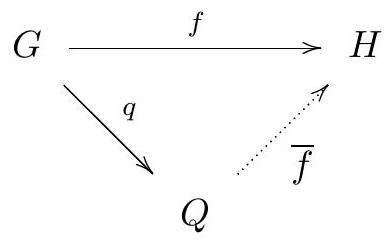
\includegraphics[max width=\textwidth, center]{2025_06_13_6ba93caed1e95a95104eg-037}\\
kommutiert, und $\bar{f}$ ist der einzige Homomorphismus $Q \rightarrow H$, für den das gilt.\\
Bevor wir einen Quotienten konstruieren, zeigen wir seine Eindeutigkeit! Dies illustriert, wie gut man mit den Eigenschaften umgehen kann, ohne zu wissen, ob es das Ding überhaupt gibt oder wie es konstruiert ist.

Proposition 5.10. Seien $G$ eine Gruppe und $N \subseteq G$ ein Normalteiler. Ein Quotient für $N \subseteq G$ ist eindeutig bis auf eindeutigen Isomorphismus.

Das bedeutet genauer: sind $q: G \rightarrow Q$ und $p: G \rightarrow P$ Quotienten für $N \subseteq G$, dann gibt es eindeutige Isomorphismen

$$
\varphi: Q \rightarrow P, \quad \psi: P \rightarrow Q,
$$

so daß $p=\varphi \circ q$ und $q=\psi \circ p$. Es sind $\varphi$ und $\psi$ zueinander invers.\\
Beweis. Weil $N \subseteq \operatorname{ker}(p)$ und $q: G \rightarrow Q$ ein Quotient ist (bzw. weil $N \subseteq \operatorname{ker}(q)$ und $p: G \rightarrow P$ ein Quotient ist), schließen wir aus der universellen Eigenschaft auf eindeutige Homomorphismen $\varphi$ (bzw. $\psi$ ) wie im kommutativen Diagramm:\\
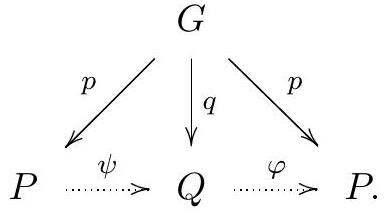
\includegraphics[max width=\textwidth, center]{2025_06_13_6ba93caed1e95a95104eg-038}

Damit erfüllt $\varphi \circ \psi$ die von der universellen Eigenschaft gestellte Anforderung im Fall $f:=p$, genauso wie $\operatorname{id}_{P}: P \rightarrow P$. Die geforderte Eindeutigkeit erzwingt $\varphi \circ \psi=\operatorname{id}_{P}$. Aus Symmetrie folgt $\psi \circ \varphi=\operatorname{id}_{Q}$. Dies zeigt, daß $\varphi$ und $\psi$ sogar zueinander inverse Isomorphismen sind und weiter die Eindeutigkeit des Quotienten.

Nachdem die Eindeutigkeit geklärt ist, gilt es, einen Quotienten zu konstruieren.\\
Satz 5.11 (Existenz des Quotienten nach einem Normalteiler). Seien G eine Gruppe und N $\subseteq G$ ein Normalteiler. Dann ist die Faktorgruppe $G / N$ zusammen mit dem Gruppenhomomorphismus

$$
p: G \rightarrow G / N, \quad p(g)=g N
$$

ein Quotient für $N \subseteq G$.\\
Beweis. Es gilt $N=\operatorname{ker}(p)$. Es gilt somit (i) aus Definition 5.9.\\
Sei nun $f: G \rightarrow H$ ein Gruppenhomomorphismus mit $N \subseteq \operatorname{ker}(f)$. Dann ist $f$ konstant auf Nebenklassen von $N$, denn

$$
f(g N)=f(g) f(N)=f(g) .
$$

Damit ist die Abbildung

$$
\begin{aligned}
\bar{f}: G / N & \rightarrow H \\
g N & \mapsto f(g)
\end{aligned}
$$

wohldefiniert. Außerdem ist $\bar{f}$ ein Gruppenhomomorphismus:

$$
\bar{f}(g N \cdot h N)=\bar{f}(g h N)=f(g h)=f(g) \cdot f(h)=\bar{f}(g N) \cdot \bar{f}(h N) .
$$

Es gilt offensichtlich $f=\bar{f} \circ p$

$$
f(g)=\bar{f}(g N)=\bar{f}(p(g)) .
$$

Jeder Homomorphismus $\varphi: G / N \rightarrow H$ mit $f=\varphi \circ p$ stimmt mit $\bar{f}$ überein, weil $p$ surjektiv ist:

$$
\varphi(g N)=\varphi(p(g))=f(g)=\bar{f}(p(g))=\bar{f}(g N) .
$$

Dies zeigt die Eindeutigkeit der geforderten Faktorisierung in (ii) aus Definition 5.9.

Bemerkung 5.12. Aus dem Beweis von Satz 5.11 folgt, daß Faktorgruppen $G / N$ zusammen mit der natürlichen Abbildung $G \rightarrow G / N$ Quotienten sind. Wegen der Eindeutigkeit des Quotienten, Proposition 5.10, sind Quotientenabbildungen für Normalteiler $N \subseteq G$ immer surjektiv, und der Kern ist gleich $N$. Das folgt nicht aus der definierenden universellen Eigenschaft des Quotienten, sondern aus der Konstruktion mittels Faktorgruppe und der Eindeutigkeit.

Beispiel 5.13 (Quotienten von $\mathbb{Z}$ ). Die Gruppe $\mathbb{Z}$ ist abelsch und daher jede Untergruppe auch Normalteiler. Für $N=\{0\}$ ist $\mathbb{Z} / N=\mathbb{Z}$ und die Quotientenabbildung die Identität. Sei $n>0$ eine natürliche Zahl. Wir betrachten nun den Normalteiler $N=n \mathbb{Z}$. Dann ist

$$
\mathbb{Z} / n \mathbb{Z}
$$

die Gruppe bestehend aus den Nebenklassen

$$
a+n \mathbb{Z} \in \mathbb{Z} / n \mathbb{Z} .
$$

Die Addition in $\mathbb{Z} / n \mathbb{Z}$ wird mittels Addition in $\mathbb{Z}$ von Vertretern definiert. Die Faktorgruppe $\mathbb{Z} / n \mathbb{Z}$ ist also nichts anderes als die Gruppe der Restklassen modulo $n$ mit derselben Notation!\\
5.3. Die Isomorphiesätze. Wir kommen nun zu klassischen Isomorphiesätzen. Der erste, der Homomorphiesatz, beweist die anderen Isomorphiesätze als Spezialfall, und ist doch selbst im Grunde ein Spezialfall der Existenz und Eindeutigkeit von Quotienten nach Normalteilern.

Beispiel 5.14. Sei $n \geq 2$. Die alternierende Gruppe $A_{n}$ ist der Kern des Signumhomomorphismus und daher ein Normalteiler von $S_{n}$. Die Nebenklassen sind die Mengen konstanten Signums, daher parametrisiert man $S_{n} / A_{n}$ am besten mittels des Signums als $\{ \pm 1\}$. Es fällt nicht schwer, dies als Isomorphismus

$$
S_{n} / A_{n} \simeq\{ \pm 1\}
$$

zu erkennen. Dies ist ein Beispiel für den folgenden Satz, hier angewandt auf sign : $S_{n} \rightarrow\{ \pm 1\}$.\\
Satz 5.15 (Homomorphiesatz). Sei $f: G \rightarrow H$ ein Gruppenhomomorphismus. Dann gibt es einen Isomorphismus

$$
\varphi: G / \operatorname{ker}(f) \xrightarrow{\sim} \operatorname{im}(f), \quad g \operatorname{ker}(f) \mapsto f(g) .
$$

Beweis. Der Kern $N=\operatorname{ker}(f)$ ist ein Normalteiler und $p: G \rightarrow G / N$ ein Quotient. Daher faktorisiert $f$ eindeutig über einen Gruppenhomomorphismus

$$
\tilde{\varphi}: G / N \rightarrow H
$$

mit $f=\tilde{\varphi} \circ p$. Weil $p$ surjektiv ist, nimmt $\tilde{\varphi}$ nur Werte

$$
\tilde{\varphi}(g N)=f(g) \in \operatorname{im}(f)
$$

an. Man kann daher $\tilde{\varphi}$ eindeutig als Komposition eines Gruppenhomomorphismus

$$
\varphi: G / N \rightarrow \operatorname{im}(f)
$$

und der Inklusion $i: \operatorname{im}(f) \hookrightarrow H$ schreiben. Es ergibt sich das folgende kommutative Diagramm\\
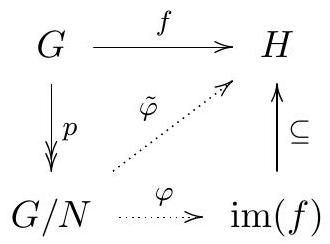
\includegraphics[max width=\textwidth, center]{2025_06_13_6ba93caed1e95a95104eg-039}

Zu zeigen bleibt, daß $\varphi$ ein Isomorphismus ist.\\
Wir bestimmen den Kern von $\varphi$. Sei $g N \in G / N$ ein Element im Kern von $\varphi$. Dann ist

$$
f(g)=\varphi(g N)=1
$$

also $g \in N$. Damit ist $g N=N$ und $\operatorname{ker}(\varphi)=1$. Somit ist $\varphi$ injektiv nach Proposition 2.14.

Die Abbildung $\varphi$ ist surjektiv, denn für jedes $h \in \operatorname{im}(f)$ gibt es $g \in G$ mit $f(g)=h$ und

$$
\varphi(g N)=f(g)=h
$$

Damit ist $\varphi$ sogar bijektiv und ein Isomorphismus.\\
Korollar 5.16. Sei $f: G \rightarrow H$ ein Gruppenhomomorphismus. Dann hat $\operatorname{ker}(f)$ endlichen Index genau dann, wenn $\operatorname{im}(f)$ endliche Ordnung hat. Es gilt dann:

$$
(G: \operatorname{ker}(f))=|\operatorname{im}(f)| .
$$

Beweis. Das folgt aus dem Homomorphiesatz, Satz 5.15, oder bereits aus Proposition 4.10.\\
Korollar 5.17. Sei $f: G \rightarrow H$ ein Gruppenhomomorphismus. Wenn $G$ eine endliche Gruppe ist, dann gilt

$$
|G|=|\operatorname{ker}(f)| \cdot|\operatorname{im}(f)| .
$$

Beweis. Das folgt sofort aus Korollar 5.16 und dem Satz von Lagrange, Satz 4.12,

$$
|G|=|\operatorname{ker}(f)| \cdot(G: \operatorname{ker}(f))=|\operatorname{ker}(f)| \cdot|\operatorname{im}(f)| .
$$

Beispiel 5.18. Sei $G$ eine Gruppe. In Satz 3.18 haben wir bereits eine Version des Homomorphiesatzes bewiesen, und zwar für die Exponentialabbildung $\varphi(a)=g^{a}$ zu einem Element $g \in G$. Der Gruppenhomomorphismus $\varphi: \mathbb{Z} \rightarrow G$ hat $\operatorname{Kern} \operatorname{ker}(\varphi)=n \mathbb{Z}$ für

$$
n= \begin{cases}\operatorname{ord}(g) & \text { wenn } g \text { endliche Ordnung hat } \\ 0 & \text { falls ord }(g)=\infty\end{cases}
$$

und induziert einen Gruppenisomorphismus

$$
\mathbb{Z} / n \mathbb{Z} \xrightarrow{\sim} \operatorname{im}(\varphi)=\langle g\rangle .
$$

Das ist nichts anderes als der Homomorphiesatz, Satz 5.15, angewandt auf $\varphi$.\\
Satz 5.19 (Erster Isomorphiesatz). Seien $G$ eine Gruppe, $H \subseteq G$ eine Untergruppe und $N \subseteq G$ ein Normalteiler. Dann ist

$$
\begin{aligned}
H /(H \cap N) & \xrightarrow{\sim} H N / N \\
h(H \cap N) & \mapsto h N
\end{aligned}
$$

ein Gruppenisomorphismus. Insbesondere gilt:\\
(1) Das Produkt in $G$ von Mengen

$$
H N=\{h n ; h \in H, n \in N\} \subseteq G
$$

ist eine Untergruppe in $G$, und\\
(2) $N \subseteq H N$ ist ein Normalteiler.\\
(3) $N \cap H$ ist ein Normalteiler in $H$.

Beweis. (1) Sei $i: H \hookrightarrow G$ die Inklusion und $p: G \rightarrow G / N$ die Quotientenabbildung. Die Abbildung

$$
f=p \circ i: H \rightarrow G \rightarrow G / N
$$

ist ein Gruppenhomomorphismus und

$$
H N=p^{-1}(f(H))
$$

ist eine Untergruppe als Urbild einer Untergruppe.\\
(2) Es gilt $N \subseteq H N$ und als Normalteiler in $G$ ist $N$ Normalteiler in jeder Untergruppe von $G$, in der $N$ enthalten ist.\\
(3) Der Kern von $f$ ist $f^{-1}(1)=i^{-1}(N)=H \cap N$ und als Kern ist $H \cap N$ ein Normalteiler von $H$.

Nun beweisen wir die Isomorphieaussage. Per Konstruktion ist $H N / N \subseteq G / N$ eine Untergruppe. Genauer ist $H N / N$ das Bild von $f: H \rightarrow G / N$ wie oben. Der Homomorphiesatz, Satz 5.15, angewandt auf $f$ liefert den gesuchten Isomorphismus

$$
\varphi: H /(H \cap N) \xrightarrow{\sim} H N / N
$$

denn für alle $h \in H$ gilt $\varphi(h(H \cap N))=f(h)=h N$ nach Konstruktion von $\varphi$ wie in Satz 5.15.\\
Beispiel 5.20. (1) Sei $G=\mathbb{Z}, H=5 \mathbb{Z}$ und $N=3 \mathbb{Z}$. Dann ist $H \cap N=15 \mathbb{Z}$ und wegen $1=2 \cdot 3-5$ gilt $H N=\mathbb{Z}$. Nach dem ersten Isomorphiesatz gilt

$$
5 \mathbb{Z} / 15 \mathbb{Z} \simeq \mathbb{Z} / 3 \mathbb{Z}
$$

(2) Sei $K$ ein Körper und $n \in \mathbb{N}$. Sei $\mathbf{1} \in \operatorname{GL}_{n}(K)$ die Einheitsmatrix. Die Gruppe $D \subseteq$ $\mathrm{GL}_{n}(K)$ der Diagonalmatrizen mit konstantem Eintrag auf der Diagonale aus $K^{\times}$ist isomorph zu $K^{\times}$vermöge

$$
\begin{aligned}
& K^{\times} \rightarrow D \\
& \lambda \mapsto \lambda \mathbf{1}=\left(\begin{array}{cccc}
\lambda & 0 & \ldots & 0 \\
0 & \ddots & \ddots & \vdots \\
\vdots & \ddots & \ddots & 0 \\
0 & \ldots & 0 & \lambda
\end{array}\right)
\end{aligned}
$$

Ferner ist $D$ ein Normalteiler in $\operatorname{GL}_{n}(K)$, denn für $\lambda \in K^{\times}$und $A \in \operatorname{GL}_{n}(K)$ gilt

$$
A(\lambda \mathbf{1}) A^{-1}=\lambda\left(A \mathbf{1} A^{-1}\right)=\lambda\left(A A^{-1}\right)=\lambda \mathbf{1}
$$

Die Faktorgruppe ist

$$
\operatorname{PGL}_{n}(K)=\operatorname{GL}_{n}(K) / D
$$

genannt die projektiv lineare Gruppe.\\
(3) Wir betrachten nun $H=\operatorname{SL}_{n}(K)$ als Untergruppe von $\operatorname{GL}_{n}(K)$. Dann ist

$$
\mu_{n}(K):=\left\{\lambda \in K^{\times} ; \lambda^{n}=1\right\}
$$

über die Einschränkung des Isomorphismus $K^{\times} \simeq D$ selbst isomorph zu

$$
\mu_{n}(K) \simeq D_{n}:=\operatorname{SL}_{n}(K) \cap D
$$

Der erste Isomorphiesatz liefert dann den Isomorphismus

$$
\operatorname{SL}_{n}(K) / D_{n} \xrightarrow{\sim} \operatorname{SL}_{n}(K) D / D
$$

auf die Untergruppe

$$
\operatorname{PSL}_{n}(K):=\operatorname{SL}_{n}(K) D / D \subseteq \operatorname{GL}_{n}(K) / D=\operatorname{PGL}_{n}(K) .
$$

Satz 5.21 (Zweiter Isomorphiesatz). Sei $G$ eine Gruppe und $N$ und $K$ seien Normalteiler in $G$ mit $N \subseteq K \subseteq G$. Dann ist

$$
\begin{aligned}
(G / N) /(K / N) & \xrightarrow{\sim} G / K \\
g N(K / N) & \mapsto g K
\end{aligned}
$$

ein Gruppenisomorphismus. Insbesondere ist $K / N$ ein Normalteiler in $G / N$.\\
Beweis. Die Quotientenabbildung $p: G \rightarrow G / K$ hat Kern $K$, daher gilt $p(N)=1$. Die universelle Eigenschaft aus Satz 5.11 des Quotienten $q: G \rightarrow G / N$ liefert einen eindeutigen Gruppenhomomorphismus

$$
f: G / N \rightarrow G / K
$$

mit

$$
f(g N)=f(q(g))=p(g)=g K
$$

Die Abbildung $f$ ist offensichtlich surjektiv und $\operatorname{ker}(f)=K / N$, denn $g K=K$ bedeutet $g \in K$. Der Homomorphiesatz, Satz 5.15, angewandt auf $f$ liefert den gesuchten Isomorphismus

$$
\varphi:(G / N) /(K / N) \xrightarrow{\sim} G / K
$$

und $\varphi(g N(K / N))=f(g N)=g K$ wie behauptet.\\
Beispiel 5.22. Seien $n, m \in \mathbb{N}$ natürliche Zahlen. Dann ist $m n \mathbb{Z} \subseteq m \mathbb{Z} \subseteq \mathbb{Z}$. Nach dem zweiten Isomorphiesatz gilt dann

$$
(\mathbb{Z} / n m \mathbb{Z}) /(m \mathbb{Z} / n m \mathbb{Z}) \simeq \mathbb{Z} / m \mathbb{Z} .
$$

5.4. Kommutatoren und abelsche Quotienten. Kommutatoren messen die Abweichung von Kommutativität.

Definition 5.23. Der Kommutator zweier Gruppenelemente $g, h \in G$ ist das Element

$$
[g, h]=g h g^{-1} h^{-1} \in G
$$

Notation 5.24. Unter Gruppentheoretikern ist auch die Notation

$$
(g, h)=g^{-1} h^{-1} g h=g^{-1} g^{h}
$$

geläufig. Das ist im Sinne dieses Skripts nichts weiter als der Kommutator der inversen Elemente.\\
Lemma 5.25. Seien $g, h \in G$ Gruppenelemente. Dann kommutieren $g$ und $h$ genau dann, wenn gilt:

$$
[g, h]=1
$$

Beweis. Es gilt $g h=h g$ genau dann, wenn $[g, h]=g h g^{-1} h^{-1}=h g\left(g^{-1} h^{-1}\right)=1$ gilt.\\
Lemma 5.26. Sei $f: G \rightarrow H$ ein Gruppenhomomorphismus. Für alle $x, y \in G$ gilt

$$
f([x, y])=[f(x), f(y)]
$$

Beweis. Das ist trivial.\\
Definition 5.27. Die Kommutator(unter)gruppe einer Gruppe $G$ ist die Untergruppe

$$
[G, G]=\langle[g, h] ; g, h \in G\rangle
$$

welche von allen Kommutatoren in $G$ erzeugt wird.\\
Notation 5.28. Als Notation für die Kommutatorgruppe zu $G$ findet man auch $G^{\prime}=[G, G]$.\\
Lemma 5.29. Sei $f: G \rightarrow H$ ein Gruppenhomomorphismus. Dann gilt

$$
f([G, G]) \subseteq[H, H]
$$

Beweis. Das folgt aus Lemma 5.26 und Proposition 2.26.\\
Proposition 5.30 (Kommutatorfaktorgruppe). Sei G eine Gruppe. Dann ist die Kommutatorgruppe $[G, G]$ ein Normalteiler in $G$, und die Faktorgruppe $G /[G, G]$ ist abelsch.

Wir nennen die Gruppe $G /[G, G]$ die Kommutatorfaktorgruppe von $G$.\\
Beweis. Seien $g, x, y \in G$ beliebig und $a=g x g^{-1}$ und $b=g y g^{-1}$. Dann ist

$$
g[x, y] g^{-1}=\varphi_{g}([x, y])=\varphi_{g}\left(x y x^{-1} y^{-1}\right)=\varphi_{g}(x) \varphi_{g}(y) \varphi_{g}(x)^{-1} \varphi_{g}(y)^{-1}=[a, b]
$$

Daher gilt

$$
g[G, G] g^{-1}=\varphi_{g}(\langle[x, y] ; x, y \in G\rangle)=\left\langle\varphi_{g}([x, y]) ; x, y \in G\right\rangle \subseteq\langle[a, b] ; a, b \in G\rangle=[G, G]
$$

Nach Proposition 14.31 ist damit $[G, G]$ ein Normalteiler in $G$.\\
Seien $\bar{a}, \bar{b} \in G /[G, G]$ beliebige Elemente und $a, b \in G$ mit $p(a)=\bar{a}$ und $p(b)=\bar{b}$. Dann:

$$
[\bar{a}, \bar{b}]=p(a) p(b) p(a)^{-1} p(b)^{-1}=p\left(a b a^{-1} b^{-1}\right)=p([a, b])=1
$$

Also ist $G /[G, G]$ kommutativ.

Definition 5.31. Die Abelisierung einer Gruppe $G$ ist eine abelsche Gruppe $G^{\text {ab }}$ zusammen mit einem Homomorphismus $p: G \rightarrow G^{\text {ab }}$, so daß es für alle Homomorphismen $f: G \rightarrow H$ mit Ziel in einer abelschen Gruppe $H$ einen eindeutigen Homomorphismus

$$
\varphi: G^{\mathrm{ab}} \rightarrow H
$$

gibt mit $f=\varphi \circ p$.\\
Die Eindeutigkeit der Abelisierung folgt dem gewohnten Muster bei universellen Eigenschaften. Wir beschränken uns deshalb darauf zu zeigen, daß die Kommutatorfaktorgruppe eine (die) Abelisierung ist.

Satz 5.32 (Abelisierung). Sei G eine Gruppe. Dann hat die Quotientenabbildung

$$
p: G \rightarrow G /[G, G]
$$

die universelle Eigenschaft der Abelisierung.\\
Beweis. Die Gruppe $G /[G, G]$ ist abelsch nach Proposition 5.30.\\
Sei $f: G \rightarrow H$ ein beliebiger Homomorphismus mit einer abelschen Gruppe $H$ als Ziel. Dann gilt für beliebige Elemente $x, y \in G$ :

$$
f([x, y])=[f(x), f(y)]=1
$$

also gilt $[G, G] \subseteq \operatorname{ker}(f)$. Die Existenz und Eindeutigkeit der Faktorisierung folgt nun aus der universellen Eigenschaft des Quotienten nach Satz 5.11 zusammen damit, daß $p: G \rightarrow G /[G, G]$ eine Quotientenabbildung ist.

\section*{ÜBUNGSAUFGABEN ZU §5}
Übungsaufgabe 5.1. (Die universelle Eigenschaft des Produkts) Sei $I$ eine Menge und $G_{i}$ eine Gruppe für jedes $i \in I$. Ein Produkt der Gruppen $G_{i}$ besteht aus einer Gruppe $P$ zusammen mit Homomorphismen für alle $i \in I$

$$
p_{i}: P \rightarrow G_{i},
$$

so daß die universelle Eigenschaft für Produkte gilt: für jede Gruppe $\Gamma$ und Gruppenhomomorphismen $f_{i}: \Gamma \rightarrow G_{i}$ für alle $i \in I$ existiert ein eindeutiger Gruppenhomomorphismus

$$
f: \Gamma \rightarrow P
$$

mit $p_{i} \circ f=f_{i}$.\\
Zeigen Sie, daß $\prod_{i \in I} G_{i}$ zusammen mit den Projektionen $\operatorname{pr}_{j}: \prod_{i \in I} G_{i} \rightarrow G_{j}$ ein Produkt der Gruppen $G_{i}$ ist. Zeigen Sie weiter, daß jedes Produkt $P$ der $G_{i}$ auf eindeutige Weise zu $\prod_{i \in I} G_{i}$ isomorph ist, d.h., es gibt einen eindeutigen Isomorphismus

$$
\varphi: P \xrightarrow{\sim} \prod_{i \in I} G_{i}
$$

mit $p_{i}=\operatorname{pr}_{i} \circ \varphi$.\\
Übungsaufgabe 5.2. Sei $\mathbb{F}$ ein endlicher Körper mit $q$ Elementen. Berechnen Sie die Ordnung der Gruppe $\mathrm{PGL}_{n}(\mathbb{F})$.

Übungsaufgabe 5.3. Zeigen Sie, daß die Operation von $\operatorname{GL}_{n+1}(K)$ auf $\mathbb{P}^{n}(K)$ aus Aufgabe 13.5 eine Operation von $\mathrm{PGL}_{n+1}(K)$ auf $\mathbb{P}^{n}(K)$ induziert.

Übungsaufgabe 5.4. Seien $H$ und $N$ Untergruppen von $G$. Dann ist das naive mengentheoretische Produkt

$$
H N=\{h k ; h \in H, k \in N\}
$$

in der Regel keine Untergruppe von $G$ mehr. Geben Sie ein Beispiel.\\
Zeigen Sie, daß $H N$ eine Untergruppe von $G$ ist, sofern $N$ ein Normalteiler von $G$ ist.

Übungsaufgabe 5.5. Bestimmen Sie die Kommutatorfaktorgruppe von $S_{n}$.\\
Übungsaufgabe 5.6. Sei $G \rightarrow H$ ein surjektiver Gruppenhomomorphismus, und sei $U \subseteq G$ eine Untergruppe mit $\operatorname{ker}(f) \subseteq U$. Dann gilt

$$
(G: U)=(H: f(U))
$$

Übungsaufgabe 5.7. Seien $f_{i}: G_{i} \rightarrow H$ für $i=1,2$ surjektive Gruppenhomomorphismen und $G_{1} \times{ }_{H} G_{2}$ das entsprechende Faserprodukt. Zeigen Sie

$$
\left(G_{1} \times G_{2}: G_{1} \times{ }_{H} G_{2}\right)=|H| .
$$

Tipp: benutzen sie den Gruppenhomomorphismus ( $f_{1}, f_{2}$ ): $G_{1} \times G_{2} \rightarrow H \times H$, Aufgabe 5.6, sowie

$$
(H \times H: \Delta(H))=|H|,
$$

wobei $\Delta$ die Diagonale $\Delta: H \rightarrow H \times H, \Delta(h)=(h, h)$ ist.\\
Übungsaufgabe 5.8. Mit der Notation aus Beispiel 4.23 gilt

$$
\left(S_{8} \times S_{12}: \rho\left(\mathscr{R}_{3}\right)\right)=2
$$

Teil 2. Ringe

\section*{Ringe}
6.1. Beispiele, elementare Regeln und Homomorphismen. Ringe sind Strukturen mit Addition und Multiplikation.

Definition 6.1. (1) Ein Ring (mit Eins) ist eine Menge $R$ zusammen mit Verknüpfungen Addition

$$
+: R \times R \rightarrow R
$$

und Multiplikation

$$
\cdot: R \times R \rightarrow R
$$

mit den folgenden Eigenschaften.\\
(i) $(R,+)$ ist eine abelsche Gruppe.\\
(ii) Die Multiplikation ist assoziativ: für alle $a, b, c \in R$ gilt

$$
a \cdot(b \cdot c)=(a \cdot b) \cdot c
$$

(iii) Addition und Multiplikation sind distributiv: für alle $a, b, r \in R$ gilt

$$
\begin{aligned}
& r \cdot(a+b)=(r \cdot a)+(r \cdot b) \\
& (a+b) \cdot r=(a \cdot r)+(b \cdot r)
\end{aligned}
$$

(iv) Es gibt ein neutrales Element $1 \in R$ für die Multiplikation: für alle $a \in R$ gilt

$$
1 \cdot a=a=a \cdot 1
$$

(2) Ein kommutativer Ring ist ein Ring, so daß für alle $a, b \in R$ gilt

$$
a \cdot b=b \cdot a
$$

Bemerkung 6.2. Der Name hat nichts mit der Geometrie eines ringförmigen Objekts zu tun. Es geht um den Zusammenschluß von Elementen zu einer Gesamtstruktur, ähnlich einer juristischen Person (Weißer Ring, etc.). Dabei steht (juristisch) Ring in Abgrenzung zu (juristisch) Körper(schaft) als eine Organisationsstruktur mit einer Regel weniger: es wird nicht gefordert, daß es für Elemente $a \neq 0$ ein Inverses $a^{-1}$ bezüglich der Multiplikation gibt.

Notation 6.3. (1) Die Multiplikation kürzen wir ab durch

$$
a b:=a \cdot b .
$$

Außerdem gilt 'Punkt vor Strich'. Diese Festlegung spart Klammern.\\
(2) Das neutrale Element der Addition wird mit 0 bezeichnet, das additive Inverse zu $a \in R$ hat die Notation

\section*{$-a$}
also $a+(-a)=(-a)+a=0$. Statt $a+(-b)$ schreiben wir wie gewöhnlich $a-b$.\\
(3) Zu $a \in R$ und $n \in \mathbb{N}_{0}$ definieren wir rekursiv $a^{0}=1$ und

$$
a^{n}:=a \cdot a^{n-1}
$$

Damit ist $a^{n}=a \cdot \ldots \cdot a$ mit $n$-Faktoren $a$. Es gelten die erwarteten Potenzgesetze

$$
\begin{aligned}
a^{n} a^{m} & =a^{n+m}, \\
\left(a^{n}\right)^{m} & =a^{n m}, \\
(a b)^{n} & =a^{n} b^{n} . \quad(\text { nur wenn } a b=b a)
\end{aligned}
$$

Beispiel 6.4. (1) Jeder Körper ist ein Ring: $\mathbb{Q}, \mathbb{R}, \mathbb{F}_{p}, \mathbb{C}, \ldots$\\
(2) Die ganzen Zahlen $\mathbb{Z}$ bilden einen Ring mit der üblichen Addition und Multiplikation.\\
(3) Sei $X$ eine Menge und $R$ ein Ring. Dann ist die Menge

$$
\operatorname{Abb}(X, R):=\{f ; f: X \rightarrow R \text { Abbildung }\}
$$

der Abbildungen von $X$ nach $R$ ein Ring, der Ring der Funktionen von $X$ nach $R$, und zwar mit punktweiser Addition und Multiplikation: für $f_{1}, f_{2} \in \operatorname{Abb}(X, R)$ und $x \in X$ gilt

$$
\begin{aligned}
\left(f_{1}+f_{2}\right)(x) & =f_{1}(x)+f_{2}(x) \\
\left(f_{1} \cdot f_{2}\right)(x) & =f_{1}(x) \cdot f_{2}(x)
\end{aligned}
$$

Die Ringaxiome sind erfüllt, weil sie in $R$ erfüllt sind. Man überlege sich dies!\\
(4) Sei $K$ ein Körper und $n \in \mathbb{N}$. Dann ist $\mathrm{M}_{n}(K)$, der Matrizenring (über $K$ ), ein Ring mit der üblichen Matrizenmultiplikation und Matrizenaddition.\\
(5) Sei $V$ ein $K$-Vektorraum. Dann ist $\operatorname{End}_{K}(V)$ ein Ring bezüglich Addition und Komposition von linearen Abbildungen.\\
(6) Sei $R$ ein Ring und $n \in \mathbb{N}$. Matrizen mit Einträgen in $R$ lassen sich genauso addieren und multiplizieren wie Matrizen mit Einträgen in einem Körper. Mit der üblichen Matrizenmultiplikation und Matrizenaddition ist $\mathrm{M}_{n}(R)$, der Matrizenring (über $R$ ), ein Ring.\\
(7) Der Nullring ist der einzige Ring mit genau einem Element. Addition und Multiplikation ergeben sich von selbst.\\
(8) Sei $A$ eine Menge und zu $\alpha \in A$ ein Ring $R_{\alpha}$ gegeben. Dann definiert komponentenweise Addition und Multiplikation eine Ringstruktur auf dem Produkt

$$
R:=\prod_{\alpha \in A} R_{\alpha}
$$

Die Eins des Produkts $R$ ist das Tupel $\left(1_{R_{\alpha}}\right)_{\text {ain } A}$, das an jeder Stelle aus der jeweiligen Eins besteht.

Das Produkt von Ringen ist eine Konstruktion analog zum Produkt von Gruppen, vgl. Definition 1.9, oder zum Produkt von Mengen.\\
Beispiel 6.5. Sei $G$ eine Gruppe und $K$ ein Körper. Der Gruppenring mit Koeffizienten aus $K$ ist der Ring

$$
K[G]=\bigoplus_{g \in G} K \cdot g
$$

also als $K$-Vektorraum einfach die direkte Summe von 1-dimensionalen Vektorräumen mit Basis $g$ für jedes Gruppenelement $g \in G$. Elemente von $K[G]$ sind daher endliche Summen

$$
a=\sum_{g \in G} a(g) g
$$

mit $a(g) \in K$ und alle bis auf endlich viele $a(g)=0$. Dies kann man auch als Funktionen

$$
a: G \rightarrow K
$$

auffassen mit einem Wert $\neq 0$ an nur endlich vielen Stellen $g \in G$. Die Basisvektoren $g \in K \cdot g$ liefern Elemente $g \in K[G]$.

Die Addition von $K[G]$ ist die Addition als Vektorraum. Die Multiplikation wird definiert für $a, b \in K[G]$ durch (Faltung)

$$
a \cdot b(g)=\sum_{x, y \in G, x y=g} a(x) b(y)
$$

Dies ist wohldefiniert, weil nur endlich viele $x$ und endlich viele $y$ zu $a(x) \neq 0 \neq b(y)$ führen: die Summe ist eine endliche Summe. Diese Multiplikation setzt die Gruppenverknüpfung auf den Elementen $g \in K[G]$ für $g \in G$ linear fort: für alle $g, h \in G$ gilt

$$
g \cdot h=g h
$$

Wir überlassen den Nachweis der Ringaxiome als Übungsaufgabe.

Bemerkung 6.6. Manchmal versteht man unter einem Ring einen Ring ohne Eins, also eine Menge $R$ mit + und , so daß (i)-(iii) der obigen Definition gelten. Dies tun wir hier nicht. Manchmal wird für Ringe mit Eins noch verlangt, daß $0 \neq 1$ gilt. Das tun wir hier auch nicht, um den Nullring nicht auszuschließen.

Die Eins in einem Ring ist eindeutig. Das geht wie beim neutralen Element einer Gruppe. Sind 1 und $1^{\prime}$ Einsen, dann gilt

$$
1=1 \cdot 1^{\prime}=1^{\prime}
$$

Es gelten die üblichen Rechenregeln für - , insbesondere das Distributivgesetz mit - statt + .\\
Lemma 6.7. Sei $R$ ein Ring. Dann gilt für alle $a, b, c \in R$\\
(1) $0 \cdot a=a \cdot 0=0$,\\
(2) $(-a) b=a(-b)=-(a b)$,\\
(3) $a(b-c)=a b-a c$ und $(a-b) c=a c-b c$.\\
(4) $(-a)(-b)=a b$.\\
(5) $-a=(-1) a=a(-1)$.

Beweis. (1) Aus $0 a=(0+0) a=0 a+0 a$ folgt durch Addition mit $-(0 a)$ schon $0=0 a$. Die Gleichung $a 0=0$ folgt analog.\\
(2) Wegen $a b+(-a) b=(a+(-a)) b=0 b=0$ folgt $(-a) b=-(a b)$. Die andere Gleichung folgt analog.\\
(3) Es gilt $a(b-c)=a(b+(-c))=a b+a(-c)=a b+(-a c)=a b-a c$. Die andere Gleichung folgt analog.\\
(4) Wir verwenden zweimal (2) und rechnen: $(-a)(-b)=-(a)(-b)=-(-(a b))=a b$.\\
(5) Aus (2) folgt $(-1) a=-(1 a)=-a$. Die andere Gleichung folgt analog.

Lemma 6.8. Sei $0=1$ in einem Ring $R$, dann ist $R$ der Nullring.\\
Beweis. Sei $a \in R$ ein beliebiges Element. Dann gilt

$$
a=a \cdot 1=a \cdot 0=0
$$

und $R$ enthält nur ein einziges Element.\\
Bemerkung 6.9. Jeder Ring ist ein Ring von geeigneten Funktionen auf einer Menge. Das Beispiel $\operatorname{Abb}(X, R)$ ist also gut für die Intuition, aber trotzdem noch eine grobe Approximation, denn man muß akzeptieren, daß der Wertebereich der Funktionen von $x \in X$ abhängt. So ist beispielsweise $\mathbb{Z}$ der Ring der algebraischen Funktionen auf $\operatorname{Spec}(\mathbb{Z})$, einer Menge die im Wesentlichen aus den Primzahlen besteht. Der Wert von $n \in \mathbb{Z}$ an der Primzahl $p$ ist die Restklasse $n \bmod p$ in $\mathbb{F}_{p}=\mathbb{Z} / p \mathbb{Z}$. Man kann zumindest sehen, daß diese Funktionswerte die ganzen Zahlen als Funktionen eindeutig festlegen. Denn falls für $n, m \in \mathbb{Z}$ und alle Primzahlen $p$ gilt $n \equiv m$ $\bmod p$, so wählen wir einfach eine Primzahl $p$, die größer als $2 \max \{|n|,|m|\}$ ist, und finden wegen

$$
-p<n-m<p
$$

und $p \mid n-m$, daß $n=m$ sein muß. Entscheidend geht hier ein, daß es unendlich viele Primzahlen in $\mathbb{Z}$ gibt und damit die gewünschte Wahl von $p$ auch durchgeführt werden kann. Wenn Sie nicht wissen, wie man beweist, daß es unendlich viele Primzahlen gibt, dann holen Sie das schnellstmöglich nach. Speziell Euklids Beweis hierfür sollte jede/r Mathematikstudierende kennen.

Beispiel 6.10. Die Menge der geraden ganzen Zahlen $2 \mathbb{Z} \subseteq \mathbb{Z}$ ist für den allgemeineren Begriff des Rings, wo keine Eins gefordert wird, ein Unterring, und gleichzeitig ein Beispiel eines Rings ohne Eins.

Definition 6.11. Seien $n, k \in \mathbb{N}_{0}$. Der Binomialkoeffizient $\binom{n}{k}$ ist definiert als

$$
\left.\binom{n}{k}=\mid\{k \text {-elementige Teilmengen von }\{1, \ldots, n\}\} \right\rvert\,
$$

und damit eine ganze Zahl $\geq 0$. Für $0 \leq k \leq n$ gilt $\binom{n}{k}=\frac{n!}{k!(n-k)!}$ und sonst $\binom{n}{k}=0$.\\
Proposition 6.12 (Binomischer Lehrsatz). Seien $a, b \in R$ kommutierende Elemente: $a b=b a$. Dann gilt für alle $n \in \mathbb{N}_{0}$ :

$$
(a+b)^{n}=\sum_{k=0}^{n}\binom{n}{k} a^{k} b^{n-k}
$$

Beweis. Aus $a b=b a$ zeigt man zunächst per Induktion nach $k$, daß auch $b a^{k}=a^{k} b$ gilt.\\
Wir argumentieren nun per Induktion nach $n$. Der Anfang $n=0$ ist klar. Im Schritt von $n$ auf $n+1$ muß man bei

$$
(a+b)^{n+1}=(a+b) \cdot \sum_{k=0}^{n}\binom{n}{k} a^{k} b^{n-k}=\sum_{k=0}^{n+1}\left(\binom{n}{k}+\binom{n}{k-1}\right) a^{k} b^{n+1-k}
$$

das Element $b$ an $a^{k}$ „vorbeiziehen". Nun folgt die Formel durch Koeffizientenvergleich mittels der Rekursionsformel für Binomialkoeffizienten

$$
\binom{n+1}{k}=\binom{n}{k}+\binom{n}{k-1}
$$

Aus der $n+1$-elementigen Menge wählen wir einen Präsidenten. Die $k$-elementigen Teilmengen teilen sich auf in $\binom{n}{k}$-viele ohne und $\binom{n}{k-1}$-viele mit dem Präsidenten.

Wir wollen algebraische Strukturen stets zusammen mit den strukturerhaltenden Abbildungen untersuchen.

Definition 6.13. Ein Ringhomomorphismus (oder kürzer Homomorphismus) zwischen Ringen $R$ und $S$ ist eine Abbildung $f: R \rightarrow S$, so daß für alle $a, b \in R$ gilt:\\
(i) $\quad f(a+b)=f(a)+f(b)$,\\
(ii) $\quad f(a b)=f(a) f(b)$,\\
(iii) $\quad f(1)=1$.

Ein Ringisomorphismus ist ein bijektiver Ringhomomorphismus.\\
Bemerkung 6.14. (1) Für jeden Ringhomomorphismus $f: R \rightarrow S$ ist $f$ ein Gruppenhomomorphismus der zugrundeliegenden abelschen Gruppen. Inbesondere gilt für alle $a \in R$

$$
f(-a)=-f(a)
$$

(2) Ein Ringisomorphismus zu sein ist äquivalent dazu, daß es einen inversen Ringhomomorphismus gibt: das Inverse ist aufgrund der Bijektivität automatisch ein Ringhomomorphismus.

Beispiel 6.15. (1) Sei $R$ ein Ring und $\varphi: Y \rightarrow X$ eine Abbildung von Mengen. Der Pullback (oder Rückzug) ist der folgende Ringhomomorphismus:

$$
\varphi^{*}: \operatorname{Abb}(X, R) \rightarrow \operatorname{Abb}(Y, R), \quad \varphi^{*}(f)=f \circ \varphi,
$$

also $\left(\varphi^{*} f\right)(y)=f(\varphi(y))$ für alle $y \in Y$.\\
(2) Ist $i: Y \hookrightarrow X$ die Inklusion einer Teilmenge, dann ist der Pullback die Einschränkung

$$
i^{*}(f)=\left.f\right|_{Y}
$$

(3) Für eine einpunktige Menge $Y=\{y\}$ ist $\operatorname{Abb}(Y, R) \simeq R$. Die Abbildung $f \mapsto f(y)$ ist bijektiv und ein Ringisomorphismus.\\
(4) Ein Spezialfall des Pullback: zu $x \in X$ und der Inklusion $i: Y=\{x\} \hookrightarrow X$ ist

$$
\begin{aligned}
i^{*}: \operatorname{Abb}(X, R) & \rightarrow \operatorname{Abb}(\{x\}, R) \simeq R \\
f & \mapsto i^{*} f=f(x)
\end{aligned}
$$

Dies ist der Auswertungshomomorphismus im Punkt $x \in X$.\\
Beispiel 6.16. Die komplexe Konjugation $\mathbb{C} \rightarrow \mathbb{C}$ definiert durch

$$
z=x+i y \mapsto \bar{z}=x-i y
$$

ist ein Ringhomomorphismus, sogar ein Ringisomorphismus.\\
Beispiel 6.17. Sei $K$ ein Körper. Dann ist

$$
\begin{aligned}
K & \rightarrow \mathrm{M}_{2}(K) \\
a & \mapsto\left(\begin{array}{ll}
a & 0 \\
0 & 0
\end{array}\right)
\end{aligned}
$$

kein Ringhomomorphismus. Wohl aber ist mit der Einheitsmatrix $\mathbf{1}_{n} \in \mathrm{M}_{n}(K)$ die Abbildung

$$
\lambda \mapsto \lambda \mathbf{1}_{n}=\left(\begin{array}{ccc}
\lambda & 0 & 0 \\
0 & \ddots & 0 \\
0 & 0 & \lambda
\end{array}\right)
$$

ein Ringhomomorphismus $K \rightarrow \mathrm{M}_{n}(K)$.\\
Für einen $K$-Vektorraum $V$ ist $\lambda \mapsto \lambda \cdot \operatorname{id}_{V}$ ein Ringhomomorphismus. Dies ist die koordinatenfreie Version des Ringhomomorphismus $K \rightarrow \mathrm{M}_{n}(K)$.\\
6.2. Potenzreihenringe und Polynomringe. Wir kommen zu zwei wichtigen Beispielen für Ringe.

Definition 6.18. Sei $R$ ein Ring. Der Potenzreihenring mit Koeffizienten in $R$ und der (formalen) Variablen $X$ ist der Ring

$$
R[[X]]=\left\{\sum_{i=0}^{\infty} a_{i} X^{i} ; a_{i} \in R \text { für alle } i\right\}
$$

der formalen Potenzreihen mit der folgenden Addition und Multiplikation:

$$
\begin{aligned}
\left(\sum_{i=0}^{\infty} a_{i} X^{i}\right)+\left(\sum_{i=0}^{\infty} b_{i} X^{i}\right) & =\sum_{i=0}^{\infty}\left(a_{i}+b_{i}\right) X^{i} \\
\left(\sum_{i=0}^{\infty} a_{i} X^{i}\right) \cdot\left(\sum_{i=0}^{\infty} b_{i} X^{i}\right) & =\sum_{i=0}^{\infty}\left(\sum_{j+k=i} a_{j} b_{k}\right) X^{i}
\end{aligned}
$$

Die innere Summe geht hier über $0 \leq j \leq i$ mit $k=i-j$, aber in unserer Schreibweise ist es symmetrischer. Die Bedingung $j, k \geq 0$ nehmen wir stillschweigend dazu, denn $a_{j}$ und $b_{k}$ sind ja nur für $j, k \geq 0$ vorhanden. Insbesondere handelt es sich um eine endliche Summe, somit ist die Multiplikation in $R[[X]]$ wohldefiniert.

Die Ringaxiome verifiziert man leicht, etwa die Assoziativität:

$$
\begin{aligned}
\left(\sum_{i=0}^{\infty} a_{i} X^{i} \cdot \sum_{i=0}^{\infty} b_{i} X^{i}\right) \cdot \sum_{i=0}^{\infty} c_{i} X^{i} & =\sum_{i=0}^{\infty}\left(\sum_{j+k=i} a_{j} b_{k}\right) X^{i} \cdot \sum_{i=0}^{\infty} c_{i} X^{i} \\
& =\sum_{i=0}^{\infty}\left(\sum_{r+s=i}\left(\sum_{j+k=r} a_{j} b_{k}\right) c_{s}\right) X^{i} \\
& =\sum_{i=0}^{\infty}\left(\sum_{j+k+l=i} a_{j} b_{k} c_{l}\right) X^{i} \\
& =\sum_{i=0}^{\infty}\left(\sum_{r+s=i} a_{r}\left(\sum_{k+l=s} b_{k} c_{l}\right)\right) X^{i} \\
& =\sum_{i=0}^{\infty} a_{i} X^{i} \cdot \sum_{i=0}^{\infty}\left(\sum_{k+l=i} b_{k} c_{l}\right) X^{i}=\sum_{i=0}^{\infty} a_{i} X^{i} \cdot\left(\sum_{i=0}^{\infty} b_{i} X^{i} \cdot \sum_{i=0}^{\infty} c_{i} X^{i}\right)
\end{aligned}
$$

Notation 6.19. (1) Wir schreiben suggestiv

$$
\sum_{i=0}^{\infty} a_{i} X^{i}=a_{0}+a_{1} X+a_{2} X^{2}+\ldots .
$$

'Formale Variable' bedeutet, daß man nicht erwartet, hier etwas einsetzen zu können. Insbesondere wird auch kein analytischer Limes gebildet. Die formalen Potenzreihen sind einzig Symbole mit gewissen Rechenregeln, die an Polynome und Potenzreihen aus der Analysis erinnern.\\
(2) Das Element $X \in R[[X]]$ bezeichne die Potenzreihe

$$
X=0+1 \cdot X+0 \cdot X^{2}+\ldots
$$

Man rechnet leicht nach, daß $X^{i}$ die folgende Potenzreihe ist:

$$
X^{i}=0+\ldots+0 \cdot X^{i-1}+1 \cdot X^{i}+0 \cdot X^{i+1}+\ldots
$$

Definition 6.20. Sei $R$ ein Ring. Eine $R$-Linearkombinationen von Elementen $x_{1}, \ldots, x_{n} \in R$ ist eine Summe

$$
a_{1} x_{1}+\ldots+a_{n} x_{n}
$$

mit $a_{i} \in R$ für $i=1, \ldots, n$. Für $n=0$ handelt es sich um die leere Linearkombination mit dem Wert 0 per Konvention.

Bemerkung 6.21 Eine beliebige Potenzreihe ist keine $R$-Linearkombinatrion von Potenzen $X^{i}$ schlicht und einfach deshalb, weil man in diesem algebraischen Kontext keine unendlichen Summen bilden kann. Das ist nicht definiert, wohl aber das formale Symbol

$$
\sum_{i=0}^{\infty} a_{i} X^{i}
$$

Definition 6.22. Ein Unterring (oder Teilring) eines Rings $R$ ist eine Teilmenge $S \subseteq R$, die 1 enthält und die bezüglich der Addition eine Untergruppe ist und bezüglich der Multiplikation abgeschlossen ist.

Beispiel 6.23. Sei $f: R \rightarrow S$ ein Ringhomomorphismus. Das Bild von $f$ ist ein Unterring

$$
\operatorname{im}(f)=f(R) \subseteq S
$$

In der Tat: zu $x, y \in \operatorname{im}(f)$ gibt es $a, b \in R$ mit $f(a)=x$ und $f(b)=y$. Dementsprechend gilt

$$
x-y=f(a)-f(b)=f(a-b) \in \operatorname{im}(f)
$$

und $f(R)$ mit Addition ist eine Untergruppe von $S$ mit Addition. Das folgt auch sofort aus der entsprechenden Aussage zu Untergruppen. Das Bild $\operatorname{im}(f)$ ist nichts anderes als das Bild des zugrundeiegenden Gruppenhomomorphsimus $f:(R,+) \rightarrow(S,+)$ der additiven Gruppen, damit eine Untergruppe. Weiter ist

$$
1=f(1) \in \operatorname{im}(f)
$$

und $x y=f(a) f(b)=f(a b) \in \operatorname{im}(f)$.\\
Der Polynomring ist ein Unterring im formalen Potenzreihenring.\\
Definition 6.24. Sei $R$ ein Ring.\\
(1) Der Polynomring mit Koeffizienten in $R$ ist der Unterring

$$
R[X]=\left\{f=\sum_{i=0}^{\infty} a_{i} X^{i} \in R[[X]] ; \text { es gibt } n \geq 0 \text { mit } a_{i}=0 \text { für alle } i>n\right\} \subseteq R[[X]]
$$

Man schreibt dann (nicht notwendigerweise mit dem minimal möglichen $n$ ):

$$
f=\sum_{i=0}^{n} a_{i} X^{i}=a_{n} X^{n}+\ldots+a_{1} X+a_{0}
$$

Die Addition und Multiplikation von $R[[X]]$ führen $R[X]$ in sich über und definieren Addition und Multiplikation für den Polynomring $R[X]$. Die Ringaxiome vererben sich automatisch.\\
(2) Für $f \in R[X], f \neq 0$, gibt es eine eindeutige Darstellung

$$
f=a_{0}+a_{1} X+a_{2} X^{2}+\ldots+a_{n} X^{n}
$$

mit $a_{i} \in R$ für $0 \leq i \leq n$ und $a_{n} \neq 0$. Dann ist $n=\operatorname{deg}(f)$ der Grad von $f$, und der Koeffizient $a_{n}$ hießt Leitkoeffizient. Außerdem heißt $f$ normiert, wenn darüberhinaus $a_{n}=1$ gilt.

Bemerkung 6.25. Der Unterring $R[X]$ von $R[[X]]$ ist genau der Unterring der $R$-Linearkombinationen von Potenzen $X^{i}$.

Bemerkung 6.26. Für $f, g \in R[X]$ gilt

$$
\begin{aligned}
\operatorname{deg}(f+g) & \leq \max \{\operatorname{deg}(f), \operatorname{deg}(g)\} \\
\operatorname{deg}(f g) & \leq \operatorname{deg}(f)+\operatorname{deg}(g)
\end{aligned}
$$

wobei wir die Gradfunktion durch $\operatorname{deg}(0)=-\infty$ mit entsprechender Interpretation der rechten Seite der Formeln. Haben $f$ den Leitkoeffizient $a$ und $g$ den Leitkoeffizient $b$, und gelte $a b \neq 0$, dann gilt sogar

$$
\operatorname{deg}(f g)=\operatorname{deg}(f)+\operatorname{deg}(g)
$$

Diese Bedingung ist insbesondere für den Fall $R=K$ ein Körper stets erfüllt.\\
Beispiel 6.27. Sei $R$ ein Ring. Die Abbildung

$$
\begin{aligned}
R & \rightarrow R[X] \\
a & \mapsto a=a \cdot X^{0}+0 \cdot X^{1}+0 \cdot X^{2}+\ldots,
\end{aligned}
$$

die jedes Element auf das konstante Polynom $a$ abbildet, ist ein injektiver Ringhomomorphismus. Wir identifizieren $R$ mit dem Unterring von $R[X]$ der konstanten Polynome, der durch das Bild gegeben ist.

Satz 6.28 (Universelle Eigenschaft des Polynomrings). Sei $f: R \rightarrow S$ ein Ringhomomorphismus. Sei $y \in S$ ein Element, das mit allen Elementen aus $f(R)$ kommutiert, d.h. für alle $a \in R$ gilt

$$
f(a) y=y f(a)
$$

Dann gehört zu y ein Ringhomomorphismus $\mathrm{ev}_{y}: R[X] \rightarrow S$, der Auswertungshomomorphismus in $y$ :

$$
\begin{gathered}
\operatorname{ev}_{y}: R[X] \rightarrow S \\
P(X)=\sum_{i=0}^{n} a_{i} X^{i} \mapsto \operatorname{ev}_{y}(P(X)):=P(y):=\sum_{i=0}^{n} f\left(a_{i}\right) y^{i},
\end{gathered}
$$

der eindeutig durch die folgenden Eigenschaften charakterisiert ist:\\
(i) $\operatorname{ev}_{y}(a)=f(a)$ für jedes $a$ in $R \subseteq R[X]$.\\
(ii) $\operatorname{ev}_{y}(X)=y$.

Beweis. Der Wert $P(y)$ ist wohldefiniert in $S$, denn erstens ist $\sum_{i=0}^{n} f\left(a_{i}\right) y^{i}$ eine Summe von Produkten von Elementen aus $S$ und zweitens hängt $P(y)$ nicht von der Wahl einer Darstellung $\sum_{i=0}^{n} a_{i} X^{i}$ von $P(X)$ ab. Zwei Darstellungen unterscheiden sich um Terme der Form $0 \cdot X^{i}$, und der Beitrag in der Formel für $P(y)$ ist $f(0) \cdot y^{i}=0$, also ignorierbar.

Die Auswertung $P(X) \mapsto P(y)$ ist ein Ringhomomorphismus, denn für

$$
P(X)=\sum_{i=0}^{n} a_{i} X^{i} \quad \text { und } \quad Q(X)=\sum_{j=0}^{m} b_{j} X^{j}
$$

gilt

$$
\begin{aligned}
P(y) Q(y) & =\left(\sum_{i=0}^{n} f\left(a_{i}\right) y^{i}\right) \cdot\left(\sum_{j=0}^{m} f\left(b_{j}\right) y^{j}\right) \\
& =\sum_{0 \leq i \leq n, 0 \leq j \leq m} f\left(a_{i}\right) f\left(b_{j}\right) y^{i} y^{j} \\
& =\sum_{0 \leq i \leq n, 0 \leq j \leq m} f\left(a_{i} b_{j}\right) y^{i+j} \\
& =\sum_{k=0}^{n+m} \sum_{i+j=k} f\left(a_{i} b_{j}\right) y^{k} \\
& =\sum_{k=0}^{n+m} f\left(\sum_{i+j=k} a_{i} b_{j}\right) y^{k}=(P Q)(y)
\end{aligned}
$$

und für die Addition analog. Weiter wird die Eins, also das konstante Polynom 1 zu $f(1)=1 \in R$ ausgewertet. Die Auswertung erfüllt die geforderten Eigenschaften.

Sei umgekehrt $F: R[X] \rightarrow S$ wie gefordert. Dann muß für $P(X)=\sum_{i=0}^{n} a_{i} X^{i} \in R[X]$ gelten

$$
F(P)=F\left(\sum_{i=0}^{n} a_{i} X^{i}\right)=\sum_{i=0}^{n} F\left(a_{i} X^{i}\right)=\sum_{i=0}^{n} F\left(a_{i}\right) \cdot F(X)^{i}=\sum_{i=0}^{n} f\left(a_{i}\right) y^{i}=P(y)=\operatorname{ev}_{y}(P)
$$

Dies zeigt die Eindeutigkeit.\\
Man überlege sich zur Übung, wo im Satz 6.28 der Unterschied zwischen $R[X]$ und $R[[X]]$ wichtig ist.

Beispiel 6.29. Wir beschreiben zwei Auswertungen mit im Allgemeinen nichtkommutativem Wertebereich.\\
(1) Sei $A \in \mathrm{M}_{n}(K)$ eine quadratische Matrix über dem Körper $K$. Dann ist

$$
\mathrm{ev}_{A}: K[X] \rightarrow \mathrm{M}_{n}(K)
$$

der Auswertungshomomorphismus in $A$ eindeutig dadurch bestimmt, daß $X \mapsto A$ und $\lambda \in K$ auf $\lambda \mathbf{1}_{n}$ abgebildet wird. Dabei ist $\mathbf{1}_{n} \in \mathrm{M}_{n}(K)$ die Einheitsmatrix, also die Eins des Matrizenrings. Konkret geht $P(X)=\sum_{i=0}^{d} a_{i} X^{i}$ auf

$$
P(A)=a_{0} \mathbf{1}_{n} \cdot A^{0}+a_{1} \mathbf{1}_{n} \cdot A^{1}+\ldots+a_{d} \mathbf{1}_{n} \cdot A^{d}=a_{0} \mathbf{1}_{n}+a_{1} A+\ldots+a_{d} A^{d}
$$

(2) Sei $V$ ein $K$-Vektorraum und $f: V \rightarrow V$ ein $K$-linearer Endomorphismus. Dann ist

$$
\operatorname{ev}_{f}: K[X] \rightarrow \operatorname{End}_{K}(V)
$$

der Auswertungshomomorphismus in $f$ eindeutig dadurch bestimmt, daß $X \mapsto f$ und $\lambda \in K$ auf $\lambda \cdot \operatorname{id}_{V}$ abgebildet wird. Konkret geht $P(X)=\sum_{i=0}^{d} a_{i} X^{i}$ auf

$$
P(f)=a_{0} \mathrm{id} \circ f^{0}+a_{1} \mathrm{id} \circ f^{1}+\ldots+a_{d} \mathrm{id} \circ f^{d}=a_{0} \mathrm{id}+a_{1} f+\ldots+a_{d} f^{d}
$$

\subsection*{Polynomringe in mehreren Variablen.}
Definition 6.30. Sei $n \in \mathbb{N}_{0}$. Der Polynomring $R\left[X_{1}, \ldots, X_{n}\right]$ in $n$-Variablen mit Koeffizienten aus $R$ ist induktiv definiert als $R$ für $n=0$ und als Polynomring

$$
R\left[X_{1}, \ldots, X_{n}\right]=\left(R\left[X_{1}, \ldots, X_{n-1}\right]\right)\left[X_{n}\right] .
$$

Ein Monom ist ein Element der Form

$$
X_{1}^{k_{1}} \cdot \ldots \cdot X_{n}^{k_{n}}
$$

für $k_{1}, \ldots, k_{n} \in \mathbb{N}_{0}$.\\
Lemma 6.31. Jedes Element $P \in R\left[X_{1}, \ldots, X_{n}\right]$ ist eine eindeutige $R$-Linearkombination von paarweise verschiedenen Monomen: es gibt $d_{1}, \ldots, d_{n} \in \mathbb{N}_{0}$ und eindeutige

$$
a_{k_{1}, \ldots, k_{n}} \in R \quad \text { für alle } 0 \leq k_{\alpha} \leq d_{\alpha}(1 \leq \alpha \leq n)
$$

mit

$$
P=\sum_{k_{1}=0}^{d_{1}} \cdots \sum_{k_{n}=0}^{d_{n}} a_{k_{1}, \ldots, k_{n}} X_{1}^{k_{1}} \cdot \ldots \cdot X_{n}^{k_{n}}
$$

Die Eindeutigkeit ist dabei wie folgt gemeint: Darstellungen als Linearkombination, die sich nur in Koeffizienten $a_{k_{1}, \ldots, k_{n}}=0$ unterscheiden, werden nicht als verschiedene Linearkombination betrachtet.

Beweis. Per Induktion nach $n$.\\
Notation 6.32. Eine vernünftige Notation für Polynome in mehreren Variablen benutzt Multiindizes. Ein Multiindex ist ein Tupel

$$
\underline{k}=\left(k_{1}, \ldots, k_{n}\right) \in\left(\mathbb{N}_{0}\right)^{n}
$$

zu dem wir das Monom wie folgt definieren:

$$
X^{\underline{k}}:=X_{1}^{k_{1}} \cdot \ldots \cdot X_{n}^{k_{n}}
$$

Ein Element $P \in R\left[X_{1}, \ldots, X_{n}\right]$ hat dann die Form

$$
P(\underline{X})=\sum_{\underline{k} \in\left(\mathbb{N}_{0}\right)^{n}} a_{\underline{k}} \underline{X}^{\underline{k}}
$$

mit eindeutigen $a_{\underline{k}} \in R$, von denen nur endlich viele $\neq 0$ sind.\\
Zu einer Permutation $\sigma \in S_{n}$ definieren wir den Ringautomorphismus

$$
T_{\sigma}: R\left[X_{1}, \ldots, X_{n}\right] \rightarrow R\left[X_{1}, \ldots, X_{n}\right]
$$

durch $T_{\sigma}(a)=a$ für alle $a \in R$ und

$$
T_{\sigma}\left(X_{i}\right)=X_{\sigma(i)}
$$

Konkret gilt für $P\left(X_{1}, \ldots, X_{n}\right) \in R\left[X_{1}, \ldots, X_{n}\right]$

$$
T_{\sigma}(P)=P\left(X_{\sigma(1)}, \ldots, X_{\sigma(n)}\right)
$$

Lemma 6.33. Die Zuordnung $\sigma \mapsto T_{\sigma}$ definiert einen Gruppenhomomorphismus

$$
S_{n} \rightarrow \operatorname{Aut}\left(R\left[X_{1}, \ldots, X_{n}\right]\right)
$$

Beweis. Wir müssen für $\sigma, \tau \in S_{n}$ zeigen, daß

$$
T_{\sigma} \circ T_{\tau}=T_{\sigma \tau}
$$

Hierfür reicht es, den Effekt auf den Variablen $X_{i}$ nachzurechnen:

$$
T_{\sigma} \circ T_{\tau}\left(X_{i}\right)=T_{\sigma}\left(X_{\tau(i)}\right)=X_{\sigma(\tau(i))}=X_{\sigma \tau(i)}=T_{\sigma \tau}\left(X_{i}\right)
$$

Definition 6.34. Ein symmetrisches Polynom ist ein Polynom $P \in R\left[X_{1}, \ldots, X_{n}\right]$, das unter allen Symmetrien $T_{\sigma}$ invariant ist: für alle $\sigma \in S_{n}$ gilt

$$
P\left(X_{1}, \ldots, X_{n}\right)=P\left(X_{\sigma(1)}, \ldots, X_{\sigma(n)}\right)
$$

Beispiel 6.35. Wir nutzen die Multiindexschreibweise. Für $1 \leq r \leq n$ ist das $r$-te elementarsymmetrische Polynom in $n$ Variablen das Polynom

$$
\sigma_{r}(\underline{X})=\sum_{I \subseteq\{1, \ldots, n\},|I|=r} \underline{X}^{I}
$$

Man überlegt sich leicht, daß die elementarsymmetrischen Polynome symmetrisch sind. Konkret gitl

$$
\sigma_{1}(\underline{X})=X_{1}+\ldots+X_{n} \quad \text { und } \quad \sigma_{n}(\underline{X})=X_{1} X_{2} \cdots X_{n}
$$

Wir definieren zusätzlich ad hoc

$$
\sigma_{0}(\underline{X})=1
$$

Satz 6.36 (Vieta-Formel). Sei $K$ ein Körper und $P(T)=T^{n}+a_{1} T^{n-1}+\ldots+a_{n} \in K[T]$ ein normiertes Polynom. Seien $\alpha_{1}, \ldots, \alpha_{n}$ die Nullstellen von $P(T)$ mit ihrer jeweiligen Vielfachheit. Dann gilt

$$
a_{r}=(-1)^{r} \sigma_{r}\left(\alpha_{1}, \ldots, \alpha_{n}\right)
$$

Beweis. Wir betrachten das normierte Polynom mit den Nullstellen $X_{1}, \ldots, X_{n}$ über $R=$ $K\left[X_{1}, \ldots, X_{n}\right]$ und multiplizieren aus:

$$
\prod_{i=1}^{n}\left(T-X_{i}\right)=\sum_{i=0}^{n}(-1)^{i} T^{n-i} \sigma_{i}(\underline{X})
$$

Die Nullstellen $\alpha_{1}, \ldots, \alpha_{n}$ definieren einen Auswertungshomomorphismus

$$
f: K\left[X_{1}, \ldots, X_{n}\right][T] \rightarrow K[T], \quad X_{i} \mapsto \alpha_{i} \quad \text { für } i=1, \ldots, n \text { und } T \mapsto T .
$$

Diesen wenden wir auf (6.1) an und erhalten

$$
\begin{aligned}
P(T) & =\prod_{i=1}^{n}\left(T-\alpha_{i}\right)=\prod_{i=1}^{n}\left(f(T)-f\left(X_{i}\right)\right)=f\left(\prod_{i=1}^{n}\left(T-X_{i}\right)\right) \\
& =f\left(\sum_{i=0}^{n}(-1)^{i} T^{n-i} \sigma_{i}(\underline{X})\right)=\sum_{i=0}^{n}(-1)^{i} T^{n-i} f\left(\sigma_{i}(\underline{X})\right)=\sum_{i=0}^{n}(-1)^{i} T^{n-i} \sigma_{i}\left(\alpha_{1}, \ldots, \alpha_{n}\right) .
\end{aligned}
$$

Per Koeffizientenvergleich erhalten wir die Aussage des Satzes.\\
Satz 6.37. Jedes symmetrische Polynom ist ein Polynom in den elementarsymmetrischen Polynomen.

Beweis. Per Induktion nach dem Grad des Polynoms und nach der Anzahl der Variablen.\\
6.4. Einheiten. Bezüglich der Addition ist ein Ring eine (abelsche) Gruppe. Dies gilt nicht für den Ring und die Multiplikation. Ein Inverses bezüglich der Multiplikation fehlt im Allgemeinen.

Definition 6.38. Eine Einheit ist ein Ringelement $a \in R$ mit multiplikativem Inversen in $R$ : es gibt ein $b \in R$ mit

$$
a b=b a=1
$$

Satz 6.39. Für einen Ring $R$ ist die Menge der Einheiten

$$
R^{\times}=\{a \in R ; \quad a \text { ist Einheit }\}
$$

eine Gruppe bezüglich Multiplikation in R. Insbesondere ist das multiplikative Inverse einer Einheit eindeutig. Diese Gruppe heißt Einheitengruppe von $R$.

Beweis. Die Multiplikation von $R$ schränkt sich ein zu einer Verknüpfung

$$
R^{\times} \times R^{\times} \rightarrow R^{\times}, \quad(a, b) \mapsto a b
$$

denn mit Inversem $a^{-1}$ von $a$ und Inversem $b^{-1}$ von $b$ ist $b^{-1} a^{-1}$ Inverses zu $a b$, und damit ist $a b \in R^{\times}$.

Offensichtlich ist $1 \in R^{\times}$, und 1 ist neutrales Element in $R^{\times}$. Die Existenz in $R^{\times}$eines Inversen zu $a \in R^{\times}$folgt, weil es per Definition ein $b \in R$ gibt mit $a b=b a=1$ und aus Symmetriegründen dann auch $b \in R^{\times}$.

Die Assoziativität der Multiplikation in $R^{\times}$folgt trivial aus der Assoziativität der Multiplikation in $R$.

Beispiel 6.40. (1) Die Einheiten von $\mathbb{Z}$ sind $\mathbb{Z}^{\times}=\{1,-1\}$ und als Gruppe isomorph zu $\mathbb{Z} / 2 \mathbb{Z}$.\\
(2) Sei $G$ eine Gruppe und $K$ ein Körper. Dann definiert

$$
G \rightarrow K[G]^{\times}, \quad g \mapsto g
$$

einen injektiven Gruppenhomomorphismus.\\
(3) Die Einheiten des Matrizenrings $\mathrm{M}_{n}(K)$ sind die Gruppe der invertierbaren Matrizen

$$
\mathrm{M}_{n}(K)^{\times}=\mathrm{GL}_{n}(K)
$$

(4) Sei $K$ ein Körper und $f(X)=a_{d} X^{d}+a_{d-1} X^{d-1}+\ldots$ und $g(X)=b_{e} X^{e}+b_{e-1} X^{e-1}+\ldots$ Polynome vom Grad $d$ und $e$, d.h., $a_{d} \neq 0$ und $b_{e} \neq 0$. Dann ist

$$
(f \cdot g)(X)=a_{d} b_{e} X^{d+e}+\text { Terme kleineren Grades }
$$

mit $a_{d} b_{e} \neq 0$, weil $K$ ein Körper ist, und damit

$$
\operatorname{deg}(f g)=\operatorname{deg}(f)+\operatorname{deg}(g)
$$

Insbesondere sind daher die Einheiten genau die konstanten Polynome ungleich 0. Die Einbettung $K \hookrightarrow K[X]$ induziert einen Isomorphismus

$$
K^{\times} \xrightarrow{\sim}(K[X])^{\times} .
$$

Beispiel 6.41. (1) Der Potenzreihenring hat Möglichkeiten, die der Polynomring nicht hat. Etwa hat das Polynom $1-X \in R[X]$ kein multiplikatives Inverses, wohl aber die formale Potenzreihe $1-X \in R[[X]]$ das multiplikative Inverse $\sum_{i=0}^{\infty} X^{i}$, es gilt nämlich in $R[[X]]$

$$
(1-X) \cdot \sum_{i=0}^{\infty} X^{i}=1+(X-X)+\left(X^{2}-X^{2}\right)+\ldots=1
$$

Dies ist nichts anderes als die geometrische Reihe, die aus der Analysis bekannt ist. Spätestens hier sieht man, daß man mit formalen Potenzreihen Analysis für Algebraiker betreibt.\\
(2) Sei $\left(a_{n}\right)$ die Fibonacci-Folge mit $a_{0}=0, a_{1}=1$ und für alle $n \geq 2$

$$
a_{n}=a_{n-1}+a_{n-2}
$$

Wir betrachten die erzeugende Funktion

$$
F(X)=\sum_{n=0}^{\infty} a_{n} X^{n} \in \mathbb{R}[[X]]
$$

Aufgrund der Rekursionsgleichung und $a_{0}=0$ finden wir

$$
\begin{aligned}
\left(X+X^{2}\right) F(X) & =\sum_{n=1}^{\infty} a_{n-1} X^{n}+\sum_{n=2}^{\infty} a_{n-2} X^{n}=\sum_{n=2}^{\infty}\left(a_{n-1}+a_{n-2}\right) X^{n} \\
& =\sum_{n=2}^{\infty} a_{n} X^{n}=F(X)-X
\end{aligned}
$$

oder umgeformt

$$
F(X) \cdot\left(1-X-X^{2}\right)=X
$$

Nun sind die Lösungen der quadratischen Gleichung $T^{2}-T-1=0$ gegeben durch

$$
\varphi=\frac{1+\sqrt{5}}{2}, \quad \bar{\varphi}=\frac{1-\sqrt{5}}{2}
$$

so daß nach Vieta $T^{2}-T-1=(T-\varphi)(T-\bar{\varphi})$ beziehungsweise

$$
1-X-X^{2}=(1-\varphi X)(1-\bar{\varphi} X)
$$

Nun haben die Faktoren der Form $1-\alpha X$ in $\mathbb{R}[[X]]$ das Inverse $\sum_{n=0}^{\infty} \alpha^{n} X^{n}$. Damit können wir weiter nach $F(X)$ auflösen:

$$
F(X)=X \cdot\left(\sum_{n=0}^{\infty} \varphi^{n} X^{n}\right) \cdot\left(\sum_{n=0}^{\infty}(\bar{\varphi})^{n} X^{n}\right)=\sum_{n=0}^{\infty}\left(\sum_{r+s=n-1} \varphi^{r} \bar{\varphi}^{s}\right) \cdot X^{n} .
$$

Koeffizientenvergleich liefert nun die geschlossene Formel für die Fibonacci-Folge

$$
a_{n}=\sum_{r+s=n-1} \varphi^{r} \bar{\varphi}^{s}=\frac{\varphi^{n}-\bar{\varphi}^{n}}{\varphi-\bar{\varphi}}=\frac{1}{\sqrt{5}}\left(\left(\frac{1+\sqrt{5}}{2}\right)^{n}-\left(\frac{1-\sqrt{5}}{2}\right)^{n}\right)
$$

Proposition 6.42. Sei $f: R \rightarrow S$ ein Ringhomomorphismus. Dann bildet $f$ Einheiten auf Einheiten ab, und die erhaltene Einschränkung

$$
f^{\times}:=\left.f\right|_{R^{\times}}: R^{\times} \rightarrow S^{\times}
$$

ist ein Gruppenhomomorphismus.\\
Beweis. Sei $u \in R^{\times}$. Dann gibt es per Definition $v \in R$ mit $u v=v u=1$. Dann gilt aber auch

$$
f(u) f(v)=f(u v)=f(1)=1=f(v u)=f(v) f(u)
$$

Somit ist $f(u) \in S^{\times}$mit multiplikativem Inversen $f(v)$. Der Rest der Behauptung ist klar.\\
Definition 6.43. (1) Ein Schiefkörper ist ein Ring $R$ mit $0 \neq 1$ und $R^{\times}=R \backslash\{0\}$.\\
(2) Ein Körper ist ein abelscher Schiefkörper.

Wegen $1 \in R^{\times}$folgt aus $R^{\times}=R \backslash\{0\}$ bereits $0 \neq 1$. Die redundante Bedingung $0 \neq 1$ haben wir nur der Deutlichkeit halber aufgeführt.\\
Beispiel 6.44. Die Quaternionen $\mathbb{H}$, die man als Unterring

$$
\mathbb{H}=\left\{\left(\begin{array}{cc}
z & -\bar{w} \\
w & \bar{z}
\end{array}\right) ; z, w \in \mathbb{C}\right\} \subseteq \mathrm{M}_{2}(\mathbb{C})
$$

definieren kann, bilden einen nichtkommutativen Schiefkörper. Die Determinante auf $\mathrm{M}_{2}(\mathbb{C})$ schränkt ein zu einer multiplikativen Abbildung, der (reduzierten) Norm

$$
\operatorname{Nrd}: \mathbb{H} \rightarrow \mathbb{R}, \quad \operatorname{Nrd}\left(\left(\begin{array}{cc}
z & -\bar{w} \\
w & \bar{z}
\end{array}\right)\right)=|z|^{2}+|w|^{2} .
$$

Wenn $x=\left(\begin{array}{cc}z & -\bar{w} \\ w & \bar{z}\end{array}\right) \neq 0$, dann ist auch $\operatorname{Nrd}(x) \neq 0$. Offensichtlich ist damit das Inverse zu $x$ durch das folgende Quaternion gegeben:

$$
\frac{1}{|z|^{2}+|w|^{2}}\left(\begin{array}{cc}
\bar{z} & \bar{w} \\
-w & z
\end{array}\right) .
$$

Die Quaternionen bilden einen $\mathbb{R}$-Untervektorraum von $\mathrm{M}_{2}(\mathbb{C})$ und

$$
\operatorname{dim}_{\mathbb{R}} \mathbb{H}=4
$$

Die übliche $\mathbb{R}$-Basis ist

$$
1=\left(\begin{array}{cc}
1 & 0 \\
0 & 1
\end{array}\right), i=\left(\begin{array}{cc}
i & 0 \\
0 & -i
\end{array}\right), j=\left(\begin{array}{cc}
0 & 1 \\
-1 & 0
\end{array}\right), k=\left(\begin{array}{cc}
0 & i \\
i & 0
\end{array}\right) .
$$

Jedes Quaternion $x \in \mathbb{H}$ ist also von der Form

$$
x=a+b i+c j+d k
$$

mit eindeutigen $a, b, c, d \in \mathbb{R}$. Die Addition ist die des $\mathbb{R}$-Vektorraums

$$
\mathbb{H}=\mathbb{R} \oplus \mathbb{R} i \oplus \mathbb{R} j \oplus \mathbb{R} k
$$

Die Multiplikation ist durch $\mathbb{R}$-lineare Fortsetzung bestimmt durch die Werte

$$
i^{2}=j^{2}=k^{2}=-1, \text { und } i j=k=-j i
$$

\section*{Übungsaufgaben zu §6}
Übungsaufgabe 6.1. Sei $R$ ein Ring und $X$ eine nichtleere Menge. Man überlege sich für den Ring $\operatorname{Abb}(X, R)$ das Nullelement, die Eins und das inverse Element zu einem $f: X \rightarrow R$.

Übungsaufgabe 6.2. Sei $R$ ein Ring und $R^{\mathrm{op}}$ die gleiche Menge $R$ mit Addition von $R$ und Multiplikation ${ }^{\text {op }}$ definiert durch

$$
a \cdot^{\mathrm{op}} b=b a
$$

für alle $a, b \in R$. Zeigen Sie, daß $R^{\mathrm{op}}$ ein Ring ist.\\
Übungsaufgabe 6.3. Sei $R$ ein Ring. Berechnen Sie in $R[[X]]$ das Produkt $(1-X) \cdot \sum_{i=0}^{\infty} X^{i}$.\\
Übungsaufgabe 6.4. Sei $A$ eine Menge und zu $\alpha \in A$ ein Ring $R_{\alpha}$ gegeben.\\
(1) Zeigen Sie, daß für jedes $\beta \in A$ die Projektion

$$
\operatorname{pr}_{\beta}: \prod_{\alpha \in A} R_{\alpha} \rightarrow R_{\beta}
$$

definiert durch

$$
\operatorname{pr}_{\beta}\left(\left(x_{\alpha}\right)_{\alpha \in A}\right)=x_{\beta}
$$

ein Ringhomomorphismus ist.\\
(2) Zeigen Sie, daß zu Ringhomomorphismen $f_{\alpha}: S \rightarrow R_{\alpha}$ für alle $\alpha \in A$ genau ein Ringhomomorphismus

$$
f: S \rightarrow \prod_{\alpha \in A} R_{\alpha}
$$

existiert mit $\operatorname{pr}_{\alpha} \circ f=f_{\alpha}$ für alle $\alpha \in A$.\\
Zeigen Sie, daß $\prod_{\alpha \in A} R_{\alpha}$ mit den $\operatorname{pr}_{\alpha}$ bis auf eindeutige Isomorphie durch diese Eigenschaft bestimmt ist.\\
(3) Zeigen Sie, daß für alle $\beta \in A$ die Abbildung

$$
\begin{aligned}
i_{\beta}: R_{\beta} & \rightarrow \prod_{\alpha \in A} R_{\alpha} \\
x & \mapsto(0, \ldots, 0, \underset{\uparrow \beta}{x}, 0 \ldots, 0)
\end{aligned}
$$

kein Ringhomomorphismus ist (es sei denn $A=\{\beta\}$ ).\\
Übungsaufgabe 6.5. Zeigen Sie, daß es für jeden Ring $R$ genau einen Ringhomomorphismus $\mathbb{Z} \rightarrow R$ gibt.\\
Übungsaufgabe 6.6. Sei $K$ ein Körper. Wir betrachten im Potenzreihenring $K[[X]]$ die Teilmenge

$$
R=\left\{f=\sum_{i=0}^{\infty} a_{i} X^{i} ; a_{i} \in K \text { für alle } i \geq 0 \text { und } a_{1}=0\right\} \subseteq K[[X]]
$$

der Potenzreihen ohne linearen Term. Zeigen Sie, daß $R$ ein Unterring ist.\\
Übungsaufgabe 6.7. Welches sind die invertierbaren Elemente in $\operatorname{Abb}(X, R)$ und wie sieht die Gruppenstruktur auf $\operatorname{Abb}(X, R)^{\times}$aus?

Übungsaufgabe 6.8. Bestimmen Sie die Einheitengruppe des Rings $\mathbb{Z} / n \mathbb{Z}$ : zeigen Sie

$$
(\mathbb{Z} / n \mathbb{Z})^{\times}=\{d+n \mathbb{Z} \in \mathbb{Z} / n \mathbb{Z} ; d \text { und } n \text { sind teilerfremd }\} .
$$

Wieviele Elemente hat sie?\\
Übungsaufgabe 6.9. Sei Aut ${ }_{\text {Gruppe }}(\mathbb{Z} / n \mathbb{Z})$ die Gruppe der Automorphismen von $\mathbb{Z} / n \mathbb{Z}$ als Gruppe. Beschreiben Sie einen Isomorphismus.

$$
\operatorname{Aut}_{\text {Gruppe }}(\mathbb{Z} / n \mathbb{Z}) \simeq(\mathbb{Z} / n \mathbb{Z})^{\times}
$$

Bestimmen Sie die Automorphismen von $\mathbb{Z} / n \mathbb{Z}$ als Ring.\\
Übungsaufgabe 6.10. Sei $K$ ein Körper. Wir definieren $K[\varepsilon]$ als 2-dimensionalen $K$-Vektorraum mit Basis $1, \varepsilon$ und schreiben die Vektoren mit Koordinaten $a, b \in K$ bezüglich dieser Basis als $a+b \varepsilon$. Dann definieren wir eine Addition

$$
(a+b \varepsilon)+(c+d \varepsilon)=(a+c)+(b+d) \varepsilon
$$

und eine Multiplikation

$$
(a+b \varepsilon)(c+d \varepsilon)=a c+(b c+a d) \varepsilon
$$

Zeigen Sie, daß $K[\varepsilon]$ ein Ring ist und $\varepsilon \neq 0$ mit $\varepsilon^{2}=0$.\\
Sei $R$ ein Ring und $\varphi: R \rightarrow K[\varepsilon]$ ein Ringhomomorphismus. Wir schreiben $\varphi$ in Koordinaten für $f \in R$ als

$$
\varphi(f)=f(0)+\partial f \varepsilon
$$

mit $f(0) \in K$ und $\partial f \in K$. Zeigen Sie, daß

$$
f \mapsto f(0)
$$

ein Ringhomomorphismus $R \rightarrow K$ ist und für $f, g \in R$ gilt

$$
\partial(f g)=f(0) \partial g+g(0) \partial f
$$

Anmerkung: Die Notation $f$ für ein Element ist suggestiv für einen Ring von Funktionen $R$. Die Notation $f(0)$ suggeriert eine Auswertung, ist aber rein formal nur eine Notation für die erste Komponente. Die Notation $\partial f$ suggeriert eine Ableitung, ist aber rein formal nur eine Notation für die zweite Komponente. Das $\varepsilon \in K[\varepsilon]$ ist die algebraische Variante einer infinitesimal kleinen Zahl.

Übungsaufgabe 6.11. Seien $\underline{X}=\left(X_{1}, \ldots, X_{n}\right)$ Variablen. Das $k$-te Newton-Polynom ist

$$
N_{k}(\underline{X})=\sum_{i=1}^{n} X_{i}^{k}
$$

Zeigen Sie die folgenden Aussagen.\\
(a) $\quad N_{k}(\underline{X})$ ist symmetrisch.\\
(b) Für alle $m \geq n$ gilt die Rekursion

$$
N_{m}(\underline{X})=\sum_{i=1}^{n}(-1)^{i-1} \sigma_{i}(\underline{X}) N_{m-i}(\underline{X})
$$

(c) Für alle $1 \leq m \leq n$ gilt:

$$
N_{m}(\underline{X})=\left(\sum_{i=1}^{m-1}(-1)^{i-1} \sigma_{i}(\underline{X}) N_{m-i}(\underline{X})\right)+(-1)^{m-1} m \sigma_{m}(\underline{X})
$$

\section*{Ideale und Quotienten}
Ab jetzt betrachten wir nur noch kommutative Ringe mit Eins!\\
7.1. Ideale. Das Bild eines Ringhomomorphismus $f: R \rightarrow S$ ist ein Unterring. Da wir Ringe mit 1 betrachten, gilt dasselbe nicht für den Kern von $f$

$$
\operatorname{ker}(f)=\{a \in R ; f(a)=0\}
$$

Was ist der Kern für eine Teilmenge? Die Antwort definieren wir jetzt: ein Ideal, siehe Propositiion 7.4.

Definition 7.1. Ein Ideal ist eine Teilmenge $I$ eines Rings $R$, die\\
(i) eine Untergruppe bezüglich Addition ist,\\
(ii) und für alle $x \in I$ und $a \in R$ gilt $a x \in I$.

Analog zum Untergruppenkriterium, Proposition 2.7, formulieren wir ein Kriterium für Ideale.\\
Lemma 7.2. Eine Teilmenge I eines Rings R ist ein Ideal genau dann, wenn\\
(i) $I \neq \emptyset$,\\
(ii) für alle $x, y \in I$ ist $x+y \in I$,\\
(iii) und für alle $x \in I$ und $a \in R$ gilt ax $\in I$.

Beweis. Wir müssen nachweisen, daß ein $I \subseteq R$ wie im Lemma mit (i)-(iii) eine Untergruppe von $(R,+)$ ist. Aus dem Untergruppenkriterium fehlt nur die Existenz des Inversen. Zu $x \in I$ ist aber nach (iii) auch

$$
-x=(-1) x \in I
$$

Beispiel 7.3. Sei $x \in R$ ein Element. Dann ist die Menge $R x=\{a x ; a \in R\}$ ein Ideal von $R$, wie man leicht mit dem Kriterium nach Lemma 7.2 nachrechnet.\\
(i) Es ist $0=0 \cdot x \in R x$.\\
(ii) Für $a x, b x \in R x$ ist $a x+b x=(a+b) x \in R x$.\\
(iii) Für $b x \in R x$ und $a \in R$ ist $a(b x)=(a b) x \in R x$.

Ideale von diesem Typ nennen wir Hauptideale, siehe Definition 8.3.\\
Proposition 7.4. Der Kern eines Ringhomomorphismus $f: R \rightarrow S$ ist ein Ideal.

Beweis. Seien $x, y \in \operatorname{ker}(f)$ und $a \in R$. Dann gilt

$$
\begin{aligned}
f(x+y) & =f(x)+f(y)=0 \\
f(a x) & =f(a) f(x)=f(a) 0=0
\end{aligned}
$$

Damit ist auch $x+y, a x \in \operatorname{ker}(f)$. Außerdem ist $0 \in \operatorname{ker}(f) \neq \emptyset$. Lemma 7.2 zeigt, daß $\operatorname{ker}(f)$ ein Ideal ist.

Proposition 7.5. Ein Ringhomomorphismus $f: R \rightarrow S$ ist injektiv $\Longleftrightarrow \operatorname{ker}(f)=\{0\}$.\\
Beweis. Ob $f$ injektiv ist, hängt nicht von der Multiplikation ab. Es reicht, $f$ als Gruppenhomomorphismus $f:(R,+) \rightarrow(S,+)$ zu betrachten. Dann folgt die Aussage sofort aus der Aussage für Gruppen, Proposition 2.14.

Definition 7.6. Sei $R$ ein Ring.\\
(1) Eine $R$-Linearkombinationen von Elementen $x_{1}, \ldots, x_{n} \in R$ ist eine Summe

$$
a_{1} x_{1}+\ldots+a_{n} x_{n}
$$

mit $a_{i} \in R$ für $i=1, \ldots, n$. Für $n=0$ handelt es sich um die leere Linearkombination mit dem Wert 0 per Konvention.\\
(2) Sei $M \subseteq R$ eine Teilmenge. Das von $M$ erzeugte Ideal ist die Menge

$$
(M)=\left\{a_{1} x_{1}+\ldots+a_{n} x_{n} ; n \in \mathbb{N}_{0}, a_{i} \in R, x_{i} \in M \text { für } 1 \leq i \leq n\right\}
$$

der $R$-Linearkombinationen von Elementen aus $M$. Für eine endliche Menge $\left\{x_{1}, \ldots, x_{n}\right\}$ schreiben wir ohne Mengenklammern

$$
\left(x_{1}, \ldots, x_{n}\right):=\left(\left\{x_{1}, \ldots, x_{n}\right\}\right)
$$

Bemerkung 7.7. Wir buchstabieren sorgfältig aus, warum ( $M$ ) ein Ideal ist: Die Menge der $R$-Linearkombinationen ist abgeschlossen unter Addition (klar) und Multiplikation mit Elementen von $R$ :

$$
r\left(a_{1} x_{1}+\ldots+a_{n} x_{n}\right)=\left(r a_{1}\right) x_{1}+\ldots+\left(r a_{n}\right) x_{n} \in(M)
$$

mit $a_{i} \in R$ und $x_{i} \in M$ für alle $1 \leq i \leq n$ und $r \in R$. Da überdies $0 \in(M)$ als Wert der $R$-Linearkombination aus 0 Summanden, ist ( $M$ ) ein Ideal nach Lemma 7.2.

Lemma 7.8. Sei $A$ eine Menge und für jedes $\alpha \in A$ ein Ideal $I_{\alpha}$ im Ring $R$ gegeben. Dann ist der Schnitt ein Ideal von R:

$$
I=\bigcap_{\alpha \in A} I_{\alpha}=\left\{x \in R ; \text { für alle } \alpha \in A \text { gilt } x \in I_{\alpha}\right\} .
$$

Beweis. Das ist eine einfache Übungsaufgabe.\\
Offensichtlich ist ( $M$ ) das kleinste Ideal in $R$ bezüglich Inklusion, das die Menge $M$ enthält:

$$
(M)=\bigcap_{M \subseteq I, I \text { Ideal in } R} I
$$

Wenn $(M)=I$ für ein Ideal $I \subseteq R$, dann nennen wir die Menge $M \subseteq R$ ein Erzeugendensystem von $I$, und die Elemente von $M$ heißen Erzeuger von $I$.

Beispiel 7.9. (1) Im Ring $\mathbb{Z}$ ist für jedes $n \in \mathbb{Z}$ die von $n$ erzeugte Untergruppe ein Ideal

$$
(n)=n \mathbb{Z}=\{n a ; a \in \mathbb{Z}\} \subseteq \mathbb{Z}
$$

Dies sind demnach alle Ideale von $\mathbb{Z}$, denn es gibt ja schon keine anderen Untergruppen.\\
(2) In jedem Ring $R$ sind ( 0 ) $=\{0\}$ und (1) $=R$ Ideale. Die Ideale $\neq(0)$, (1) von $R$ heißen echte Ideale von $R$.\\
(3) Im Ring $\mathbb{Z}[X]$ haben wir das Ideal

$$
(2, X)=\left\{f ; f \text { der Form } \sum_{i=0}^{d} a_{i} X^{i} ; a_{i} \in \mathbb{Z} \text { für alle } i>0 \text { und } a_{0} \in 2 \mathbb{Z}\right\} .
$$

Lemma 7.10. Sei für jedes $n \in \mathbb{N}$ ein Ideal $I_{n}$ im Ring $R$ gegeben, so daß diese eine aufsteigende Kette

$$
I_{1} \subseteq I_{2} \subseteq I_{3} \subseteq \ldots \subseteq I_{n} \subseteq I_{n+1} \subseteq \ldots
$$

bilden. Dann ist die Vereinigung ein Ideal von $R$ :

$$
I=\bigcup_{n \in \mathbb{N}} I_{n}
$$

Beweis. Das ist eine einfache Übungsaufgabe.\\
Bemerkung 7.11. In $\mathbb{Z}$ sind Ideale sehr nahe an den Zahlen, also den Elementen. Ideale können nur nicht zwischen $n$ und $-n$ unterscheiden: $(n)=(-n)$. Historisch entstanden Ideale aus dem Versuch, für Erweiterungen von $\mathbb{Z}$ zu Zahlbereichen in $\mathbb{C}$ die guten Eigenschaften von $\mathbb{Z}$ zu erhalten (eindeutige Faktorisierung in Primfaktoren). Das Wort 'Ideal' erinnert dabei an 'ideale Zahl'.

Die Vorstellung, Ideale seien 'ideale Zahlen', ist allerdings im allgemeinen Fall irreführend.

\subsection*{Faktorringe, Quotienten und Isomorphiesätze.}
Satz 7.12 (Faktorring). Sei $I \subseteq R$ ein Ideal im Ring R. Dann existiert auf der Faktorgruppe $R / I$ eine eindeutige Ringstruktur, so daß die Quotientenabbildung

$$
p: R \rightarrow R / I
$$

ein Ringhomomorphismus ist. Es gilt dann $I=\operatorname{ker}(p)$.\\
Der Ring $R / I$ wird Faktorring von $R$ nach $I$ genannt, und $p: R \rightarrow R / I$ heißt kanonische Projektion oder Quotientenabbildung.

Beweis. Als Homomorphismus abelscher Gruppen gibt es $p: R \rightarrow R / I$ und $\operatorname{ker}(p)=I$. Es bleibt zu zeigen, daß wir auf $R / I$ eine verträgliche Ringstruktur definieren können. Da $p$ surjektiv ist und ein Ringhomomorphismus sein soll, haben wir keine Wahl, als für alle $a, b \in R$ zu definieren:

$$
(a+I) \cdot(b+I):=a b+I
$$

Es ist nur zu zeigen, daß diese Multiplikation wohldefiniert ist. Alle anderen Ringaxiome gelten automatisch: sie werden via $p$ von $R$ geerbt. (Das überlege man sich!)

Aus Symmetriegründen reicht es, einen Faktor durch einen anderen Repräsentanten auszudrücken. Sei $a+I=a^{\prime}+I$, also $x=a-a^{\prime} \in I$. Dann gilt

$$
a b=\left(a^{\prime}+x\right) b=a^{\prime} b+x b \in a^{\prime} b+I
$$

und die Nebenklassen $a b+I$ und $a^{\prime} b+I$ sind nicht disjunkt, also gleich. Dies zeigt, daß die Multiplikation auf $R / I$ wohldefiniert ist.

Korollar 7.13. Jedes Ideal ist der Kern eines geeigneten Ringhomomorphimus.\\
Beweis. Sofort aus Satz 7.12.\\
Beispiel 7.14. Der Faktorring $\mathbb{Z} / n \mathbb{Z}$ von $\mathbb{Z}$ nach dem Ideal $(n)=n \mathbb{Z}$ ist der Ring der Restklassen modulo $n$. Addiert und multipliziert wird in $\mathbb{Z} / n \mathbb{Z}$ durch Addition und Multiplikation von Vertretern. Daß dies alles wohldefiniert ist, dafür sorgt Satz 7.12.

Notation 7.15. Wir übertragen die Notation der Kongruenz von $\mathbb{Z} / n \mathbb{Z}$ auf beliebige Faktorringe $R / I$. Für $a, b \in R$ gilt dann

$$
a \equiv b \quad(\bmod I) \Longleftrightarrow a+I=b+I \in R / I \Longleftrightarrow a-b \in I .
$$

Definition 7.16. Seien $R$ ein Ring und $I \subseteq R$ ein Ideal. Ein Quotient für $I \subseteq R$ ist ein Ring $Q$ zusammen mit einem Homomorphismus

$$
q: R \rightarrow Q
$$

genannt Quotientenabbildung oder genauer Quotientenhomomorphismus, so daß\\
(i) $I \subseteq \operatorname{ker}(q)$, und\\
(ii) für jeden Ringhomomorphismus $f: R \rightarrow S$ mit $I \subseteq \operatorname{ker}(f)$ gibt es einen eindeutigen Ringhomomorphismus $\bar{f}: Q \rightarrow S$ mit $f=\bar{f} \circ q$, d.h. das Diagramm\\
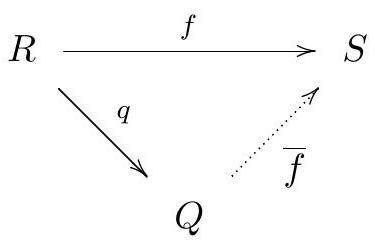
\includegraphics[max width=\textwidth, center]{2025_06_13_6ba93caed1e95a95104eg-062}\\
kommutiert, und $\bar{f}$ ist der einzige Homomorphismus $Q \rightarrow S$, für den das gilt.\\
Bemerkung 7.17. Wie in Proposition 5.10 im Fall von Gruppen zeigt man die Eindeutigkeit von Quotienten (sofern sie existieren!) bis auf Isomorphismus, der darüberhinaus selbst eindeutig ist, wenn er mit der Quotientenabbildung verträglich ist.

Satz 7.18 (Quotienten). Seien $R$ ein Ring und $I \subseteq R$ ein Ideal. Dann ist der Faktorring $R / I$ zusammen mit der kanonischen Projektion $p: R \rightarrow R / I$ ein Quotient.

Beweis. Das geht genauso wie im Satz 5.11 im Fall von Gruppen.\\
Bemerkung 7.19. Aus Satz 7.18 folgt, daß aufgrund der Eindeutigkeit des Quotienten, Bemerkung 7.17, die Quotientenabbildungen $q: R \rightarrow Q$ für Ideale $I \subseteq R$ immer surjektiv sind und $\operatorname{ker}(q)=I$ gilt. Das folgt nicht aus der definierenden universellen Eigenschaft des Quotienten, sondern aus der Konstruktion mittels Faktorring und der Eindeutigkeit.

Proposition 7.20. Sei $f: R \rightarrow S$ ein Ringhomomorphismus.\\
(1) $\quad$ Sei $I \subseteq S$ ein Ideal. Dann ist $f^{-1}(I)$ ein Ideal in $R$.\\
(2) Sei $f$ surjektiv und $I \subseteq R$ ein Ideal. Dann ist $f(I)$ ein Ideal in $S$.

Beweis. Das geht genauso wie in Proposition 5.7 im Fall von Gruppen:\\
(1) Es gilt $f^{-1}(I)=\operatorname{ker}(R \rightarrow S \rightarrow S / I)$.\\
(2) Das Bild $f(I)$ ist eine Untergruppe von $S$. Für alle $b \in S$ gibt es ein $a \in R$ mit $b=f(a)$. Daher gilt auch $b f(I)=f(a) f(I)=f(a I) \subseteq f(I)$.\\
Satz 7.21 (Homomorphiesatz). Sei $f: R \rightarrow S$ ein Ringhomomorphismus. Dann induziert $f$ einen Isomorphismus

$$
\bar{f}: R / \operatorname{ker}(f) \xrightarrow{\sim} \operatorname{im}(f), \quad \bar{f}(a+I):=f(a)
$$

Beweis. Der Beweis folgt analog zum Homomorphiesatz für Gruppen, Satz 5.15, aus der Quotienteneigenschaft von $R / I$, siehe Satz 7.18.

Man kann auch sagen, daß $\bar{f}$ als Abbildung der zugrundeliegenden Gruppen wegen Satz 5.15 existiert und ein Isomorphismus von Gruppen ist. Weiter ist die Multiplikation auf $R / I$ aber genau so definiert, daß $\bar{f}$ sogar ein Ringhomomorphismus und damit Ringisomorphismus ist.

Beispiel 7.22. Die Struktur eines Faktorrings $R / I$ bestimmt man am besten, indem man einen Isomorphismus $S \simeq R / I$ rät, den entsprechenden surjektiven Homomorphismus $f: R \rightarrow S$ hinschreibt und dann $I=\operatorname{ker}(f)$ nachweist. Mit dieser Methode bestimmen wir

$$
\mathbb{Z}[X] /(2, X) \simeq \mathbb{F}_{2}
$$

Der surjektive Homomorphismus $\mathbb{Z}[X] \rightarrow \mathbb{F}_{2}$ ist die Auswertung $X \mapsto 0 \in \mathbb{F}_{2}$ und auf Koeffizienten die kanonische Projektion $\mathbb{Z} \rightarrow \mathbb{Z} / 2 \mathbb{Z}=\mathbb{F}_{2}$. In der Tat sind 2 und $X$ im Kern der Auswertung, und genauer $f(0)=0 \bmod 2$ genau dann, wenn der konstante Koeffizient von $f$ gerade ist. Dies beschreibt das Ideal $(2, X)$.\\
Beispiel 7.23. Aus Satz 6.28 bekommen wir zu $\mathbb{R} \subseteq \mathbb{C}$ einen Ringhomomorphismus

$$
\mathbb{R}[X] \rightarrow \mathbb{C}, \quad X \mapsto i
$$

die Auswertung in $i \in \mathbb{C}$. Dieser Homomorphismus ist surjektiv mit Kern ( $X^{2}+1$ ), woraus sich nach dem Homomorphiesatz der folgende Isomorphismus ergibt:

$$
\mathbb{R}[X] /\left(X^{2}+1\right) \simeq \mathbb{C}
$$

Es lassen sich auch die Isomorphiesätze übertragen. Die Beweise sind formal die gleichen wie bei Gruppen, basierend auf dem Homomorphiesatz bzw. der Quotienteneigenschaft der Faktorringe.\\
Satz 7.24 (Erster Isomorphiesatz). Sei $U \subseteq R$ ein Unterring und $I \subseteq R$ ein Ideal.\\
Dann ist $U \cap I$ ein Ideal in $U$ und

$$
\begin{aligned}
U /(U \cap I) & \xrightarrow{\sim}(U+I) / I \\
u+(U \cap I) & \mapsto u+I
\end{aligned}
$$

ist ein Isomorphismus.\\
Beweis. Das ist der Homomorphiesatz für den Homomorphismus $U \rightarrow R \rightarrow R / I$.\\
Satz 7.25 (Zweiter Isomorphiesatz). Sei $R$ ein Ring und seien $I \subseteq J$ Ideale in R. Dann ist

$$
\begin{aligned}
(R / I) /(J / I) & \xrightarrow{\sim} R / J \\
(a+I)+J & \mapsto a+J
\end{aligned}
$$

ein Ringisomorphismus. Insbesondere ist $J / I$ ein Ideal in $R / I$.\\
Beweis. Das ist der Homomorphiesatz für den Ringhomomorphismus $R / I \rightarrow R / J$, der durch die Quotienteneigenschaft von $R \rightarrow R / I$ induziert wird.\\
Beispiel 7.26. Sei $K$ ein Körper. Wir betrachten im Ring $K[X, Y]$ das Ideal $J=\left(X-Y^{3}, Y-2\right)$. Zunächst liefert die Auswertung in $y=2$ einen (offensichtlich surjektiven) Ringhomomorphismus

$$
K[X, Y] \rightarrow K[X], \quad X \mapsto X, Y \mapsto 2,
$$

also nach dem Homomorphiesatz einen Isomorphismus $K[X, Y] /(Y-2) \simeq K[X]$. Es ist $I=$ $(Y-2) \subseteq J$ und $J / I$ wird in $K[X]$ zum Ideal $(X-8)$. Nach dem zweiten Isomorphiesatz ist dann

$$
K[X, Y] /\left(X-Y^{3}, Y-2\right) \simeq K[X] /(X-8)
$$

Eine erneute Anwendung des Homomorphiesatzes angewandt auf die Auswertung in $x=8$ führt zu $K[X] /(X-8) \simeq K$.\\
7.3. Algebraische Geometrie von Mengen. Algebraische Geometrie beschreibt die „Geometrie $X^{\prime \prime}$ durch die Algebra des Funktionenrings (algebraischer) Funktionen auf $X$. Wir skizzieren in diesem Abschnitt einen Babyfall hiervon.\\
Definition 7.27. Sei $X$ eine Menge und $K$ ein Körper.\\
(1) Für eine Teilmenge $Y \subseteq X$ definieren wir das Ideal im Ring der $K$-wertigen Funktionen $\operatorname{Abb}(X, K)$

$$
I(Y)=\{f \in \operatorname{Abb}(X, K) ; f(y)=0 \text { für alle } y \in Y\} .
$$

Dies ist der Kern der Einschränkung

$$
\operatorname{Abb}(X, K) \rightarrow \operatorname{Abb}(Y, K),\left.\quad f \mapsto f\right|_{Y}
$$

und daher ein Ideal.\\
(2) Umgekehrt setzen wir für ein Ideal $I \subseteq \operatorname{Abb}(X, K)$ die folgende Notation für die gemeinsame Nullstellenmenge (vanishing locus) fest:

$$
V(I)=\{x \in X ; f(x)=0 \quad \forall f \in I\}
$$

(3) Die charakteristische Funktion einer Teilmenge $Y \subseteq X$ ist die Funktion

$$
\mathbf{1}_{Y}(x)= \begin{cases}1 & x \in Y \\ 0 & x \notin Y\end{cases}
$$

Für einen Punkt (Element) $y \in Y$ setzen wir

$$
\mathbf{1}_{y}=\mathbf{1}_{\{y\}}
$$

also ist $\mathbf{1}_{y}: X \rightarrow K$ die Funktion mit

$$
\mathbf{1}_{y}(x)= \begin{cases}1 & y=x \\ 0 & y \neq x\end{cases}
$$

Algebraische Geometrie basiert auf den Eigenschaften der Übersetzung von Idealen in Teilmengen und umgekehrt.\\
Lemma 7.28. Die Konstruktionen $I(-)$ und $V(-)$ haben die folgenden Eigenschaften:\\
(1) Für Ideale $I \subseteq J$ von $\operatorname{Abb}(X, K)$ folgt $V(J) \subseteq V(I)$.\\
(2) Für Teilmengen $Y \subseteq Z$ von $X$ folgt $I(Z) \subseteq I(Y)$.\\
(3) $V(\operatorname{Abb}(X, K))=\emptyset$ und $V((0))=X$.\\
(4) $I(X)=(0)$ und $I(\emptyset)=\operatorname{Abb}(X, K)$.

Beweis. Sofort aus der Definition.\\
Eine Babyversion des "Nullstellensatzes" lautet für Mengen wie folgt.\\
Satz 7.29. Sei $X$ eine Menge und $K$ ein Körper.\\
(1) Sei $Y \subseteq X$ eine Teilmenge. Dann gilt $Y=V(I(Y))$. Die Zuordnung

$$
V:\{Y ; Y \subseteq X \text { Teilmenge }\} \rightarrow\{I ; I \subseteq \operatorname{Abb}(X, K) \text { Ideal }\}
$$

ist ein Linksinverses zur Zuordnung

$$
I:\{I ; I \subseteq \operatorname{Abb}(X, K) \text { Ideal }\} \rightarrow\{Y ; Y \subseteq X \text { Teilmenge }\}
$$

(2) Sei $\mathfrak{a} \subseteq \mathrm{Abb}(X, K)$ ein Ideal. Dann gilt $\mathfrak{a} \subseteq I(V(\mathfrak{a}))$.\\
(3) Wenn $X$ eine endliche Menge ist, dann gilt für jedes Ideal $\mathfrak{a} \subseteq \operatorname{Abb}(X, K)$ sogar

$$
\mathfrak{a}=I(V(\mathfrak{a})) .
$$

Die Zuordnungen $\mathfrak{a} \mapsto V(\mathfrak{a})$ und $Y \mapsto I(Y)$ sind zueinander inverse Bijektionen

$$
\{Y ; Y \subseteq X \text { Teilmenge }\} \stackrel{\sim}{\longleftrightarrow}\{\mathfrak{a} ; \mathfrak{a} \subseteq \operatorname{Abb}(X, K) \text { Ideal }\}
$$

Beweis. (1) Sei $Z=X \backslash Y$ das Komplement. Es ist $\mathbf{1}_{Z} \in I(Y)$ und daher

$$
V(I(Y)) \subseteq\left\{x \in X ; \mathbf{1}_{Z}(x)=0\right\}=Y
$$

Die andere Inklusion $Y \subseteq V(I(Y))$ gilt, weil $f(y)=0$ für alle $y \in Y$ und $f \in I(Y)$.\\
(2) Die Inklusion $\mathfrak{a} \subseteq I(V(\mathfrak{a}))$ folgt, weil $f(y)=0$ für alle $f \in \mathfrak{a}$ und $y \in V(\mathfrak{a})$.\\
(3) Sei $Y=V(\mathfrak{a})$. Dann gibt es für jedes $z \in Z=X \backslash Y$ ein $f \in \mathfrak{a}$ mit $f(z) \neq 0$. Mit $a=f(z)$ und $a^{-1}$ als konstante Funktion auf $X$ mit Wert $a^{-1}$ ist dann

$$
\mathbf{1}_{z}=a^{-1} \cdot \mathbf{1}_{z} \cdot f \in \mathfrak{a}
$$

Weil $Z$ endlich ist (die Summe hat dann nur endlich viele Summanden und ist wohldefiniert), gilt für alle $f \in I(Y)$

$$
f=\sum_{z \in Z} f(z) \cdot \mathbf{1}_{z}
$$

Dies zeigt mit (2)

$$
\mathfrak{a} \subseteq I(V(\mathfrak{a}))=I(Y) \subseteq\left(\mathbf{1}_{z} ; z \in Z\right) \subseteq \mathfrak{a}
$$

Korollar 7.30. Sei $X$ eine endliche Menge und $K$ ein Körper. Die Punkte $x \in X$ sind in Bijektion mittels $\mathfrak{a} \mapsto V(\mathfrak{a})$ und $Y \mapsto I(Y)$ zu den bezüglich Inklusion maximalen Idealen $\mathfrak{m} \subseteq$ $\operatorname{Abb}(X, K)$ mit $\mathfrak{m} \neq \operatorname{Abb}(X, K)$.

Beweis. Dies folgt sofort aus der Bijektion von Satz 7.29 (3) und der Beschreibung in Lemma 7.28, wie diese Bijektionen mit der Inklusionsrelation umgehen.

\section*{Übungsaufgaben zu §7}
Übungsaufgabe 7.1. Sei $K$ ein Körper. Sei $\mathfrak{a} \subseteq \operatorname{Abb}(\mathbb{N}, K)$ die Teilmenge (der Funktionen mit endlichem Träger)

$$
\mathfrak{a}=\{f: \mathbb{N} \rightarrow K ; \exists n \in \mathbb{N}: f(i)=0 \text { für alle } i>n\} .
$$

Zeigen Sie, daß $\mathfrak{a}$ ein Ideal im $\operatorname{Ring} \operatorname{Abb}(\mathbb{N}, K)$ ist und nicht $\mathfrak{a}=I(V(\mathfrak{a}))$ gilt.\\
Übungsaufgabe 7.2. Sei $K$ ein Körper und sei $h: X \rightarrow Y$ eine Abbildung von Mengen. Sei $h^{*}: \operatorname{Abb}(Y, K) \rightarrow \operatorname{Abb}(X, K)$ der entsprechende Pullback-Homomorphismus $f \mapsto h^{*}(f)=f \circ h$.\\
(1) Zeigen Sie: Für $f \in \operatorname{Abb}(Y, K)$ und $x \in X$ gilt mit $y=h(x)$ und $g=h^{*}(f)$ :

$$
g(x)=f(y)
$$

(2) Sei $Z \subseteq X$ eine Teilmenge. Bestimmen Sie $V(J) \subseteq Y$ für das Ideal

$$
J=\left(h^{*}\right)^{-1} I(Z) \subseteq \operatorname{Abb}(Y, K)
$$

\section*{Hauptidealringe}
8.1. Integritätsringe und Hauptidealringe. Den Körpern am nächsten kommen die Integritätsringe.

Lemma-Definition 8.1. Ein Integritätsring ist ein Ring mit $1 \neq 0$, in dem die folgenden äquivalenten Bedingungen gelten.\\
(a) Die Kürzungsregel gilt, d.h. für alle $a, x, y \in R$ mit $a \neq 0$ gilt

$$
a x=a y \quad \Longrightarrow \quad x=y .
$$

(b) Der Ring ist nullteilerfrei, d.h. für alle $x, y \in R$ gilt

$$
x y=0 \quad \Longrightarrow \quad x=0 \text { oder } y=0
$$

Beweis. Es gelte die Kürzungsregel und sei $x y=0$. Wenn $x=0$ ist nichts zu tun. Ansonsten gilt $x y=0=x 0$ und man kann wegen $x \neq 0$ zu $y=0$ kürzen.

Umgekehrt sei $R$ nun nullteilerfrei. Wenn $a \neq 0$, so folgt aus $a x=a y$, also $a(x-y)=0$, schon $x-y=0$ oder eben $x=y$. Das zeigt die Kürzungsregel.

Beispiel 8.2. (1) Ein Körper ist ein Integritätsring: Sei $K$ ein Körper, $a, x, y \in K$ mit $a x=a y$ und $a \neq 0$. Dann gibt es $a^{-1} \in K$ und so

$$
x=a^{-1}(a x)=a^{-1}(a y)=y
$$

Also erfüllt $K$ die Kürzungsregel. Die weitere Bedingung $0 \neq 1$ erfüllt ein Körper ebenfalls per Definition.\\
(2) Jeder Unterring eines Integritätsrings erbt die Kürzungsregel, zum Beispiel jeder Unterring eines Körpers wie etwa $\mathbb{Z} \subseteq \mathbb{Q}$. Dies ist kein Zufall, wie Satz A. 1 zeigt.\\
(3) Sei $R$ ein Ring mit $1 \neq 0$, und es habe die Menge $X$ mindestens 2 Elemente $x_{1} \neq x_{2}$. Dann ist $\operatorname{Abb}(X, R)$ kein Integritätsring. Sei dazu für $i=1,2$ die Funktion $f_{i}: X \rightarrow R$ mit

$$
f_{i}(x)= \begin{cases}1 & x=x_{i} \\ 0 & x \neq x_{i}\end{cases}
$$

Dann gilt $f_{1} \cdot f_{2}=0$, aber beide $f_{i}$ sind von 0 verschieden.\\
Die nach den Körpern einfachsten Ringe sind die Hauptidealringe.\\
Definition 8.3. (1) Ein Hauptideal ist ein Ideal $I$ in einem Ring $R$, das von einem Element erzeugt werden kann: es gibt $a \in R$ mit

$$
I=(a)=\{r a ; r \in R\}=R a
$$

(2) Ein Hauptidealring ist ein Integritätsring, in dem alle Ideale Hauptideale sind.

Beispiel 8.4. (1) Das typische Beispiel ist $\mathbb{Z}$. Ideale sind Untergruppen und damit von der Form ( $n$ ), also Hauptideale.\\
(2) Jeder Körper ist ein langweiliges Beispiel. Dort gibt es einfach keine nichttrivialen Ideale. Die trivialen Ideale sind stets Hauptideale.\\
(3) Sei $K$ ein Körper. Der Polynomring $K[X]$ ist ein Hauptidealring. Dies ist aus der Linearen Algebra bekannt, und wird hier mit Korollar 8.12 nochmals bewiesen.\\
(4) Das Ideal $(2, X) \subseteq \mathbb{Z}[X]$ ist kein Hauptideal. Angenommen, $(2, X)=(f)$, dann gibt es $g, h \in \mathbb{Z}[X]$ mit $2=g f$ und $X=h f$. Betrachtet man $f$ als Polynom in $\mathbb{Q}[X]$, so muß es wegen $2=g f$ konstant sein, und zwar $f= \pm 1$ wegen $X=h f$. Dann aber erzeugt $f$ schon das triviale Ideal $R$, Widerspruch. Insbesondere ist $\mathbb{Z}[X]$ kein Hauptidealring.\\
(5) Sei $R$ ein Ring. Das Ideal $I=(X, 1-X)$ im Polynomring $R[X]$ ist ein Hauptideal, denn wegen

$$
1=X+(1-X)
$$

ist $1 \in I$, und damit $R[X]=(1) \subseteq I \subseteq R[X]$. Folglich gilt $I=(1)$.\\
Bemerkung 8.5. Es gibt einen Dimensionsbegriff für kommutative Ringe mit dem Folgendes gilt:

\begin{itemize}
  \item Körper sind genau die Integritätsringe von Dimension 0.
  \item Hauptidealringe sind Integritätsringe von Dimension 1, und zwar genau die ohne Singularitäten und ohne nicht-triviale Geradenbündel und jedes Ideal ist endlich erzeugt.
  \item Der Ring $\mathbb{Z}[X]$ hat beispielsweise die Dimension 2.\\
8.2. Euklidische Ringe. Wir formalisieren den Beweis, daß $\mathbb{Z}$ ein Hauptidealring ist, indem wir Division mit Rest abstrahieren.
\end{itemize}

Definition 8.6. Eine euklidische Gradfunktion auf einem Ring $R$ ist eine Abbildung

$$
\delta: R \backslash\{0\} \rightarrow \mathbb{N}_{0}
$$

so daß es für alle $a \in R$ und $0 \neq d \in R$ Elemente $q, r \in R$ gibt mit\\
(i) $a=q d+r$,\\
(ii) $\quad r=0$ oder $\delta(r)<\delta(d)$.

Ein euklidischer Ring ist ein Integritätsring, den man mit einer euklidischen Gradfunktion versehen kann.

Beispiel 8.7. Die ganzen Zahlen $\mathbb{Z}$ sind ein euklidischer Ring mit der euklidischen Gradfunktion $\delta(n)=|n|$, dem reellen Absolutbetrag $|\cdot|$.\\
Satz 8.8. Sei $K$ ein Körper.\\
(1) Für alle $f, g \in K[X] \backslash\{0\}$ gilt $f g \neq 0$ und

$$
\operatorname{deg}(f g)=\operatorname{deg}(f)+\operatorname{deg}(g)
$$

Insbesondere ist der Polynomring $K[X]$ ein Integritätsring.\\
(2) Die Einheiten des Polynomrings sind $K[X]^{\times}=K^{\times}$als konstante Polynome $\neq 0$.

Beweis. (1) Sei $n=\operatorname{deg}(f)$ und $m=\operatorname{deg}(g)$. Dann ist $f=a_{n} X^{n}+$ Terme kleineren Grades und $g=b_{m} X^{m}+$ Terme kleiner Grades und $a_{n}, b_{m} \in K^{\times}$. Dann ist

$$
f g=a_{n} b_{m} X^{n+m}+\text { Terme kleineren Grades. }
$$

Weil $a_{n} b_{m} \neq 0$, folgt insbesondere $f g \neq 0$ und $\operatorname{deg}(f g)=n+m$.\\
(2) Wenn $f \in K[X]^{\times}$, dann gibt es $g \in K[X]$ mit $f g=1$. Es folgt aus (1), daß $0=\operatorname{deg}(f g)=$ $\operatorname{deg}(f)+\operatorname{deg}(g)$, somit $\operatorname{deg}(f)=0$ und $f$ ist konstant.\\
Satz 8.9. Sei $K$ ein Körper. Dann ist der Polynomring $K[X]$ mit dem Grad als euklidischer Gradfunktion ein euklidischer Ring.

Beweis. Mit $f, g \in K[X]$ verschieden von 0 ist $f g \neq 0$, weil nach Satz 8.8 ja $\operatorname{deg}(f g)=\operatorname{deg}(f)+$ $\operatorname{deg}(g)$ gilt. Insbesondere ist $K[X]$ ein Integritätsring.

Der Nachweis der Division mit Rest basiert auf dem Algorithmus der Polynomdivision. Zu $0 \neq d \in K[X]$ und jedem $f \in K[X]$ müssen wir $q, r \in K[X]$ finden mit

$$
f=q d+r
$$

und $r=0$ oder $\operatorname{deg}(r)<\operatorname{deg}(d)$. Für $f=0$ wählen wir $q=r=0$ und sind fertig. Wir nehmen daher im Folgenden $f \neq 0$ an.

Wir zeigen die Behauptung per Induktion nach $\operatorname{deg}(f)$. Falls $\operatorname{deg}(f)<\operatorname{deg}(d)$, so wählen wir $q=0$ und $r=f$, fertig. Wenn $m=\operatorname{deg}(f) \geq n=\operatorname{deg}(d)$, so schreiben wir

$$
\begin{aligned}
& f=a_{m} X^{m}+\ldots \text { Terme kleineren Grades } \\
& d=b_{n} X^{n}+\ldots \text { Terme kleineren Grades }
\end{aligned}
$$

mit $a_{m} \neq 0 \neq b_{n}$. Dann ist

$$
\begin{aligned}
\tilde{f} & =f-\frac{a_{m}}{b_{n}} X^{m-n} d \\
& =a_{m} X^{m}-\frac{a_{m}}{b_{n}} X^{m-n} \cdot b_{n} X^{n}+\ldots \text { Terme vom Grad }<m \\
& =\text { Terme vom Grad }<m
\end{aligned}
$$

also

$$
\operatorname{deg}(\tilde{f})<\operatorname{deg}(f)
$$

Per Induktionsannahme gibt es nun $\tilde{q}, \tilde{r}$ mit $\tilde{f}=\tilde{q} d+\tilde{r}$ und $\tilde{r}=0$ oder $\operatorname{deg}(\tilde{r})<\operatorname{deg}(d)$. Wir setzen dann

$$
\begin{aligned}
q & =\tilde{q}+\frac{a_{m}}{b_{n}} X^{m-n} \\
r & =\tilde{r}
\end{aligned}
$$

und rechnen

$$
f=\tilde{f}+\frac{a_{m}}{b_{n}} X^{m-n} d=\tilde{q} d+\tilde{r}+\frac{a_{m}}{b_{n}} X^{m-n} d=\left(\tilde{q}+\frac{a_{m}}{b_{n}} X^{m-n}\right) d+\tilde{r}=q d+r
$$

Weiterhin erfüllt das Restglied $r$ die geforderten Eigenschaften.\\
Jetzt kümmern wir uns um den Induktionsanfang: $\operatorname{deg}(f)=0$. Wenn $\operatorname{deg}(f)<\operatorname{deg}(d)$, dann ist wie oben nichts zu tun. Es fehlt also nur der Fall $\operatorname{deg}(f)=\operatorname{deg}(d)=0$. Da $d \neq 0$ gibt es also $d^{-1} \in K[X]$ und die Wahl $q=f d^{-1}$ mit $r=0$ erfüllt die Anforderungen.

Beispiel 8.10. Das folgende Beispiel zeigt, wie man die Existenz von Nullstellen erzwingen kann.\\
(1) Sei $K$ ein Körper und $f(X)=\sum_{i=0}^{n} a_{i} X^{i} \in K[X]$ ein Polynom positiven Grades $n=$ $\operatorname{deg}(f)$. Mittels eines Faktorrings kann man eine Nullstelle von $f$ erzwingen. Sei $I=(f(X))$ und $L=K[X] / I$. Die Inklusion der Konstanten gefolgt von der Quotientenabbildung

$$
K \subseteq K[X] \rightarrow L=K[X] / I
$$

Übungsaufgaben zu §8\\
Übungsaufgabe 8.1. Sei $R$ ein Integritätsring. Bestimmen Sie die Einheitengruppe im Polynomring $R[X]$ und im Potenzreihenring $R[[X]]$.\\
Übungsaufgabe 8.2. Sei $K$ ein Körper. Zeigen Sie, daß $K[[X]]$ ein Hauptidealring ist. Gibt es eine euklidische Gradfunktion auf $K[[X]]$ ?\\
Übungsaufgabe 8.3. Wir betrachten den Unterring $R \subseteq K[[X]]$ aus Aufgabe 6.6 bestehend aus allen Potenzreihen $f$ mit verschwindendem linearen Term. Zeigen Sie, daß das Ideal ( $X^{2}, X^{3}$ ) von $R$ kein Hauptideal in $R$ ist.

\section*{Arithmetik in Hauptidealringen}
9.1. Teilbarkeit in Integritätsringen. Wir vergeben einen Namen für die Situation, in der sich zwei Ringelemente multiplikativ um eine Einheit unterscheiden.

Definition 9.1. Sei $R$ ein Ring. Wir sagen Elemente $a, b \in R$ sind assoziiert, wenn

$$
a \sim b: \Longleftrightarrow \exists \varepsilon \in R^{\times} \text {mit } a=\varepsilon b .
$$

Lemma 9.2. Assoziiert zu sein ist eine Äquivalenzrelation.\\
Beweis. Das ist eine einfache Übungsaufgabe.\\
Über den Unterschied zwischen Elementen und den davon erzeugten Hauptidealen gibt die folgende Proposition Auskunft.\\
Proposition 9.3. Sei $R$ ein Ring und $a, b \in R$.\\
(1) Wenn $a \sim b$ ( $a$ assoziiert $z u b$ ), dann ist $(a)=(b)$.\\
(2) $a \in R^{\times} \Longleftrightarrow(a)=R$.\\
(3) Sei $R$ ein Integritätsring. Dann gilt $(a)=(b) \Longleftrightarrow a \sim b$.

Beweis. (1) Wenn $a \sim b$, dann gibt es $\varepsilon \in R^{\times}$und $a=\varepsilon b$. Aber dann ist

$$
(a)=R a=R \varepsilon b \subseteq(b)
$$

Da assoziiert zu sein symmetrisch ist, folgt auch $(b) \subseteq(a)$.\\
(2) Es gilt per Definition und nach (1)

$$
a \in R^{\times} \Longleftrightarrow a \sim 1 \Longleftrightarrow(a)=(1) \Longleftrightarrow(a)=R .
$$

(3) Wegen (1) ist nur zu zeigen, daß mit $(a)=(b)$ die Elemente $a, b$ assoziiert sind. Sei $(a)=(b)$. Dann gibt es $\varepsilon, \delta \in R$ mit $a=\varepsilon b$ und $b=\delta a$. Es folgt

$$
a=\varepsilon b=\varepsilon(\delta a)=a(\varepsilon \delta)
$$

Nach der Kürzungsregel gilt $\varepsilon \delta=1$ und $\varepsilon$ ist eine Einheit, oder $a=0$. In letzterem Fall gilt dann aber auch $b=\delta a=0$. In jedem Fall folgt $a \sim b$.\\
Bemerkung 9.4. Nach Proposition 9.3 werden Äquivalenzklassen von Elementen bis auf Assoziiertheit gerade durch die zugehörigen Hauptideale beschrieben. Diesen Standpunkt nehmen wir im Folgenden häufiger unausgesprochen ein, und zwar immer wenn wir mit Hauptidfealen statt Elementen argumentieren.

Definition 9.5. Sei $R$ ein Integritätsring und $a, x \in R$. Dann sagt man $x$ teilt $a$ oder $x$ ist Teiler von $a$ und verwendet die Notation

$$
x \mid a,
$$

wenn eine (also alle) der folgenden offensichtlich äquivalenten Bedingungen erfüllt sind:

$$
\exists y \in R: a=x y \Longleftrightarrow a \in(x) \Longleftrightarrow(a) \subseteq(x) .
$$

Ansonsten schreiben wir $x \nmid a$, wenn $x$ kein Teiler von $a$ ist.

Beispiel 9.6. Für den Ring $R=\mathbb{Z}$ beschreibt Definition 9.5 die wohlbekannte Teilerrelation ganzer Zahlen.

Proposition 9.7 (Eigenschaften der Teilerrelation). Seien $a, a^{\prime}, b, c, x, x^{\prime}$ Elemente eines Integritätsrings R. Dann gilt:\\
(1) $1 \mid a$.\\
(2) $x \mid 0$.\\
(3) $x \mid 1 \Longleftrightarrow x \in R^{\times}$.\\
(4) Wenn $x \mid a$, dann gilt $x b \mid a b$. Und wenn $b \neq 0$, dann folgt aus $x b \mid$ ab auch $x \mid a$.\\
(5) $a \mid b$ und $b|c \Longrightarrow a| c$.\\
(6) Seien $a_{1}, \ldots, a_{n}$ Elemente von $R$. Dann folgt aus $x \mid a_{i}$ für alle $i$, daß für alle $b_{i} \in R$, für $1 \leq i \leq n$ auch

$$
x \mid b_{1} a_{1}+\ldots+b_{n} a_{n}
$$

(7) Sind $a \sim a^{\prime}$ und $x \sim x^{\prime}$ jeweils assoziiert, dann gilt

$$
x\left|a \Longleftrightarrow x^{\prime}\right| a^{\prime} .
$$

(8) $\quad(a \mid b$ und $b \mid a) \Longleftrightarrow(a)=(b) \Longleftrightarrow a \sim b$ sind assoziiert.

Beweis. (1) $\quad a \in(1)=R$.\\
(2) $0 \in(x)$.\\
(3) Proposition 9.3 (2).\\
(4) Wenn $x \mid a$, dann gibt es $y \in R$ mit $a=x y$. Dann auch $a b=x b y$, somit $x b \mid a b$. Wenn $b \neq 0$, zeigt die Kürzungsregel auch die umgekehrte Implikation.\\
(5) Nach Voraussetzung gibt es $x, y \in R$ mit $b=a x$ und $c=b y$. Dann ist $c=a(x y)$ und $a \mid c$.\\
(6) Es gibt $y_{i}$ mit $a_{i}=x y_{i}$ für alle $1 \leq i \leq n$. Dann gilt

$$
x \mid x\left(b_{1} y_{1}+\ldots+b_{n} y_{n}\right)=b_{1} a_{1}+\ldots+b_{n} a_{n}
$$

(7) Nach Proposition 9.3 gilt $(a)=\left(a^{\prime}\right)$ und $(x)=\left(x^{\prime}\right)$. Dann folgt

$$
x\left|a \Longleftrightarrow(a) \subseteq(x) \Longleftrightarrow\left(a^{\prime}\right) \subseteq\left(x^{\prime}\right) \Longleftrightarrow x^{\prime}\right| a^{\prime} .
$$

(8) Es gilt $a \mid b$ und $b \mid a$ genau dann, wenn $(b) \subseteq(a)$ und $(a) \subseteq(b)$, was äquivalent ist zu $(a)=(b)$. Dies ist nach Proposition 9.3 dasselbe wie $a \sim b$.

\subsection*{Primelemente und irreduzible Elemente.}
Definition 9.8. Ein Element $a \neq 0$ eines Rings $R$ heißt irreduzibel, wenn\\
(i) $\quad a$ keine Einheit ist und\\
(ii) aus $a=x y$ für $x, y \in R$ folgt $x \in R^{\times}$oder $y \in R^{\times}$.

Beispiel 9.9. (1) Die positiven irreduziblen Elemente von $\mathbb{Z}$ sind genau die Primzahlen (per Definition).\\
(2) Ein lineares Polynom $X-a \in K[X]$ ist irreduzibel, denn in einer Zerlegung $X-a=$ $f(x) g(X)$ hat einer der Faktoren Grad 0 und ist daher eine Einheit.\\
(3) Ein Polynom $f \in K[X]$ vom $\operatorname{Grad} \operatorname{deg}(f) \geq 2$ mit Nullstelle $a \in K$ ist nicht irreduzibel. Polynomdivision von $f$ durch $X-a$ liefert

$$
f=q(X-a)+r
$$

mit $r(a)=f(a)-q(a)(a-a)=0$. Da $r=0$ oder $\operatorname{deg}(r)<\operatorname{deg}(X-a)=1$, ist $r$ konstant und in jedem Fall 0. Damit hat $f$ den Faktor $X-a$ und

$$
\operatorname{deg}(q)=\operatorname{deg}(f)-\operatorname{deg}(X-a)=\operatorname{deg}(f)-1>0
$$

zeigt, daß $q \notin K[X]^{\times}$.

Definition 9.10. Ein Primelement ist ein Element $\pi \neq 0$ eines Rings $R$, das keine Einheit ist, und für alle $x, y \in R$

$$
\pi|x y \quad \Longrightarrow \quad \pi| x \quad \text { oder } \quad \pi \mid y .
$$

Man sagt dann auch, $\pi$ ist prim.\\
Bemerkung 9.11. Sind $p \sim q$ assoziierte Elemente in $R$, dann folgt aus Proposition 9.7 (7)

$$
p \text { ist Primelement } \Longleftrightarrow q \text { ist Primelement. }
$$

Für ein Primelement $p \in R$ und eine Einheit $u \in R^{\times}$ist damit auch $q=u p$ ein Primelement.\\
Proposition 9.12. Sei $R$ ein Integritätsring. Dann ist jedes Primelement irreduzibel.\\
Beweis. Sei $\pi$ ein Primelement und $\pi=x y$ eine beliebige Zerlegung. Dann gilt $\pi \mid x y$ und oBdA $\pi \mid x$. Es gibt also $z \in R$ mit $\pi z=x$. Dann ist $\pi z y=x y=\pi=\pi \cdot 1$ und Kürzen von $\pi$ zeigt $z y=1$. Damit ist $y$ eine Einheit.

Der folgende Satz und der Fall der Primelemente in $\mathbb{Z}$, nämlich der Primzahlen, rechtfertigt den Namen Primelement.

Satz 9.13. Seien $R$ ein Hauptidealring und $a \in R, a \neq 0, a \notin R^{\times}$. Dann sind äquivalent:\\
(i) $\quad a$ ist Primelement.\\
(ii) a ist irreduzibel.\\
(iii) $R /(a)$ ist ein Körper.\\
(iv) $R /(a)$ ist ein Integritätsring.

Beweis. Wir zeigen (i) $\Longrightarrow$ (ii) $\Longrightarrow$ (iii) $\Longrightarrow$ (iv) $\Longrightarrow$ (i). Dabei ist (i) $\Longrightarrow$ (ii) die Aussage von Proposition 9.12, und (iii) $\Longrightarrow$ (iv) ist trivial.\\
(ii) $\Longrightarrow$ (iii): Es ist $0 \neq 1$ in $R /(a)$, weil sonst $R /(a)=0$ nach Lemma 6.8, also $R=(a)$ und gleichbedeutend $a \in R^{\times}$nach Proposition 9.3.

Sei $0 \neq \bar{x}=x+(a) \in R /(a)$. Wir müssen ein Inverses zu $\bar{x}$ finden. Da $\bar{x} \neq 0$, gilt $x \notin(a)$, also ist ( $a, x$ ) echt größer als ( $a$ ). Da $R$ ein Hauptidealring ist, gibt es ein $b \in R$ mit

$$
(b)=(a, x)
$$

Damit gibt es ein $c \in R$ mit $a=b c$. Weil $a$ irreduzibel ist, muß einer der beiden Faktoren $b$ oder $c$ eine Einheit sein. Wenn $c \in R^{\times}$, dann gibt es einen Widerspruch durch

$$
(b)=\left(a c^{-1}\right)=(a) \subsetneq(a, x)=(b)
$$

Also muß $b \in R^{\times}$Einheit sein. Dann ist $R=(b)=(a, x)$ und es gibt $\alpha, y \in R$ mit

$$
1=\alpha a+y x
$$

Das bedeutet

$$
x y \equiv 1 \quad(\bmod (a))
$$

und damit gilt in $R /(a)$ (mit der Notation $\bar{y}=y+(a)$ ):

$$
\bar{x} \bar{y}=1 \in R /(a)
$$

Damit ist $\bar{y}$ das gesuchte Inverse zu $\bar{x}$.\\
(iv) $\Longrightarrow$ (i): Sei $R /(a)$ ein Integritätsring und $a \mid x y$. Wir setzen $\bar{x}=x+(a)$ und $\bar{y}=y+(a)$ für die Bilder in $R /(a)$. Dann ist in $R /(a)$

$$
\bar{x} \cdot \bar{y}=(x+(a))(y+(a))=x y+(a)=(a)=0 \in R /(a)
$$

Da $R /(a)$ nullteilerfrei ist, muß $\bar{x}=0$ oder $\bar{y}=0$ gelten. OBdA sei $\bar{x}=0$, also $x \in(a)$, also $a \mid x$. Damit ist $a$ ein Primelement.

Bemerkung 9.14. Wir brauchen Satz 9.13 im Beweis von Korollar 9.16, weil wir mit der traditionellen Definition einer Primzahl arbeiten, anstatt von Primelementen in $\mathbb{Z}$ zu sprechen. Beides ist äquivalent, erfordert aber den Satz 9.13.

Die Äquivalenz (i) $\Longleftrightarrow$ (ii) in Satz 9.13 geht im Spezialfall $R=\mathbb{Z}$, also der Primzahlen, auf Euklid zurück.

Beispiel 9.15. Das Polynom $X^{2}+1 \in \mathbb{R}[X]$ ist irreduzibel nach Satz 9.13, weil $\mathbb{R}[X] /\left(X^{2}+1\right) \simeq \mathbb{C}$ ein Körper ist nach Beispiel 7.23.

Korollar 9.16. Sei $n>0$ eine ganze Zahl. Der Ring $\mathbb{Z} / n \mathbb{Z}$ ist ein Körper genau dann, wenn $n$ eine Primzahl ist.

Beweis. Das folgt sofort aus Satz 9.13 und der Definition einer Primzahl.\\
Notation 9.17. Für eine Primzahl $p$ bezeichnen wir $\mathbb{Z} / p \mathbb{Z}$ der Deutlichkeit halber mit

$$
\mathbb{F}_{p}
$$

wenn wir den endlichen Körper und nicht nur die zugrundeliegende additive zyklische Gruppe meinen.

Korollar 9.18. Sei $K$ ein Körper und $f(X) \in K[X]$ ein irreduzibles Polynom. Dann ist

$$
L=K[X] /(f(X))
$$

ein Körper.\\
(1) Genauer ist $L$ ein Oberkörper von $K$ über die Einbettung $K \subseteq L$ durch die Restklassen konstanter Polynome.\\
(2) In L hat $f(X)$ die Nullstelle $\alpha \equiv X(\bmod f(X))$.\\
(3) Jede Restklasse $P+(f(X)) \in L=K[X] /(f(X))$ hat einen eindeutigen Repräsentanten $P \in K[X]$ vom Grad $\operatorname{deg}(P)<\operatorname{deg}(f)$ (mit der Konvention $\operatorname{deg}(0)=-\infty$.)\\
(4) Die Einschränkung der Multiplikation auf $K \times L \rightarrow L$ macht aus $L$ einen $K$-Vektorraum der Dimension $\operatorname{dim}_{K}(L)=\operatorname{deg}(f)$ mit den Restklassen zu

$$
1, X, X^{2}, \ldots, X^{\operatorname{deg}(f)-1}
$$

als Basis.\\
Beweis. (1) Das folgt sofort aus Satz 9.13 (ii) $\Longleftrightarrow$ (iii) und (2) wurde in Beispiel 8.10 behandelt. (3) folgt aus Division mit Rest in $K[X]$ aus dem Beweis von Satz 8.9 und in (4) ist die Verifikation der Vektorraumaxiome eine Übungsaufgabe. Die Beschreibung der Basis folgt sofort aus (3).\\
Beispiel 9.19. Das Polynom $f(X)=X^{2}+X+1 \in \mathbb{F}_{2}[X]$ ist irreduzibel. Ansonsten hätte $X^{2}+X+1$ einen Linearfaktor in $\mathbb{F}_{2}[X]$ und folglich eine Nullstelle in $\mathbb{F}_{2}$. Aber dies schließt man durch Ausprobieren aus: $f(0)=f(1)=1$. Der Körper

$$
\mathbb{F}_{4}=\mathbb{F}_{2}[X] /\left(X^{2}+X+1\right)
$$

hat 4 Elemente, denn Division mit Rest zeigt, daß jede Restklasse einen eindeutigen Vertreter in $\mathbb{F}_{2}[X]$ vom Grad $\leq 1$ hat. Davon gibt es 4 .

Man kann zu jeder Primzahl $p$ und einer Potenz $q=p^{d}$ ein irreduzibles Polynom $f \in \mathbb{F}_{p}[X]$ vom $\operatorname{Grad} d=\operatorname{deg}(f)$ finden, so daß

$$
\mathbb{F}_{q} \simeq \mathbb{F}_{p}[X] /(f)
$$

ein Körper mit $q$ Elementen ist. Man kann weiter zeigen, daß $\mathbb{F}_{q}$ bis auf Isomorphie eindeutig durch $q$ gegeben ist und die Mächtigkeit eines endlichen Körpers stets eine Primzahlpotenz sein muß. Damit hat man einen vollständigen Überblick über die Klassifikation endlicher Körper. Mehr dazu in der Vorlesung Algebra.\\
9.3. Die Eindeutigkeit der Primzerlegung in Hauptidealringen. Wir zerlegen zuerst als Produkt von irreduziblen Elementen, obwohl nach Satz 9.13 irreduzibel und prim in Hauptidealringen äquivalent sind, weil der Existenzbeweis mit der Eigenschaft ,irreduzibel‘ spielt.

Lemma 9.20. Sei $R$ ein Integritätsring und $a, x, y \in R$ mit $a=y x \neq 0$. Wenn $(a)=(x)$, dann ist $y \in R^{\times}$.

Beweis. Wegen $(a)=(x)$ gibt es $z \in R$ mit $x=a z$. Dann folgt $a=a(y z)$ und wegen $a \neq 0$ bereits $1=y z$. Dies zeigt $y \in R^{\times}$.

Den nächsten Satz könnte man als die Bestätigung der „Atomhypothese" in Hauptidealringen verstehen: jedes Element läßt sich multiplikativ in eine endliche Menge von unteilbaren (irreduziblen) Elementen zerlegen.

Satz 9.21. Sei $R$ ein Hauptidealring. Dann läßt sich jedes $0 \neq a \in R$ als Produkt einer Einheit und endlich vieler irreduzibler Elemente schreiben.

Beweis. Schritt 1: Wir betrachten die Menge der Gegenbeispiele

$$
\mathscr{M}=\left\{x \in R ; x \neq 0 \text { nicht der Form } x=u \cdot \prod_{i=1}^{n} p_{i} \text { mit } u \in R^{\times}, p_{i} \text { irreduzibel in } R\right\}
$$

und zeigen, daß $\mathscr{M}$ leer ist. Wir führen einen Widerspruchsbeweis und nehmen $\mathscr{M} \neq \emptyset$ an.\\
Schritt 2: Angenommen, es gibt unter den Hauptidealen $(x)$ zu $x \in \mathscr{M}$ kein bezüglich Inklusion maximales Ideal, dann gibt es echte unendlich aufsteigende Ketten

$$
\left(x_{1}\right) \subsetneq\left(x_{2}\right) \subsetneq \ldots \subsetneq\left(x_{i}\right) \subsetneq \ldots
$$

mit $x_{i} \in \mathscr{M}$ für alle $i \geq 1$. Da $R$ Hauptidealring ist, gibt es $x \in R$ mit

$$
(x)=\bigcup_{i \geq 1}\left(x_{i}\right)
$$

denn die Vereinigung ist nach Lemma 7.10 ein Ideal. Für hinreichend großes $j$ muß schon $x \in\left(x_{j}\right)$ gelten. Daraus folgt für $k>j$

$$
\bigcup_{i \geq 1}\left(x_{i}\right)=(x) \subseteq\left(x_{j}\right) \subsetneq\left(x_{k}\right) \subseteq \bigcup_{i \geq 1}\left(x_{i}\right)
$$

ein Widerspruch. Es gibt also bezüglich Inklusion der Hauptideale maximale Gegenbeispiele.\\
Schritt 3: Sei $a \in \mathscr{M}$ ein maximales Gegenbeispiel, d.h. für alle $(a) \subsetneq(y)$ gilt $y \notin \mathscr{M}$. Per Definition enthält $\mathscr{M}$ weder Einheiten (Fall $n=0$ ) noch irreduzible Elemente (Fall $n=1$ ). Somit ist $a$ weder Einheit noch irreduzibel. Dann ist $a$ ein Produkt von Nichteinheiten.

Sei also $a=x y$ eine nichttriviale Zerlegung mit $x, y \notin R^{\times}$. Dann ist $(a) \subsetneq(x)$ eine echte Inklusion, da sonst $y$ Einheit wäre nach Lemma 9.20. Entsprechend ist $(a) \subsetneq(y)$ eine echte Inklusion. Also sind $x, y \notin \mathscr{M}$. Es gibt daher Zerlegungen

$$
\begin{aligned}
& x=u \cdot p_{1} \cdot \ldots \cdot p_{n} \\
& y=v \cdot q_{1} \cdot \ldots \cdot q_{m}
\end{aligned}
$$

für irreduzible Elemente $p_{1}, \ldots, p_{n}, q_{1}, \ldots, q_{m}$ von $R$ und $u, v \in R^{\times}$. Daraus folgt die Zerlegung

$$
a=x y=(u v) \cdot p_{1} \cdot \ldots \cdot p_{n} \cdot q_{1} \cdot \ldots \cdot q_{m}
$$

im Widerspruch zu $a \in \mathscr{M}$. Es kann keine Gegenbeispiele zur Aussage des Satzes geben.\\
Bemerkung 9.22. Sei $K$ ein Körper. Im Polynomring $K[X]$ kann man Satz 9.21 leicht per Induktion über den Grad beweisen. Für $\operatorname{deg}(f) \leq 0$ handelt es sich um 0 oder eine Einheit. Für\\
$\operatorname{deg}(f)>0$ ist entweder $f$ irreduzibel, dann ist nach Satz $9.13 f$ prim und nichts zu tun. Andernfalls ist $f$ nicht irreduzibel und wir können $f=g h$ mit $g, h \notin K[X]^{\times}$schreiben. Nach Satz 8.8 folgt $\operatorname{deg}(g), \operatorname{deg}(h)>0$ und $\operatorname{deg}(f)=\operatorname{deg}(g)+\operatorname{deg}(h)$, also

$$
\operatorname{deg}(g), \operatorname{deg}(h)<\operatorname{deg}(f),
$$

und die Induktionsannahme findet auf $g, h$ Anwendung. Eine Zerlegung für $g$ und $h$ als Produkt irreduzibler Polynome kann man zu einer Faktorzerlegung von $f$ multiplizieren.

Der Satz über die Eindeutigkeit der Primfaktorzerlegung ist schon sehr alt (Euklid für $R=\mathbb{Z}$ ). In Hauptidealringen gilt der Satz allgemein. Nicht aber in beliebigen Ringen als Satz über eindeutige Faktorisierung in irreduzible Elemente, wie das klassische Beispiel in dem Unterring

$$
\mathbb{Z}[\sqrt{-5}]=\{a+b \sqrt{-5} ; a, b \in \mathbb{Z}\} \subseteq \mathbb{C}
$$

zeigt ${ }^{8}$ mit den zwei echt verschiedenen Faktorisierungen

$$
6=2 \cdot 3=(1+\sqrt{-5})(1-\sqrt{-5})
$$

Theorem 9.23 (Eindeutige Primfaktorzerlegung in Hauptidealringen). Sei $R$ ein Hauptidealring und $a \in R, a \neq 0$. Dann hat a eine Produktzerlegung

$$
a=u \cdot p_{1} \cdot \ldots \cdot p_{n}
$$

in Primelemente $p_{i}$ für $1 \leq i \leq n$ und eine Einheit $u$.\\
Die Zerlegung ist eindeutig bis auf Permutation und assoziierte Primelemente. Genauer, sei

$$
a=v \cdot q_{1} \cdot \ldots \cdot q_{m}
$$

eine zweite solche Faktorisierung mit $v \in R^{\times}$und $q_{j}$ prim für $1 \leq j \leq m$. Dann gilt $m=n$ und es gibt eine Permutation $\sigma \in S_{n}$, sowie Einheiten $\varepsilon_{i}$ mit

$$
q_{\sigma(i)}=\varepsilon_{i} p_{i}
$$

für alle $1 \leq i \leq n$ und $u=v \cdot \prod_{i=1}^{n} \varepsilon_{i}$.\\
Beweis. Nach Satz 9.13 suchen wir eine Produktzerlegung in irreduzible Faktoren. Die Existenz der Zerlegung folgt aus Satz 9.21.

Wir zeigen die Eindeutigkeit per Induktion nach $n$. Für $n=0$ ist $a=u \in R^{\times}$, somit muß für alle $1 \leq j \leq m$ in

$$
R=(a) \subseteq\left(q_{j}\right) \subseteq R
$$

Gleichheit gelten. Damit ist $q_{j}$ eine Einheit und nicht prim, Widerspruch zu $m>0$. Damit gilt die Aussage im Fall $n=0$.

Sei der Satz für $n-1$ bewiesen, und habe $a$ zwei Zerlegungen wie im Satz. Da

$$
p_{n} \mid a=v \cdot q_{1} \cdot \ldots \cdot q_{m}
$$

teilt $p_{n}$ einen der Faktoren. Aus $p_{n} \mid v$ würde $1 \in R=(v) \subseteq\left(p_{n}\right)$ folgen, und $p_{n}$ wäre Einheit. Also gilt $p_{n} \nmid v$, und es gibt ein $1 \leq j \leq m$ mit $p_{n} \mid q_{j}$. Nach Permutation ${ }^{9}$ der $q_{j}$ dürfen wir annehmen, daß $j=m$. Dann gibt es $\varepsilon_{n} \in R$ mit $q_{m}=\varepsilon_{n} p_{n}$. Da $q_{m}$ prim, also irreduzibel nach Satz 9.13, und $p_{n} \notin R^{\times}$ist, muß $\varepsilon_{n}$ eine Einheit sein. Wir betrachten

$$
b=a / q_{m}=\left(u \varepsilon_{n}^{-1}\right) \cdot p_{1} \cdot \ldots \cdot p_{n-1}
$$

\footnotetext{${ }^{8}$ Hier ist natürlich noch einiges zu zeigen: die Elemente 2,3 und $1 \pm \sqrt{-5}$ sind irreduzibel in $\mathbb{Z}[\sqrt{-5}]$, insbesondere keine Einheiten.\\
${ }^{9}$ Diese praktische Annahme erleichtert die Notation, sorgt aber eventuell für die irrige Annahme, daß in der gesuchten Permutation $\sigma(n)=n$ gilt. Dies haben wir in diesem Moment so organisiert. In der Ausgangsfaktorisierung gilt dies nicht. Wir verwenden hier die Gruppenstruktur der Permutationsgruppe $S_{n}$, indem wir zwei Permutationen hintereinander ausführen. Oder, wir verwenden, daß die Behauptung offensichtlich nach beliebiger Permutation der Faktoren bewiesen werden darf.
}
mit der zweiten Faktorisierung
$$
b=v \cdot q_{1} \cdot \ldots \cdot q_{m-1}
$$

Per Induktionsannahme gilt nun $n-1=m-1$, also $n=m$, und es gibt eine Permutation $\sigma^{\prime} \in S_{n-1}$ und Einheiten $\varepsilon_{i}$ mit den geforderten Eigenschaften für die Faktorisierungen von $b$. Setzen wir $\sigma^{\prime}$ zu $\sigma \in S_{n}$ fort durch $\sigma(n):=n$, dann folgt damit die Behauptung.

Bemerkung 9.24. Sei $R$ ein Hauptidealring. In der eindeutigen Primfaktorzerlegung nach Theorem 9.23 kann man Primelemente zu assoziierten Primelementen tauschen. Mit der Notation aus dem Theorem gilt für $\varepsilon \in R^{\times}$:

$$
u \cdot p_{1} \cdot \ldots \cdot p_{n}=\left(u p^{-1}\right) \cdot\left(\varepsilon p_{1}\right) \cdot \ldots \cdot p_{n}
$$

Dabei sagt uns Bemerkung 9.11, dass mit $p_{1}$ auch $\varepsilon p_{1}$ prim ist.\\
Um die Primfaktorzerlegung zu standardisieren, wählt man aus jeder Äquivalenzklasse von Primelementen bis auf Assoziiertheit, also bis auf Multiplikation mit einer Einheit, einen Vertreter aus, und nutzt nur diese ausgezeichneten Primelemente in der Primfaktorzerlegung. Beispielsweise

\begin{itemize}
  \item für $R=\mathbb{Z}$ kann man aus $\{ \pm p\}$ jeweils das Primelement $p>0$ wählen, also die positiven Primzahlen,
  \item für eine Körper $K$ und den Polynomring $R=K[X]$ sind die Einheiten $K^{\times}$und ein natürlicher Vertreter ist durch das eindeutige normierte Polynom (Leitkoeffizient 1) in der Äquivalenzklasse gegeben (durch Skalieren mit dem Inversen des Leitkoeffizienten).\\
Mit diesen Wahlen hat jedes $a \in R$ eine eindeutige Primfaktorzerlegung bis auf die Reihenfolge der Primfaktoren der Form
\end{itemize}

$$
a=u \cdot p_{1}^{e_{1}} \cdot \ldots \cdot p_{n}^{e_{n}}
$$

wobei $u \in R^{\times}$eine Einheit, $e_{1}, \ldots, e_{n}$ ganze Zahlen $\geq 1$ sind und die $p_{1}, \ldots, p_{n}$ aus der Liste der ausgezeichneten Primelemente stammen.

Definition 9.25. Ein faktorieller Ring ist ein Integritätsring $R$, in dem jedes $a \in R, a \neq 0$ eine eindeutige Primfaktorzerlegung im Sinne von Theorem 9.23 besitzt.

Korollar 9.26. Es gilt für einen Integritätsring:

$$
R \text { euklidisch } \Longrightarrow R \text { Hauptidealring } \Longrightarrow R \text { faktoriell. }
$$

Beweis. Theorem 8.11 und Theorem 9.23.\\
Bemerkung 9.27. Die umgekehrten Implikationen gelten nicht. Der Ring $\mathbb{R}[X, Y] /\left(X^{2}+Y^{2}+1\right)$ ist ein Hauptidealring, aber nicht euklidisch. Der Ring $\mathbb{Z}[X]$ ist ein faktorieller Ring, aber kein Hauptidealring.

\section*{Der Chinesische Restsatz}
10.1. Größter gemeinsamer Teiler und kleinstes gemeinsames Vielfaches. In Hauptidealringen kann man größte gemeinsame Teiler und kleinste gemeinsame Vielfache definieren.\\
Bemerkung 10.1. In $\mathbb{Z}$ bedeutet „groß" vermutlich, daß der Absolutbetrag groß ist. Im Polynomring $K[X]$ über einem Körper bedeutet „groß" vermutlich einen großen Grad. In allgemeinen Hauptidealringen gibt es eine solche Anschauung nicht. Aber es gibt die Teilbarkeitsrelation, und in dem Sinne wollen wir bei $x \mid a$ so tun als ob $a$ größer ist als sein Teiler $x$. Allerdings ist zu beachten, daß Teilbarkeit nur eine partielle Ordnung liefert: nicht alle Elemente sind vergleichbar. Zum Beispiel ist in $\mathbb{Z}$ in diesem Sinne nicht erklärt, ob 6 oder 10 größer ist.

Definition 10.2. Sei $R$ ein Integritätsring und seien $a_{1}, \ldots, a_{r} \in R$.\\
(1) Ein größter gemeinsamer Teiler (ggT) von $a_{1}, \ldots, a_{r}$ ist ein $d \in R$ mit\\
(i) $\quad d \mid a_{i}$ für alle $i=1, \ldots, r$, und\\
(ii) für jedes $t \in R$ mit $t \mid a_{i}$ für alle $i=1, \ldots, r$ gilt $t \mid d$.

Wir notieren den ggT als

$$
\operatorname{ggT}\left(a_{1}, \ldots, a_{r}\right)
$$

(2) Ein kleinstes gemeinsames Vielfaches (kgV) von $a_{1}, \ldots, a_{r}$ ist ein $v \in R$ mit\\
(i) $\quad a_{i} \mid v$ für alle $i=1, \ldots, r$, und\\
(ii) für jedes $w \in R$ mit $a_{i} \mid w$ für alle $i=1, \ldots, r$ gilt $v \mid w$.

Wir notieren das kgV als

$$
\operatorname{kgV}\left(a_{1}, \ldots, a_{r}\right)
$$

Proposition 10.3. Sei $R$ ein Integritätsring und seien $a_{1}, \ldots, a_{r} \in R$.\\
(1) Wenn ein größter gemeinsamer Teiler d der $a_{1}, \ldots, a_{r}$ existiert, dann ist $d^{\prime} \in R$ ein größter gemeinsamer Teiler $\Longleftrightarrow d \sim d^{\prime}$.\\
(2) Wenn ein kleinstes gemeinsames Vielfaches $v$ der $a_{1}, \ldots, a_{r}$ existiert, dann ist $v^{\prime} \in R$ ein kleinstes gemeinsames Vielfaches $\Longleftrightarrow v \sim v^{\prime}$.\\
Mit andern Worten: existierende ggT und $\mathrm{kg} V$ sind eindeutig bis auf Multiplikation mit einer Einheit.

Beweis. (1) Weil $d^{\prime}$ ein gemeinsamer Teiler ist, folgt $d \mid d^{\prime}$. Analog gilt $d^{\prime} \mid d$. Aus Proposition 9.7 (8) folgt dann $d \sim d^{\prime}$.

Wenn umgekehrt $d \sim d^{\prime}$, dann haben $d$ und $d^{\prime}$ die gleichen Teilbarkeitseigenschaften nach Proposition 9.7 (7).\\
(2) beweist man genauso wie (1).

Proposition 10.4. In einem Hauptidealring $R$ existieren zu beliebigen Elementen $a_{1}, \ldots, a_{r} \in R$ der ggT und das kgV. Genauer gilt:\\
(1) Ein $d \in R$ ist ein ggT von $a_{1}, \ldots, a_{r}$ genau dann, wenn

$$
(d)=\left(a_{1}, \ldots, a_{r}\right)
$$

(2) $\operatorname{Ein} v \in R$ ist ein $k g V$ von $a_{1}, \ldots, a_{r}$ genau dann, wenn

$$
(v)=\bigcap_{i=1}^{r}\left(a_{i}\right) .
$$

Beweis. Weil $R$ ein Hauptidealring ist, werden durch Erzeugnis und Schnitt Elemente $d, v \in R$ definiert, und zwar (wie zu erwarten) nur eindeutig bis auf assoziierte Elemente. Wir müssen zeigen, daß solche $d$ ein ggT und solche $v$ ein kgV sind. Aber das folgt sofort aus der Definition der Teilbarkeitsbeziehung:\\
(1) Es gilt $\left(a_{i}\right) \subseteq(d)$ für alle $i=1, \ldots, r$, also $d \mid a_{i}$. Für jedes $t \in R$ mit $\left(a_{i}\right) \subseteq(t)$ für alle $i=1, \ldots, r$, also $t \mid a_{i}$, folgt

$$
(d)=\left(a_{1}, \ldots, a_{r}\right) \subseteq(t), \quad \text { also } \quad t \mid d
$$

(2) Es gilt $(v) \subseteq\left(a_{i}\right)$ für alle $i=1, \ldots, r$, also $a_{i} \mid v$. Für jedes $w \in R$ mit $(w) \subseteq\left(a_{i}\right)$ für alle $i=1, \ldots, r$, also $a_{i} \mid w$, folgt

$$
(w) \subseteq \bigcap_{i=1}^{r}\left(a_{i}\right)=(v), \quad \text { also } \quad v \mid w
$$

Bemerkung 10.5. Man kann ggT und kgV als Ideale in jedem Ring durch die rechte Seite der Formeln aus Proposition 10.4 definieren. Die besser Definition betrachtet ggT und kgV nur als Ideale. Der Übergang zu Elementen bei Hauptidealringen führt zu Unbestimmtheit bis auf eine Einheit, siehe Proposition 9.3.

Korollar 10.6. Sei $R$ ein Hauptidealring und $a_{1}, \ldots, a_{n} \in R$. Für alle $1 \leq r \leq n$ gilt

$$
\begin{aligned}
& \operatorname{ggT}\left(a_{1}, \ldots, a_{n}\right)=\operatorname{ggT}\left(\operatorname{ggT}\left(a_{1}, \ldots, a_{r}\right), a_{r+1}, \ldots, a_{n}\right), \\
& \operatorname{kgV}\left(a_{1}, \ldots, a_{n}\right)=\operatorname{kgV}\left(\operatorname{kgV}\left(a_{1}, \ldots, a_{r}\right), a_{r+1}, \ldots, a_{n}\right) .
\end{aligned}
$$

Beweis. Das folgt sofort aus den Formeln aus Proposition 10.4 wegen der Idealgleichungen

$$
\begin{aligned}
\left(a_{1}, \ldots, a_{n}\right) & =\left(\left(a_{1}, \ldots, a_{r}\right), a_{r+1}, \ldots, a_{n}\right) \\
\bigcap_{i=1}^{n}\left(a_{i}\right) & =\bigcap_{i=1}^{r}\left(a_{i}\right) \cap\left(a_{r+1}\right) \cap \ldots \cap\left(a_{n}\right)
\end{aligned}
$$

Korollar 10.7 (Lemma von Bézout). Sei $R$ ein Hauptidealring und $d=\operatorname{ggT}\left(a_{1}, \ldots, a_{r}\right)$. Dann ist $d$ eine $R$-Linearkombination der $a_{i}$, d.h.

$$
d=x_{1} a_{1}+\ldots+x_{r} a_{r}
$$

für geeignete Elemente $x_{i} \in R$ für $1 \leq i \leq r$.\\
Beweis. Das ist nach der Formel aus Proposition 10.4 (1) klar.\\
Die Eindeutigkeit der Primfaktorzerlegung in einem Hauptidealring erlaubt es, den ggT und das kgV mit Hilfe der Primfaktorzerlegung auszudrücken.

Korollar 10.8. Seien $p_{i} \in R$ für $1 \leq i \leq n$ paarweise nicht-assoziierte Primelemente eines Hauptidealrings $R$.\\
(1) Sei $a=u \cdot p_{1}^{e_{1}} \cdot \ldots \cdot p_{n}^{e_{n}}$ mit $u \in R^{\times}$. Dann gilt für $b \in R$ :

$$
\begin{gathered}
b \mid a \Longleftrightarrow \text { es gibt } 0 \leq f_{i} \leq e_{i} \text { für } 1 \leq i \leq n \text { und } v \in R^{\times} \text {mit } b=v \cdot p_{1}^{f_{1}} \cdot \ldots \cdot p_{n}^{f_{n}} . \\
\text { Sei } a_{j}=u_{j} \cdot \prod_{i=1}^{n} p_{i}^{e_{i j}} \text { mit } u_{j} \in R^{\times} \text {und mit } e_{i j} \in \mathbb{N}_{0} \text { für alle } 1 \leq i \leq n \text { und } 1 \leq j \leq r . \text { Sei } \\
m_{i}=\min _{1 \leq j \leq r}\left\{e_{i j}\right\} \quad \text { und } \quad M_{i}=\max _{1 \leq j \leq r}\left\{e_{i j}\right\} .
\end{gathered}
$$

Dann gilt:

$$
\begin{aligned}
\operatorname{ggT}\left(a_{1}, \ldots, a_{r}\right) & =\prod_{i=1}^{n} p_{i}^{m_{i}} \\
\operatorname{kgV}\left(a_{1}, \ldots, a_{r}\right) & =\prod_{i=1}^{n} p_{i}^{M_{i}}
\end{aligned}
$$

Beweis. (1) Wir schreiben $a=b c$. Die Primfaktorzerlegungen von $b$ und $c$ legen wegen der Eindeutigkeit die Primfaktorzerlegung von $a$ fest: man multipliziere beide Zerlegungen. Aussage (2) folgt sofort aus Aussage (1).

Korollar 10.9. Sei $R$ ein Hauptidealring und seien $a, b \in R$. Dann gilt

$$
(\operatorname{ggT}(a, b) \cdot \operatorname{kgV}(a, b))=(a b)
$$

Beweis. Das folgt wegen

$$
m+M=\min \{m, M\}+\max \{m, M\}
$$

sofort aus den Formeln von Korollar 10.8. Der Übergang zu Hauptidealen ist nötig, weil ggT und kgV nur eindeutig bis auf assoziierte Elemente definiert sind.\\
10.2. Der euklidische Algorithmus in euklidischen Ringen. Seien $a, b \in R$ Elemente eines Hauptidealrings und $d=\operatorname{ggT}(a, b)$. Es ist besonders interessant, den ggT „algorithmisch" als $R$-Linearkombination

$$
d=s \cdot a+t \cdot b
$$

bestimmen zu können. Dies funktioniert für euklidische Ringe, sofern die Division mit Rest algorithmisch ist, wie etwa bei $\mathbb{Z}$ oder bei Polynomringen $K[X]$ über einem Körper $K$. Dies setzt natürlich voraus, daß auch das Rechnen in $K$ algorithmisch ist.

Algorithmus 10.10. Sei $\delta$ eine euklidische Gradfunktion auf $R$. Wir berechnen für $a, b \in R$

$$
d=\operatorname{ggT}(a, b) \quad \text { und } s, t \in R \text { mit } \quad d=s \cdot a+t \cdot b
$$

Initialisierung: Wir nehmen ohne Einschränkung an, daß $\delta(a) \geq \delta(b)$. Wir setzen

$$
r_{0}=a, \quad r_{1}=b \quad \text { und } \quad\left(\begin{array}{cc}
s_{0} & t_{0} \\
s_{1} & t_{1}
\end{array}\right)=\left(\begin{array}{cc}
1 & 0 \\
0 & 1
\end{array}\right) .
$$

Wir starten mit $i=1$.\\
Rekursion: Solange $r_{i} \neq 0$ gilt, berechnen wir per Division mit Rest $q_{i}$ und $r_{i+1}$ mit $\delta\left(r_{i+1}\right)<$ $\delta\left(r_{i}\right)$ oder $r_{i+1}=0$, so daß $r_{i-1}=q_{i} \cdot r_{i}+r_{i+1}$, also

$$
r_{i+1}=r_{i-1}-q_{i} \cdot r_{i}
$$

und setzen dann:

$$
\begin{aligned}
s_{i+1} & :=s_{i-1}-q_{i} s_{i} \\
t_{i+1} & :=t_{i-1}-q_{i} t_{i}
\end{aligned}
$$

Wenn wir zu einem Index $n$ kommen mit $r_{n+1}=0$, dann STOP:

$$
d:=r_{n}=s_{n} \cdot a+t_{n} \cdot b
$$

Zur Korrektheit des Algorithmus betrachten wir zunächst die Folge $r_{0}, r_{1}, r_{2}, \ldots$ Die Folge $\delta\left(r_{0}\right), \delta\left(r_{1}\right), \delta\left(r_{2}\right), \ldots$ ist streng monoton fallend in $\mathbb{N}_{0}$ und damit endlich. Wir erreichen daher nach endlich vielen Iterationen ein $n$ mit $r_{n+1}=0$. Wegen

$$
\left(\operatorname{ggT}\left(r_{i-1}, r_{i}\right)\right)=\left(r_{i-1}, r_{i}\right)=\left(r_{i-1}-q_{i} r_{i}, r_{i}\right)=\left(r_{i}, r_{i+1}\right)=\left(\operatorname{ggT}\left(r_{i}, r_{i+1}\right)\right)
$$

berechnet der Algorithmus, was er vorgibt zu berechnen (eigentlich nur bis auf ,assoziiert‘):

$$
\operatorname{ggT}(a, b)=\operatorname{ggT}\left(r_{0}, r_{1}\right)=\ldots=\operatorname{ggT}\left(r_{i-1}, r_{i}\right)=\ldots=\operatorname{ggT}\left(r_{n}, r_{n+1}\right)=\operatorname{ggT}(d, 0)=d
$$

Nun beweisen wir per Induktion für alle $i$

$$
\binom{r_{i-1}}{r_{i}}=\left(\begin{array}{cc}
s_{i-1} & t_{i-1} \\
s_{i} & t_{i}
\end{array}\right)\binom{a}{b} .
$$

Dies gilt für $i=1$ aufgrund der Initialisierung des Algortihmus

$$
\binom{r_{0}}{r_{1}}=\binom{a}{b}=\left(\begin{array}{ll}
1 & 0 \\
0 & 1
\end{array}\right)\binom{a}{b}=\left(\begin{array}{ll}
s_{0} & t_{0} \\
s_{1} & t_{1}
\end{array}\right)\binom{a}{b}
$$

Wenn es für $i$ gilt, dann auch für $i+1$ :

$$
\begin{aligned}
\binom{r_{i}}{r_{i+1}} & =\binom{r_{i}}{r_{i-1}-q_{i} r_{i}}=\left(\begin{array}{cc}
0 & 1 \\
1 & -q_{i}
\end{array}\right)\binom{r_{i-1}}{r_{i}} \\
& =\left(\begin{array}{cc}
0 & 1 \\
1 & -q_{i}
\end{array}\right)\left(\begin{array}{cc}
s_{i-1} & t_{i-1} \\
s_{i} & t_{i}
\end{array}\right)\binom{a}{b} \\
& =\left(\begin{array}{cc}
s_{i} & t_{i} \\
s_{i-1}-q_{i} s_{i} & t_{i-1}-q_{i} t_{i}
\end{array}\right)\binom{a}{b}=\left(\begin{array}{cc}
s_{i} & t_{i} \\
s_{i+1} & t_{i+1}
\end{array}\right)\binom{a}{b}
\end{aligned}
$$

Werten wir (10.1) für $i=n$ in der ersten Zeile aus, dann erhalten wir

$$
d=r_{n}=s_{n} \cdot a+t_{n} \cdot b
$$

Zur konkreten Durchführung benutzt man am besten eine Tabelle der Form (aus den blau unterlegten Einträgen werden im Iterationsschritt die rot unterlegten berechnet):

\begin{center}
\begin{tabular}{c||c|c|c|c}
$i$ & $r_{i}$ & $q_{i}$ & $s_{i}$ & $t_{i}$ \\
\hline
0 & $a$ & - & 1 & 0 \\
1 & $b$ & $q_{1}$ & 0 & 1 \\
2 & $r_{2}$ & $q_{2}$ & $s_{2}$ & $t_{2}$ \\
$\vdots$ & $\vdots$ & $\vdots$ & $\vdots$ & $\vdots$ \\
$i-1$ & $r_{i-1}$ & $\vdots$ & $s_{i-1}$ & $t_{i-1}$ \\
$i$ & $r_{i}$ & $q_{i}$ & $s_{i}$ & $t_{i}$ \\
$i+1$ & $r_{i+1}$ & $\vdots$ & $s_{i+1}$ & $t_{i+1}$ \\
$\vdots$ & $\vdots$ & $\vdots$ & $\vdots$ & $\vdots$ \\
$n$ & $d$ & $q_{n}$ & $s_{n}$ & $t_{n}$ \\
$n+1$ & 0 & - & $s_{n+1}$ & $t_{n+1}$ \\
\end{tabular}
\end{center}

Beispiel 10.11. Wir rechnen in $R=\mathbb{Z}$ den ggT von $a=2016$ und $b=512$ aus.

\begin{center}
\begin{tabular}{c||c|c|c|c}
$i$ & $r_{i}$ & $q_{i}$ & $s_{i}$ & $t_{i}$ \\
\hline
0 & 2016 & - & 1 & 0 \\
1 & 512 & 3 & 0 & 1 \\
2 & 480 & 1 & 1 & -3 \\
3 & 32 & 15 & -1 & 4 \\
4 & 0 & - & 16 & -63 \\
\end{tabular}
\end{center}

In der Tat ist

$$
512=2^{9}=32 \cdot 16, \quad 2016=32 \cdot 63, \quad 32=-1 \cdot 2016+4 \cdot 512
$$

Bemerkung 10.12. Den ggT von mehr als zwei Elementen in einem euklidischen Ring bestimmt man rekursiv mit dem euklidischen Algorithmus für jeweils zwei Elemente und der Formel aus Korollar 10.6:

$$
\operatorname{ggT}\left(a_{1}, a_{2}, a_{3}, \ldots, a_{r}\right)=\operatorname{ggT}\left(\operatorname{ggT}\left(a_{1}, a_{2}\right), a_{3}, \ldots, a_{r}\right)=\ldots
$$

\subsection*{Simultane Kongruenzen und der Chinesische Restsatz.}
Definition 10.13. Elemente $a_{1}, \ldots, a_{r}$ eines Hauptidealrings $R$ heißen teilerfremd, wenn ihr ggT eine Einheit ist:

$$
(1)=\left(a_{1}, \ldots, a_{r}\right)
$$

Sie heißen paarweise teilerfremd, wenn für alle $1 \leq i<j \leq r$ das Paar $a_{i}, a_{j}$ teilerfremd ist.\\
Korollar 10.14. Elemente $a_{1}, \ldots, a_{r}$ eines Hauptidealrings $R$ sind teilerfremd genau dann, wenn

$$
1=x_{1} a_{1}+\ldots+x_{r} a_{r}
$$

für geeignete Elemente $x_{i} \in R$ für $1 \leq i \leq r$.\\
Lemma 10.15. Sei $R$ ein Hauptidealring und $a, b$ teilerfremde Elemente von $R$. Dann gilt

$$
(a b)=(a) \cap(b)
$$

Beweis. Nach Korollar 10.9 gilt wegen $\operatorname{ggT}(a, b)=1$

$$
(a) \cap(b)=(\operatorname{kgV}(a, b))=(\operatorname{kgV}(a, b) \cdot \operatorname{ggT}(a, b))=(a b)
$$

Das Produkt von Ringen wurde in Beispiel 6.4 (8) eingeführt.

Satz 10.16 (Chinesischer Restsatz). Seien $a, b \in R$ teilerfremde Elemente des Hauptidealrings $R$. Dann definieren die kanonischen Projektionen $\operatorname{pr}_{a}: R \rightarrow R /(a)$ und $\operatorname{pr}_{b}: R \rightarrow R /(b)$ die Komponentenabbildungen eines Ringisomorphismus

$$
R /(a b) \simeq R /(a) \times R /(b), \quad x+(a b) \mapsto(x+(a), x+(b)) .
$$

Beweis. Die kanonischen Projektionen definieren einen Ringhomomorphismus

$$
\begin{aligned}
\operatorname{pr}: R & \rightarrow R /(a) \times R /(b) \\
x & \mapsto(x+(a), x+(b)) .
\end{aligned}
$$

Da $a, b$ teilerfremd sind, gibt es nach Korollar $10.7 s, t \in R$ mit

$$
1=s a+t b
$$

Seien $x, y \in R$ beliebig und $z=x t b+y s a$. Damit gilt (mit leicht mißbräuchlicher Notation mit Vertretern statt Nebenklassen)

$$
\operatorname{pr}(z)=(z, z)=(x(1-s a)+y s a, y(1-t b)+x t b)=(x+s a(y-x), y+t b(x-y))=(x, y)
$$

und somit ist pr surjektiv. Lemma 10.15 berechnet den Kern als

$$
\operatorname{ker}(\operatorname{pr})=\operatorname{ker}\left(\operatorname{pr}_{a}\right) \cap \operatorname{ker}\left(\operatorname{pr}_{b}\right)=(a) \cap(b)=(a b)
$$

Die Behauptung folgt nun aus dem Homomorphiesatz für Ringe, Satz 7.21.\\
Korollar 10.17. Sei $R$ ein Hauptidealring und $a_{1}, \ldots, a_{n}$ seien paarweise teilerfremde Elemente. Dann definieren die kanonischen Projektionen $\operatorname{pr}_{i}: R \rightarrow R /\left(a_{i}\right)$ für $1 \leq i \leq n$ die Komponentenabbildungen eines Ringisomorphismus

$$
R /\left(\prod_{i=1}^{n} a_{i}\right) \simeq \prod_{i=1}^{n} R /\left(a_{i}\right)
$$

Beweis. Wir zeigen die Aussage per Induktion nach $n$. Für $n=1$ ist dies trivial. Wir nehmen an, daß die Aussage bewiesen ist für $n-1$ Elemente.

Die Elemente $a_{1}$ und $b=a_{2} a_{3} \ldots a_{n}$ sind teilerfremd. Andernfalls hätte nach Satz 9.21 der $\operatorname{ggT}\left(a_{1}, b\right)$ einen Primteiler $p$. Aus $p \mid a_{2} a_{3} \ldots a_{n}$ folgt (Induktion nach Anzahl der Faktoren), daß es ein $2 \leq i \leq n$ geben muß mit $p \mid a_{i}$. Dann ist $p$ ein nicht-trivialer gemeinsamer Teiler von $a_{1}$ und $a_{i}$ im Widerspruch zur Annahme der paarweisen Teilerfremdheit.

Nach Satz 10.16 und Induktionsvoraussetzung gilt dann

$$
R /\left(\prod_{i=1}^{n} a_{i}\right)=R /\left(a_{1} b\right) \simeq R /\left(a_{1}\right) \times R /(b) \simeq R /\left(a_{1}\right) \times\left(\prod_{i=2}^{n} R /\left(a_{i}\right)\right)=\prod_{i=1}^{n} R /\left(a_{i}\right) .
$$

Man verifiziert leicht, daß dieser Isomorphismus aus den kanonischen Projektionen zusammengesetzt ist und so die behauptete Form hat.

Bemerkung 10.18. Der Chinesische Restsatz kann als Aussage über das Lösen von Systemen von Kongruenzen verstanden werden. Sei $R$ ein Hauptidealring, seien $m_{i} \in R$ paarweise teilerfremde Elemente und sei $m=\prod_{i} m_{i}$ das Produkt. Seien weiter $a_{i} \in R$ für $1 \leq i \leq r$ gegeben. Dann hat das System der Kongruenzen

$$
x \equiv a_{i} \quad\left(\bmod \left(m_{i}\right)\right) \quad \text { für alle } 1 \leq i \leq r
$$

eine Lösung $x \in R$, die als Lösung $x(\bmod m)$ sogar eindeutig ist. Es ist $x \in R / m R$ Lösung genau dann, wenn $\varphi(x)=\left(a_{1}, \ldots, a_{r}\right)$, wobei $\varphi: R / m R \rightarrow \prod_{i} R / m_{i} R$ der Isomorphismus aus dem Chinesischen Restsatz ist.

Beispiel 10.19. Sei $R=K[X]$ und $f=\prod_{i=1}^{n} p_{i}^{e_{i}}$ die Primfaktorisierung in (paarweise verschiedene) normierte irreduzible Polynome $p_{i}$. Verschiedene normierte irreduzible Polynome sind automatisch auch nicht assoziiert, weil Einheiten $K[X]^{\times}=K^{\times}$nur konstante Polynome sind. Dann ergibt der Chinesische Restsatz einen kanonischen Ringisomorphismus

$$
K[X] /(f) \cong \prod_{i=1}^{n} K[X] /\left(p_{i}^{e_{i}}\right)
$$

Algorithmus 10.20. Für $R=\mathbb{Z}$ besagt Korollar 10.17 folgendes. Seien $n_{1}, \ldots, n_{r}$ paarweise teilerfremde positive natürliche Zahlen und $N=\prod_{i=1}^{r} n_{i}$ das Produkt. Dann ist die natürliche Abbildung

$$
\varphi: \mathbb{Z} / N \mathbb{Z} \rightarrow \prod_{i=1}^{r} \mathbb{Z} / n_{i} \mathbb{Z}, \quad \varphi(a+N \mathbb{Z})=\left(a+n_{i} \mathbb{Z}\right)_{i=1, \ldots, r}
$$

ein Isomorphismus von Ringen. Diese Aussage ist auch für die Struktur der zugrundeliegenden abelschen Gruppen interessant. Ein Erzeuger des Produkts ist $\varphi(1)=(1, \ldots, 1)$, wie man leicht durch Bestimmen der Ordnung herausfindet.

Übersetzt in ein Systemen von Kongruenzen: Für beliebige ganze Zahlen $a_{i} \in \mathbb{Z}$ für $1 \leq i \leq r$ besitzt das System von Kongruenzen

$$
x \equiv a_{i} \quad\left(\bmod n_{i}\right) \quad \text { für alle } 1 \leq i \leq r
$$

eine Lösung $x \in \mathbb{Z}$, die als Lösung $x(\bmod N)$ sogar eindeutig ist. Es ist $x \in \mathbb{Z} / N \mathbb{Z}$ Lösung genau dann, wenn $\varphi(x)=\left(a_{1}, \ldots, a_{r}\right)$.

Der folgende Algorithmus beschreibt, wie man die Lösung $x$ findet. Wir formulieren den Algorithmus hier für $R=\mathbb{Z}$, er funktioniert aber genauso für beliebige euklidische Ringe, deren Division mit Rest algorithmisch ist.

Für jedes $1 \leq i \leq r$ sei $N_{i}=\prod_{j=1, j \neq i}^{r} n_{j}$. Dann ist $1=\operatorname{ggT}\left(n_{i}, N_{i}\right)$. Wir suchen ein $e_{i} \in \mathbb{Z}$ mit

$$
e_{i} \equiv 1 \quad\left(\bmod n_{i}\right) \quad \text { und } \quad e_{i} \equiv 0 \quad\left(\bmod N_{i}\right)
$$

Das ist ein Spezialfall des zu behandelnden Problems mit nur zwei Kongruenzgleichungen und speziellen Inhomogenitäten.\\
Schritt 1: Mittels des euklidischen Algorithmus aus Abschnitt 10.2 finden wir $x_{i}, y_{i} \in \mathbb{Z}$ mit

$$
x_{i} N_{i}+y_{i} n_{i}=1
$$

Dann erfüllt $e_{i}=x_{i} N_{i}(\bmod N)$ die geforderten Kongruenzen.\\
Schritt 2: Die gesuchte Lösung ist

$$
x=\sum_{i=1}^{r} a_{i} e_{i} \quad(\bmod N),
$$

denn $x \equiv \sum_{i=1}^{r} a_{i} e_{i} \equiv a_{i} e_{i} \equiv a_{i}\left(\bmod n_{i}\right)$.\\
Dieses Vorgehen hat den Vorteil, daß die hauptsächlichen Rechenkosten bei der Berechnung der $e_{i}$ entstehen. Diese Rechnung ist von den spezifischen $a_{i}$ unabhängig und kann bei variierenden $a_{i}$ wiederverwendet werden. Es fällt dann nur noch der billige Schritt 2 an.\\
10.4. Jordan-Chevalley-Zerlegung. Sei $K$ ein Körper und $A \in \mathrm{M}_{n}(K)$ eine quadratische Matrix. Die Menge der Polynome in $A$

$$
R_{A}:=\{P(A) ; P(X) \in K[X]\}
$$

ist das Bild des Auswertungshomomorphismus

$$
\mathrm{ev}_{A}: K[X] \rightarrow R_{A} \subseteq \mathrm{M}_{n}(K) .
$$

Der Auswertungshomomorphismus ist definiert, weil $K \simeq K \cdot \mathbf{1}=Z\left(\mathrm{M}_{n}(K)\right)$ mit allen Matrizen kommutiert, siehe Satz 6.28. Als Bild ist $R_{A}=\mathrm{ev}_{A}(K[X])$ ein Unterring von $\mathrm{M}_{n}(K)$. Der Kern ist

$$
\operatorname{ker}\left(\operatorname{ev}_{A}\right)=\left(m_{A}(X)\right)
$$

vom Minimalpolynom von $A$ erzeugt, und der Homomorphiesatz beschreibt $R_{A}$ als

$$
K[X] /\left(m_{A}(X)\right) \simeq R_{A}
$$

Damit ist $R_{A}$ bereits ganz gut beschrieben. Sei gemäß Theorem 9.23

$$
m_{A}(X)=\prod_{i=1}^{r} p_{i}(X)^{n_{i}}
$$

die Primfaktorzerlegung von $m_{A}(X)$. Das Minimalpolynom von $A$ ist per Definition normiert, und wir nehmen dasselbe von den paarweise verschiedenen $(\Longleftrightarrow$ nicht assoziierten, weil normiert) irreduziblen Polynomen $p_{i}(X)$ an. Nach dem Chinesischen Restsatz, genauer Korollar 10.17, folgt

$$
R_{A} \simeq K[X] /\left(m_{A}(X)\right) \simeq \prod_{i=1}^{r} K[X] /\left(p_{i}(X)^{n_{i}}\right)
$$

Verfolgt man die Definition der Isomorphismen, so findet man

$$
A \leftrightarrow X \leftrightarrow(X, \ldots, X) .
$$

Wir nehmen nun an, daß das charakteristische Polynom $\chi_{A}(X)$ und damit auch $m_{A}(X)$ vollständig in Linearfaktoren zerfällt:

$$
p_{i}(X)=X-\lambda_{i}
$$

Wir übersetzen nun die additive Zerlegung

$$
(X, \ldots, X)=\left(\lambda_{1}, \ldots, \lambda_{r}\right)+\left(X-\lambda_{1}, \ldots, X-\lambda_{r}\right)
$$

in den Ring $R_{A}$ und finden $S, N \in K[X]$ mit entsprechend

$$
A=S(A)+N(A)
$$

also

$$
S(A) \leftrightarrow\left(\lambda_{1}, \ldots, \lambda_{r}\right) \quad \text { und } \quad N(A) \leftrightarrow\left(X-\lambda_{1}, \ldots, X-\lambda_{r}\right) .
$$

Weil $A_{\mathrm{ss}}:=S(A)$ und $A_{n}:=N(A)$ in $R_{A}$ liegen, kommutieren $A_{\mathrm{ss}}$ und $A_{n}$ mit allen Matrizen, die mit $A$ kommutieren ${ }^{10}$ nach dem folgenden Lemma.

Lemma 10.21. Sei $B$ eine Matrix mit $A B=B A$. Dann gilt für alle $C \in R_{A}$

$$
B C=C B
$$

Beweis. Weil $C \in R_{A}$ liegt, gibt es ein $P(X)=\sum_{i=0}^{n} a_{i} X^{i} \in K[X]$ mit $C=P(A)$. Dann ist

$$
B C=B \sum_{i=0}^{n} a_{i} A^{i}=\sum_{i=0}^{n} a_{i} B A^{i}=\sum_{i=0}^{n} a_{i} A^{i} B=\left(\sum_{i=0}^{n} a_{i} A^{i}\right) \cdot B=C B
$$

Insbesondere kommutieren $A_{\mathrm{ss}}$ und $A_{n}$.\\
Lemma 10.22. $A_{\mathrm{ss}}$ ist diagonalisierbar und $A_{n}$ ist nilpotent.

\footnotetext{${ }^{10}$ Das ss steht für semisimple (halbeinfach) und n für nilpotent.
}Beweis. Die Matrix $A_{\mathrm{ss}}$ ist Nullstelle von $P(T)=\prod_{i=1}^{r} T-\lambda_{i}$, hat daher ein Minimalpolynom ohne doppelte Nullstelle und ist demnach diagonalisierbar. Den Wert $P\left(A_{\mathrm{ss}}\right)$ können wir in $R_{A}$ ausrechnen und genauer in

$$
\prod_{i=1}^{r} K[X] /\left(\left(X-\lambda_{i}\right)^{n_{i}}\right),
$$

und dort auch komponentenweise. In der $i$-ten Komponente haben wir $\lambda_{i}$ für $A_{\mathrm{ss}}$ und das annulliert $P(T)$ wegen $P\left(\lambda_{i}\right)=0$.

Die Nilpotenz von $A_{n}$ berechnen wir ebenfalls in den Komponenten $K[X] /\left(\left(X-\lambda_{i}\right)^{n_{i}}\right)$. Dort ist $A_{n}$ gegeben durch $X-\lambda_{i}$, somit offensichtlich nilpotent.

Bevor wir die zwei Theoreme dieses Abschnitts beweisen können, müssen wir noch einen Satz über simultanes Diagonalisieren nachliefern.

Satz 10.23. Seien $B, C \in \mathrm{M}_{n}(K)$. Dann sind äquivalent:\\
(a) Die Matrizen $B$ und $C$ sind simultan diagonalisierbar: Es gibt $S \in \operatorname{GL}_{n}(K)$ und Diagonalmatrizen $D$ und $E$ mit

$$
B=S D S^{-1} \quad \text { und } \quad C=S E S^{-1}
$$

(b) Es gibt eine Basis von $K^{n}$, deren Vektoren gleichzeitig Eigenvektoren von $B$ und von $C$ sind.\\
(c) $B$ und $C$ sind diagonalisierbar und

$$
C B=B C
$$

Wenn diese äquivalenten Bedingungen gelten, dann ist auch jede Linearkombination von B und C diagonalisierbar.

Beweis. (a) $\Longrightarrow$ (b): Die Spaltenvektoren von $S$ sind eine Basis, weil $S \in \operatorname{GL}_{n}(K)$. Außerdem sind diese Spalten Eigenvektoren zu $B$, der Eigenwert ist der entsprechende Diagonaleintrag von $D$, und zu $C$, der Eigenwert ist der entsprechende Diagonaleintrag von $E$.\\
$(\mathrm{b}) \Longrightarrow(\mathrm{a})$ : Aus einer Basis von Eigenvektoren zu $B$ und gleichzeitig $C$ machen wir eine Matrix $S$. Diese ist dann in $\operatorname{GL}_{n}(K)$, weil wir eine Basis benutzt haben. Dann sind

$$
D=S^{-1} B S \quad \text { und } \quad E=S^{-1} C S
$$

Diagonalmatrizen, und (a) folgt.\\
(b) $\Longrightarrow$ (c): Sei $\mathscr{B}=\left(b_{1}, \ldots, b_{n}\right)$ eine Basis aus Eigenvektoren zu $B$ und $C$ : mit $B b_{i}=\lambda_{i} b_{i}$ und $C b_{i}=\mu_{i} b_{i}$ für die Eigenwerte $\lambda_{i}, \mu_{i} \in K$. Dann gilt für alle $1 \leq i \leq n$

$$
B C b_{i}=B\left(\mu_{i} b_{i}\right)=\mu_{i} B b_{i}=\mu_{i} \lambda_{i} b_{i}=\lambda_{i} \mu_{i} b_{i}=\lambda_{i} C b_{i}=C\left(\lambda_{i} b_{i}\right)=C B b_{i}
$$

Damit gilt $B C=C B$, denn es reicht, die zugehörige lineare Abbildung auf einer Basis zu vergleichen.\\
$(\mathrm{c}) \Longrightarrow(\mathrm{b})$ : Da $B$ diagonalisierbar ist, gibt es eine Eigenraumzerlegung $K^{n}=\bigoplus_{\lambda} V_{\lambda}(B)$. Wenn $v \in V_{\lambda}(B)$ ein Eigenvektor zum Eigenwert $\lambda$ ist, dann ist auch $w=C v$ ein solcher:

$$
B w=B C v=C B v=C(\lambda v)=\lambda C v=\lambda w
$$

Weil $C$ diagonalisierbar ist, hat das Minimalpolynom $m_{C}(X)$ von $C$ keine doppelten Nullstellen und zerfällt in Linearfaktoren. Das Minimalpolynom von $C$ eingeschränkt zu einer linearen Abbildung $V_{\lambda}(B) \rightarrow V_{\lambda}(B)$ ist ein Teiler von $m_{C}(X)$. Damit hat auch dieses keine doppelten Nullstellen und zerfällt in Linearfaktoren. Daher ist auch jeder der Blöcke diagonalisierbar, der $C$ in einer zur Zerlegung $K^{n}=\bigoplus_{\lambda} V_{\lambda}(B)$ angepaßten Basis beschreibt. Das heißt, der Raum $V_{\lambda}(B)$ hat eine Basis aus Eigenvektoren von $C$. Vereinigt über alle $\lambda$ erhalten wir so eine Basis aus Eigenvektoren für gleichzeitig $B$ und $C$.

Beweisen wir noch den Zusatz: für $x, y \in K$ und $S, D$ und $E$ wie in (a) gilt

$$
x B+y C=S(x D+y E) S^{-1}
$$

Lemma 10.24. Seien $N, M \in \mathrm{M}_{n}(K)$ kommutierende nilpotente Matrizen. Dann ist auch jede Linearkombination von $N$ und $M$ nilpotent.

Beweis. Seien $x, y \in K$ und $n \in \mathbb{N}$ so groß, daß $N^{n}=M^{n}=0$. Weil $N$ und $M$ kommutieren, gilt die binomische Formel. Dann ist

$$
(x N+y M)^{2 n}=\sum_{k=0}^{2 n}\binom{2 n}{k} x^{k} y^{2 n-k} N^{k} M^{2 n-k}
$$

In der Summe ist jeder Summand 0, weil jeweils $N^{k}$ oder $M^{2 n-k}$ die Nullmatrix ist.\\
Theorem 10.25 (Additive Jordan-Chevalley-Zerlegung). Sei $A \in \mathrm{M}_{n}(K)$ mit zerfallendem charakterstischen Polynom. Dann gibt es eindeutige miteinander kommutierende Matrizen

\begin{itemize}
  \item $A_{\mathrm{ss}} \in \mathrm{M}_{n}(K)$ mit $A A_{\mathrm{ss}}=A_{\mathrm{ss}} A$ und $A_{\mathrm{ss}}$ diagonalisierbar,
  \item $A_{n} \in \mathrm{M}_{n}(K)$ mit $A A_{n}=A_{n} A$ und $A_{n}$ nilpotent und
\end{itemize}

$$
A=A_{\mathrm{SS}}+A_{n}
$$

Zusatz: es gibt Polynome $S(X), N(X) \in K[X]$ mit $A_{\mathrm{ss}}=S(A)$ und $A_{n}=N(A)$.\\
Beweis. Die Existenz haben wir bereits gesehen, sogar mit dem Zusatz. Diese Zerlegung bezeichnen wir wie oben und im Theorem mit $A=A_{\mathrm{ss}}+A_{n}$.

Sei also $A=S+N$ eine weitere solche Zerlegung. Aufgrund des Zusatzes kommutieren $A_{\mathrm{ss}}$ und $S$ sowie $A_{n}$ und $N$. Aus den beiden Summenzerlegungen erhalten wir

$$
A_{\mathrm{SS}}-S=N-A_{n}
$$

Weil $A_{\text {ss }}$ und $S$ kommutieren und diagonalisierbar sind, sind sie sogar simultan diagonalisierbar, siehe Satz 10.23. Es gibt dann eine Basis aus Eigenvektoren für $S$ und $A_{\text {ss }}$ gleichzeitig. Deshalb ist $A_{\mathrm{SS}}-S$ diagonalisierbar, durch dieselbe Basis, siehe Satz 10.23.

Weil $A_{n}$ und $N$ kommutieren und nilpotent sind, ist $N-A_{n}$ auch nilpotent, siehe Lemma 10.24. Damit ist nun $A_{\mathrm{ss}}-S=N-A_{n}$ gleichzeitig diagonalisierbar und nilpotent. Nilpotente Matrizen haben nur den Eigenwert 0. Dieser Eigenwert steht auf der Diagonale beim Diagonalisieren, folglich ist

$$
0=A_{\mathrm{SS}}-S=N-A_{n}
$$

Dies zeigt die Eindeutigkeit.\\
Sei nun $A \in \operatorname{GL}_{n}(K)$. Dann sind alle Eigenwerte $\lambda_{i} \in K^{\times}$und $A_{\mathrm{ss}} \in \operatorname{GL}_{n}(K)$. Sei $U(X)$ ein Polynom, das

$$
U(A) \leftrightarrow\left(\lambda_{1}^{-1} X, \ldots, \lambda_{r}^{-1} X\right)=\mathbf{1}+\left(\lambda_{1}^{-1}\left(X-\lambda_{1}\right), \ldots, \lambda_{r}^{-1}\left(X-\lambda_{r}\right)\right)=\mathbf{1}+A_{\mathrm{ss}}^{-1} A_{n}=: A_{u}
$$

entspricht. Durch die Beschreibung in $R_{A}$ komponentenweise ist klar, daß $A_{u}$ eine unipotente Matrix ist. Außerdem gilt

$$
A_{\mathrm{SS}} \cdot A_{u}=A_{\mathrm{SS}}+A_{n}=A
$$

Als Summe einer invertierbaren Matrix 1 und einer damit kommutierenden nilpotenten Matrix $A_{\mathrm{ss}}^{-1} A_{n}$ ist $A_{u}$ auch invertierbar.

Lemma 10.26. Seien $U, V \in \operatorname{GL}_{n}(K)$ kommutierende unipotente Matrizen. Dann ist auch $U V$ unipotent.

Beweis. Sei $U=\mathbf{1}+N$ und $V=\mathbf{1}+M$. Dann sind $N, M \in \mathrm{M}_{n}(K)$ nilpotent per Definition von unipotent. Außerdem kommutieren $N$ und $M$ :

$$
N M=(U-\mathbf{1})(V-\mathbf{1})=U V-V-U+\mathbf{1}=V U-V-U+\mathbf{1}=(V-\mathbf{1})(U-\mathbf{1})=M N .
$$

Dann ist

$$
U V=\mathbf{1}+N+M+N M
$$

Es bleibt zu zeigen, daß $N+M+N M$ nilpotent ist. Das folgt aus Lemma 10.24.\\
Theorem 10.27 (Multiplikative Jordan-Chevalley-Zerlegung). Sei $A \in \mathrm{GL}_{n}(K)$ mit zerfallendem charakteristischen Polynom. Dann gibt es eindeutige miteinander kommutierende Matrizen

\begin{itemize}
  \item $A_{\mathrm{ss}} \in \mathrm{GL}_{n}(K)$ mit $A A_{\mathrm{ss}}=A_{\mathrm{ss}} A$ und $A_{\mathrm{ss}}$ diagonalisierbar,
  \item $A_{u} \in \mathrm{GL}_{n}(K)$ mit $A A_{u}=A_{u} A$ und $A_{u}$ unipotent und
\end{itemize}

$$
A=A_{\mathrm{SS}} \cdot A_{u}
$$

Zusatz: es gibt Polynome $S(X), U(X) \in K[X]$ mit $A_{\mathrm{ss}}=S(A)$ und $A_{u}=U(A)$.\\
Beweis. Die Existenz haben wir bereits gesehen, sogar mit dem Zusatz. Diese Zerlegung bezeichnen wir wie oben und im Theorem mit $A=A_{\mathrm{ss}} \cdot A_{u}$.

Sei also $A=S \cdot U$ eine weitere solche Zerlegung. Aufgrund des Zusatzes kommutieren $A_{\mathrm{ss}}$ und $S$ sowie $A_{u}$ und $U$. Aus den beiden Produktzerlegungen erhalten wir

$$
S^{-1} A_{\mathrm{ss}}=U A_{u}^{-1}
$$

Weil $A_{\mathrm{ss}}$ und $S$ kommutieren und diagonalisierbar sind, sind sie sogar simultan diagonalisierbar: es gibt eine Basis aus Eigenvektoren für $S$ und $A_{\mathrm{ss}}$ gleichzeitig. Deshalb ist $S^{-1} A_{\mathrm{ss}}$ diagonalisierbar (selbe Basis).

Weil $A_{u}$ und $U$ kommutieren und unipotent sind, ist $U A_{u}^{-1}$ auch unipotent, siehe Lemma 10.26. Damit ist nun $S^{-1} A_{\mathrm{ss}}=U A_{u}^{-1}$ gleichzeitig diagonalisierbar und unipotent. Unipotente Matrizen haben nur den Eigenwert 1. Dieser Eigenwert steht auf der Diagonale beim Diagonalisieren, folglich ist

$$
\mathbf{1}=S^{-1} A_{\mathrm{ss}}=U A_{u}^{-1}
$$

Dies zeigt die Eindeutigkeit.\\
Von den Jordan-Chevalley-Zerlegungen ist es nicht weit zum einen zu einer Verallgemeinerung für Matrizen ohne die Voraussetzung eines zerfallenden charakteristischen Polynoms, zum andern ist die Jordan-Normalform in Reichweite, und diese auch im allgemeinen Fall.

\section*{Übungsaufgaben zu §10}
Übungsaufgabe 10.1. Seien $a_{1}, \ldots, a_{n}$ Elemente eines Hauptidealrings $R$. Zeigen Sie, daß das kgV der $a_{1}, \ldots, a_{n}$ das Produkt $a_{1} \cdot \ldots \cdot a_{n}$ teilt.\\
Übungsaufgabe 10.2. Seien $p$ ein Primelement in einem Hauptidealring $R$ und $a_{1}, \ldots, a_{n} \in R$ Elemente. Zeigen Sie, daß aus

$$
p \mid a_{1} \cdot \ldots \cdot a_{n}
$$

folgt, daß für ein $i$ mit $1 \leq i \leq n$ schon $p \mid a_{i}$.\\
Übungsaufgabe 10.3. Sei $K$ ein Körper. Bestimmen Sie die primen Elemente in $K[[X]]$ bis auf Einheiten.\\
Übungsaufgabe 10.4. Ist $\mathbb{Z} / 3 \mathbb{Z} \times \mathbb{Z} / 13 \mathbb{Z}$ eine zyklische Gruppe? Was ist mit $\mathbb{Z} / 3 \mathbb{Z} \times \mathbb{Z} / 12 \mathbb{Z}$ ?\\
Übungsaufgabe 10.5. Sei $K$ ein Körper, über dem jedes Polynom $f \in K[X]$ vom $\operatorname{Grad} \operatorname{deg}(f)>0$ eine Nullstelle hat (ein algebraisch abgeschlossener Körper). Zeigen Sie, daß jedes irreduzible Polynom in $K[X]$ linear, also vom Grad 1, ist.\\
Übungsaufgabe 10.6. Seien $R$ ein Ring und $x, y, q, r \in R$ mit $x=q y+r$. Dann gilt

$$
(x, y)=(r, y)
$$

\section*{Teil 3. Moduln}
\section*{Grundlagen zu Moduln}
11.1. Die Jordannormalform. Die Jordannormalform stellt für einen Endomorphismus

$$
\varphi: V \rightarrow V
$$

eines endlich-dimensionalen $K$-Vektrorraums $V$ eine angepaßte Basis zur Verfügung, bezüglich derer die Darstellungsmatrix eine spezielle Blockdiagonalgestalt annimmt.

Analog dazu besagt die Jordannormalform für eine Matrix $A \in \mathrm{M}_{n}(K)$ die Existenz einer Basiswechselmatrix $S \in \mathrm{GL}_{n}(K)$, so daß $S^{-1} A S$ eine spezielle Blockdiagonalgestalt annimmt. Das ist dasselbe in grün: man studiert $A$ mittels des Endomorphismus $K^{n} \rightarrow K^{n}$ Matrixmultiplikation mit $A$ und $S$ ist dann die Basiswechselmatrix von der besonders angepaßten Basis in die Standardbasis des $K^{n}$.

Definition 11.1. Sei $K$ ein Körper und sei $P(X)=X^{d}+\sum_{i=0}^{d-1} a_{i} X^{i} \in K[X]$ ein normiertes Polynom vom Grad $d=\operatorname{deg}(P)>0$. Die Begleitmatrix von $P(X)$ ist die Matrix

$$
\Lambda(P):=\left(\begin{array}{ccccc}
0 & \ldots & \ldots & 0 & -a_{0} \\
1 & \ddots & & 0 & -a_{1} \\
0 & \ddots & \ddots & \vdots & \vdots \\
\vdots & \ddots & \ddots & 0 & -a_{d-2} \\
0 & \ldots & 0 & 1 & -a_{d-1}
\end{array}\right) \in \mathrm{M}_{d}(K) .
$$

Bemerkung 11.2. Wir behalten die Noatation aus Definition 11.1. Korollar 9.18 bestimmt den Faktorring $V=K[X] /(P)$ als einen $K$-Vektorraum mit Basis

$$
\mathscr{B}=\left(1, X, X^{2}, \ldots, X^{d-1}\right) .
$$

Die Multiplikation mit $X$ auf $K[X]$ induziert einen $K$-linearen Endomorphismus $X \cdot: V \rightarrow V$. Die Darstellungsmatrix ist gegeben durch $\mathrm{M}_{\mathscr{B}}^{\mathscr{B}}(X \cdot)=\Lambda(P)$ wegen

$$
\begin{aligned}
X \cdot X^{i} & =X^{i+1}, \\
X \cdot X^{d-1} & =X^{d}=P(X)-\sum_{i=0}^{d-1} a_{i} X^{i} \equiv \sum_{i=0}^{d-1}\left(-a_{i}\right) X^{i} \quad(\bmod (P)) .
\end{aligned}
$$

Beispiel 11.3. Sei $\lambda \in K$ und $P(X)=X-\lambda$. Dann ist $\Lambda(X-\lambda)=(\lambda) \in \mathrm{M}_{1}(K)$.\\
Definition 11.4. Sei $r \geq 1$ und $P(X) \in K[X]$ ein normiertes Polynom vom Grad $d>0$. Das Jordankästchen zum Polynom $P(X)$ der Stufe (oder Länge) $r$ ist die Matrix $J_{r}(P) \in \mathrm{M}_{d r}(K)$ in $r \times r$ Blockform

Alle fehlenden Einträge von $J_{r}(P)$ sind wie üblich mit 0 aufzufüllen ${ }^{11}$.\\
Bemerkung 11.5. Der Faktorring $V=K[X] /\left(P^{r}\right)$ ist ein $K$-Vektorraum der Dimension $d r$. Für $0 \leq i<d$ und $0 \leq j<r$ durchläuft $k=i+d j$ die Werte $0 \leq k<d r$. Wir setzen

$$
b_{k}=X^{i} P(X)^{j} \quad\left(\bmod \left(P(X)^{r}\right)\right)
$$

Seien $v_{i} \in K^{d r}$ die Koordinatenvektoren von $b_{k}$ bezüglich der Basis ( $1, X, X^{2}, \ldots, X^{d r-1}$ ). Weil $X^{i} P(X)^{j}$ normiert vom Grad $k=i+d j$ ist, handelt es sich bei der Matrix $S=\left[v_{0}, \ldots, v_{d r-1}\right]$ um eine unipotente (nur 1 auf der Diagonalen) obere Dreiecksmatrix. Damit ist $S$ invertierbar, und

$$
\mathscr{B}=\left(b_{0}, \ldots, b_{d r-1}\right)
$$

ist eine Basis von $V$. Die Multiplikation mit $X$ auf $K[X]$ induziert einen $K$-linearen Endomorphismus $X \cdot$ : $V \rightarrow V$. Die entscheidende Rechnung ist für $k=d-1+d j$

$$
X \cdot b_{k}=X^{d} P(X)^{j}=\left(P(X)-\sum_{\ell=0}^{d-1} a_{\ell} X^{\ell}\right) P(X)^{j}=b_{k+1}+\sum_{\ell=0}^{d-1}\left(-a_{\ell}\right) b_{\ell+d j}
$$

Damit ist allgemein für $k=i+d j$ :

$$
X \cdot b_{k}= \begin{cases}b_{k+1} & \text { falls } i<d-1 \\ b_{k+1}+\sum_{\ell=0}^{d-1}\left(-a_{\ell}\right) b_{\ell+d j} & \text { falls } i=d-1 \text { und } k<d r-1 \\ \sum_{\ell=0}^{d-1}\left(-a_{\ell}\right) b_{\ell+d j} & \text { falls } k=d r-1\end{cases}
$$

Somit ist die Darstellungsmatrix von $X$. gegeben durch

$$
\mathbf{M}_{\mathscr{B}}^{\mathscr{B}}(X \cdot)=J_{r}(P)
$$

Beispiel 11.6. Sei $\lambda \in K$ und $P(X)=X-\lambda$. Dann ist $J_{r}(X-\lambda) \in \mathrm{M}_{r}(K)$ die Matrix

$$
J_{r}(P)=\left(\begin{array}{ccccc}
\lambda & & & & \\
1 & \lambda & & & \\
& 1 & \ddots & & \\
& & \ddots & \lambda & \\
& & & 1 & \lambda
\end{array}\right)
$$

Theorem 11.7 (Jordannormalform). Sei $K$ ein Körper.\\
(1) Sei $\varphi: V \rightarrow V$ ein Endomorphismus eines endlich-dimensionalen $K$-Vektorraums. Dann gibt es eine Basis von $V$, bezüglich derer die Darstellungsmatrix von $\varphi$ eine Blockdiagonalmatrix aus Jordanblöcken zu irreduziblen Polynomen ist.\\
(2) Eine quadratische Matrix $A \in \mathrm{M}_{n}(K)$ über $K$ ist ähnlich zu einer Blockdiagonalmatrix aus Jordanblöcken zu irreduziblen Polynomen.\\
Konkret behauptet (1) die Existenz einer Basis $\mathscr{B}$, bzw. (2) die Existenz einer invertierbaren Matrix $S \in \mathrm{GL}_{n}(K)$, sowie nicht notwendigerweise paarweise verschiedene normierte irreduzible

\footnotetext{${ }^{11}$ Vorsicht: manchmal wird die Reihenfolge der Basis umgedreht. Dann sind die Begleitmatrizen entsprechend zu modifizieren (für Grad $d=1$ passiert nichts) und die zusätzlichen Einträge 1 stehen dann oberhalb der Diagonalen.
}Polynome $P_{1}(X), \ldots, P_{s}(X)$ und Stufen $r_{1}, \ldots, r_{s} \geq 1$ mit

$$
\mathrm{M}_{\mathscr{B}}^{\mathscr{B}}(\varphi) \text { bzw. } S^{-1} A S=\left(\begin{array}{ccc}
J_{r_{1}}\left(P_{1}\right) & & \\
& \ddots & \\
& & \\
& & J_{r_{s}}\left(P_{s}\right)
\end{array}\right)
$$

Alle Einträge außerhalb der Blockdiagonale sind 0. Die Blockdiagonalmatrix $(\star)$ aus Jordanblöcken nennt man die Jordannormalform (des Endomorphismus $\varphi$ bzw. der Matrix A).\\
(3) In $(\star)$ hängt die Anzahl der Jordanblöcke der Form $J_{r}(P)$ ) für jedes feste $r$ und jedes irreduzible normierte Polynom $P(X) \in K[X]$ nicht von den auftretenden Wahlen ab. Das heißt: jede Basis $\mathscr{B}$, bzw. jede invertierbare Matrix $S$, welche zu einer Jordannormalform führt, liefert bis auf Permutation der Jordanblöcke dieselbe Jordannormalform.\\
(4) Das charakteristische Polynom von ( $\star$ ) ist

$$
\chi_{\varphi}(X) b z w \cdot \chi_{A}(X)=\prod_{i=1}^{s} P_{i}(X)^{r_{i}}
$$

(5) Das Minimalpolynom von ( $\star$ ) ist das Produkt

$$
m_{\varphi}(X) b z w . m_{A}(X)=\prod_{P} P^{m_{P}}
$$

wobei $P$ alle normierten irreduziblen Polynome durchläuft und der Exponent

$$
m_{P}=\max \left\{r_{i} ; P_{i}(X)=P(X), 1 \leq i \leq s\right\}
$$

nur endlich oft von 0 verschieden ist, und daher das Produkt trotzdem ein endliches ist.\\
Der Zusammenhang zwischen den auftretenden Jordankästchen und den Invarianten charakteristisches Polynom und Minimalpolynom sind leicht zu bekommen.

Theorem 11.7 (4). Wir verwenden die Notation aus Theorem 11.7. Zunächst ist für ein Polynom $P(X)$ aus der linearen Algbra bekannt (Beweis des Satzes von Cayley-Hamilton), daß

$$
\chi_{\Lambda(P)}(X)=P(X)
$$

Weiter ist das charakteristische Polynom einer unteren Blockdiagonalmatrix das Produkt der charakteristischen Polynome der Diagonalblöcke. Wendet man dies auf die Jordannormalform (*) und dann die Jordankästchen an, so folgt

$$
\chi_{\varphi}(X)=\chi_{A}(X)=\prod_{i=1}^{s} \chi_{J_{r_{i}}\left(P_{i}\right)}(X)=\prod_{i=1}^{s} \chi_{\Lambda\left(P_{i}\right)}(X)^{r_{i}}=\prod_{i=1}^{s} P_{i}(X)^{r_{i}}
$$

Lemma 11.8. Sei $A$ eine Blockdiagonalmatrix mit Diagonalblöcken $B_{1}, \ldots, B_{s}$. Dann ist das Minimalpolynom von $A$ das $\mathrm{kg} V$ der Minimalpolynome der $B_{i}$

$$
m_{A}(X)=\operatorname{kgV}\left(m_{B_{1}}(X), \ldots, m_{B_{s}}(X)\right)
$$

Beweis. Wir schreiben als Kurzform $A=\operatorname{diag}\left(B_{1}, \ldots, B_{s}\right)$. Dann gilt für alle $P(X) \in K[X]$

$$
P(A)=\operatorname{diag}\left(P\left(B_{1}\right), \ldots, P(B)_{s}\right)
$$

Somit ist $P(A)=0$ genau dann, wenn $P\left(B_{i}\right)=0$ für alle $i=1, \ldots, s$. Aus der Definition des Minimalpolynoms und des kgV folgt die Behauptung.

Lemma 11.9. Das Mimimalpolynom des Jordankästchens $J_{r}(P)$ ist $P(X)^{r}$.\\
Beweis. Als Modell eines Endomorphismus $\varphi$ mit geeigneter Darstellungsmatrix $J_{r}(P)$ nehmen wir die Multiplikation mit $[X]$ auf $V=K[X] /\left(P^{r}\right)$, siehe Bemerkung 11.5. Damit ist für ein beliebiges Polynom $Q(X) \in K[X]$ auf $V$ der Endomorphismus $Q(\varphi)$ die Multiplikation mit $Q([X])$. Auswertung auf der Restklasse von 1 liefert

$$
Q(\varphi)([1])=Q([X]) \cdot[1]=[Q(X)]
$$

Angewandt auf das Minimalpolynom folgt $\left[m_{\varphi}\right]=0$, also ist das Minimalpolynom ein Vielfaches von $P(X)^{r}$. Die Multiplikation mit $P(X)^{r}$ auf $V$ ist allerdings bereits die Nullabbildung. Somit ist $m_{J_{r}(P)}=P(X)^{r}$ wie behauptet.

Theorem 11.7 (5). Wir verwenden die Notation aus Theorem 11.7. Aus Lemma 11.8 und Lemma 11.9 folgt

$$
m_{\varphi}(X)=m_{A}(X)=\operatorname{kgV}\left(m_{J_{r_{1}}\left(P_{1}\right)}(X), \ldots, m_{J_{r_{s}}\left(P_{s}\right)}(X)\right)=\operatorname{kgV}\left(P_{1}(X)^{r_{1}}, \ldots, P_{s}(X)^{r_{s}}\right)
$$

woraus die Behauptung aus der Formel für das kgV aus Korollar 10.8 folgt.\\
Den Beweis von Theorem 11.7 (1)-(3) führen wir endgültig in Abschnitt 12. Die Aussage für eine quadratische Matrix $A$ entspricht derjenigen für $\varphi=L_{A}: K^{n} \rightarrow K^{n}$, der Linksmultiplikation mit $A$. Es reicht daher, die Jordannormalform für einen Endomorphismus zu beweisen.

Proposition 11.10. Die Aussage (1) in Theorem 11.7 für einen Endomorphismus $\varphi: V \rightarrow V$ ist (mit der Notation von Theorem 11.7) äquivalent zur Existenz eines Vektorraumisomorphismus

$$
f: V \xrightarrow{\sim} \bigoplus_{i=1}^{s} K[X] /\left(P_{i}^{r_{i}}\right)
$$

der $\varphi$ in die Multiplikation mit $X$ übersetzt, d.h. für alle $v \in V$ gilt

$$
f(\varphi(v))=X f(v)
$$

Beweis. Für die rechte Seite und den Endomorphismus $X$. haben wir in Bemerkung 11.5 eine Basis der direkten Summanden angegeben und die Darstellungsmatrix ausgerechnet. Das liefert genau die Jordannormalform für $X$ - und per Strukturtransport mittels $f$ die Jordannormalform für $\varphi$.

Haben wir umgekehrt eine Basis $\mathscr{B}$, bezüglich derer $\varphi$ Jordannormalform annimmt, dann finden wir $f$, indem wir blockweise die Basisvektoren aus $\mathscr{B}$ zu einem Jordankästchen auf die Basis aus Bemerkung 11.5 zum entsprechenden Modell des Jordankästchens abbilden.

Proposition 11.10 betont die Rolle der Quotienten $K[X] /(f)$. Allgemeiner diskutieren wir Quotienten $R / I$ letztendlich für Hauptidealringe $R$. Der Endomorphismus $\varphi$ macht aus dem Vektorraum $V$ einen $R=K[X]$-Modul, und allgemeiner $R$-Moduln für Hauptidealringe besitzen eine Strukturtheorie, welche sofort den Satz von der Jordannormalform im Sinne von Proposition 11.10 zeigt.\\
11.2. Moduln und Homomorphismen. Wenn man die Theorie der Ringe als eine nichtlineare Theorie betrachten will, dann muß man die Theorie der zugehörigen Moduln als eine Linearisierung ansehen. Aus der Perspektive der Linearen Algebra sind Moduln für Ringe was Vektorräume für Körper sind.\\
Definition 11.11. Sei $R$ ein Ring. Ein Modul, genauer ein $R$-Modul, ist eine abelsche Gruppe $(M,+)$ zusammen mit einer Multiplikation

$$
R \times M \rightarrow M
$$

so daß für alle $a, b \in R$ und $x, y \in M$ gilt:\\
(i) unitär: $1 x=x$,\\
(ii) assoziativ: $(a b) x=a(b x)$,\\
(iii) distributiv: $a(x+y)=a x+a y$ und $(a+b) x=a x+b x$.

Beispiel 11.12. Beispiele für Moduln in bekanntem Kontext.\\
(1) Ist $R$ ein Körper $K$, so entspricht ein $R$-Modul einem $K$-Vektorraum.\\
(2) Abelsche Gruppen sind nichts anderes als $\mathbb{Z}$-Moduln.\\
(3) Sei $R=K[X]$. Dann ist ein $R$-Modul $M$ erst mal ein $K$-Vektorraum, dessen Skalarmultiplikation

$$
K \times M \rightarrow M
$$

über die Wirkung der konstanten Polynome durch Modulmultiplikation $K[X] \times M \rightarrow M$ erklärt wird. Sodann gibt es einen Endomorphismus

$$
\varphi: M \rightarrow M, \quad \varphi(m)=X m \text { für alle } m \in M,
$$

der zur Multiplikation mit $X$ gehört. Aufgrund des Distributivgesetzes, und weil $X$ und die Konstanten aus $K$ kommutieren, muß $\varphi$ eine $K$-lineare Abbildung sein: für alle $m_{1}, m_{2} \in$ $M$ und alle $\lambda \in K$ ist\\
$\varphi\left(\lambda m_{1}+m_{2}\right)=X\left(\lambda m_{1}+m_{2}\right)=X \lambda m_{1}+X m_{2}=\lambda X m_{1}+X m_{2}=\lambda \varphi\left(m_{1}\right)+\varphi\left(m_{2}\right)$.\\
Ein Polynom $P(X) \in K[X]$ operiert dann durch $P(\varphi)$ auf $M$ : sei $P(X)=a_{0}+\ldots+a_{d} X^{d}$, dann gilt für alle $m \in M$\\
$P(X) m=\left(a_{0}+\ldots+a_{d} X^{d}\right) m=a_{0} m+\ldots a_{d} \varphi^{d}(m)=\left(a_{0}+\ldots+a_{d} \varphi^{d}\right)(m)=P(\varphi)(m)$.\\
Ein $K[X]$-Modul ist somit nichts anderes als ein $K$-Vektorraum zusammen mit einem $K$-linearen Endomorphismus.\\
(4) Die Menge $R^{n}$ der Spaltentupel der Länge $n$ mit Einträgen aus $R$ ist ein $R$-Modul durch komponentenweise Addition und diagonale $R$-Multiplikation: für $a \in R$ und $x_{1}, \ldots, x_{n} \in R$ gilt

$$
a\left(\begin{array}{c}
x_{1} \\
\vdots \\
x_{n}
\end{array}\right)=\left(\begin{array}{c}
a x_{1} \\
\vdots \\
a x_{n}
\end{array}\right)
$$

Definition 11.13. Ein $R$-Modulhomomorphismus von einem $R$-Modul $M$ in einen $R$-Modul $N$ ist eine Abbildung $f: M \rightarrow N$, die ein $R$-linearer Gruppenhomomorphismus ist: für alle $x, y \in M$ und $a \in R$ gilt\\
(i) $\quad R$-linear: $f(a x)=a f(x)$,\\
(ii) Gruppenhomomorphismus: $f(x+y)=f(x)+f(y)$.

Wie üblich ist ein $R$-Modulisomorphismus (oder Isomorphismus von $R$-Moduln) ein bijektiver $R$-Modulhomomorphismus (oder äquivalent ein solcher mit einem inversen $R$-Modulhomomorphismus).

Beispiel 11.14. In den Fällen von Beispiel 11.12 sind Modulhomomorphismen bekannt.\\
(1) Für $R=K$ ein Körper sind Modulhomomorphismen dasselbe wie lineare Abbildungen.\\
(2) Für $R=\mathbb{Z}$ sind Modulhomomorphismen dasselbe wie Gruppenhomomorphismen.\\
(3) Für $R=K[X]$ sind Modulhomomorphismen dasselbe wie $K$-lineare Abbildungen, die mit dem durch $X$. gegebenen Endomorphismus vertauschen.

Beispiel 11.15. Ein $R$-Modul $M$ wird freier Modul vom Rang $n$ genannt, wenn er isomorph zu $R^{n}$ als $R$-Modul ist.

Wenn $R=K$ ein Körper ist, dann folgt aus der Existenz einer Basis, daß alle endlich erzeugten $K$-Moduln frei sind. Der Rang entspricht dem Begriff der Dimension.

Definition 11.16. Ein Untermodul, genauer ein $R$-Untermodul eines $R$-Moduls $M$, ist eine Untergruppe $M^{\prime} \subseteq M$, so daß für alle $a \in R$ und $x \in M^{\prime}$ wieder $a x \in M^{\prime}$.

Beispiel 11.17. Beispiele für Untermoduln.\\
(1) Für $R=K$ ein Körper sind Untermoduln dasselbe wie Untervektorräume.\\
(2) Für $R=\mathbb{Z}$ ist ein Untermodul dasselbe wie eine Untergruppe.\\
(3) Sei $M$ ein $K[X]$-Modul, also ein $K$-Vektorraum $M$ mit einem Endomorphismus $\varphi$. Ein $K[X]$-Untermodul ist nichts anderes als ein $\varphi$-stabiler Untervektorraum von $M$.\\
(4) Der Ring $R$ selbst ist ein $R$-Modul vermöge der Ringmultiplikation: das ist $R^{n}$ im Fall $n=1$. Die Untermoduln von $R$ sind nichts anderes als die Ideale von $R$.\\
(5) Jeder Modul $M$ enthält die beiden trivialen Untermoduln $0=\{0\} \subseteq M$ und $M \subseteq M$.

Das Untergruppenkriterium, Proposition 2.7, und dem Kriterium für Ideale, Lemma 7.2, formulieren wir ein Kriterium für Untermoduln.

Proposition 11.18. Sei $R$ ein Ring. Eine Teilmenge $N$ eines $R$-Moduls $M$ ist ein Untermodul genau dann, wenn\\
(i) $0 \in N$,\\
(ii) für alle $x, y \in N$ ist $x+y \in N$,\\
(iii) und für alle $x \in N$ und $a \in R$ gilt ax $\in N$.

Beweis. Der Beweis geht genau wie der Beweis von Lemma 7.2.\\
Definition 11.19. Sei $X \subseteq M$ eine Teilmenge eines $R$-Moduls $M$. Dann ist der von $X$ erzeugte Untermodul $\langle X\rangle_{R} \subseteq M$ der kleinste $R$-Untermodul von $M$, der $X$ enthält. Dieser wird offensichtlich gegeben durch

$$
\langle X\rangle_{R}=\left\{\sum_{i=1}^{r} a_{i} x_{i} ; a_{i} \in R \text { und } x_{i} \in X\right\}
$$

Wenn $\langle X\rangle_{R}=M$, so nennt man $X$ eine Menge von Erzeugern von $M$ als $R$-Modul. Ein endlich erzeugter $R$-Modul ist ein $R$-Modul $M$, der von endlich vielen Elementen erzeugt werden kann.

Beispiel 11.20. Sei $M$ ein $R$-Modul. Die $R$-Modulhomomorphismen $f: R^{n} \rightarrow M$ entsprechen $n$-Tupeln $\left(x_{1}, \ldots, x_{n}\right)$ von Elementen von $M$. Die zugehörige Abbildung ist

$$
f\left(\left(\begin{array}{c}
a_{1} \\
\vdots \\
a_{n}
\end{array}\right)\right)=\sum_{i=1}^{n} a_{i} x_{i}
$$

Dieses $f$ ist surjektiv genau dann, wenn die $x_{1}, \ldots, x_{n}$ Erzeuger von $M$ sind. Somit ist $M$ endlich erzeugt genau dann, wenn es ein $n$ und einen surjektiven $R$-Modulhomomorphismus $R^{n} \rightarrow M$ gibt.\\
Beispiel 11.21. Sei $M^{\prime} \subseteq M$ ein Untermodul des $R$-Moduls $M$. Dann ist die Faktorgruppe $M / M^{\prime}$ auf eindeutige Art und Weise ein $R$-Modul derart, daß die Quotientenabbildung $M \rightarrow M / M^{\prime}$ ein $R$-Modulhomomorphismus ist. Das ist das übliche Verfahren: zu $x \in M$ und $a \in R$ definieren wir die Modulmultiplikation einfach auf Repräsentanten als

$$
a\left(x+M^{\prime}\right):=a x+M^{\prime} \in M / M^{\prime}
$$

Diese $R$-Modulmultiplikation ist wohldefiniert: wenn $x, x^{\prime} \in M$ Repräsentanten der gleichen Restklasse $[x]=\left[x^{\prime}\right] \in M / M^{\prime}$ sind, dann gibt es $y \in M^{\prime}$ mit $x^{\prime}=x+y$. Damit gilt dann

$$
\left[a x^{\prime}\right]=[a(x+y)]=[a x+a y]=[a x]
$$

weil ay $\in a M^{\prime} \subseteq M^{\prime}$ gilt, denn $M^{\prime}$ ist ein Untermodul. Der Modul $M / M^{\prime}$ heißt Faktormodul von $M$ modulo $M^{\prime}$.

Bemerkung 11.22. Ist $M$ ein endlich erzeugteer $R$-Modul, dann ist jeder Faktormodul $M / M^{\prime}$ ebenfalls endlich erzeugt, nämlich von den Restklassen der Erzeuger von $M$.

Definition 11.23. Sei $f: M \rightarrow N$ ein $R$-Modulhomomorphismus.\\
(1) Der Kern von $f$ ist der Untermodul $\operatorname{ker}(f)=f^{-1}(0)=\{x \in M ; f(x)=0\}$ von $M$.\\
(2) Das Bild von $f$ ist der Untermodul $\operatorname{im}(f)=f(M)$ von $N$.

Die Untermoduleigeenschaft wird mit dem Untermodulkriterium Proposition 11.18 nachgewiesen.

Bemerkung 11.24. Im Gegensatz zu allgemeinen Gruppen, wo nur ausgezeichnete Untergruppen, nämlich Normalteiler, Kerne sind, gibt es diese Unterscheidung bei Moduln nicht: Kerne sind Untermoduln und jeder Untermodul $M^{\prime} \subseteq M$ ist der Kern eines geeigneten $R$-Modulhomomorphismus: etwa $M \rightarrow M / M^{\prime}$.

Lemma 11.25. Ein $R$-Modulhomomorphismus $f: M \rightarrow N$ ist injektiv genau dann, wenn $\operatorname{ker}(f)=\{0\}$.

Beweis. Das geht formal genauso wie bei Gruppen, und folgt sogar aus dem Gruppenfall angewandt auf den zugrundeliegenden Gruppenhomomorphismus $f:(M,+) \rightarrow(N,+)$.

Lemma 11.26. Sei $M$ ein endlich erzeugter $R$-Modul und $f: M \rightarrow N$ ein $R$-Modulhomomorphismus. Dann ist das Bild $f(M)$ ein endlich erzeugter $R$-Untermodul von $N$, und zwar erzeugt durch die Bilder von Erzeugern von M.

Beweis. Sei $M=\left\langle x_{1}, \ldots, x_{n}\right\rangle_{R}$. Dann ist ein beliebiges Element aus $f(M)$ von der Form

$$
f\left(a_{1} x_{1}+\ldots+a_{n} x_{n}\right)=a_{1} f\left(x_{1}\right)+\ldots+a_{n} f\left(x_{n}\right),
$$

mit $a_{1}, \ldots, a_{n} \in R$, demnach eine $R$-Linearkombination der $f\left(x_{1}\right), \ldots, f\left(x_{n}\right)$.\\
11.3. Quotienten und Isomorphiesätze. Für Moduln gelten Homomorphiesatz und Isomorphiesätze wie für Gruppen. Auch hier folgen sie formal aus der Existenz von Quotienten.

Proposition 11.27. Sei $R$ ein Ring, $M$ ein $R$-Modul und $M^{\prime}$ ein Untermodul von M. Dann gibt es einen Quotientenmodul $p: M \rightarrow Q$ mit der universellen Eigenschaft:\\
(i) $p\left(M^{\prime}\right)=0$,\\
(ii) für alle $R$-Moduln $T$ und $R$-Modulhomomorphismen $f: M \rightarrow T$ mit $f\left(M^{\prime}\right)=0$ faktorisiert $f$ eindeutig durch einen $R$-Modulhomomorphismus $\varphi: Q \rightarrow T$, d.h. $f=\varphi \circ p$ bzw. das Diagramm\\
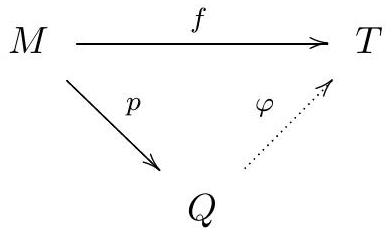
\includegraphics[max width=\textwidth, center]{2025_06_13_6ba93caed1e95a95104eg-092}\\
kommutiert.\\
Beweis. Wir zeigen zuerst die Eindeutigkeit bis auf eindeutigen Isomorphismus. Angenommen $p^{\prime}: M \rightarrow Q^{\prime}$ ist auch ein Quotientenmodul. Dann gilt $p^{\prime}\left(M^{\prime}\right)=0$ und somit gibt es eindeutig $\varphi: Q \rightarrow Q^{\prime}$ mit $p^{\prime}=\varphi \circ p$. Umgekehrt können wir genauso argumentieren und erhalten $\psi: Q^{\prime} \rightarrow Q$ mit $p=\psi \circ p^{\prime}$. Die Komposition $\psi \circ \varphi: Q \rightarrow Q$ erfüllt dann die geforderte Faktorisierungseigenschaft für $p: M \rightarrow Q$ bezüglich $p$. Da dies auch die Identität $\operatorname{id}_{Q}: Q \rightarrow Q$ erfüllt, folgt aus der Eindeutigkeit der Faktorisierung bereits $\psi \circ \varphi=\operatorname{id}_{Q}$. Umgekehrt schließt man genauso auf $\varphi \circ \psi=\operatorname{id}_{Q^{\prime}}$, so daß $\varphi$ und $\psi$ zueinander inverse $R$-Modulhomomorphismen sind. Außerdem sind diese eindeutig, wenn man Verträglichkeit mit den Quotientenabbildungen fordert. Das war rein formal!

Zur Existenz eines Quotientenmoduls überlegen wir uns nur, daß die Projektion

$$
p: M \rightarrow M / M^{\prime}
$$

ein Quotient ist. Das ist einfach: (1) Die Bedingung $p\left(M^{\prime}\right)=0$ folgt aus der Konstruktion sofort, und ein $f: M \rightarrow T$ mit $f\left(M^{\prime}\right)=0$ läßt die Definition von $\varphi: M / M^{\prime} \rightarrow T$ mittels

$$
\varphi\left(x+M^{\prime}\right):=f(x)
$$

zu. Dies ist wohldefiniert, da $f\left(M^{\prime}\right)=0$. Weiter ist $\varphi$ ein $R$-Modulhomomorphismus, wie man leicht durch Wahl geeigneter Vertreter und der Homomorphie von $f$ nachrechnet. Die Faktorisierungseigenschaft folgt sofort aus der Definition und ist gewissermaßen die Leitidee für die Definition. Auch die Eindeutigkeit ist offensichtlich.

Satz 11.28 (Homomorphiesatz). Sei $f: M \rightarrow N$ ein $R$-Modulhomomorphismus. Dann definiert

$$
\begin{aligned}
\varphi: M / \operatorname{ker}(f) & \rightarrow \operatorname{im}(f) \\
x+\operatorname{ker}(f) & \mapsto f(x)
\end{aligned}
$$

einen Isomorphismus von R-Moduln.\\
Beweis. Die Quotienteneigenschaft von $M \rightarrow M / \operatorname{ker}(f)$ nach Proposition 11.27 führt bezüglich $f: M \rightarrow N$ zu einem $R$-Modulhomomorphismus $M / \operatorname{ker}(f) \rightarrow N$, dessen Bild weiter $f(M)$ ist. Schränken wir das Ziel auf $\operatorname{im}(f)$ ein, so erhalten wir den behaupteten $R$-Modulhomomorphismus $\varphi$. Dieser ist offensichtlich surjektiv. Sei $x$ ein Vertreter im Urbild von $\bar{x} \in M / \operatorname{ker}(f)$. Dann ist $\varphi(\bar{x})=0$ genau dann, wenn $x \in \operatorname{ker}(f)$, also wenn $\bar{x}=0$. Damit ist $\varphi$ auch injektiv. Als bijektiver $R$-Modulhomomorphismus ist $\varphi$ ein Isomorphismus.

Bemerkung 11.29. Sei $M$ ein $R$-Modul und seien $M_{1}^{\prime}$ und $M_{2}^{\prime}$ Untermoduln von $M$.\\
(1) Schnitt $M_{1}^{\prime} \cap M_{2}^{\prime}$, und\\
(2) Summe $M_{1}^{\prime}+M_{2}^{\prime}=\left\{x_{1}+x_{2} ; x_{i} \in M_{i}^{\prime}\right.$ für $\left.i=1,2\right\}$\\
sind ebenfalls $R$-Untermoduln von $M$. Schnitt und Summe lassen sich auch für beliebige Familien indiziert durch eine Menge $A$ von Untermoduln $M_{\alpha}^{\prime} \subseteq M$ mit $\alpha \in A$ definieren.\\
Korollar 11.30 (Erster Isomorphiesatz). Sei $M$ ein $R$-Modul mit Untermoduln $K, L \subseteq M$. Dann induziert die Identität einen $R$-Modulisomorphismus

$$
K / K \cap L \xrightarrow{\sim} K+L / L
$$

Beweis. Das ist der Homomorphiesatz für Moduln angewandt auf $K \rightarrow M \rightarrow M / L$.\\
Korollar 11.31 (Zweiter Isomorphiesatz). Sei M ein R-Modul mit Untermoduln $K \subseteq L \subseteq M$. Dann induziert die Identität einen $R$-Modulisomorphismus

$$
(M / K) /(L / K) \xrightarrow{\sim} M / L .
$$

Beweis. Die Quotienteneigenschaft von $M \rightarrow M / K$ nach Proposition 11.27 führt bezüglich $M \rightarrow M / L$ zu einem $R$-Modulhomomorphismus $M / K \rightarrow M / L$. Der behauptete Isomorphismus folgt aus dem Homomorphiesatz angewandt auf $M / K \rightarrow M / L$.\\
11.4. Produkte und Summen von Moduln. Wir diskutieren nun Produkte und Summen für Moduln mit Blick auf ihre universelle Eigenschaft.

Definition 11.32. (1) Sei $M$ ein $R$-Modul und seien $M_{1}, \ldots, M_{s}$ Untermoduln. Man sagt $M$ ist die innere direkte Summe der $M_{i}$

$$
M=\bigoplus_{i=1}^{s} M_{i}
$$

wenn es für alle $x \in M$ eindeutige $x_{i} \in M_{i}$ für $i=1, \ldots, s$ gibt mit

$$
x=x_{1}+\ldots+x_{s}
$$

(2) Sei $I$ eine Menge und $N_{i}$ ein $R$-Modul für alle $i \in I$. Die direkte Summe von $R$-Moduln $N_{i}$ ist die Menge der Tupel

$$
\bigoplus_{i \in I} N_{i}=\left\{\left(x_{i}\right)_{i \in I} ; x_{i} \in N_{i} \text { für alle } i \in I \text { und } x_{i}=0 \text { für fast alle } i\right\}
$$

mit komponentenweiser Addition und $R$-Multiplikation. Bei endlicher Indexmenge $I$ ist die Bedingung leer, daß fast alle $x_{i}=0$ sind. Für $I=\{1, \ldots, s\}$ schreibt man auch $\bigoplus_{i=1}^{s} N_{i}$.\\
(3) Die (innere) direkte Summe von zwei $R$-Moduln $M$ und $N$ schreibt man auch $M \oplus N$.

Bemerkung 11.33. Sei $M$ die innere direkte Summe der Untermoduln $M_{i}$ für $i=1, \ldots, s$. Dann ist (mit der (abstrakten) direkten Summe) die Summenabbildung

$$
\bigoplus_{i=1}^{s} M_{i} \rightarrow M, \quad\left(x_{1}, \ldots, x_{s}\right) \mapsto \sum_{i=1}^{s} x_{i}
$$

Ein Isomorphismus von $R$-Moduln. Eine innere direkte Summe ist also isomorph zu einer (abstrakten) direkten Summe.

Beispiel 11.34. Für jedes $j \in I$ ist die Inklusion

$$
\iota_{j}: M_{j} \rightarrow \bigoplus_{i \in I} M_{i}
$$

mit $\iota_{j}(x)=(0, \ldots, x, \ldots, 0)$, wobei $x$ in der $j$-ten Koordinate sitzt, ein $R$-Modulhomomorphismus. Allgemeiner ist auch für eine Teilmenge $J \subseteq I$ die Inklusion

$$
\iota_{J}: \bigoplus_{j \in J} M_{j} \rightarrow \bigoplus_{i \in I} M_{i}
$$

mit der naheliegenden Definition der Fortsetzung eines Tupels durch 0 auf $I \backslash J$ ein $R$-Modulhomomorphismus.

Definition 11.35. Sei $R$ ein Ring. Das direkte Produkt einer Familie von $R$-Moduln $M_{i}$ für $i \in I$ ist der $R$-Modul

$$
\prod_{i \in I} M_{i}=\left\{\left(x_{i}\right)_{i \in I} ; x_{i} \in M_{i} \text { für alle } i \in I\right\}
$$

mit komponentenweiser Addition und $R$-Multiplikation. Für jedes $j \in I$ ist die Projektion

$$
\operatorname{pr}_{j}: \prod_{i \in I} M_{i} \rightarrow M_{j}
$$

mit $\operatorname{pr}_{j}\left(\left(x_{i}\right)\right)=x_{j}$ ein $R$-Modulhomomorphismus. Allgemeiner ist auch für eine Teilmenge $J \subseteq I$ die Projektion

$$
\operatorname{pr}_{J}: \prod_{i \in I} M_{i} \rightarrow \prod_{j \in J} M_{j}
$$

mit $\operatorname{pr}_{J}\left(\left(x_{i}\right)_{i \in I}\right)=\left(x_{j}\right)_{j \in J}$ ein $R$-Modulhomomorphismus.\\
Das Produkt zweier Moduln $M$ und $N$ schreiben wir als $M \times N$.\\
Satz 11.36 (Existenz von Produkten bei Moduln). Sei R ein Ring. Das direkte Produkt von RModuln $M_{i}$ mit $i \in I$ zusammen mit den Projektionen $\operatorname{pr}_{j}: \prod_{i \in I} M_{i} \rightarrow M_{j}$ erfüllt die universelle Eigenschaft des Produkts von $R$-Moduln:

Zu jedem $R$-Modul $T$ und $R$-Modulhomomorphismen $f_{i}: T \rightarrow M_{i}$ für alle $i \in I$ gibt es genau einen $R$-Modulhomomorphismus $f: T \rightarrow \prod_{i \in I} M_{i}$ mit $f_{i}=\operatorname{pr}_{i} \circ f$ für alle $i \in I$.

Beweis. Übung. Wie bei Ringen.

Satz 11.37 (Existenz von Summen bei Moduln). Sei R ein Ring. Die direkte Summe von RModuln $M_{i}$ mit $i \in I$ zusammen mit den Inklusionen $\iota_{j}: M_{j} \rightarrow \bigoplus_{i \in I} M_{i}$ erfüllt die universelle Eigenschaft der Summe von $R$-Moduln:

Zu jedem $R$-Modul $T$ und $R$-Modulhomomorphismen $f_{i}: M_{i} \rightarrow T$ für alle $i \in I$ gibt es genau einen $R$-Modulhomomorphismus $f: \bigoplus_{i \in I} M_{i} \rightarrow T$ mit $f_{i}=f \circ \iota_{i}$ für alle $i \in I$.

Beweis. Übung: $f\left(\left(x_{i}\right)_{i \in I}\right)=\sum_{i} f_{i}\left(x_{i}\right)$ definiert $f$, denn die Summe ist endlich.

\subsection*{Annulatorideale, zyklische Moduln.}
Definition 11.38. Sei $M$ ein $R$ Modul.\\
(1) Das Annulatorideal von $x \in M$ ist das Ideal

$$
\operatorname{Ann}_{R}(x)=\{a \in R \mid a x=0\} .
$$

(2) Das Annulatorideal von $M$ ist

$$
\operatorname{Ann}_{R}(M)=\{a \in R \mid \text { für alle } x \in M: a x=0\}=\bigcap_{x \in M} \operatorname{Ann}_{R}(x) .
$$

Es ist eine einfache Übung nachzurechnen, daß ein Annulatorideal wirklich ein Ideal ist. Zum Beispiel ist

$$
\operatorname{Ann}_{R}(x)=\operatorname{ker}(R \rightarrow M, \quad a \mapsto a x),
$$

und $\operatorname{Ann}_{R}(M)$ ist ein Ideal als Schnitt von Idealen.\\
Beispiel 11.39. (1) Es gilt $\operatorname{Ann}_{R}(R / I)=I$, denn $R / I$ wird von der Restklasse 1 modulo $I$ erzeugt, und es gilt $a \cdot 1=0 \in R / I$ genau dann, wenn $a \in I$.\\
(2) Wenn $M=\left\langle x_{1}, \ldots, x_{n}\right\rangle_{R}$, dann ist

$$
\operatorname{Ann}_{R}(M)=\left\{a \in R ; a x_{i}=0 \text { für alle } i=1, \ldots, n\right\}=\bigcap_{i=1}^{n} \operatorname{Ann}_{R}\left(x_{i}\right),
$$

weil ein $a$, das alle $x_{i}$ annuliert, auch alle $R$-Linearkombinationen der $x_{i}$ annuliert.\\
Definition 11.40. Ein zyklischer $R$-Modul ist ein $R$-Modul $M$, der von einem Element $x \in M$ erzeugt wird. Wir schreiben $M=\langle x\rangle_{R}=: R x$.

Proposition 11.41. Sei $R x=\langle x\rangle_{R} \subseteq M$ der zyklische R-Untermodul mit Erzeuger $x \in M$. Dann ist

$$
R / \operatorname{Ann}_{R}(x) \xrightarrow{\sim} R x, \quad[a] \mapsto a x
$$

ein R-Modulisomorphismus.\\
Beweis. Zu $x \in M$ gehört der $R$-Modulhomomorphismus $\cdot x: R \rightarrow M$ definiert durch $a \mapsto a x$. Der Annulator von $x$ ist

$$
\operatorname{Ann}_{R}(x)=\operatorname{ker}(\cdot x: R \rightarrow M) .
$$

Das Bild von $\cdot x: R \rightarrow M$ ist der von $x$ erzeugte $R$-Untermodul $\langle x\rangle_{R}=R x$. Die Behauptung folgt nun sofort aus dem Homomorphiesatz, Satz 11.28.

Beispiel 11.42. Sei $R=\mathbb{Z}$. Ein zyklischer $\mathbb{Z}$-Modul ist eine abelsche Gruppe, die von einem Element erzeugt wird. Das ist also nichts anderes als eine zyklische Gruppe, somit isomorph zu $\mathbb{Z}$ oder zu $\mathbb{Z} / n \mathbb{Z}$ für ein $n \geq 1$.

Wir können nun den Satz über die Existenz der Jordannormalform nach Proposition 11.10 in der Sprache der Moduln formulieren.

Proposition 11.43. Sei $K$ ein Körper. Um die Existenz der Jordannormalform zu beweisen, reicht die folgenden Aussage:

Sei $V$ ein $K[X]$-Modul, der als $K$-Vektorraum endlich-dimensional ist. Dann ist $V$ eine endliche direkte Summe von zyklischen $K[X]$-Moduln.

Beweis. Ein solcher zyklischer $K[X]$-Modul hat nach Proposition 11.41 die Form $K[X] / I$ für ein Ideal $I$. Weil $K[X]$ ein Hauptidealring ist, muß $I=(P)$ sein für ein Polynom $P \in K[X]$. Dabei kann $P=0$ nicht auftreten, weil sonst $V$ einen $K$-Unterraum isomorph zu $K[X]$ enthielte, was der endlichen Dimension von $V$ widerspräche.

Um die Existenz der Jordannormalform aus Proposition 11.10 zu bekommen, müssen wir aus einer Zerlegung in Summanden $K[X] /(P)$ eine Zerlegung in solche zyklische $K[X]$-Moduln machen, bei denen $P$ eine Potenz eines Primpolynoms ist. Wir zerlegen einfach die Sumannden weiter nach dem Chinesischen Restsatz, Korollar 10.17. Denn wenn $P$ die Zerlegung $\prod_{i=1}^{s} P_{i}^{r_{i}}$ hat, dann ist als Ringe

$$
K[X] /(P) \simeq \prod_{i=1}^{s} K[X] /\left(P_{i}^{r_{i}}\right)
$$

und man überzeugt sich sofort, daß der Ringisomorphismus, der im Beweis des Chinesischen Restsatzes angegeben wurde, auch ein $K[X]$-Modulisomorphismus ist.

\section*{Übungsaufgaben zu §11}
Übungsaufgabe 11.1. Zeigen Sie, daß ein direkter Summand eines endlich erzeugten $R$-Moduls selbst endlich erzeugt ist, d.h. ist $M \simeq \bigoplus_{i=1}^{s} M_{i}$, und $M$ ist endlich erzeugt, dann sind auch die $M_{i}$ endlich erzeugt.

\section*{Moduln Über Hauptidealringen}
12.1. Torsion. In diesem Abschnitt sei zur Vereinfachung $R$ ein Integritätsring. Für den allgemeinen Fall haben wir die Bedingung ,, $a \neq 0$ " durch ,, $a$ ist kein Nullteiler" zu ersetzen.

Bemerkung 12.1. Sei $M$ ein $R$-Modul, und sei $a \in R$. Die Abbildung $x \mapsto a x$, also die Multiplikation mit $a$, definiert einen $R$-Modulhomomorphismus

$$
[a]: M \rightarrow M, \quad[a](x)=a x
$$

Der Kern $M[a]:=\operatorname{ker}([a]: M \rightarrow M)$ ist damit offensichtlich ein $R$-Untermodul von $M$.\\
Definition 12.2. Sei $R$ ein Integritätsring, und sei $M$ ein $R$-Modul.\\
(1) Ein $x \in M$ ist ein Torsionselement, wenn es ein $0 \neq a \in R$ gibt mit $a x=0$.\\
(2) Sei $a \in R, a \neq 0$. Wir bezeichnen den Kern $M[a]=\operatorname{ker}([a])$ der Multiplikation mit $a$, also

$$
M[a]=\{x \in M ; a x=0\}
$$

als den $R$-Untermodul der $a$-Torsion(selemente) von $M$.\\
(3) Der Modul $M$ ist ein Torsionsmodul, wenn jedes $x \in M, x \neq 0$ ein Torsionselement ist.

Bemerkung 12.3. Sei $M$ ein $R$-Modul. Sind $a, b \in R$ assoziiert, d.h. es gibt eine Einheit $\varepsilon \in R^{\times}$ mit $a=\varepsilon b$, dann ist für alle $x \in M$

$$
a x=0 \Longleftrightarrow b x=0
$$

weil man mit $\varepsilon$ bzw. $\varepsilon^{-1}$ multiplizieren kann. Daher ist dann

$$
M[a]=M[b]
$$

Beispiel 12.4. Sei $R=K[X]$ ein Polynomring über einem Körper $K$. Sei $V$ ein endlichdimensionaler $K$-Vektorraum mit Endomorphismus $\varphi: V \rightarrow V$, den wir durch $X v=\varphi(v)$ für alle $v \in V$ als $K[X]$-Modul auffassen.\\
(1) Bezüglich des Polynoms $X-\lambda$ gilt: die $(X-\lambda)$-Torsion

$$
V[X-\lambda]=V_{\lambda}
$$

ist der Eigenraum von $\varphi$ zum Eigenwert $\lambda$.\\
(2) Für $r \geq 1$ und $\lambda \in K$ bezeichnen wir als verallgemeinerten Eigenraum (der Stufe $r$ ) den Unterraum

$$
V_{\lambda, r}:=V\left[(X-\lambda)^{r}\right] .
$$

Die verallgemeinerten Eigenräume bilden eine bezüglich Inklusion aufsteigende Folge von $K$-Untervektorräumen von $V$ :

$$
\{0\}=V_{\lambda, 0} \subseteq V_{\lambda}=V_{\lambda, 1} \subseteq V_{\lambda, 2} \subseteq \ldots \subseteq V_{\lambda, r} \subseteq \ldots,
$$

deren Vereinigung der verallgemeinerten Eigenraum von $\varphi$ zum Eigenwert $\lambda$ ist.\\
(3) Sei $m_{\varphi}(X)$ das Minimalpolynom von $\varphi$. Dann ist $V$ ein Torsionsmodul, denn es gilt

$$
V=V\left[m_{\varphi}(X)\right]
$$

Proposition 12.5. Sei $R$ ein Integritätsring, und sei $M$ ein endlich erzeugter $R$-Modul. Dann ist $M$ ein Torsionsmodul genau dann, wenn es $0 \neq a \in R$ gibt mit $M=M[a]$.

Beweis. Wenn für ein $0 \neq a \in R$ gilt $M=M[a]$, dann sind alle $x \in M$ Torsionselemente, nämlich $a$-Torsion. Daher ist $M$ ein Torsionsmodul.

Sei umgekehrt $M$ ein Torsionsmodul und von den Elementen $x_{1}, \ldots, x_{n}$ erzeugt als $R$-Modul. Weil $M$ Torsion ist, gibt es $a_{1}, \ldots, a_{n}$ verschieden von 0 mit $a_{i} x_{i}=0$ für alle $i=1, \ldots, n$. Dann ist $a=a_{1} \cdot \ldots \cdot a_{n}$ ebenfalls nicht 0 , denn $R$ ist ein Integritätsring. Weiter gilt für alle $i=1, \ldots, n$

$$
a x_{i}=\left(a_{1} \cdot \ldots a_{i-1} \cdot a_{i+1} \cdot a_{n}\right) \cdot\left(a_{i} x_{i}\right)=\left(a_{1} \cdot \ldots a_{i-1} \cdot a_{i+1} \cdot a_{n}\right) \cdot 0=0
$$

Damit gilt $x_{i} \in M[a]$ für alle $i=1, \ldots, n$. Weil $M$ von den Elementen $x_{i}$ erzeugt wird, folgt

$$
\left.M=\left\langle x_{1}, \ldots, x_{n}\right\rangle\right)_{R} \subseteq M[a] \subseteq M
$$

also $M=M[a]$.\\
12.2. Die Primärzerlegung von Torsionsmoduln. Ab jetzt bis zum Ende des Kapitels ist $R$ ein Hauptidealring. Wir denken speziell an die Fälle $K[X]$ und $\mathbb{Z}$.

Definition 12.6. Sei $R$ ein Hauptidealring, sei $M$ ein $R$-Modul und sei $p \in R$ ein Primelement. Die Elemente von $M$, welche von einer Potenz von $p$ annulliert werden, nennt man $p$-primär. Die $p$-primären Elemente von $M$ bilden den Untermodul, eine Vereinigung

$$
M\left[p^{\infty}\right]:=\bigcup_{r \geq 0} M\left[p^{r}\right]
$$

einer aufsteigenden Kette von Untermoduln

$$
\{0\}=M\left[p^{0}\right] \subseteq M[p] \subseteq M\left[p^{2}\right] \subseteq \ldots \subseteq M\left[p^{r}\right] \subseteq M\left[p^{r+1}\right] \subseteq \ldots
$$

Der Untermodul $M\left[p^{\infty}\right]$ wird die $p$-primäre Komponente von $M$ genennt. Gilt $M=M\left[p^{\infty}\right]$, so nennt man $M p$-primär.

Der folgende Satz verallgemeinert die Eigenraumzerlegung eines diagonalisierbaren Endomorphimus. Hier hat überdies der Chinesische Restsatz seinen prominenten Auftritt.

Satz 12.7 (Primärzerlegung). Seien $R$ ein Hauptidealring und $M$ ein endlich erzeugter Torsionsmodul. Dann gilt:\\
(1) $M$ ist direkte Summe seiner p-Primärkomponenten:

$$
M=\bigoplus_{p \text { prim }} M\left[p^{\infty}\right]
$$

wobei $p$ durch ein Vertretersystem der Äquivalenzklassen von Primelementen von $R$ bis auf Assoziiertheit läuft.\\
(2) Für alle Primelemente $p \in R$ ist $M\left[p^{\infty}\right]$ ein endlich erzeugter $R$-Modul und für fast alle Klassen von Primelementen bis auf Assoziiertheit gilt $M\left[p^{\infty}\right]=0$.\\
(3) Sei $0 \neq a \in R$ mit $M=M[a]$, und sei $a=u \cdot \prod_{i=1}^{s} p_{i}^{\alpha_{i}}$ seine Zerlegung in Primfaktoren, und $u \in R^{\times}$. Dann ist $M\left[p_{i}^{\infty}\right]=M\left[p_{i}^{\alpha_{i}}\right]$ für $i=1, \ldots, s$ ein endlich erzeugter $R$-Modul, und es gilt genauer

$$
M=\bigoplus_{i=1}^{s} M\left[p_{i}^{\alpha_{i}}\right]
$$

Beweis. Wir zeigen zuerst die Behauptung (3), dann (2), und Aussage (1) folgt dann mittels Proposition 12.5.

Schritt 0: Modulo (a). Als Vorüberlegung betrachten wir $b, c \in R$ und folgern aus einer Kongruenz $b \equiv c(\bmod (a))$, also wenn $[b]=[c]$ in $R /(a)$ gilt, daß dann die $R$-Multiplikation des Moduls mit einem beliebigen $x \in M$ gleich ausfällt: $b x=c x$. In der Tat gilt dann $c-b=\Delta \in(a)$, so daß

$$
c x=(b+\Delta) x=b x+\Delta x=b x
$$

denn $\Delta \in(a) \subseteq \operatorname{Ann}_{R}(M)$.\\
Schritt 1: Projektoren. Nach dem Chinesischen Restsatz, genauer Korollar 10.17, haben wir einen natürlichen Ringisomorphismus

$$
R /(a) \simeq \prod_{i=1}^{s} R /\left(p_{i}^{\alpha_{i}}\right)
$$

Sei $e_{i} \in R$ ein Element, das im Produkt geht auf $(0, \ldots, 1, \ldots, 0)$ mit der einzigen 1 an der $i$-ten Position. Dann gilt für alle $i, j$ modulo ( $a$ )

$$
\begin{aligned}
e_{i} e_{j} & \equiv \delta_{i, j} e_{i} \\
\sum_{i=1}^{s} e_{i} & \equiv 1
\end{aligned}
$$

Weil $(a) \subseteq \operatorname{Ann}_{R}(M)$, folgt für alle $x \in M$

$$
\begin{aligned}
e_{i} e_{j} x & =\delta_{i, j} e_{j} x \\
\left(\sum_{i=1}^{s} e_{i}\right) x & =x
\end{aligned}
$$

Schritt 2: Direkte Summe. Mit den Untermoduln $e_{i} M=\left\{e_{i} x \mid x \in M\right\}$ von $M$ definieren wir zwei $R$-Modulhomomorphismen

$$
\begin{aligned}
& S: \bigoplus_{i=1}^{n} e_{i} M \rightarrow M, \quad S\left(x_{1}, \ldots, x_{n}\right)=\sum_{i=1}^{s} x_{i} \\
& E: M \rightarrow \bigoplus_{i=1}^{n} e_{i} M, \quad E(x)=\left(e_{1} x, \ldots, e_{n} x\right)
\end{aligned}
$$

Es sind $S$ und $E$ zueinander inverse Isomorphismen, denn zuerst einmal gilt

$$
S(E(x))=\sum_{i=1}^{s} e_{i} x=\left(\sum_{i=1}^{s} e_{i}\right) x=x
$$

Sodann gibt es für $x=\left(x_{1}, \ldots, x_{n}\right) \in \bigoplus_{i=1}^{n} e_{i} M$ für $j=1, \ldots, s$ Elemente $y_{j} \in M$ mit $x_{j}=e_{j} y_{j}$, so daß

$$
\begin{aligned}
E(S(x)) & =E\left(S\left(x_{1}, \ldots, x_{n}\right)\right)=E\left(\sum_{j=1}^{s} e_{j} y_{j}\right) \\
& =\left(e_{i} \sum_{j=1}^{s} e_{j} y_{j}\right)_{1 \leq i \leq s}=\left(\sum_{j=1}^{s} \delta_{i, j} e_{j} y_{j}\right)_{1 \leq i \leq s}=\left(x_{1}, \ldots, x_{n}\right)=x
\end{aligned}
$$

Damit haben wir gezeigt:

$$
M=\bigoplus_{i=1}^{s} e_{i} M
$$

Schritt 3: Endlich erzeugt. Der direkte Summand $e_{i} M$ ist das Bild des $R$-Modulhomomorphismus $e_{i} \cdot: M \rightarrow M$. Weil $M$ endlich erzeugt ist, ist damit das Bild $e_{i} M$ ebenfalls endlich erzeugt.

Schritt 4: Identifikation der Summanden. Wir haben nun $e_{i} M=M\left[p_{i}^{\alpha_{i}}\right]=M\left[p_{i}^{\infty}\right]$ nachzuweisen. Wieder gilt modulo (a)

$$
p_{i}^{\alpha_{i}} e_{i} \equiv 0, \quad \text { also } \quad p_{i}^{\alpha_{i}} e_{i} \in(a)
$$

Weil $(a) \subseteq \operatorname{Ann}_{R}(M)$ gilt nach Voraussetzung, folgt für alle $x \in M$

$$
p_{i}^{\alpha_{i}} e_{i} x=0
$$

Das bedeutet

$$
e_{i} M \subseteq M\left[p_{i}^{\alpha_{i}}\right] \subseteq M\left[p_{i}^{\infty}\right]
$$

Sei nun $x \in M\left[p_{i}^{\infty}\right]$ beliebig. Dann gibt es $\beta \geq 1$ mit $p_{i}^{\beta} x=0$. Per Konstruktion ist $e_{i} \equiv 1$ modulo $p_{i}^{\alpha_{i}}$. Damit gibt es $z_{i} \in R$ mit

$$
e_{i}=1+z_{i} p_{i}^{\alpha_{i}}
$$

woraus

$$
1 \in\left(e_{i}, p_{i}^{\alpha_{i}}\right) \subseteq\left(e_{i}, p_{i}\right)
$$

folgt. Damit ist $e_{i}$ teilerfremd zu $p_{i}$. Aufgrund der eindeutigen Primfaktorzerlegung in $R$ nach Theorem 9.23 ist dann auch $e_{i}$ teilerfremd zu $p_{i}^{\beta}$. Das Lemma von Bezout, Korollar 10.7, gibt Elemente $b_{i}, c_{i} \in R$ mit

$$
1=b_{i} e_{i}+c_{i} p_{i}^{\beta}
$$

Damit folgt

$$
x=\left(b_{i} e_{i}+c_{i} p_{i}^{\beta}\right) x=e_{i}\left(b_{i} x\right)+c_{i}\left(p_{i}^{\beta} x\right)=e_{i}\left(b_{i} x\right) \in e_{i} M
$$

Dies zeigt

$$
M\left[p_{i}^{\infty}\right] \subseteq e_{i} M
$$

und zusammen mit (12.1) folgt die behauptete Gleichheit

$$
e_{i} M=M\left[p_{i}^{\alpha_{i}}\right]=M\left[p_{i}^{\infty}\right]
$$

Schritt 5: Die anderen Primärkomponenten. Sei $p$ ein Primelement, das teilerfremd zu $a$ ist, also nicht zu einem der $p_{1}, \ldots, p_{s}$ assoziiert ist. Sei $x \in M\left[p^{\infty}\right]$, etwa mit $p^{\beta} x=0$ für ein $\beta \geq 1$. Das Lemma von Bezout, Korollar 10.7, gibt Elemente $b, c \in R$ mit

$$
1=b a+c p^{\beta}
$$

Damit folgt

$$
x=\left(b a+c p^{\beta}\right) x=b(a x)+c\left(p^{\beta} x\right)=0
$$

weil $x \in M=M[a]$. Dies zeigt $M\left[p^{\infty}\right]=0$.\\
Bemerkung 12.8. Mit der Notation aus Satz 12.7 gilt $a \in \operatorname{Ann}_{R}(M)$. Da $R$ ein Hauptidealring ist, gibt es ein bezüglich Teilbarkeit kleinstes a mit dieser Eigenschaft, nämlich dann, wenn $\operatorname{Ann}_{R}(M)=(a)$ ist.

Korollar 12.9 (Kernzerlegung). Sei $V$ ein endlich-dimensionaler $K$-Vektorraum mit einem Endomorphismus $\varphi$. Sei $\chi_{\varphi}(X)=\prod_{i=1}^{s} p_{i}(X)^{\alpha_{i}}$ die Primfaktorzerlegung des charakteristischen Polynoms in $K[X]$. Dann gilt:\\
(1) $\quad V=\bigoplus_{i=1}^{s} V_{p_{i}}$ mit den verallgemeinerten Eigenräumen $V_{p_{i}}=\operatorname{ker}\left(p_{i}(\varphi)^{\alpha_{i}}\right) \subseteq V$.\\
(2) Die Projektoren $E_{i}: V \rightarrow V_{p_{i}} \subseteq V$ der Zerlegung als direkte Summe in (1) sind gegeben durch Polynome in $\varphi$. Insbesondere kommutieren die Projektoren mit allen Endomorphismen von $V$, die mit $\varphi$ vertauschen, die deshalb auch die Zerlegung $V=\bigoplus_{i=1}^{s} V_{p_{i}}$ respektieren.

Beweis. Wir fassen wie üblich $V$ als $K[X]$-Modul auf, indem wir $X$ durch $\varphi$ operieren lassen. Eine $K$-Basis von $V$ erzeugt $V$ erst recht auch als $K[X]$-Modul. Damit ist $V$ ein endlich erzeugter $K[X]$-Modul. Nach dem Satz von Cayley-Hamilton gilt $\chi_{\varphi}(\varphi)=0$, also

$$
\chi_{\varphi}(X) \in \operatorname{Ann}_{K[X]}(V)
$$

Damit folgt das Korollar sofort aus Satz 12.7. Die Projektoren $e_{i}$ im Beweis von Satz 12.7 sind nun Polynome $e_{i}(X) \in K[X]$, und deren Effekt auf $V$ wird gegeben durch $E_{i}=e_{i}(\varphi)$.

Kommutiert ein $\psi: V \rightarrow V$ mit $\varphi$, dann gilt für alle Polynome $P(X)=\sum_{i=0}^{d} a_{i} X^{i}$

$$
\psi \circ(P(\varphi))=\psi \circ\left(a_{0}+a_{1} \varphi+\ldots+a_{d} \varphi^{d}\right)=\left(a_{0}+a_{1} \varphi+\ldots+a_{d} \varphi^{d}\right) \circ \psi=(P(\varphi)) \circ \psi .
$$

Insbesondere gilt dann $\psi \circ E_{i}=E_{i} \circ \psi$, so daß $\psi$ das Bild von $E_{i}$ in sich abbildet. Damit ist die Zerlegung $V=\bigoplus_{i=1}^{s} V_{p_{i}}$ eine Zerlegung in $\psi$-stabile Unterräume.\\
Korollar 12.10. Seien $R$ ein Hauptidealring, $p$ ein Primelement und $M$ ein endlich erzeugter Torsionsmodul. Dann ist die p-primäre Komponente $M\left[p^{\infty}\right]$ ein endlich erzeugter Torsionsmodul.

Beweis. In der Notation des Beweises zu Satz 12.7 ohne den index $i$, haben wir $e \in R$ und $\alpha \in \mathbb{N}$ mit $M\left[p^{\infty}\right]=e M=M\left[p^{\alpha}\right]$. Als $e M$ ist die $p$-primäre Komponente das Bild des $R$ Modulhomomorphismu $[e]: M \rightarrow M$, der Multiiplikation mit $e$. Als Bild eines endlich erzeugten $R$-Moduls ist $e M$ auch endlich erzeugt.

Die $p$-primäre Komponente besteht nur aus $p$-Potenz-Torsion, ist also insbesondere ein Torsionsmodul.\\
12.3. Die Struktur von Torsionsmoduln. In diesem Kapitel beweisen wir den folgenden Struktursatz.

Satz 12.11 (Struktursatz für endlich erzeugte Torsionsmoduln). Sei $R$ ein Haupidealring und $M$ ein endlich erzeugter Torsionsmodul. Dann gilt:\\
(1) $M$ ist isomorph zu einer direkten Summe zyklischer Moduln.\\
(2) Es gibt nicht notwendig verschiedene Primelemente $p_{i}, i=1, \ldots, s$ und natürliche Zahlen $\alpha_{i}, i=1, \ldots, s$, so daß

$$
M \cong \bigoplus_{i=1}^{s} R /\left(p_{i}^{\alpha_{i}}\right)
$$

Beweis. Offenbar ist (1) eine Folge der präziseren Strukturaussage (2). Um (2) zu beweisen, dürfen wir nach der Primärzerlegung, Satz 12.7, den Modul $M$ durch seine $p$-Primärkomponente $M\left[p^{\infty}\right]$ zu einem Primelement $p$ ersetzen. Die $p$-Primärkomponente erbt die Voraussetzung, endlich erzeugter Torsionsmodul zu sein, nach Korollar 12.10 von $M$.

Weil die $p$-Primärkomponente endlich erzeugt ist, reicht nach Proposition 12.5 bereits eine uniformen Potenz $p^{e}$, um alle Elemente zu annulieren. Es gibt also eni $e$ mit $\left(p^{e}\right) \subseteq \operatorname{Ann}_{R}(M)$. Weil $R$ ein Hauptidealring ist, gilt $\operatorname{Ann}_{R}(M)=(a)$ für ein $a \in R$ und $a \mid p^{e}$. Aufgrund der eindeutigen Primfaktorzerlegung, Theorem 9.23, ist daher der Annulator ebenfalls von einer Potenz von $p$ erzeugt.

Sei also nun oBdA $\operatorname{Ann}_{R}(M)=\left(p^{e}\right)$. Für alle $x \in M$ ist dann $\left(p^{e}\right) \subseteq \operatorname{Ann}_{R}(x)$ und daher mit dem selben Argument wie eben $\operatorname{Ann}_{R}(x)=\left(p^{\alpha}\right)$ für ein geeignetes $p^{\alpha} \mid p^{e}$, also ein $\alpha \leq e$. Es\\
reicht nun eine direkte Zerlegung $M=\bigoplus_{i} R x_{i}$ mit endlich vielen Elementen $x_{i} \in M$ zu finden, denn dann ist $\operatorname{Ann}_{R}\left(x_{i}\right)=\left(p^{\alpha_{i}}\right)$ für geeignete $\alpha_{i} \leq e$, und nach Proposition 11.41 folgt

$$
M=\bigoplus_{i=1}^{s} R x_{i}=\bigoplus_{i=1}^{s} R /\left(p_{i}^{\alpha_{i}}\right)
$$

Wir führen nun Induktion über die Anzahl $n$ einer Erzeugermenge von $M$. Der Induktionsanfang $n=0$ mit einer leeren Erzeugermenge führt zum Modul $M=0$, der die leere direkte Summe zyklischer Moduln ist. (Wem das suspekt ist, der analysiere den Fall mit nur einem Erzeuger.)

Behandeln wir nun den Induktionsschritt. Es besitze $M$ ein Erzeugendensystem aus $n$ Elementen $z_{1}, z_{2}, \ldots z_{n}$. Unter diesen gibt es ein Element, oE $x_{1}:=z_{1}, \operatorname{mit} \operatorname{Ann}_{R}\left(x_{1}\right)=\left(p^{e}\right)$ und $e$ maximal, denn sonst annulierte schon $p^{e-1}$ den Modul $M$, siehe den Beweis von Proposition 12.5.

Der Quotient pr : $M \rightarrow \bar{M}=M / R x_{1}$ kann mit den $n-1$ Bildern $\bar{z}_{i}=\operatorname{pr}\left(z_{i}\right)$ erzeugt werden. Per Induktionsvoraussetzung gibt es $\bar{y}_{2}, \ldots, \bar{y}_{s} \in \bar{M}$ mit

$$
\bar{M}=\bigoplus_{i=2}^{s} R \bar{y}_{i}
$$

Wir werden versuchen diese Zerlegung nach $M$ zu liften. Dazu liften wir zunächst die $\bar{y}_{i}$ beliebig zu $y_{i} \in M$ mit $\operatorname{pr}\left(y_{i}\right)=\bar{y}_{i}$. Sei $\operatorname{Ann}_{R}\left(\bar{y}_{i}\right)=\left(p^{e_{i}}\right)$. Dann gilt $e_{i} \leq e$ und $p^{e_{i}} y_{i} \in \operatorname{ker}(\operatorname{pr})=R x_{1}$. Es gibt also $a_{i} \in R$ mit

$$
p^{e_{i}} y_{i}=a_{i} x_{1}
$$

Jetzt verwenden wir die Extremalität von $x_{1}$. Da $p^{e-e_{i}} a_{i} x_{1}=p^{e} y_{i}=0$ muß $p^{e_{i}}$ ein Teiler von $a_{i}$ sein. Wir setzen $a_{i}=p^{e_{i}} b_{i}$ und modifizieren $y_{i}$ ohne sein Bild in $\bar{M}$ zu ändern durch $x_{i}=y_{i}-b_{i} x_{1}$. Damit annulliert $p^{e_{i}}$ den Lift $x_{i}$ wegen

$$
p^{e_{i}} x_{i}=p^{e_{i}}\left(y_{i}-b_{i} x_{1}\right)=p^{e_{i}} y_{i}-p^{e_{i}} b_{i} x_{1}=p^{e_{i}} y_{i}-a_{i} x_{1}=0
$$

Wir zeigen nun, daß $M$ die direkte Summe der $R x_{i}$ ist. Sei $x \in M$ beliebig. Dann gibt es $a_{2}, \ldots, a_{s} \in R$ mit $\operatorname{pr}(x)=\sum_{i=2}^{s} a_{i} \bar{y}_{i}$. Dann ist

$$
\operatorname{pr}\left(x-\sum_{i=2}^{s} a_{i} x_{i}\right)=\operatorname{pr}(x)-\sum_{i=2}^{s} a_{i} \operatorname{pr}\left(x_{i}\right)=\operatorname{pr}(x)-\sum_{i=2}^{s} a_{i} \bar{y}_{i}=0
$$

Damit ist $x-\sum_{i=2}^{s} a_{i} x_{i} \in \operatorname{ker}(\mathrm{pr})=R x_{1}$, und damit wird $M$ von den $x_{1}, \ldots, x_{s}$ erzeugt. Es bleibt zu zeigen, daß die Summe der $R x_{i}$ direkt ist, d.h. die Summenabbildung

$$
\bigoplus_{i=1}^{s} R x_{i} \rightarrow M
$$

ist eine $R$-Modulisomorphismus.\\
Sei $a_{i} x_{i} \in R x_{i}$ mit $\sum_{i=1}^{s} a_{i} x_{i}=0$. Dann ist $0=\operatorname{pr}\left(\sum_{i=1}^{s} a_{i} x_{i}\right)=\sum_{i=2}^{s} a_{i} \bar{y}_{i}$. Weil $\bar{M}$ die direkte Summe der $R \bar{y}_{i}$ ist, folgt $a_{i} \bar{y}_{i}=0$. Weil $\operatorname{Ann}_{R}\left(x_{i}\right)=\left(p^{e_{i}}\right)=\operatorname{Ann}_{R}\left(\bar{y}_{i}\right)$ für alle $i=2, \ldots, s$ gilt, folgt auch $a_{i} x_{i}=0$. Und schließlich folgt damit $a_{1} x_{1}=\sum_{i=1}^{s} a_{i} x_{i}=0$. Damit sind alle Komponenten in den $R x_{i}$ Null, wenn ihre Summe 0 ergibt: die Summe der Untermoduln ist eine direkte Summe.

Wir kommen nun zur Jordannormalform zurück.\\
Beweis. Wir beweisen nun die Existenz der Jordannormalform aus Theorem 11.7 (1) für einen Endomorphismus $\varphi: V \rightarrow V$ eines endlich-dimensionalen $K$-Vektorraums. Dazu bedienen wir uns der Übersetzung in die Sprache der $K[X]$-Moduln aus Proposition 11.10. Diese modultheoretische Aussage ist nichts anderes als der Struktursatz Satz 12.11 für den Hauptidealring $R=K[X]$, sofern wir einsehen, daß durch die Interpretation als $K[X]$-Modul aus dem Vektorraum $V$ ein endlich erzeugter Torsionsmodul wird. Letzteres haben wir uns zu Beginn des Beweises von Korollar 12.9 überlegt.

Wir bezeichnen zu einem Primelement $p$ eines Hauptidealrings $R$ den Restklassenring $R /(p)$ mit $\kappa(p)$. Der Ring $\kappa(p)$ ist nach Proposition 9.12 ein Körper. Sei $M$ ein $R$-Modul. Die $R$ Modulstruktur auf den Quotienten $M\left[p^{\alpha}\right] / M\left[p^{\alpha-1}\right]$ ist wohldefiniert modulo ( $p$ ), weil

$$
p M\left[p^{\alpha}\right] \subseteq M\left[p^{\alpha-1}\right] .
$$

Daher ist $M\left[p^{\alpha}\right] / M\left[p^{\alpha-1}\right]$ auf natürliche Weise durch die Multiplikation mit Repräsentanten ein $\kappa(p)$-Vektorraum.

Satz 12.12 (Eindeutigkeit). Sei $R$ ein Hauptidealring, und sei $M$ ein endlich erzeugter Torsionsmodul mit einer Zerlegung

$$
M \simeq \bigoplus_{i=1}^{s} R /\left(p_{i}^{\alpha_{i}}\right)
$$

wie in Satz 12.11. Sei $p$ ein Primelement von $R$, und sei $\beta \geq 1$. Dann gilt:\\
(1) Die Anzahl der p-primären zyklischen Summanden ist

$$
\#\left\{i ; p_{i} \sim p \text { assoziiert }\right\}=\operatorname{dim}_{\kappa(p)}(M / p M)=\operatorname{dim}_{\kappa(p)}(M[p])
$$

(2) Die Anzahl der p-primären zyklischen Summanden mit Exponent $\beta$ ist

$$
\#\left\{i ; p_{i} \sim p \text { assoziiert, und } \alpha_{i}=\beta\right\}=\operatorname{dim}_{\kappa(p)}\left(M\left[p^{\beta}\right] / M\left[p^{\beta-1}\right]\right)-\operatorname{dim}_{\kappa(p)}\left(M\left[p^{\beta+1}\right] / M\left[p^{\beta}\right]\right)
$$

Insbesondere sind die Anzahl der Summanden und genauer die Anzahl der Summanden mit Annulator ( $p^{\beta}$ ) unabhängig von der gewählten Zerlegung.\\
Beweis. Aus $M=M^{\prime} \oplus M^{\prime \prime}$ folgt $p M=p M^{\prime} \oplus p M^{\prime \prime}$ und $M\left[p^{\beta}\right]=M^{\prime}\left[p^{\beta}\right] \oplus M^{\prime \prime}\left[p^{\beta}\right]$. Da Quotienten nehmen mit direkten Summen verträglich ist, und die Dimension eines Vektorraums additiv auf direkten Summen ist, gelten die Formeln in (1) und (2) für $M$ genau dann, wenn sie für $M^{\prime}$ und $M^{\prime \prime}$ gelten. Wir haben also nur den Fall $M=R /\left(p^{\beta}\right)$ mit $\beta>0$ zu analysieren (das entspricht einem einzelnen Jordankästchen). Diesen Fall überlassen wir als Übung.\\
Beispiel 12.13. Viel mehr an Eindeutigkeit läßt sich nicht erwarten. Wir betrachten zu $0<e \in \mathbb{N}$ den $R$-Modul $M=R /(p) \oplus R /\left(p^{e}\right)$. Für $e=1$ handelt es sich um einen $\kappa(p)$-Vektorraum der Dimension 2. Eine Zerlegung wie im Struktursatz entspricht der Wahl einer Basis als $\kappa(p)$ Vektorraum. Die Mehrdeutigkeit einer Basiswahl wird parametrisiert durch ein Element in $\mathrm{GL}_{2}(\kappa(p))$, der Basiswechselmatrix.

Sei $e>1$. Der Beweis des Struktursatzes lehrt, daß jedes Element mit Annulator ( $p^{e}$ ) ein direkter Summand von $M$ ist. Diese sind gegeben durch $f \in \operatorname{Hom}\left(R /\left(p^{e}\right), R /(p)\right) \cong \kappa(p)$ als

$$
M_{f}:=\left\{(f(x), x) ; x \in R /\left(p^{e}\right)\right\} \subset R /(p) \oplus R /\left(p^{e}\right)
$$

Zu $M_{f}$ kann man auf vielfache Weise ein Komplement finden. Man muß nur in $M[p]=R /(p) \oplus$ $p^{e-1} R /\left(p^{e}\right)$ ein Komplement von $p M_{f} \cap M[p]$ finden. Diese Wahl wird ebenso von einem Element aus $\kappa(p)$ parametrisiert.

Wir spezialisieren nun den Struktursatz Satz 12.11 auf den Fall $R=\mathbb{Z}$. Moduln unter $\mathbb{Z}$ sind nichts anderes als abelsche Gruppen. Wir behandeln also die Klassifikation endlich erzeugter abelscher Gruppen. Die Primelemente von $\mathbb{Z}$ sind nichts anderes als die Primzahlen (bis auf das Vorzeichen, das einer Multiplikation mit einer Einheit entspricht).

Satz 12.14 (Struktursatz für endliche abelsche Gruppen). Eine endliche abelsche Gruppe ist eine direkte Summe zyklischer Gruppen.

Genauer: Sei A eine endliche abelsche Gruppe. Dann gibt es (nicht notwendigerweise verschiedene) Primzahlen $p_{i}$ und Exponenten $\alpha_{i} \geq 1$ für $i=1, \ldots, s$ und einen Isomorphismus

$$
A \simeq \bigoplus \mathbb{Z} / p_{i}^{\alpha_{i}} \mathbb{Z}
$$

Wie oft und mit welchem Exponent eine Primzahl auftritt ist unabhängig von der Zerlegung als direkte Summe.

Beweis. Die Existenz folgt aus Satz 12.11, und die Eindeutigkeit aus Satz 12.12 für den Hauptidealring $R=\mathbb{Z}$.

\section*{Übungsaufgaben zu §12}
Übungsaufgabe 12.1. Zeigen Sie, daß ein endlich erzeugter $R$-Modul $M$ genau dann ein Torsionsmodul ist, wenn $M$ von Torsionselementen erzeugt wird.\\
Übungsaufgabe 12.2. Sei $R=\mathbb{Z}$. Zeigen Sie, daß ein endlich erzeugter $\mathbb{Z}$-Torsionsmodul daselbe wie eine endliche abelsche Gruppe ist.

Übungsaufgabe 12.3. Zeigen Sie, daß der $\mathbb{Z}$-Modul $M=\mathbb{Q} / \mathbb{Z}$ ein Torsionsmodul ist, aber für kein Nichtnullteiler $a \in \mathbb{Z}$ von der Form $M[a]$ ist.\\
Übungsaufgabe 12.4. Sei $\operatorname{dim}_{K}(V)=3$ und $\varphi: V \rightarrow V$ ein Endomorphismus. Zeigen Sie, daß in jedem Fall die Jordannormalform bereits durch charakteristisches Polynom $\chi_{\varphi}(X)$ und Minimalpolynom $m_{\varphi}(X)$ von $\varphi$ bis auf Permutation der Jordanblöcke festgelegt ist.

Übungsaufgabe 12.5. Finden Sie einen $K$-Vektorraum $V$ und zwei Endomorphismen $\varphi, \psi \in$ $E n d_{K}(V)$, so daß $m_{\psi}(X)=m_{\varphi}(X)$ und $\chi_{\varphi}(X)=\chi_{\psi}(X)$ gilt, aber $\varphi$ und $\psi$ verschiedene Jordannormalform haben. Welches ist die kleinste Dimension $\operatorname{dim}_{K}(V)$, in der solche Beispiele konstruiert werden können?


\end{document}